\documentclass[11pt]{amsart}

\usepackage[T1]{fontenc}
\usepackage[utf8]{inputenc}
\usepackage{graphicx}
\usepackage{subcaption}
\usepackage{float}
\usepackage{placeins}
\usepackage{etoolbox}
% keep floats inside their own (sub)section so figures stay with the text
% that references them
\pretocmd{\section}{\FloatBarrier}{}{}
\pretocmd{\subsection}{\FloatBarrier}{}{}
\pretocmd{\subsubsection}{\FloatBarrier}{}{}
% loosen float-placement thresholds so tall figures share pages with text
\renewcommand{\topfraction}{0.9}
\renewcommand{\bottomfraction}{0.6}
\renewcommand{\textfraction}{0.07}
\renewcommand{\floatpagefraction}{0.8}
\usepackage{xcolor}
\usepackage{amsmath,amssymb,amsthm,textcomp}
\usepackage{booktabs}
\usepackage{bbm} % characteristic functions
\usepackage{microtype}

\usepackage{geometry}
\geometry{a4paper,left=25mm,right=25mm,%
bindingoffset=0mm, top=25mm,bottom=25mm}
\linespread{1.08}
\raggedbottom

\usepackage[colorlinks = true, linkcolor = blue]{hyperref}
\usepackage[open,openlevel=1]{bookmark}

% One shared counter for all theorem-like environments, numbered by section.
\newtheorem{theorem}{Theorem}[section]
\newtheorem{lemma}[theorem]{Lemma}
\newtheorem{proposition}[theorem]{Proposition}
\newtheorem{corollary}[theorem]{Corollary}
\theoremstyle{definition}
\newtheorem{definition}[theorem]{Definition}
\newtheorem{assumption}[theorem]{Assumption}
\theoremstyle{remark}
\newtheorem{remark}[theorem]{Remark}
\newtheorem{example}[theorem]{Example}
\allowdisplaybreaks

%algorithm
\usepackage{algorithm}
\usepackage{algpseudocode}


%% SYMBOLS
%divergence
\AtBeginDocument{
  \let\div\relax
  \DeclareMathOperator{\div}{div}
}
%range
\AtBeginDocument{
  \let\ran\relax
  \DeclareMathOperator{\ran}{ran}
}
%ess span dist
\DeclareMathOperator*{\esssup}{ess\, sup}
\DeclareMathOperator{\spa}{span}
\DeclareMathOperator{\dist}{dist}
\DeclareMathOperator{\atom}{atom}
\DeclareMathOperator{\cont}{cont}
\DeclareMathOperator{\sign}{sign}
\DeclareMathOperator{\supp}{supp}
\DeclareMathOperator{\dom}{dom}
\DeclareMathOperator{\cl}{cl}
\DeclareMathOperator{\relu}{ReLU}
\DeclareMathOperator{\prox}{prox}
\DeclareMathOperator*{\argmin}{arg\,min}
\newcommand{\reluk}{\relu^{k}}

\title[Optimal feedback law recovery]{Optimal Feedback Law Recovery by
Gradient-Augmented Neural Network with Nonconvex Regularization on the
Unbounded Parameter Space}
\begin{document}
\begin{abstract}
We recover optimal feedback laws for nonlinear control problems by
approximating Hamilton--Jacobi--Bellman value functions with sparse shallow
neural networks. Value and gradient are
generated from the open-loop problem by the Pontryagin maximum principle, and
the network is trained with a gradient-augmented $H^1$ fidelity. 

For nonhomogeneous activation functions on
the unbounded parameter space $\Omega=\mathbb R^{d+1}$, fix $p>0$, set
$w_p(\omega)=1+|\omega|^p$ and $\mu_p=w_p\mu$, and normalize the ridge atom
$K$ as $K_p=K/w_p$. We study the
normalized objective
\begin{equation*}
	J(\mu)=L(\mu)+\alpha\Phi_\phi(\mu_p),
\end{equation*}
where the concave scalar penalty has finite positive right slope at zero.
Normalization makes the dictionary vanish at infinity under a polynomial
growth gap. This yields existence by normalized weak-* compactness. If the
penalty is strongly concave on every bounded interval, every local minimizer
has finite support and satisfies a covering-number bound, while the global
minimum is attained by a finite network. 
Maximization of the weighted G\^ateaux derivative in the a posteriori bound
at each insertion, followed by a subsequent outer weights correction, achieves 
a best-iterate rate of order $n^{-1/2}$. 

For positively $k$-homogeneous activations, we give an
equivalent measure problem on the unit sphere with the fractional
outer-coefficient penalty $|c|^{2/(k+1)}$. Every local minimizer in total
variation has finite support, while every global minimizer satisfies an
explicit a priori width bound.
The resulting algorithms are studied on the Van der Pol oscillator and the
pendulum swing-up problem, whose value function has a gradient discontinuity
across a switching set.
\end{abstract}
\maketitle
\tableofcontents

\section{Introduction}
The problem under consideration is the dynamic optimal control problem in the space-time domain
\begin{equation*}
\tag{$P$}\label{opt}
\begin{aligned}
	&\inf_{u \in L^2(t_0,T;\mathbb R^{m_u})}
	\mathcal C(u;t_0,x)
	:=\int_{t_0}^T\bigl(h(y(t))+\eta|u(t)|^2\bigr)\,dt,
	\quad\eta>0,\\
	&\text{s.t.}\\
	& \dot{y} = f(y) + g(y) u,\\
	& y(t_0) = x,
\end{aligned}
\end{equation*}
We assume $y(t)\in\mathbb R^d$, $u(t)\in\mathbb R^{m_u}$,
$h\in C^1(\mathbb R^d)$,
$f\in C^1(\mathbb R^d;\mathbb R^d)$, and
$g\in C^1(\mathbb R^d;\mathbb R^{d\times m_u})$. The control-theoretic
results below are used under the following standing well-posedness
assumptions: for every admissible initial pair and every
$u\in L^2(t_0,T;\mathbb R^{m_u})$, the state equation has a unique absolutely
continuous solution; the value is finite and the infimum is attained; every
minimizer satisfies the Pontryagin maximum principle; and the dynamic
programming principle and comparison hypotheses hold, so that the continuous
value function is characterized as the viscosity solution of the HJB
equation.

One approach computes an open-loop state-costate-control path for a fixed
initial condition $x$. The Pontryagin maximum principle (PMP) yields a coupled
forward--backward two-point boundary value problem:
\begin{equation*}
\tag{TPBVP}\label{TPBVP}
\left\{
\begin{aligned}
	&\frac{d}{dt}y^* = f(y^*) + g(y^*)u^*,\\
	& y^*(t_0) = x, \\
	& -\frac{d}{dt} p^* = \partial_y \bigg( f(y^*) +  g(y^*) u^* \bigg)^\top p^* + \partial_y h(y^*),\\
	& p^*(T) = 0.
\end{aligned}
\right.
\end{equation*}
The stationarity condition with respect to the control gives
\begin{equation*}
	u^*(t) = - \frac{1}{2\eta} g(y^*(t))^\top p^*(t)
	\quad\text{for almost every }t\in(t_0,T).
\end{equation*}

The open-loop control is not robust with respect to disturbances of the state \cite{azmi2021optimal}: it is computed for a single initial condition, and deviations from the optimal path are not corrected. In addition, numerical methods for the two-point boundary value problem are sensitive to the initial guess and may fail to converge.
The dynamic programming principle instead introduces the value function
\begin{equation*}
	V(t,x):=\inf_u\mathcal C(u;t,x)
\end{equation*}
which satisfies the Hamilton--Jacobi--Bellman (HJB) equation in the viscosity
sense:
\begin{equation*}
\tag{HJB}\label{HJB}
\left\{
\begin{aligned}
	& \partial_t V - \frac{1}{4\eta} \nabla V(t, x)^\top g(x)g(x)^\top \nabla V(t, x)
	+ \nabla V(t, x)^\top f(x) + h(x) = 0, \\
	& V(T, x) = 0.
\end{aligned}
\right.
\end{equation*}
At points where $V$ is differentiable, the equation holds classically and
Hamiltonian minimization gives the feedback
$u^*(t,x)=-(2\eta)^{-1}g(x)^\top\nabla V(t,x)$.
The value function encodes the optimal cost from every state. The feedback law
synthesized from it corrects deviations from a nominal path.

For nonlinear control problems one usually seeks a feedback law, which requires solving the HJB equation.
Computing this function is notoriously difficult because of the curse of dimensionality.
Alongside classical methods, data-driven methods have therefore become
increasingly common.
One line of work, introduced in \cite{nakamura2021adaptive}, generates the training data with \eqref{TPBVP} and approximates the optimal value function from it.
The optimal feedback law is then synthesized from the fitted value function after validation.
Its samples are causality-free: generating one does not require approximate
values at neighbouring grid points.
Moreover, Azmi, Kalise and Kunisch \cite{azmi2021optimal} enrich the dataset
with adjoint information: a state-adjoint-control triple is generated by
solving the open-loop problem, and at differentiability points the adjoint
supplies the value gradient.
The value function is then approximated by hyperbolic-cross basis functions
with an $\ell^1$ penalty, and including the adjoint data targets an $H^1$
approximation. Neural-network approximations form another growing line of work
\cite{lutter2020hjb, shilova2023revisiting}. Other prior information, such as
semiconcavity of the value function, can also be incorporated. Alternatively,
one can use an HJB- or physics-informed loss
\cite{doya2000reinforcement, munos1999gradient, raissi2019physics,
tassa2007least, liu2014neural}.\par

For
$\boldsymbol\omega=(\omega_n)_{n=1}^N$,
$\omega_n=(a_n,b_n)$, and $c=(c_n)_{n=1}^N$, we use the two-layer network
\begin{equation}
	\label{eq:network}
	\mathcal{N}_{\boldsymbol\omega,c}(x)
	:=\sum_{n=1}^N c_n\rho(a_n\cdot x+b_n)\in\mathbb R,
\end{equation}
where $\rho$ is a sufficiently smooth activation function and $N$ the width of the network.
We associate it with the finite signed measure
$\mu_{\boldsymbol\omega,c}:=\sum_{n=1}^N c_n\delta_{\omega_n}$.
Its gradient is
\begin{equation*}
	\nabla_x\mathcal{N}_{\boldsymbol\omega,c}(x)
	=\sum_{n=1}^N c_n\nabla_x\rho(a_n\cdot x+b_n)\in\mathbb R^d.
\end{equation*}

For the finite-horizon problem, we write $V(x):=V(0,x)$. The
infinite-horizon pendulum value considered below is stationary, so it has no
suppressed time argument.
The training data are generated by solving \eqref{TPBVP}. For the trajectory
issued from $x^m$, let
\begin{equation*}
	g^m:=p^{*,m}(0)
\end{equation*}
denote the costate. At every sample where $V$
is differentiable, sensitivity relations give $g^m=\nabla V(x^m)$
\cite{cristiani2010initialization,cannarsa1991some,clarke1987relationship}.
At a switching point, competing optimal paths may supply different costate
labels; no classical gradient is asserted there. Thus the data consist of
triples $\{x^m,V(x^m),g^m\}_{m=1}^M$.
We have the minimization problem
\begin{equation*}
\min_{N,\boldsymbol\omega,c}l^M(\mu_{\boldsymbol\omega,c}),
\qquad
l^M(\mu_{\boldsymbol\omega,c}):=
\frac{1}{2M}\sum_{m=1}^M
\left(
|V(x^m)-\mathcal N_{\boldsymbol\omega,c}(x^m)|^2
+|g^m-\nabla\mathcal N_{\boldsymbol\omega,c}(x^m)|^2
\right).
\end{equation*}
Fix a bounded Lipschitz training domain $D\subset\mathbb R^d$.
Section~3 introduces the corresponding population fidelity $L$ with respect
to Lebesgue measure on $D$.


Another focus of this study is the sparsity of the network. 
The number of neurons $N$ is itself an optimization variable.
Although width alone does not generally explain a model's inductive bias
\cite{neyshabur2014search}, sparsity is crucial for computational efficiency
in many problems.
Furthermore, sparsity is necessary for certain applications, such as knowledge distillation and deconvolution of point-like objects.


A traditional sparse shallow network uses the ReLU activation and an
$\ell^1$ penalty on the outer coefficients
\cite{bengio2005convex,bach2017breaking}.  
The convex penalty may retain redundant neurons whose inner parameters cluster.
Pieper and Petrosyan \cite{pieper2022nonconvex} showed that convex penalties
cannot effectively eliminate this redundancy when neurons cluster in a small
neighborhood and introduced a concave nonconvex functional for this purpose.
However this formulation does not extend to the gradient fitting since the formulation is restricted to the ReLU setting. 
The second-order weak derivative of ReLU does not exist as a function while it is a distribution, and we cannot
use it to approximate high-order derivatives. 
We need to extend to the smooth activation functions. 


The difficulty is, such extension requires a treatment of the unbounded inner-parameter space for gradient training.
1. For positively $k$-homogeneous activations, radial scaling can be absorbed
into the outer coefficient, and the network has an equivalent representation
with inner parameters on the unit sphere. 
However, the induced nonconvex penalty admits infinite slope at 0
and the usual functional tools to prove the existence and optimality are not applicable. 
2. For nonhomogeneous activations such
as $\tanh$, softplus, and the Gaussian, radial scaling changes the atom and
cannot be removed by normalization. Without normalization, sequences
with $|\omega|\to\infty$ may retain a nonzero contribution to the represented
function, as shown in Section~\ref{sec:escape}. We adress those difficulties in each case.
\paragraph{\emph{Contributions}}
The contributions are the following.
\begin{enumerate}
	\item \emph{Nonhomogeneous activations on the unbounded parameter domain.}
	For concave scalar penalties with finite positive right slope, 
	we introduce a concave measure formulation to gradient-augmented 
	fitting with an unbounded, nonhomogeneous dictionary.
	We prove a weak representation of the formulation and derive weak-* lower semicontinuity
	(Theorem~\ref{thm:phi-lsc} and Corollary~\ref{cor:phi-lsc-sublevels}).
	In Theorem~\ref{thm:normalization} we use the normalized atom $K_p$,
	which gives a global minimizer on $\Omega=\mathbb R^{d+1}$ for continuous activations 
	of implied polynomial growth condition (Theorem~\ref{thm:existence}). 
	Under strong concavity of the penalty on every bounded interval,
	every local minimizer is finite atomic, its normalized atoms are
	quantitatively separated, and its width is bounded by a covering number
	(Theorem~\ref{thm:finite_support}). Corollary~\ref{cor:finite-global-minimizer}
	gives an attained finite-network problem and an a priori neuron bound.
	The normalized optimality system is Theorem~\ref{opt_cdt}. 
	Theorem~\ref{thm:quantitative-insertion} gives algorithm
	and Corollary~\ref{cor:certificate-rate} gives an $n^{-1/2}$ best-iterate
	rate for the excess above the insertion threshold.
	\item \emph{The $k$-homogeneous formulation.} Extending the degree-one
	ReLU rescaling equivalence of Pieper and Petrosyan
	\cite[Appendix~F, Proposition~3]{pieper2022nonconvex}, we show that for
	positively $k$-homogeneous activations, minimizing a separable penalty on
	the inner and outer parameters over radial representations induces the
	fractional-power penalty $|c|^{2/(k+1)}$ on the unit sphere
	(Lemma~\ref{lem:homogeneous-penalty}), and the resulting problem is posed
	over all of $\mathcal M(\mathbb S^d)$, which has the same infimum as the finite-network problem
	(Proposition~\ref{prop:homogeneous_reduction}). We derive the atomwise
	optimality conditions and a positive lower bound on the weights of every
	total-variation local minimizer
	(Theorem~\ref{thm:homogeneous_optimality}). A global
	minimizer exists, that every global minimizer is a finite network obeying
	an explicit a priori width bound
	(Theorem~\ref{thm:homogeneous_existence}).
	Every local minimizer has finite support
	(Corollary~\ref{cor:homogeneous_local_support}).
\end{enumerate}

Figure~\ref{fig:neuron_h1_frontier}\subref{fig:frontier_vdp} compares the traditional ReLU network with
an $\ell^1$ penalty against representative models from the two formulations
on the Van der Pol problem.
The traditional $\ell^1$ network is
less accurate than the best nonconvex curve at nearly every support budget
atoms. The nonconvex penalties therefore buy accuracy per neuron,
not a lower floor. Figure~\ref{fig:neuron_h1_frontier}\subref{fig:feedback_cost_a}
reports the complementary closed-loop test on the pendulum problem. It shows
that the ReLU network with $\ell^1$ penalty does not stablize, while softplus, 
$\mathrm{ReLU}^{2}$ and $\mathrm{ReLU}^{3}$ do from that start.

\begin{figure}[htbp]
\centering
\begin{subfigure}[b]{0.50\textwidth}
\centering
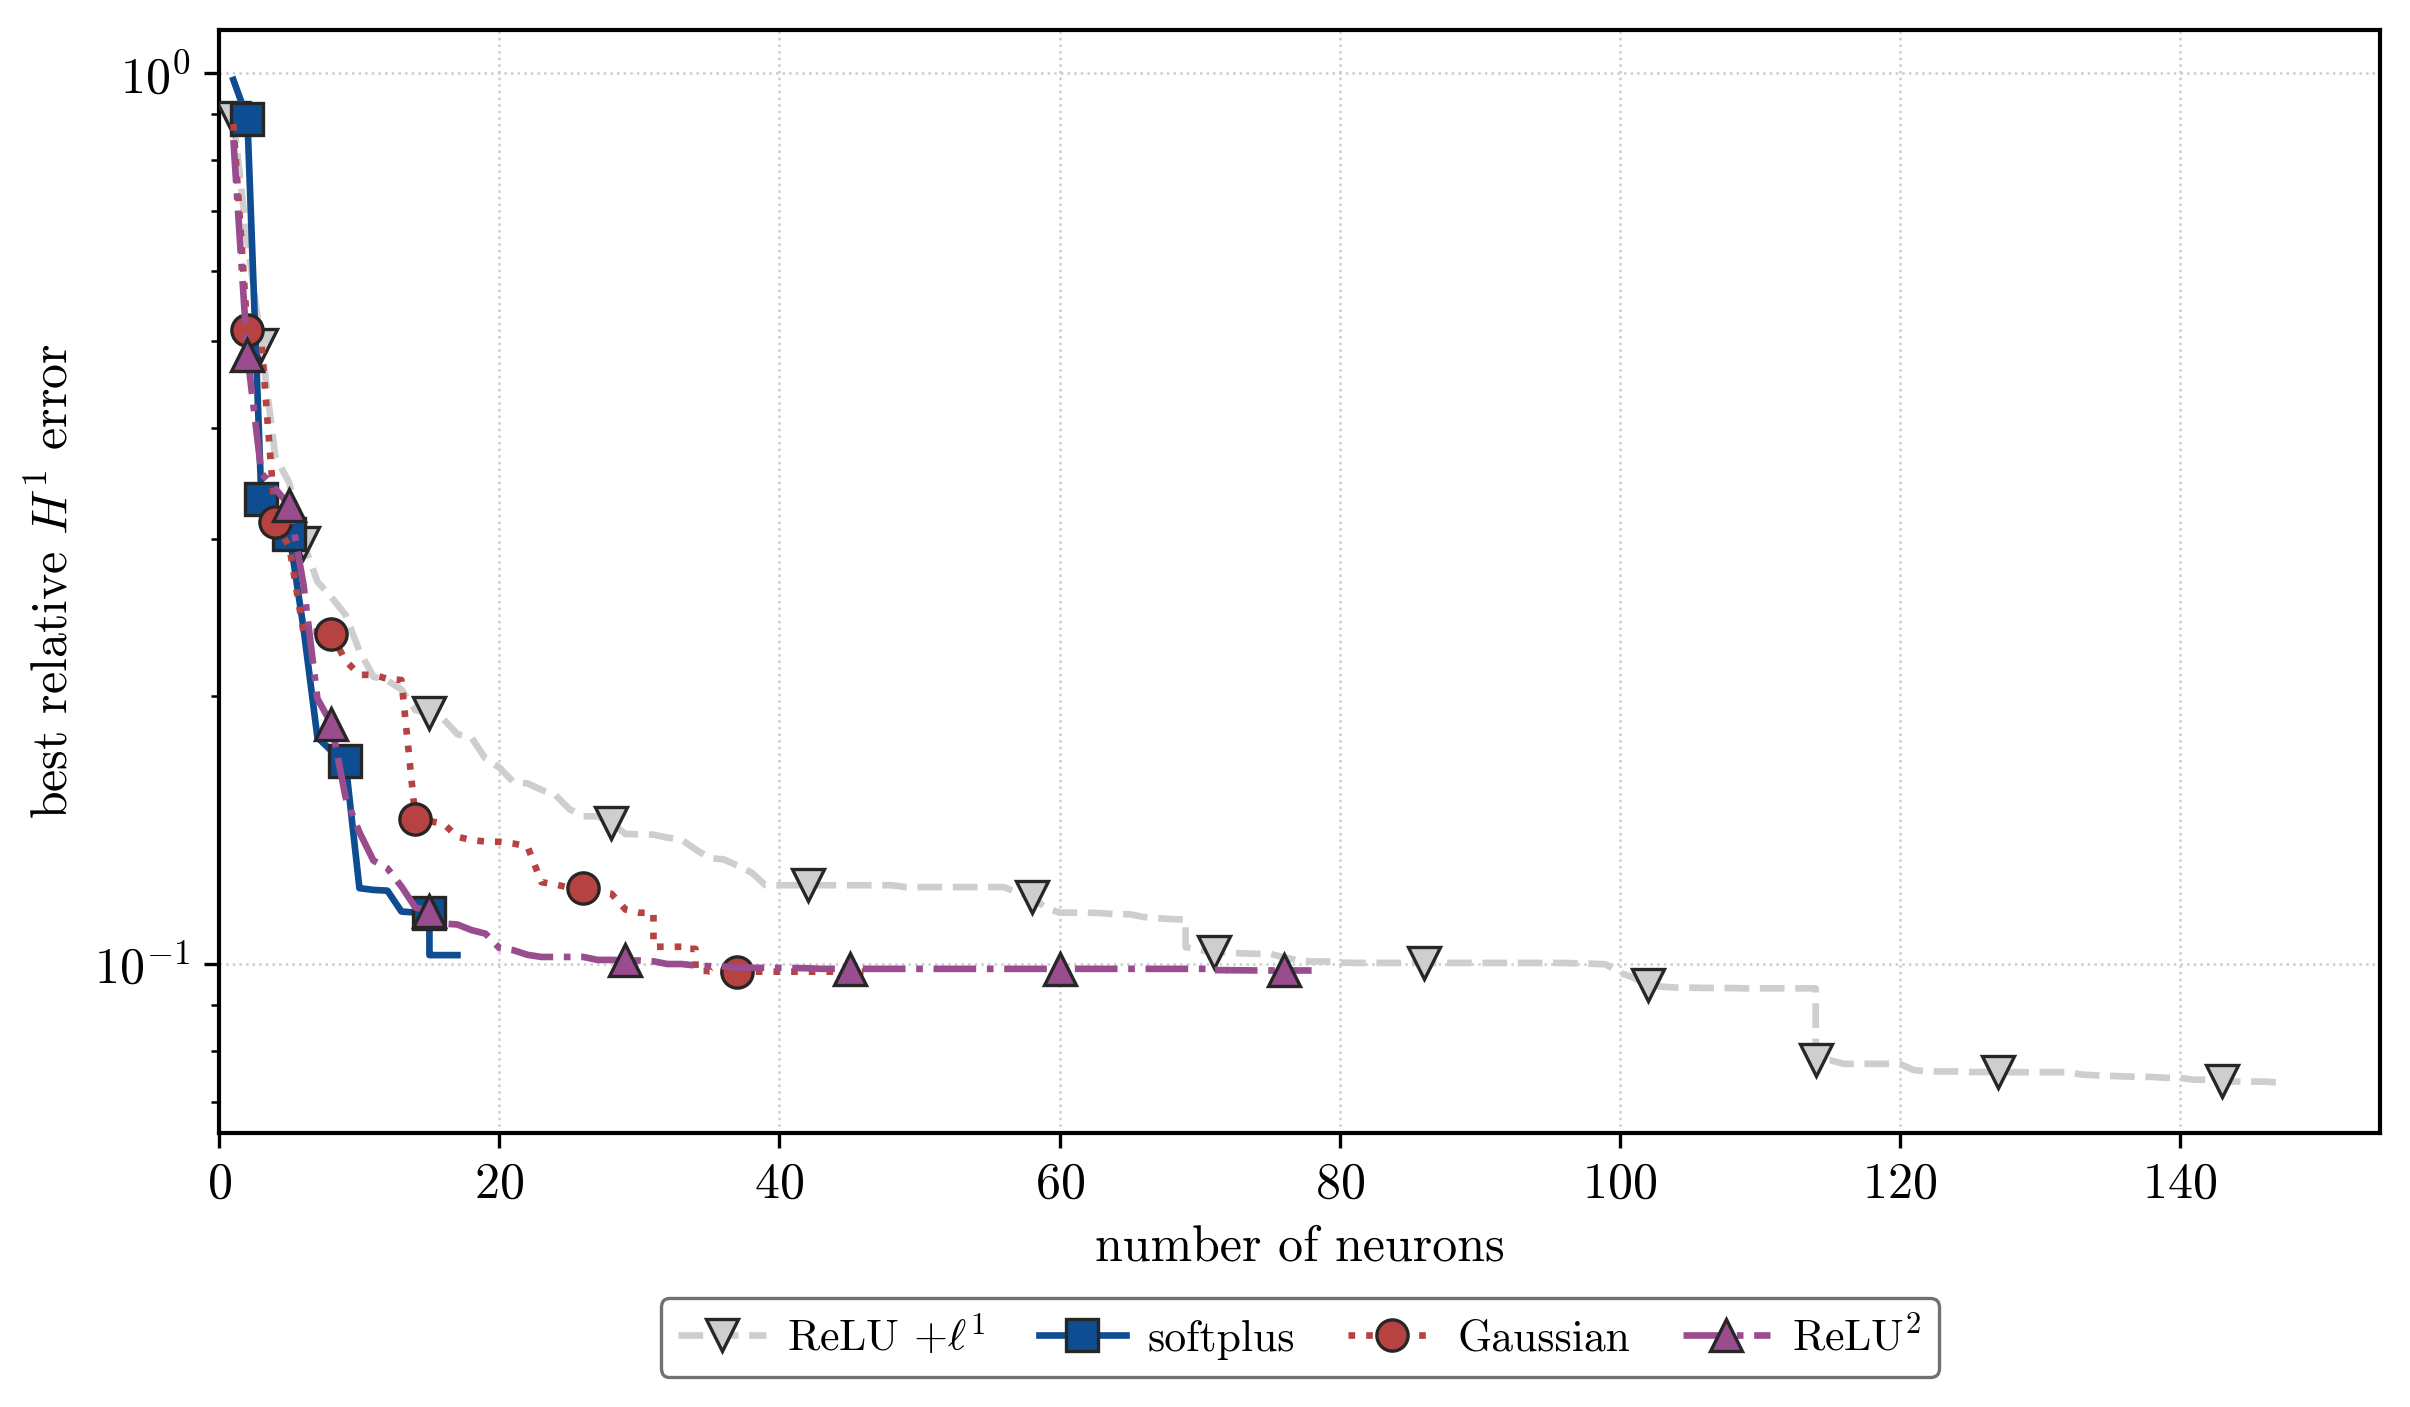
\includegraphics[width=\textwidth]{../experiments/01_vdp/paper_log_penalty/figures/frontier_intro.png}
\caption{Van der Pol accuracy against width.}
\label{fig:frontier_vdp}
\end{subfigure}
\hfill
\begin{subfigure}[b]{0.47\textwidth}
\centering
\small
\setlength{\tabcolsep}{4pt}
\renewcommand{\arraystretch}{1.18}
\begin{tabular}{lcc}
\toprule
Feedback law & cost & upright \\
\midrule
reference (PMP) & $26.2$ & yes \\
ReLU $+\ell^1$ & $265.4$ & no \\
\midrule
Gaussian & $8451.8$ & no \\
softplus & $69.8$ & yes \\
$\tanh$ & $7822.2$ & no \\
\midrule
$\mathrm{ReLU}^{2} + \psi_{2}$ & $60.4$ & yes \\
$\mathrm{ReLU}^{3} + \psi_{3}$ & $103.2$ & yes \\
\bottomrule
\end{tabular}
\caption{Pendulum feedback from start $A$.}
\label{fig:feedback_cost_a}
\end{subfigure}
\caption{Panel (a) shows the running
best relative $H^1$ validation error as neurons are inserted. Panel (b) gives
the closed-loop rollout cost from $A=(0.71,0.68)$ over $T=10$ and whether the
terminal state reaches the upright neighbourhood, defined by
$\operatorname{dist}(\theta,2\pi\mathbb Z)<0.4$ and $|\dot\theta|<0.4$.
The nonhomogeneous models use Algorithm~\ref{alg:log}
with $(\alpha,\gamma,p)=(10^{-4},10,2.01)$; the ReLU--$\ell^1$ baseline and
the homogeneous models use Algorithm~\ref{alg:q} at the most accurate
$\alpha$ for each $k$.}
\label{fig:neuron_h1_frontier}
\end{figure}


\section{Preliminaries}
This section reviews the measure-theoretic facts used in the paper. The
learning objectives and problem-specific assumptions are introduced in
Section~3.

\subsection{Finite signed Radon measures}
Let $\Omega$ be a locally compact Polish space. We write
$\mathcal M(\Omega)$ for the Banach space of finite signed Radon measures on
$\Omega$, equipped with the total-variation norm
\begin{equation*}
	\|\mu\|_{\mathcal M(\Omega)}:=|\mu|(\Omega).
\end{equation*}
By the Riesz representation theorem,
$\mathcal M(\Omega)=C_0(\Omega)^*$ under the pairing
\begin{equation*}
	\langle f,\mu\rangle:=\int_\Omega f\,d\mu.
\end{equation*}
Here $C_0(\Omega)$ denotes the continuous functions vanishing at infinity.

For $\mu \in \mathcal{M}(\Omega)$ we define the \emph{atom set}
$\atom \mu := \{\omega \in \Omega : |\mu|(\{\omega\}) > 0\}$, which is at most
countable, the purely atomic part
$\mu_{\atom} := \sum_{\omega \in \atom\mu} \mu(\{\omega\})\, \delta_\omega$,
and the nonatomic part $\mu_{\cont} := \mu - \mu_{\atom}$
\cite{bouchitte1990new}. This gives the decomposition
$\mu=\mu_{\cont}+\mu_{\atom}$.
The atom set need not be closed because atoms may accumulate at a point that
carries no mass.
The polar decomposition of a signed measure is written as
\begin{equation*}
	\mu=\sign(\mu)\,|\mu|,
	\qquad
	\sign(\mu):=\frac{d\mu}{d|\mu|}\in\{-1,1\}
	\quad |\mu|\text{-almost everywhere}.
\end{equation*}

\subsection{Measures with a finite moment}
In this subsection let $\Omega=\mathbb R^{d_\Omega}$, where
$d_\Omega\ge1$. For $p>0$, set
\begin{equation*}
	w_p(\omega):=1+|\omega|^p
\end{equation*}
and define
\begin{equation}
\label{eq:moment-space}
	\mathcal M_p(\Omega):=
	\left\{\mu\in\mathcal M(\Omega):
	\int_\Omega w_p\,d|\mu|<\infty\right\},
	\qquad
	\|\mu\|_{\mathcal M_p(\Omega)}:=
	\int_\Omega w_p\,d|\mu|.
\end{equation}
The associated space of continuous functions is
\begin{equation*}
	C_{w_p^{-1}}(\Omega):=
	\left\{f\in C(\Omega):\frac{f}{w_p}\in C_0(\Omega)\right\},
	\qquad
	\|f\|_{C_{w_p^{-1}}}:=
	\sup_{\omega\in\Omega}\frac{|f(\omega)|}{w_p(\omega)}.
\end{equation*}
Under the dual pairing,
$\mathcal M_p(\Omega)=C_{w_p^{-1}}(\Omega)^*$ isometrically
\cite[Section~5]{bartolucci-et-al}. For an atomic measure,
\begin{equation*}
	\left\|\sum_{j=1}^N c_j\delta_{\omega_j}\right\|_{\mathcal M_p(\Omega)}
	=\sum_{\eta\in\{\omega_1,\ldots,\omega_N\}}
	\left|\sum_{j:\,\omega_j=\eta}c_j\right|w_p(\eta).
\end{equation*}

\subsection*{Notation}
Throughout the remainder of the paper, $D\subset\mathbb R^d$ is a bounded
Lipschitz domain, $\nu:=\mathcal L^d|_D$ is the population measure,
and $L^2(D)$ means $L^2(D,\nu)$. We assume that the population target
$V$ belongs to $H^1(D)$. The symbol $M\ge1$ denotes the number of samples in
an empirical loss. The inner-parameter domain is
$\Omega=\mathbb R^{d+1}$, and $\rho\in C(\mathbb R)$ denotes the fixed
activation function of \eqref{eq:network}, with
\begin{equation*}
	\omega=(a,b),\qquad [K(\omega)](x):=\rho(a\cdot x+b).
\end{equation*}
With this notation, the network in \eqref{eq:network} is
$\mathcal N_{\boldsymbol\omega,c}=\sum_{n=1}^Nc_nK(\omega_n)$.
The symbol $\delta_\omega$ denotes the Dirac measure at $\omega$. 
We reserve $p$ for the moment order.

\section{The learning problem}

\subsection{The value operator and the gradient-augmented loss}
The finite network $\mathcal N_{\boldsymbol\omega,c}$ corresponds to the
finite atomic measure $\mu_{\boldsymbol\omega,c}$. This motivates the integral
formulation below, which agrees exactly with the finite sum on atomic
measures.

\begin{assumption}[Regularity and polynomial growth of $\rho$]
\label{ass:value-growth}
The activation satisfies $\rho\in C^1(\mathbb R)$. There are
$C_\rho>0$, $s_0\ge0$, and $s_1\ge\max\{s_0,1\}$ such that
\begin{enumerate}
	\item $|\rho(z)| \le C_\rho (1 + |z|)^{s_0}$ for every $z \in \mathbb{R}$;
	\item $|\rho'(z)| \le C_\rho (1 + |z|)^{s_1-1}$ for every
	$z \in \mathbb{R}$.
\end{enumerate}
\end{assumption}
Since $D$ is bounded, Assumption~\ref{ass:value-growth} gives constants
$C_D,C_K>0$ such that
\begin{equation}
	\label{eq:atom-L2-growth}
	\|K(\omega)\|_{L^2(D)} \le C_D (1 + |\omega|)^{s_0}.
\end{equation}
Moreover,
$\nabla K(a,b)(x)=a\rho'(a\cdot x+b)$, and hence
\begin{equation}
	\label{eq:H1-growth}
	\|K(\omega)\|_{H^1(D)}
	\le C_K(1+|\omega|)^{s_1}.
\end{equation}
If $\omega_n\to\omega$, their pre-activations lie in a common compact
interval on $D$. Uniform continuity of $\rho$ and $\rho'$ on that interval,
together with $a_n\to a$, therefore gives
$K(\omega_n)\to K(\omega)$ in $H^1(D)$. Thus
$K:\Omega\to H^1(D)$ is continuous and, in particular, strongly measurable.

For $\mu\in\mathcal M(\Omega)$ satisfying
\begin{equation}
\label{eq:H1-Bochner-condition}
	\int_\Omega\|K(\omega)\|_{H^1(D)}\,d|\mu|(\omega)<\infty,
\end{equation}
define the $H^1(D)$-valued Bochner integral
\begin{equation*}
	\mathcal N\mu:=\int_\Omega K(\omega)\,d\mu(\omega).
\end{equation*}
By \eqref{eq:H1-growth}, condition~\eqref{eq:H1-Bochner-condition} holds for
$\mu\in\mathcal M_p(\Omega)$ when $p>s_1$. For
$\psi\in C_c^\infty(D)$ and $i\in\{1,\ldots,d\}$, the growth bound permits
Fubini's theorem and gives
\begin{align*}
	\int_D(\mathcal N\mu)\,\partial_i\psi\,dx
	&=\int_\Omega\int_D K(\omega)\,\partial_i\psi\,dx\,d\mu(\omega)\\
	&=-\int_D\left(\int_\Omega\partial_iK(\omega)\,d\mu(\omega)\right)
	\psi\,dx.
\end{align*}
Consequently,
\begin{equation*}
	\nabla(\mathcal N\mu)
	=\int_\Omega\nabla K(\omega)\,d\mu(\omega)
	\quad\text{in }L^2(D;\mathbb R^d).
\end{equation*}
For measures satisfying only
$\int_\Omega\|K(\omega)\|_{L^2(D)}\,d|\mu|(\omega)<\infty$, the same
definition is valid as an $L^2(D)$-valued Bochner integral. By
\eqref{eq:atom-L2-growth}, this includes $\mathcal M_p(\Omega)$ when
$p>s_0$. In particular,
$\mathcal N\mu_{\boldsymbol\omega,c}=\mathcal N_{\boldsymbol\omega,c}$.
Whenever $\mathcal N\mu\in H^1(D)$, set
$r_\mu:=\mathcal N\mu-V$.

The fidelity term is the gradient-augmented loss with the distributional
gradient convention. If the $L^2(D)$-valued integral defining
$\mathcal N\mu$ does not exist, we set $L(\mu)=+\infty$; otherwise,
\begin{equation*}
	L(\mu) :=
	\begin{cases}
	\dfrac{1}{2} \|\mathcal{N}\mu - V \|^2_{L^2(D)}
	+ \dfrac{1}{2} \|\nabla(\mathcal{N}\mu) - \nabla V \|_{L^2(D)}^2,
	& \mathcal{N}\mu \in H^1(D),\\[4pt]
	+\infty, & \text{otherwise.}
	\end{cases}
\end{equation*}

For sampled labels $(V(x^m),g^m)_{m=1}^M$ and a finite network for which the
displayed point values exist, the corresponding empirical fidelity is
\begin{equation}
\label{eq:empirical-fidelity}
	l^M(\mu):=
	\frac{1}{2M}\sum_{m=1}^M
	\left(
	|\mathcal N\mu(x^m)-V(x^m)|^2
	+|\nabla\mathcal N\mu(x^m)-g^m|^2
	\right).
\end{equation}

\subsection{The nonconvex functional}
Let $\phi:\mathbb{R}_+\to\mathbb{R}_+$ satisfy the following assumptions.
\begin{assumption}\label{pen1}
The finite right derivative
\begin{equation*}
	L_\phi:=\phi'(0+)
\end{equation*}
exists and satisfies $0<L_\phi<\infty$. We use the convention $\phi'(0):=L_\phi$.
\end{assumption}

\begin{assumption}\label{pen2}
The function $\phi$ is concave, nondecreasing, and coercive, with
$\phi(0)=0$, and belongs to $C^1((0,\infty))$.
\end{assumption}

Assumptions~\ref{pen1} and~\ref{pen2} imply that $\phi'(t)>0$ for every
$t>0$. Indeed, if
$\phi'(t_0)=0$ at some $t_0>0$, concavity and monotonicity would give
$\phi'(t)=0$ for every $t\ge t_0$, making $\phi$ constant there and
contradicting coercivity. Hence $\phi$ is continuous and strictly increasing
from $[0,\infty)$ onto $[0,\infty)$. We denote its inverse by $\phi^{-1}$.

\begin{assumption}[Local curvature]\label{pen3}
The function $\phi$ belongs to $C^2((0,\infty))$ and satisfies both of the
following conditions:
\begin{enumerate}
	\item there are $\gamma_1\ge0$ and $\hat z_1>0$ such that
	$-\gamma_1(z_2-z_1)\le\phi'(z_2)-\phi'(z_1)\le0$
	for $0\le z_1\le z_2\le\hat z_1$;
	\item for every $A>0$,
	\begin{equation*}
		\gamma_A:=-\sup_{0<t\le A}\phi''(t)>0.
	\end{equation*}
\end{enumerate}
\end{assumption}

\begin{remark}
The lower curvature control in Assumption~\ref{pen3}(1) is local and does not
follow from global concavity. For example,
$\phi(z)=z-\frac23z^{3/2}$ near the origin has
$\phi''(z)=-\frac12z^{-1/2}$; it can be extended linearly after a small
positive point so as to remain nondecreasing, concave, and coercive.
\end{remark}

\begin{lemma}\label{firstorderestimate}
Let $\phi:[0,\infty)\to[0,\infty)$ be concave with
$\phi(0)=0$. Then
\begin{enumerate}
	\item $\phi(z_1+z_2)\le\phi(z_1)+\phi(z_2)$ for all $z_1,z_2\ge0$.
\end{enumerate}
If in addition $L_\phi:=\phi'(0+)$ is finite, then
\begin{enumerate}
	\setcounter{enumi}{1}
	\item $\phi(z)\le L_\phi z$ for all $z\ge0$;
	\item $\phi(z)/z\longrightarrow L_\phi$ as $z\downarrow0$;
	\item for every nonnegative sequence $(t_j)_{j\ge1}$ with
	$\sum_{j\ge1}t_j<\infty$,
	\begin{equation*}
		\phi\left(\sum_{j\ge1}t_j\right)
		\le\sum_{j\ge1}\phi(t_j).
	\end{equation*}
\end{enumerate}
\end{lemma}
\begin{proof}
Concavity and $\phi(0)=0$ make $z\mapsto\phi(z)/z$ nonincreasing on
$(0,\infty)$: for $0<z_1\le z_2$, writing
$z_1=\frac{z_1}{z_2}z_2+\bigl(1-\frac{z_1}{z_2}\bigr)\cdot0$ and using
concavity together with $\phi(0)=0$ gives
$\phi(z_1)\ge\frac{z_1}{z_2}\phi(z_2)$.

(1) Suppose without loss of generality that $0<z_1\le z_2$. Then
\begin{align*}
	\phi(z_1+z_2)
	&\le\frac{z_1+z_2}{z_2}\phi(z_2)
	&&\text{because $\phi(z)/z$ is nonincreasing}\\
	&=\phi(z_2)+z_1\frac{\phi(z_2)}{z_2}\\
	&\le\phi(z_2)+\phi(z_1)
	&&\text{by the same monotonicity}.
\end{align*}
The cases with $z_1=0$ or $z_2=0$ follow from $\phi(0)=0$.

(2) and (3) By the same monotonicity and $\phi(0)=0$,
\begin{equation*}
	\frac{\phi(z)}z
	\le\lim_{s\downarrow0}\frac{\phi(s)}s
	=\lim_{s\downarrow0}\frac{\phi(s)-\phi(0)}{s}
	=L_\phi
	\qquad(z>0),
\end{equation*}
and the displayed limit is precisely~(3).

(4) By~(2) the function $\phi$ is continuous at $0$, and a finite concave
function is continuous on $(0,\infty)$. Iterating~(1) over partial sums gives
\begin{equation*}
	\phi\Bigl(\sum_{j\le N}t_j\Bigr)
	\le\sum_{j\le N}\phi(t_j)
	\le\sum_{j\ge1}\phi(t_j),
\end{equation*}
the last step because the terms are nonnegative. Letting $N\to\infty$ and
using continuity of $\phi$ at $\sum_{j\ge1}t_j$ proves the claim.
\end{proof}

Assumption~\ref{pen2} implies the standing hypotheses of
Lemma~\ref{firstorderestimate}, and Assumption~\ref{pen1} supplies the finite
right slope needed for parts~(2)--(4). Neither coercivity nor differentiability
on $(0,\infty)$ is used, so the lemma also applies under the weaker hypotheses
of Theorem~\ref{thm:phi-lsc}.


\begin{proposition}[Second-order bounds]\label{secondorderestimate}
Suppose that $\phi(0)=0$ and Assumption~\ref{pen1} holds.
\begin{enumerate}
	\item If the derivative bound in Assumption~\ref{pen3}(1) holds, then
	$\phi(z)\ge L_\phi z-\frac{\gamma_1}{2}z^2$ for
	$0\le z\le\hat z_1$;
	\item if $\phi\in C^2((0,\infty))$ and Assumption~\ref{pen3}(2) holds,
	then, for every $A>0$,
	$\phi(z)\le L_\phi z-\frac{\gamma_A}{2}z^2$ for
	$0\le z\le A$.
\end{enumerate}
\end{proposition}
\begin{proof}
For $\varepsilon>0$, apply the fundamental theorem of calculus on
$[\varepsilon,z]$ and then let $\varepsilon\downarrow0$. The definition of
the finite right derivative and $\phi(0)=0$ give
\begin{equation*}
	\phi(z)-L_\phi z
	=\int_0^z[\phi'(s)-L_\phi]\,ds.
\end{equation*}
The first conclusion follows from Assumption~\ref{pen3}(1). For the second,
Assumption~\ref{pen3}(2) gives
$\phi''(t)\le-\gamma_A$ on $(0,A]$. Integrating from $\varepsilon$ to $s$
and then letting $\varepsilon\downarrow0$ gives
$\phi'(s)-L_\phi\le-\gamma_A s$ for $0<s\le A$. Integration proves the
claim.
\end{proof}

For an open set $U\subset\Omega$, let $C_c(U)$ denote the continuous
functions with compact support in $U$.
Define
\begin{equation}
\label{eq:concave-measure-functional}
	\Phi_\phi(\mu)
	:=L_\phi\|\mu_{\cont}\|_{\mathcal M(\Omega)}
	+\sum_{\omega\in\atom\mu}
		\phi\bigl(|\mu(\{\omega\})|\bigr),
	\qquad \mu\in\mathcal M(\Omega).
\end{equation}

\begin{lemma}
\label{lem:phi-coercivity}
Let $U\subset\Omega=\mathbb R^{d+1}$ be open, let
$\mu\in\mathcal M(U)$, and let $\delta>0$. Suppose that
\begin{equation*}
	|\mu(\{\omega\})|\le\frac{\delta}{4}
	\qquad\text{for every }\omega\in U.
\end{equation*}
Then, for every $\varepsilon>0$, there are $m\ge1$ and functions
$h_1,\ldots,h_m\in C_c(U)$ with pairwise disjoint supports and
$|h_i|\le1$ such that
\begin{equation*}
	\left|\int_U h_i\,d\mu\right|\le\delta
	\quad (i=1,\ldots,m),
	\qquad
	\sum_{i=1}^m\left|\int_U h_i\,d\mu\right|
	\ge\|\mu\|_{\mathcal M(U)}-\varepsilon.
\end{equation*}
\end{lemma}
\begin{proof}
If $\varepsilon\ge\|\mu\|_{\mathcal M(U)}$, take $m=1$ and $h_1=0$.
Henceforth assume $0<\varepsilon<\|\mu\|_{\mathcal M(U)}$.
Let $U=P\cup N$ be a Hahn decomposition of $\mu$. By inner
regularity, there are disjoint compact sets $K_+\subset P$ and $K_-\subset N$
such that
\begin{equation}
\label{eq:phi-hahn-compact-loss}
	|\mu|\bigl(U\setminus(K_+\cup K_-)\bigr)<\frac{\varepsilon}{4}.
\end{equation}

We now construct the required finite small-mass partition, including both the
atomic and nonatomic parts. For every $\omega\in K_+\cup K_-$, continuity from
above gives
\begin{equation*}
	|\mu|\bigl(B_r(\omega)\bigr)
	\longrightarrow |\mu|(\{\omega\})
	\le\frac{\delta}{4}
	\qquad(r\downarrow0).
\end{equation*}
Choose $r_\omega>0$ such that
$|\mu|(B_{r_\omega}(\omega))<\delta/2$. Compactness gives a finite subcover
Let $B_1,\ldots,B_N$ be these balls. For each
$\sigma\in\{+,-\}$, define inductively
\begin{equation*}
E_i^\sigma
:=(K_\sigma\cap B_i)
\setminus\bigcup_{j<i}(K_\sigma\cap B_j),
\qquad i=1,\ldots,N,
\end{equation*}
where the union is empty for $i=1$. After discarding empty sets, the
$E_i^\sigma$ form a pairwise disjoint Borel partition of $K_\sigma$, with
$E_i^\sigma\subset B_i$.
A finite Borel partition $E_1,\ldots,E_{m_0}$ for some $m_0\ge1$ of
$K_+\cup K_-$ is constructed such that each
$E_i$ lies in either $P$ or $N$ and 
$|\mu|(E_i)<\delta/2$.

By inner regularity, choose compact sets $C_i\subset E_i$ whose total omitted
mass is less than $\varepsilon/4$, and discard the empty sets. At least one
set remains because $\varepsilon<\|\mu\|_{\mathcal M(U)}$ and
\eqref{eq:phi-hahn-compact-loss}. Relabel the remaining sets
$C_1,\ldots,C_m$. They are pairwise disjoint and satisfy
\begin{equation}
\label{eq:phi-core-loss}
	\sum_{i=1}^m|\mu|(C_i)
	\ge |\mu|(K_+\cup K_-)-\frac{\varepsilon}{4},
	\qquad
	|\mu|(C_i)\le\frac{\delta}{2}.
\end{equation}
Each $C_i$ lies entirely in either $P$ or $N$.

Because the compact sets $C_i$ are finitely many, pairwise disjoint, and
contained in the open set $U$, they have pairwise disjoint relatively compact
open neighborhoods. Outer regularity lets us shrink these neighborhoods,
while keeping each $C_i$ inside, to obtain open sets $U_i$ satisfying
\begin{equation}
\label{eq:phi-neighborhood-loss}
	\sum_{i=1}^m|\mu|(U_i\setminus C_i)
	<\min\left\{\frac{\varepsilon}{4},\frac{\delta}{2}\right\}.
\end{equation}
For each $i$, the continuous function
\begin{equation*}
	\chi_i(\omega)
	:=\frac{\operatorname{dist}(\omega,U_i^c)}
	{\operatorname{dist}(\omega,C_i)+\operatorname{dist}(\omega,U_i^c)}
\end{equation*}
equals one on $C_i$, vanishes outside $U_i$, and has compact support in $U$.
Set $h_i=\chi_i$ when $C_i\subset P$ and $h_i=-\chi_i$ when $C_i\subset N$.
Their supports are pairwise disjoint and $|h_i|\le1$. Moreover,
\begin{align*}
	\left|\int_U h_i\,d\mu\right|
	&\le |\mu|(U_i)
	\le |\mu|(C_i)+|\mu|(U_i\setminus C_i)
	\le\delta,
	&&\text{by \eqref{eq:phi-core-loss}--\eqref{eq:phi-neighborhood-loss},}
\end{align*}
and
\begin{align*}
	\sum_{i=1}^m\left|\int_U h_i\,d\mu\right|
	&\ge \sum_{i=1}^m
		\bigl(|\mu|(C_i)-|\mu|(U_i\setminus C_i)\bigr)\\
	&\ge |\mu|(K_+\cup K_-)
		-\frac{\varepsilon}{4}-\frac{\varepsilon}{4}
	&&\text{by \eqref{eq:phi-core-loss}--\eqref{eq:phi-neighborhood-loss},}\\
	&\ge \|\mu\|_{\mathcal M(U)}
		-\frac{\varepsilon}{4}-\frac{\varepsilon}{4}-\frac{\varepsilon}{4}
	&&\text{by \eqref{eq:phi-hahn-compact-loss},}\\
	&=\|\mu\|_{\mathcal M(U)}-\frac{3\varepsilon}{4}.
\end{align*}
This is stronger than the required lower bound.
\end{proof}

\begin{theorem}[Representation formula for the nonconvex functional]
\label{thm:phi-lsc}
Suppose that $\phi:[0,\infty)\to[0,\infty)$ is nondecreasing and concave,
$\phi(0)=0$, and
\begin{equation*}
	L_\phi:=\phi'(0+)\in(0,\infty).
\end{equation*}
Then, for every $\mu\in\mathcal M(\Omega)$,
\begin{equation}
\label{eq:phi-disjoint-representation}
	\Phi_\phi(\mu)
	=\sup\left\{
	\sum_{i=1}^m\phi\left(\left|\int_\Omega f_i\,d\mu\right|\right):
	\begin{array}{l}
		m\ge1,\quad f_i\in C_c(\Omega),\quad |f_i|\le1,\\
		\supp(f_i)\text{ are pairwise disjoint}
	\end{array}
	\right\}.
\end{equation}
\end{theorem}
\begin{proof}
We prove the representation by first bounding every admissible finite sum
from above and then constructing sums that approach
$\Phi_\phi(\mu)$ from below. The hypotheses are exactly the standing
hypotheses of Lemma~\ref{firstorderestimate} together with
$L_\phi\in(0,\infty)$, so parts~(1)--(3) of that lemma give
\begin{equation}
\label{eq:phi-basic-bounds}
	\phi(r+s)\le\phi(r)+\phi(s),
	\qquad
	\phi(r)\le L_\phi r,
	\qquad
	\frac{\phi(r)}{r}\longrightarrow L_\phi
	\quad(r\downarrow0),
\end{equation}
and part~(4) gives the countable form
$\phi\bigl(\sum_{j\ge1}t_j\bigr)\le\sum_{j\ge1}\phi(t_j)$.

Write the atomic part of $\mu$ as
\begin{equation*}
	\mu_{\atom}=\sum_{j\ge1}c_j\delta_{\omega_j},
\end{equation*}
where the $\omega_j$ are distinct and $c_j\ne0$. For an admissible family
$(f_i)_{i=1}^m$, set
\begin{equation*}
	A_i:=\sum_{j\ge1}|c_j|\,|f_i(\omega_j)|,
	\qquad
	B_i:=\int_\Omega|f_i|\,d|\mu_{\cont}|.
\end{equation*}

\begin{align*}
	\phi\left(\left|\int_\Omega f_i\,d\mu\right|\right)
	&\le \phi(A_i+B_i)
	&&\text{by the triangle inequality}\\
	&\le \sum_{\omega_j\in\supp(f_i)}\phi(|c_j|)+L_\phi B_i
	&&\text{by Lemma~\ref{firstorderestimate}(2),~(4) and }|f_i|\le1.
\end{align*}
The disjoint supports count each atom at most once and satisfy
$\sum_i|f_i|\le1$. Therefore
\begin{align*}
	\sum_{i=1}^m
	\phi\left(\left|\int_\Omega f_i\,d\mu\right|\right)
	&\le \sum_{j\ge1}\phi(|c_j|)
	+L_\phi\int_\Omega\sum_{i=1}^m|f_i|\,d|\mu_{\cont}|\\
	&\le \sum_{j\ge1}\phi(|c_j|)
	+L_\phi\|\mu_{\cont}\|_{\mathcal M(\Omega)}
	=\Phi_\phi(\mu).
\end{align*}
This proves the upper bound in \eqref{eq:phi-disjoint-representation}.

For the reverse inequality, the claim is immediate when $\mu=0$. Otherwise,
fix $\varepsilon>0$. Choose
$\theta\in(0,L_\phi)$ such that
$\theta\|\mu\|_{\mathcal M(\Omega)}<\varepsilon/4$. By the last limit in
\eqref{eq:phi-basic-bounds}, choose $\delta>0$ such that
\begin{equation}
\label{eq:phi-linear-near-zero}
	\phi(r)\ge(L_\phi-\theta)r
	\qquad(0\le r\le\delta).
\end{equation}
Let
\begin{equation*}
	F:=\{j\ge1:|c_j|>\delta/8\},
	\qquad
	\mu_{\mathrm{rem}}
	:=\mu-\sum_{j\in F}c_j\delta_{\omega_j}.
\end{equation*}
The set $F$ is finite and every point mass of $\mu_{\mathrm{rem}}$ has
magnitude at most $\delta/8$.

Because $F$ is finite, its points have pairwise disjoint relatively compact
neighborhoods. Moreover,
$\mu_{\mathrm{rem}}(\{\omega_j\})=0$ for $j\in F$, so continuity of the measure from above
allows these neighborhoods to be chosen with arbitrarily small total
$|\mu_{\mathrm{rem}}|$-mass. Using the distance-function construction from
Lemma~\ref{lem:phi-coercivity}, choose $g_j\in C_c(\Omega)$, $j\in F$, with
pairwise disjoint supports, $|g_j|\le1$, and
\begin{equation*}
	g_j(\omega_j)=\sign(c_j),
	\qquad
	\sum_{j\in F}|\mu_{\mathrm{rem}}|(\supp(g_j))<\tau,
\end{equation*}
where $\tau>0$ can be chosen arbitrarily small. For every $j\in F$,
\begin{equation*}
	\left|
	\left|\int_\Omega g_j\,d\mu\right|-|c_j|
	\right|
	\le |\mu_{\mathrm{rem}}|(\supp(g_j)).
\end{equation*}
By continuity of $\phi$ and finiteness of $F$, first choose $\tau$
sufficiently small and then choose the supports so that
\begin{equation}
\label{eq:phi-large-atom-tests}
	\sum_{j\in F}
	\phi\left(\left|\int_\Omega g_j\,d\mu\right|\right)
	\ge\sum_{j\in F}\phi(|c_j|)-\frac{\varepsilon}{4},
	\qquad
	2L_\phi\tau<\frac{\varepsilon}{4}.
\end{equation}

Set
\begin{equation*}
	U:=\Omega\setminus\bigcup_{j\in F}\supp(g_j)
	\qquad\text{and}\qquad
	\lambda:=\mu_{\mathrm{rem}}|_U.
\end{equation*}
Lemma~\ref{lem:phi-coercivity} applied on the open set $U$ gives
$h_1,\ldots,h_m\in C_c(U)$ whose zero extensions belong to $C_c(\Omega)$,
have pairwise disjoint supports, and satisfy
\begin{equation*}
	\left|\int_Uh_i\,d\lambda\right|\le\delta,
	\qquad
	\sum_{i=1}^m\left|\int_Uh_i\,d\lambda\right|
	\ge\|\lambda\|_{\mathcal M(U)}-\tau
	\ge\|\mu_{\mathrm{rem}}\|_{\mathcal M(\Omega)}-2\tau.
\end{equation*}
Together with the $g_j$, the zero extensions form an admissible family in
\eqref{eq:phi-disjoint-representation}. Since every $h_i$ is supported in
$U$ and $\mu|_U=\lambda$, its integrals against $\mu$ and $\lambda$ agree.
Therefore \eqref{eq:phi-linear-near-zero} and
\eqref{eq:phi-large-atom-tests} yield
\begin{align*}
	&\sum_{j\in F}
	\phi\left(\left|\int_\Omega g_j\,d\mu\right|\right)
	+\sum_{i=1}^m
	\phi\left(\left|\int_\Omega h_i\,d\mu\right|\right)\\
	&\quad\ge
	\sum_{j\in F}\phi(|c_j|)-\frac{\varepsilon}{4}
	+(L_\phi-\theta)
	\bigl(\|\mu_{\mathrm{rem}}\|_{\mathcal M(\Omega)}-2\tau\bigr)\\
	&\quad\ge
	\Phi_\phi(\mu)-\frac{\varepsilon}{4}
	-\theta\|\mu_{\mathrm{rem}}\|_{\mathcal M(\Omega)}-2L_\phi\tau
	&&\text{by }\Phi_\phi(\mu_{\mathrm{rem}})
	\le L_\phi\|\mu_{\mathrm{rem}}\|_{\mathcal M(\Omega)}\\
	&\quad>\Phi_\phi(\mu)-\varepsilon.
\end{align*}
Taking the supremum and then letting $\varepsilon\downarrow0$ proves the
reverse inequality.
\end{proof}

\begin{corollary}
\label{cor:phi-lsc-sublevels}
Under the assumptions of Theorem~\ref{thm:phi-lsc}, the functional
$\Phi_\phi$ is weak-* lower semicontinuous on
$\mathcal M(\Omega)=C_0(\Omega)^*$. If $\phi$ is also coercive, then every
sublevel of $\Phi_\phi$ is bounded in total variation.
\end{corollary}
\begin{proof}
For each fixed admissible family in
\eqref{eq:phi-disjoint-representation}, weak-* convergence gives convergence
of all its integrals, and continuity of $\phi$ gives convergence of the
corresponding finite sum. The representation is a supremum of weak-*
continuous functions and is therefore weak-* lower semicontinuous.

For the sublevel bound, apply repeated subadditivity to the first $N$ atoms
and let $N\to\infty$. The atom magnitudes are summable, so continuity of
$\phi$ gives
\begin{equation*}
	\phi\bigl(\|\mu_{\atom}\|_{\mathcal M(\Omega)}\bigr)
	\le\sum_{\omega\in\atom\mu}
		\phi\bigl(|\mu(\{\omega\})|\bigr)
	\le\Phi_\phi(\mu),
	\qquad
	L_\phi\|\mu_{\cont}\|_{\mathcal M(\Omega)}
	\le\Phi_\phi(\mu).
\end{equation*}
If $\Phi_\phi(\mu)\le C$, coercivity bounds
$\|\mu_{\atom}\|_{\mathcal M(\Omega)}$ in terms of $C$, while
$\|\mu_{\cont}\|_{\mathcal M(\Omega)}\le C/L_\phi$. The atomic part is
supported on the countable atom set, while the continuous part assigns that
set zero variation. The two parts are therefore mutually singular, so their
total-variation norms add to $\|\mu\|_{\mathcal M(\Omega)}$. Hence the
sublevel is bounded in total variation.
\end{proof}



\subsection{The normalized problem}
For $\alpha>0$, define
\begin{equation*}
	J_0(\mu):=L(\mu)+\alpha\Phi_\phi(\mu)
\end{equation*}
for the unnormalized problem on the parameter domain.


\subsubsection*{Escape on the unbounded parameter domain}
\label{sec:escape}
For positively homogeneous profiles the radial scale of $\omega$ is absorbed by
the outer coefficient, and the parameter can be restricted to the unit sphere
$\mathbb{S}^d$ (Section~4). But in general the domain is
$\Omega = \mathbb{R}^{d+1}$, which is not compact.
The regularizer $\Phi_\phi$ depends on the sizes of the
coefficients but not on the locations of the atoms. Along a sequence with
$|\omega|\to\infty$, the fidelity need not be lower
semicontinuous.

\begin{example}[Failure of weak-* lower semicontinuity for $\tanh$]
\label{ex:tanh_escape}
Let $\rho = \tanh$, $V \equiv 1$, fix $a\in\mathbb R^d$, and set
$\mu_n = \delta_{(a, b_n)}$ with $b_n \to \infty$. Then
$\mu_n \overset{*}{\rightharpoonup} 0$, yet
\begin{equation*}
	\mathcal{N}\mu_n = \tanh(a \cdot x + b_n) \to 1
\end{equation*}
strongly in $H^1(D)$. Hence
$\liminf_{n\to\infty} L(\mu_n) = 0 < L(0)$, so the fidelity term is not
weak-* lower semicontinuous. Mass escaping to infinity carries a non-vanishing
value contribution unless $K(\omega)$ tends to zero as $|\omega|\to\infty$.

Note that $\Phi_\phi(\mu_n) = \phi(1)$ is constant along this sequence, so the
unnormalized coefficient penalty does not prevent this escape. The defect is
that the unnormalized kernel does not vanish at parameter infinity. The
normalized atom introduced in Theorem~\ref{thm:normalization} does vanish
under the corresponding polynomial growth gap.
\end{example}

\begin{example}[Nonattainment for softplus]
\label{ex:softplus_escape}
For the profile $\rho(z) = \log(1 + e^z)$ (softplus), let $b_n\to\infty$.
The measures
$\mu_n = \rho(b_n)^{-1}\delta_{(0, b_n)}$ fit $V \equiv 1$ exactly for every
$n$ at penalty $\alpha\,\phi(1/\rho(b_n)) \to 0$, so $\inf J_0 = 0$ is not
attained. Indeed, if $J_0(\mu)=0$, then $\Phi_\phi(\mu)=0$. Strict positivity
of $\phi$ on $(0,\infty)$ and $L_\phi>0$ force both the atomic and continuous
parts of $\mu$ to vanish. Thus $\mu=0$, but
$L(0)=\frac12\|1\|_{H^1(D)}^2>0$, a contradiction.
\end{example}

We need a penalty that is aware of the location of the atom to prevent the escape. 
The space of measure of finite moment is the right space to work with. 
For $p>0$, let $w_p$ and $\mathcal M_p(\Omega)$ be as in
\eqref{eq:moment-space}. For $\mu\in\mathcal M_p(\Omega)$, we define the
normalized measure and normalized atom by
\begin{equation*}
	d\mu_p:=w_p\,d\mu,
	\qquad
	K_p(\omega):=\frac{K(\omega)}{w_p(\omega)}.
\end{equation*}

\begin{theorem}
\label{thm:normalization}
Multiplication by $w_p$ is a linear isometric bijection
\begin{equation*}
	\mathcal M_p(\Omega)\longrightarrow\mathcal M(\Omega),
	\qquad \mu\longmapsto\mu_p,
\end{equation*}
with inverse $d\mu=w_p^{-1}d\mu_p$, and
\begin{equation}
\label{eq:normalization-norm}
	\|\mu\|_{\mathcal M_p(\Omega)}
	=\|\mu_p\|_{\mathcal M(\Omega)}.
\end{equation}
Moreover, $\mu_n$ converges weak-* to $\mu$ in
$C_{w_p^{-1}}(\Omega)^*$ if and only if
$(\mu_n)_p\overset{*}{\rightharpoonup}\mu_p$ in $C_0(\Omega)^*$.
The multiplication preserves the atom set and the polar sign, and
\begin{equation}
\label{eq:normalization-decomposition}
	(\mu_p)_{\atom}=w_p\mu_{\atom},
	\qquad
	(\mu_p)_{\cont}=w_p\mu_{\cont}.
\end{equation}
If part~(1) of Assumption~\ref{ass:value-growth} holds and $p>s_0$, then
$K_p\in C_0(\Omega;L^2(D))$ and
\begin{equation}
\label{eq:normalization-output}
	\mathcal N\mu
	=\int_\Omega K\,d\mu
	=\int_\Omega K_p\,d\mu_p.
\end{equation}
Finally,
\begin{equation}
\label{eq:normalization-penalty}
	\Phi_\phi(\mu_p)
	=L_\phi\int_\Omega w_p\,d|\mu_{\cont}|
	+\sum_{\omega\in\atom\mu}
	\phi\bigl(w_p(\omega)|\mu(\{\omega\})|\bigr).
\end{equation}
\end{theorem}
\begin{proof}
The isometric identification with $\mathcal M(\Omega)$, including its inverse,
the norm identity, and the weak-* equivalence, is the polynomial-weight
specialization of \cite[Section~5.1]{bartolucci-et-al}; in particular, this
gives \eqref{eq:normalization-norm}. Since multiplication by the strictly
positive function $w_p$ preserves null sets, the atom set, the polar sign, and
nonatomicity, \eqref{eq:normalization-decomposition} follows immediately.

It remains to treat the network map. The continuity of $K_p$ follows from
that of $K$ and $w_p$. For $r=|\omega|\ge1$, the growth estimate
\eqref{eq:atom-L2-growth} gives
\begin{align*}
	\|K_p(\omega)\|_{L^2(D)}
	&\le C_D\frac{(1+r)^{s_0}}{1+r^p}\\
	&\le 2^{s_0}C_D r^{s_0-p}\longrightarrow0,
	\qquad r\to\infty,
\end{align*}
because $p>s_0$. Thus $K_p\in C_0(\Omega;L^2(D))$. The change-of-measure
identity for the Bochner integral now gives
\eqref{eq:normalization-output}. Finally,
\eqref{eq:normalization-decomposition} and
$|w_p\mu_{\cont}|=w_p|\mu_{\cont}|$ give
\eqref{eq:normalization-penalty} directly from
\eqref{eq:concave-measure-functional}.
\end{proof}

For $\alpha>0$, define the adopted objective
\begin{equation*}
	J(\mu):=
	L(\mu)+\alpha\Phi_\phi(\mu_p),
	\qquad \mu\in\mathcal M_p(\Omega).
\end{equation*}
For a finite atomic measure
$\mu_{\boldsymbol\omega,c}=\sum_{n=1}^Nc_n\delta_{\omega_n}$ with distinct
support points, this becomes
\begin{equation*}
	J(\mu_{\boldsymbol\omega,c})
	=L(\mu_{\boldsymbol\omega,c})
	+\alpha\sum_{n=1}^N
	\phi\bigl(w_p(\omega_n)|c_n|\bigr).
\end{equation*}
Throughout, finite-network representations are understood after repeated
locations are merged and zero coefficients are discarded; their width is
therefore $\#\atom\mu$.

\begin{definition}[Local minimizer]
\label{def:local_min}
A measure $\bar\mu\in\mathcal M_p(\Omega)$ is a local minimizer of $J$ if
$J(\bar\mu)<\infty$ and there is $\varepsilon>0$ such that
\begin{equation*}
	J(\bar\mu)\le J(\mu)
	\qquad\text{for all}\qquad
	\mu\in\mathcal M_p(\Omega),\quad
		\|\mu-\bar\mu\|_{\mathcal M_p(\Omega)}<\varepsilon.
\end{equation*}
\end{definition}
By Theorem~\ref{thm:normalization}, this is exactly total-variation local
minimality in the normalized coordinate $\mu_p$.

\subsection{Existence of a global minimizer}
\label{sec:existence}
We apply the direct method in the normalized coordinate. Weak-* compactness
controls $\mu_p$, Corollary~\ref{cor:phi-lsc-sublevels} supplies the penalty
lower semicontinuity and sublevel bound, and
Lemma~\ref{lem:value-continuity} gives the strong convergence needed for the
value part of the fidelity.

\begin{lemma}
\label{lem:value-continuity}
Assume \eqref{eq:atom-L2-growth}, let $p>s_0$, and suppose that
\begin{equation*}
	(\mu_n)_p\overset{*}{\rightharpoonup}\mu_p
	\quad\text{in }\mathcal M(\Omega).
\end{equation*}
Then $\mathcal N\mu_n\to\mathcal N\mu$ strongly in $L^2(D)$.
\end{lemma}
\begin{proof}
We use a compactly supported cutoff to pass to the weak-* limit locally and
then control the tails uniformly.  By Theorem~\ref{thm:normalization},
\begin{equation*}
	\mathcal N\mu_n=\int_\Omega K_p\,d(\mu_n)_p,
	\qquad
	\mathcal N\mu=\int_\Omega K_p\,d\mu_p.
\end{equation*}
Set
\begin{equation*}
	C:=\sup_n\|(\mu_n)_p\|_{\mathcal M(\Omega)}<\infty,
\end{equation*}
where finiteness follows from weak-* convergence and the uniform boundedness
principle.
Weak-* lower semicontinuity of total variation gives
$\|\mu_p\|_{\mathcal M(\Omega)}\le C$.

For $R\ge1$, choose $\chi_R\in C_c(\Omega)$ with
$0\le\chi_R\le1$, $\chi_R=1$ on $B_R$, and
$\supp\chi_R\subset B_{R+1}$.  For fixed $R$ and $x\in D$, the function
\begin{equation*}
	\omega\longmapsto\chi_R(\omega)[K_p(\omega)](x)
\end{equation*}
belongs to $C_c(\Omega)$.  Hence weak-* convergence gives
\begin{equation*}
	\int_\Omega\chi_R(\omega)[K_p(\omega)](x)\,d(\mu_n)_p(\omega)
	\longrightarrow
	\int_\Omega\chi_R(\omega)[K_p(\omega)](x)\,d\mu_p(\omega)
\end{equation*}
for every $x\in D$.

Since $D$ is bounded and $\supp\chi_R$ is compact,
\begin{equation*}
	M_R:=\sup_{\omega\in\supp\chi_R,\ x\in D}
	|[K_p(\omega)](x)|<\infty.
\end{equation*}
The absolute values of both truncated integrals are bounded by $CM_R$.
The integrand $(\omega,x)\mapsto\chi_R(\omega)[K_p(\omega)](x)$ is jointly
Borel measurable and bounded by $M_R$; Fubini's theorem therefore identifies
the pointwise integrals above, almost everywhere in $x$, with representatives
of the $L^2(D)$-valued Bochner integrals below.
The constant function $2CM_R$ belongs to $L^2(D)$ because $D$ is bounded.
Dominated convergence therefore yields
\begin{equation*}
	\int_\Omega\chi_RK_p\,d(\mu_n)_p
	\longrightarrow
	\int_\Omega\chi_RK_p\,d\mu_p
	\qquad\text{strongly in }L^2(D).
\end{equation*}

It remains to remove the cutoff.  If $r:=|\omega|>R\ge1$, then
\begin{align*}
	\|K_p(\omega)\|_{L^2(D)}
	&\le C_D\frac{(1+r)^{s_0}}{1+r^p}
	&&\text{by \eqref{eq:atom-L2-growth}}\\
	&\le 2^{s_0}C_Dr^{s_0-p}
	\le 2^{s_0}C_DR^{s_0-p},
	&&\text{since $p>s_0$ and $r>R$.}
\end{align*}
Consequently,
\begin{align*}
	\left\|\int_\Omega(1-\chi_R)K_p\,d(\mu_n)_p\right\|_{L^2(D)}
	&\le 2^{s_0}C_DCR^{s_0-p},\\
	\left\|\int_\Omega(1-\chi_R)K_p\,d\mu_p\right\|_{L^2(D)}
	&\le 2^{s_0}C_DCR^{s_0-p}.
\end{align*}
For fixed $R$, let $n\to\infty$ in the truncated integrals.  Then let
$R\to\infty$; the two tail bounds vanish because $s_0-p<0$.  This proves
the claim.
\end{proof}

\begin{theorem}[Existence on the unbounded parameter domain]
\label{thm:existence}
Let $V \in H^1(D)$, let $\phi$ satisfy Assumptions~\ref{pen1}
and~\ref{pen2}, and let $\rho\in C(\mathbb R)$ satisfy
Assumption~\ref{ass:value-growth}(1). If $p>s_0$ and $\alpha>0$, then
\begin{equation*}
	\inf_{\mu \in \mathcal{M}_p(\Omega)} J(\mu)
\end{equation*}
admits at least one global minimizer.
\end{theorem}
\begin{proof}
We use the direct method in the normalized measure coordinate. Only the
stated continuity and value-growth bound for $\rho$ are needed. Since
$V\in H^1(D)$,
\begin{equation*}
	J(0)=\frac12\|V\|_{H^1(D)}^2=:C<\infty.
\end{equation*}
Choose a minimizing sequence $(\mu_n)\subset\mathcal M_p(\Omega)$ with
$J(\mu_n)\le C+1$. The fidelity and penalty are nonnegative, so
\begin{equation*}
	\Phi_\phi((\mu_n)_p)\le\frac{C+1}{\alpha}.
\end{equation*}
The total-variation sublevel bound in
Corollary~\ref{cor:phi-lsc-sublevels} shows that $((\mu_n)_p)$ is bounded in
$\mathcal M(\Omega)$. Weak-* compactness and separability of $C_0(\Omega)$
give, after passing to a subsequence,
\begin{equation*}
	(\mu_n)_p\overset{*}{\rightharpoonup}\bar\mu_p.
\end{equation*}
Theorem~\ref{thm:normalization} defines a unique
$\bar\mu\in\mathcal M_p(\Omega)$ with normalized coordinate $\bar\mu_p$.
Lemma~\ref{lem:value-continuity} gives
\begin{equation}
	\label{eq:value-strong}
	\mathcal{N}\mu_n \longrightarrow \mathcal{N}\bar{\mu}
	\qquad \text{strongly in } L^2(D).
\end{equation}

The fidelity bound gives
\begin{equation*}
	\sup_n\|\nabla(\mathcal N\mu_n)\|_{L^2(D)}
	\le\|\nabla V\|_{L^2(D)}+\sqrt{2(C+1)}.
\end{equation*}
After another subsequence,
$\nabla(\mathcal N\mu_n)\rightharpoonup g$ weakly in $L^2(D)^d$.
For every $\psi\in C_c^\infty(D)^d$,
\begin{align*}
	\int_D g \cdot \psi \, dx
	= \lim_{n\to\infty} \int_D \nabla(\mathcal{N}\mu_n)\cdot \psi \, dx
	= -\lim_{n\to\infty} \int_D \mathcal{N}\mu_n\,\div \psi \, dx
	= -\int_D \mathcal{N}\bar{\mu}\,\div \psi \, dx,
\end{align*}
the last step by \eqref{eq:value-strong}. Hence
$g = \nabla(\mathcal{N}\bar{\mu})$ distributionally and
$\mathcal{N}\bar{\mu} \in H^1(D)$.

The value part of the fidelity is continuous by \eqref{eq:value-strong}, and
the gradient part is weakly lower semicontinuous. Hence
\begin{equation*}
	L(\bar\mu)\le\liminf_{n\to\infty}L(\mu_n).
\end{equation*}
Corollary~\ref{cor:phi-lsc-sublevels} gives
\begin{equation*}
	\Phi_\phi(\bar\mu_p)
	\le\liminf_{n\to\infty}\Phi_\phi((\mu_n)_p).
\end{equation*}
Combining the two inequalities proves
$J(\bar\mu)\le\liminf_nJ(\mu_n)=\inf J$.
\end{proof}



\subsection{Optimality conditions and finite support}
\label{sec:optimality}
Let $\bar\mu$ be a local minimizer. For a measure $\mu$ and an admissible
direction $\mu'$, the G\^ateaux derivative is
\begin{equation*}
	DL(\mu)[\mu']
	:=\lim_{t\to0}\frac{L(\mu+t\mu')-L(\mu)}{t}
		=\langle r_\mu,\mathcal N\mu'\rangle_{H^1(D)}.
\end{equation*}
The corresponding derivative profile is
\begin{equation*}
	P_\mu(\omega):=DL(\mu)[\delta_\omega]
	=\langle r_\mu,K(\omega)\rangle_{H^1(D)}.
\end{equation*}
Define its normalized form and the uniform normalized feature bound by
\begin{equation*}
	P_{p,\mu}(\omega):=\frac{P_\mu(\omega)}{w_p(\omega)}
	=\langle r_\mu,K_p(\omega)\rangle_{H^1(D)},
	\qquad
	B_p:=\sup_{\omega\in\Omega}\|K_p(\omega)\|_{H^1(D)}.
\end{equation*}
At the local minimizer write
$\bar P:=P_{\bar\mu}$ and $\bar P_p:=P_{p,\bar\mu}$.
Thus $\bar P$ is the function representing the G\^ateaux derivative. For
differentiable $\rho$,
\begin{equation*}
	\bar{P}(a,b)
	=\int_D r_{\bar\mu}(x)\rho(a\cdot x+b)\,dx
		+\int_D\nabla r_{\bar\mu}(x)\cdot a\rho'(a\cdot x+b)\,dx.
\end{equation*}
The second term carries the factor $a$, so on the unbounded domain $\bar P$ is
defined pointwise but need not be bounded.

By Cauchy--Schwarz, \eqref{eq:H1-growth} gives
\begin{equation*}
	|\bar{P}(\omega)|
	\le \|r_{\bar\mu}\|_{H^1(D)} \|K(\omega)\|_{H^1(D)}
	\le C_P (1 + |\omega|)^{s_1},
		\qquad C_P := C_K \|r_{\bar\mu}\|_{H^1(D)}.
\end{equation*}
The constant $C_P$ depends on the fixed minimizer through its residual, but not
on $\omega$.
If $p>s_1$, then
\begin{equation*}
	K_p\in C_0(\Omega;H^1(D)),
	\qquad
	\bar P_p\in C_0(\Omega),
	\qquad
	\bar P\in C_{w_p^{-1}}(\Omega).
\end{equation*}
Consequently, for every $\mu'\in\mathcal M_p(\Omega)$,
\begin{equation*}
	DL(\bar\mu)[\mu']
	=\int_\Omega\bar P\,d\mu'
	=\int_\Omega\bar P_p\,d\mu'_p.
\end{equation*}
The pointwise definition of $\bar P$ as a G\^ateaux derivative does not
require $\bar P\in C_0(\Omega)$.


\begin{theorem}[The optimality condition]
\label{opt_cdt}
Let $\phi:[0,\infty)\to[0,\infty)$ be concave and nondecreasing, with
$\phi(0)=0$, $\phi\in C^1((0,\infty))$, and
$0<L_\phi:=\phi'(0+)<\infty$. Let
$\bar{\mu} \in \mathcal{M}_p(\Omega)$ be a local minimizer of $J$ with
$J(\bar{\mu}) < \infty$, and suppose that
Assumption~\ref{ass:value-growth} holds and $p>s_1$.
Then
\begin{align}
	|\bar P_p(\omega)|&\le\alpha L_\phi
	&& \text{for every } \omega\in\Omega,
	\label{eq:weighted-insertion}\\
	\bar P_p(\omega)
	&=-\alpha\phi'\bigl(w_p(\omega)|\bar\mu(\{\omega\})|\bigr)
	\sign\bigl(\bar\mu(\{\omega\})\bigr)
	&& \text{for }\omega\in\atom\bar\mu.
	\label{eq:weighted-optimality}
\end{align}
Moreover,
\begin{equation}
\label{eq:weighted-cont-equality}
	\bar P_p
	=-\alpha L_\phi\sign(\bar\mu_{\cont})
	\qquad |(\bar\mu_p)_{\cont}|\text{-almost everywhere}.
\end{equation}
\end{theorem}
\begin{proof}
We use Theorem~\ref{thm:normalization} to work with
$\bar\mu_p$ in the total-variation norm. The normalized fidelity derivative
in the direction $\xi\in\mathcal M(\Omega)$ is
\begin{equation*}
	\left\langle r_{\bar\mu},
	\int_\Omega K_p\,d\xi\right\rangle_{H^1(D)}
	=\int_\Omega\bar P_p\,d\xi.
\end{equation*}

Fix $\omega\in\atom\bar\mu$ and put
$z:=\bar\mu_p(\{\omega\})=w_p(\omega)\bar\mu(\{\omega\})\ne0$.
For $s\in\{-1,1\}$ and sufficiently small $t>0$, the sign of $z+ts$
equals the sign of $z$. Dividing the local-minimality inequality by $t$ and
letting $t\downarrow0$ gives
\begin{equation*}
	0\le s\left[
	\bar P_p(\omega)+\alpha\phi'(|z|)\sign(z)
	\right].
\end{equation*}
Using both choices of $s$ makes the bracket vanish, and hence
\begin{equation*}
	\bar P_p(\omega)
	=-\alpha\phi'(|z|)\sign(z).
\end{equation*}
Because $w_p>0$, $\sign(z)=\sign(\bar\mu(\{\omega\}))$, so this is
\eqref{eq:weighted-optimality}. Concavity and monotonicity give
$0\le\phi'(|z|)\le L_\phi$, and hence
$|\bar P_p(\omega)|\le\alpha L_\phi$ at every atom.

If $\omega\notin\atom\bar\mu$, insertion of $ts\delta_\omega$ into the
normalized measure changes the penalty by $\phi(t)$. Dividing the local
minimality inequality by $t>0$ and letting $t\downarrow0$ yields
\begin{equation*}
	0\le s\bar P_p(\omega)+\alpha L_\phi.
\end{equation*}
The two choices of $s$ prove \eqref{eq:weighted-insertion} away from the
atoms, and the preceding atom estimate completes its proof.

It remains to identify the continuous part. Set
$\xi:=(\bar\mu_p)_{\cont}$. Since
$K_p\in C_0(\Omega;H^1(D))$, the directions $\pm\xi$ are admissible. For
$s\in\{-1,1\}$ and $0<t<1$, the perturbation
$\bar\mu_p+ts\xi$ multiplies the continuous part by $1+ts>0$. Its
one-sided directional derivative therefore gives
\begin{equation*}
	0\le s\left[
	\int_\Omega\bar P_p\,d\xi
	+\alpha L_\phi\|\xi\|_{\mathcal M(\Omega)}
	\right].
\end{equation*}
Using both signs shows that the bracket vanishes. On the other hand,
\eqref{eq:weighted-insertion} makes
\begin{equation*}
	\bar P_p\sign(\xi)+\alpha L_\phi\ge0
\end{equation*}
$|\xi|$-almost everywhere. Its integral is zero, so the integrand vanishes
$|\xi|$-almost everywhere. The sign preservation in
Theorem~\ref{thm:normalization} gives \eqref{eq:weighted-cont-equality}.
\end{proof}

\begin{remark}
Because $\bar P_p\in C_0(\Omega)$ and $\alpha L_\phi>0$, every closed
positive superlevel set of $|\bar P_p|$ is compact. Thus any
violation of \eqref{eq:weighted-insertion} is confined to a compact set,
even when the unnormalized function $\bar P$ does not decay at parameter
infinity. Lemma~\ref{lem:support-bound} uses a lower superlevel to
localize the entire support.
\end{remark}

\begin{lemma}
\label{lem:support-bound}
Let $\phi$ satisfy Assumptions~\ref{pen1} and~\ref{pen2}, let $p>s_1$, and
suppose that Assumption~\ref{ass:value-growth} holds. Suppose that
$\bar\mu\in\mathcal M_p(\Omega)$ is an $\mathcal M_p(\Omega)$-local
minimizer of $J$ such that
$0<J(\bar\mu)<\infty$.  Define
\begin{equation*}
	T(\bar\mu):=\phi^{-1}\!\left(\frac{J(\bar\mu)}{\alpha}\right)
\end{equation*}
and
\begin{equation*}
	\mathcal K(\bar\mu)
	:=\left\{\omega\in\Omega:
	|\bar P_p(\omega)|
	\geq\alpha\phi'\bigl(T(\bar\mu)\bigr)\right\}.
\end{equation*}
Then $\mathcal K(\bar\mu)$ is compact and
\begin{equation}
\label{eq:localized-support}
	\supp\bar\mu_{\atom}\cup\supp\bar\mu_{\cont}
	\subset\mathcal K(\bar\mu).
\end{equation}
Moreover, every atom $\omega\in\atom\bar\mu$ satisfies
\begin{equation*}
	w_p(\omega)|\bar\mu(\{\omega\})|\le T(\bar\mu).
\end{equation*}
\end{lemma}
\begin{proof}
We use Theorem~\ref{opt_cdt} and the fact that $\bar P_p$
vanishes at infinity to prove the localization.  Concavity and
monotonicity make $\phi'$ positive and nonincreasing, as observed after
Assumption~\ref{pen2}. Since $\bar P_p\in C_0(\Omega)$, its closed
superlevel set at the strictly positive level
$\alpha\phi'(T(\bar\mu))$ is compact.  This proves the first assertion.

Let $\omega\in\atom\bar\mu$ and put
\begin{equation*}
	t_\omega
	:=|\bar\mu_p(\{\omega\})|
	=w_p(\omega)|\bar\mu(\{\omega\})|.
\end{equation*}
The contribution of this atom to the objective gives
\begin{align*}
	\alpha\phi(t_\omega)
	&\leq \alpha\Phi_\phi(\bar\mu_p)
	&&\text{by nonnegativity of the other terms}\notag\\
	&\leq J(\bar\mu)
	=\alpha\phi\bigl(T(\bar\mu)\bigr).
\end{align*}
Strict monotonicity of $\phi$ gives $t_\omega\leq T(\bar\mu)$.  The atom condition in
Theorem~\ref{opt_cdt} and monotonicity of $\phi'$ now give
\begin{equation*}
	|\bar P_p(\omega)|
	=\alpha\phi'(t_\omega)
	\geq\alpha\phi'\bigl(T(\bar\mu)\bigr).
\end{equation*}
Thus every atom lies in $\mathcal K(\bar\mu)$.

On the continuous part, Theorem~\ref{opt_cdt} gives
\begin{equation*}
	|\bar P_p(\omega)|=\alpha L_\phi
	\geq\alpha\phi'\bigl(T(\bar\mu)\bigr)
	\qquad |(\bar\mu_p)_{\cont}|\text{-almost everywhere}.
\end{equation*}
Hence $(\bar\mu_p)_{\cont}$ is concentrated on the closed set
$\mathcal K(\bar\mu)$.  Theorem~\ref{thm:normalization} preserves the
atomic and continuous decompositions.  Since $w_p$ is strictly positive,
each component of $\bar\mu_p=w_p\bar\mu$ has the same null sets, and hence
the same support, as the corresponding component of $\bar\mu$.  Taking
closures for the atomic part and supports for the continuous part proves
\eqref{eq:localized-support}.
\end{proof}

\begin{theorem}[Finite support and separation of local minimizers]
\label{thm:finite_support}
Let $\phi$ satisfy Assumptions~\ref{pen1} and~\ref{pen2}, suppose that
$\phi\in C^2((0,\infty))$ satisfies Assumption~\ref{pen3}(2), let $p>s_1$,
and suppose that Assumption~\ref{ass:value-growth} holds. Then every
$\mathcal M_p(\Omega)$-local minimizer
$\bar\mu\in\mathcal M_p(\Omega)$ of $J$ with $J(\bar\mu)<\infty$ is
finite atomic. If
$J(\bar\mu)>0$, set
\begin{equation*}
	T:=T(\bar\mu),
	\qquad
	\mathcal K:=\mathcal K(\bar\mu).
\end{equation*}
Then $\bar\mu_{\cont}=0$, every atom belongs to the compact set
$\mathcal K$, and any two distinct atoms $\omega_i$ and $\omega_j$ satisfy
\begin{equation}
\label{eq:normalized-atom-separation}
	\|K_p(\omega_i)-K_p(\omega_j)\|_{H^1(D)}^2
	\geq 2\alpha\gamma_T.
\end{equation}
Consequently,
\begin{equation}
\label{eq:normalized-covering-bound}
	\#\atom(\bar\mu)
	\leq
	N_{\mathrm{cov}}\!\left(
	K_p(\mathcal K),\frac12\sqrt{\alpha\gamma_T}\right)
	<\infty,
\end{equation}
where the covering number $N_{\mathrm{cov}}(A,r)$ is the least number of
balls of radius $r$ needed to cover $A$.
\end{theorem}
\begin{proof}
We use the isometry of Theorem~\ref{thm:normalization}, the first-order
identities of Theorem~\ref{opt_cdt}, and local
coefficient variations to prove the assertions. Concavity, coercivity, and
$L_\phi>0$ imply that $\phi(t)>0$ for $t>0$.

The zero objective case is immediate:
\begin{equation*}
	J(\bar\mu)=0
	\quad\Longrightarrow\quad
	\Phi_\phi(\bar\mu_p)=0
	\quad\Longrightarrow\quad
	\bar\mu_p=0
	\quad\Longrightarrow\quad
	\bar\mu=0,
\end{equation*}
where the middle implication follows from $L_\phi>0$ and
$\phi(t)>0$ for $t>0$. We may therefore suppose $J(\bar\mu)>0$.
Lemma~\ref{lem:support-bound}
gives the compact set $\mathcal K$ and already localizes the atomic and
continuous supports.  Every normalized atom magnitude
\begin{equation*}
	t_i:=|\bar\mu_p(\{\omega_i\})|
\end{equation*}
	satisfies $t_i\leq T$ by Lemma~\ref{lem:support-bound}. The curvature
assumption gives $\phi''(t)\leq-\gamma_T$ for $0<t\leq T$.
Integrating this inequality from the origin, using
$\phi'(0+)=L_\phi$, and then integrating once more gives
\begin{equation}
\label{eq:curvature-linear-gap}
	L_\phi t-\phi(t)\geq\frac{\gamma_T}{2}t^2
	\qquad(0\leq t\leq T).
\end{equation}

We first separate distinct atoms.  For two such atoms, Theorem~\ref{thm:normalization}
defines a unique measure $\mu_s\in\mathcal M_p(\Omega)$ by
\begin{equation*}
	(\mu_s)_p
	:=\bar\mu_p+s\delta_{\omega_i}-s\delta_{\omega_j}.
\end{equation*}
For sufficiently small $|s|$, the signs of both atom coefficients remain
fixed, and
\begin{align*}
	\|\mu_s-\bar\mu\|_{\mathcal M_p(\Omega)}
	&=2|s|,
	&&\text{by Theorem~\ref{thm:normalization}},\\
	\mathcal N\mu_s
	&=\mathcal N\bar\mu
	+s\bigl[K_p(\omega_i)-K_p(\omega_j)\bigr],
	&&\text{by the normalized representation of $\mathcal N$}.
\end{align*}
Thus $s\mapsto J(\mu_s)$ is twice differentiable near zero and has a local
minimum there.  Its second derivative satisfies
\begin{align*}
	0
	&\leq\left.\frac{d^2}{ds^2}J(\mu_s)\right|_{s=0}\\
	&=\|K_p(\omega_i)-K_p(\omega_j)\|_{H^1(D)}^2
	+\alpha\phi''(t_i)+\alpha\phi''(t_j)
	&&\text{by the quadratic fidelity}\notag\\
	&\leq\|K_p(\omega_i)-K_p(\omega_j)\|_{H^1(D)}^2
	-2\alpha\gamma_T,
	&&\text{since $t_i,t_j\leq T$}.
\end{align*}
This proves \eqref{eq:normalized-atom-separation}.

We next rule out the continuous part by concentrating a local piece of one
sign.  Suppose $(\bar\mu_p)_{\cont}\neq0$ and write
\begin{equation*}
	d(\bar\mu_p)_{\cont}=\sigma\,d\lambda,
	\qquad
	\lambda:=|(\bar\mu_p)_{\cont}|,
\end{equation*}
where $\sigma$ takes the values $-1$ and $1$ $\lambda$-almost everywhere.
Choose $\sigma_0\in\{-1,1\}$ such that the restriction of $\lambda$ to
$\{\sigma=\sigma_0\}$ is nonzero, and denote that restriction again by
$\lambda$. Theorem~\ref{opt_cdt} gives
$\bar P_p=-\alpha L_\phi\sigma_0$ on a set of full $\lambda$-measure. The
support of a Radon measure has full measure, while the countable set
$\atom\bar\mu$ has zero $\lambda$-measure because $\lambda$ is nonatomic.
The intersection of these three full $\lambda$-measure sets is nonempty, so choose
\begin{equation*}
	\bar\omega\in\supp\lambda\setminus\atom\bar\mu
	\qquad\text{such that}\qquad
	\bar P_p(\bar\omega)=-\alpha L_\phi\sigma_0.
\end{equation*}
For $\delta>0$, put
\begin{equation*}
	r_\delta:=\lambda(B_\delta(\bar\omega)),
	\qquad
	\varepsilon_\delta
	:=\sup_{\omega\in B_\delta(\bar\omega)}
	\|K_p(\omega)-K_p(\bar\omega)\|_{H^1(D)}.
\end{equation*}
Because $\bar\omega\in\supp\lambda$, one has $r_\delta>0$. Moreover,
$r_\delta\to\lambda(\{\bar\omega\})=0$ by continuity from above and the
nonatomicity of $\lambda$, while
$\varepsilon_\delta\to0$ by continuity of $K_p$ at $\bar\omega$. Define
$\mu_\delta$ through its normalized coordinate by
\begin{equation*}
	(\mu_\delta)_p
	:=\bar\mu_p
	-\sigma_0\lambda|_{B_\delta(\bar\omega)}
	+\sigma_0r_\delta\delta_{\bar\omega}.
\end{equation*}
The target point is not an atom, and Theorem~\ref{thm:normalization} gives
\begin{equation*}
	\|\mu_\delta-\bar\mu\|_{\mathcal M_p(\Omega)}=2r_\delta\longrightarrow0.
\end{equation*}
If $e_\delta:=\mathcal N(\mu_\delta-\bar\mu)$, then
\begin{align*}
	\|e_\delta\|_{H^1(D)}
	&\leq\varepsilon_\delta r_\delta,
	&&\text{by the Bochner-integral triangle inequality},\\
	\langle r_{\bar\mu},e_\delta\rangle_{H^1(D)}
	&=\sigma_0r_\delta\bar P_p(\bar\omega)
	-\sigma_0\int_{B_\delta(\bar\omega)}\bar P_p\,d\lambda
	=0,
	&&\text{by Theorem~\ref{opt_cdt}}.
\end{align*}
The exact quadratic expansion of the fidelity and the definition of
$\Phi_\phi$ therefore give, for all sufficiently small $\delta$ such that
$r_\delta\leq T$,
\begin{align*}
	J(\mu_\delta)-J(\bar\mu)
	&=\frac12\|e_\delta\|_{H^1(D)}^2
	+\alpha\bigl[\phi(r_\delta)-L_\phi r_\delta\bigr]\\
	&\leq\frac12\bigl(\varepsilon_\delta^2
	-\alpha\gamma_T\bigr)r_\delta^2
	&&\text{by \eqref{eq:curvature-linear-gap}}\\
	&<0,
	&&\text{for sufficiently small $\delta$}.
\end{align*}
This contradicts local minimality.  Hence $\bar\mu_{\cont}=0$.

It remains to count the atoms.  The set $K_p(\mathcal K)$ is compact because
$\mathcal K$ is compact and $K_p$ is continuous.  Cover it by balls of
radius $\frac12\sqrt{\alpha\gamma_T}$.  Each such ball has diameter
$\sqrt{\alpha\gamma_T}$, which is strictly smaller than the separation
$\sqrt{2\alpha\gamma_T}$ in
\eqref{eq:normalized-atom-separation}.  Hence each ball contains the image
of at most one atom.  A compact set has a finite cover at every positive
radius, and \eqref{eq:normalized-covering-bound} follows.
\end{proof}

\begin{corollary}
\label{cor:finite-global-minimizer}
Assume the hypotheses of Theorems~\ref{thm:existence}
and~\ref{thm:finite_support}.  Then $J$ admits a global minimizer, every
global minimizer is finite atomic, and
\begin{align}
\label{eq:attained-finite-network}
	\min_{\mu\in\mathcal M_p(\Omega)}J(\mu)
	=\min_{\substack{N\geq1,\ \omega_1,\ldots,\omega_N\in\Omega\\
		c_1,\ldots,c_N\in\mathbb R}}
	\left\{
	\frac12\left\|\sum_{n=1}^Nc_nK(\omega_n)-V\right\|_{H^1(D)}^2
	+\alpha\sum_{n=1}^N\phi\bigl(w_p(\omega_n)|c_n|\bigr)
	\right\}.
\end{align}
The minimum on the right is attained.  If $\mu_*$ is any global minimizer
with $J(\mu_*)>0$, then it satisfies the data-dependent bound
\begin{equation}
\label{eq:data-dependent-neuron-bound}
	\#\atom(\mu_*)
	\leq N_{\mathrm{cov}}\!\left(
	K_p\bigl(\mathcal K(\mu_*)\bigr),
	\frac12\sqrt{\alpha\gamma_{T(\mu_*)}}\right).
\end{equation}
If $V\neq0$, define
\begin{equation*}
	T_0:=\phi^{-1}\!\left(
	\frac{\|V\|_{H^1(D)}^2}{2\alpha}\right)
\end{equation*}
and
\begin{equation}
\label{eq:apriori-certificate-set}
	\mathcal K_0
	:=\left\{\omega\in\Omega:
	\|V\|_{H^1(D)}\|K_p(\omega)\|_{H^1(D)}
	\geq\alpha\phi'(T_0)\right\}.
\end{equation}
Then $\mathcal K_0$ is compact, every atom of every global minimizer lies in
$\mathcal K_0$, and
\begin{equation}
\label{eq:apriori-neuron-bound}
	\#\atom(\mu_*)
	\leq N_{\mathrm{cov}}\!\left(
	K_p(\mathcal K_0),\frac12\sqrt{\alpha\gamma_{T_0}}\right)
	<\infty.
\end{equation}
If $V=0$, then the zero measure is the unique global minimizer.
\end{corollary}
\begin{proof}
We combine the direct method in Theorem~\ref{thm:existence} with the local
result in Theorem~\ref{thm:finite_support}.  Theorem~\ref{thm:existence}
gives a global minimizer.  Every global minimizer is
$\mathcal M_p(\Omega)$-local, so Theorem~\ref{thm:finite_support} makes it
finite atomic; when its objective is positive, Theorem~\ref{thm:finite_support}
also gives \eqref{eq:data-dependent-neuron-bound}. Its distinct atom
representation has objective equal to the expression on the right of
\eqref{eq:attained-finite-network}, so the right-hand infimum is no larger
than the measure minimum.

Conversely, consider an arbitrary finite network, possibly with repeated
locations. For each distinct location $\eta_j$, merge its coefficients into
$d_j:=\sum_{n:\,\omega_n=\eta_j}c_n$. The represented function, and hence the
fidelity, is unchanged. Monotonicity and repeated subadditivity of $\phi$
give
\begin{equation*}
	\phi\bigl(w_p(\eta_j)|d_j|\bigr)
	\leq
	\phi\left(w_p(\eta_j)
		\sum_{n:\,\omega_n=\eta_j}|c_n|\right)
	\leq
	\sum_{n:\,\omega_n=\eta_j}
		\phi\bigl(w_p(\eta_j)|c_n|\bigr).
\end{equation*}
After summing over the distinct locations, the measure objective is no
larger than the displayed finite-network objective. Thus the measure minimum
is no larger than the right-hand infimum in
\eqref{eq:attained-finite-network}. The two infima are equal, and the finite
atom representation of a global minimizer attains the right-hand side, so
both infima are minima.

Suppose $V\neq0$.  Then a global minimizer $\mu_*$ has positive objective,
because Theorem~\ref{thm:finite_support} would otherwise give
$\mu_*=0$, whose fidelity is positive.  By comparison with the zero measure,
\begin{align*}
	J(\mu_*)
	&\leq J(0)=\frac12\|V\|_{H^1(D)}^2
	=\alpha\phi(T_0),\\
	\|r_{\mu_*}\|_{H^1(D)}
	&\leq\|V\|_{H^1(D)},
	&&\text{since $L(\mu_*)\leq J(\mu_*)$}.
\end{align*}
Hence
\begin{equation}
\label{eq:global-T-comparison}
	T(\mu_*)\leq T_0,
	\qquad
	\gamma_{T(\mu_*)}\geq\gamma_{T_0}.
\end{equation}
For an atom $\omega_i$ of normalized magnitude
$t_i=|\mu_{*,p}(\{\omega_i\})|$, Lemma~\ref{lem:support-bound} gives
$t_i\leq T(\mu_*)$. Theorem~\ref{opt_cdt} then gives
\begin{align*}
	\alpha\phi'(T_0)
	&\leq\alpha\phi'(t_i)
	=|\langle r_{\mu_*},K_p(\omega_i)\rangle_{H^1(D)}|
	&&\text{since $t_i\leq T(\mu_*)\leq T_0$}\\
	&\leq\|r_{\mu_*}\|_{H^1(D)}
	\|K_p(\omega_i)\|_{H^1(D)}
	&&\text{by Cauchy--Schwarz}\\
	&\leq\|V\|_{H^1(D)}
	\|K_p(\omega_i)\|_{H^1(D)}.
\end{align*}
Thus every atom belongs to $\mathcal K_0$.  The level in
\eqref{eq:apriori-certificate-set} is strictly positive, while
$K_p\in C_0(\Omega;H^1(D))$, so $\mathcal K_0$ is compact.  Combining
\eqref{eq:global-T-comparison} with
\eqref{eq:normalized-atom-separation} gives pairwise separation at least
$\sqrt{2\alpha\gamma_{T_0}}$.  The covering argument from
Theorem~\ref{thm:finite_support} on $K_p(\mathcal K_0)$ proves
\eqref{eq:apriori-neuron-bound}.

If $V=0$, then $J(0)=0$.  Nonnegativity makes zero the minimum, and the
zero-objective conclusion of Theorem~\ref{thm:finite_support} shows that no
other global minimizer exists.
\end{proof}

The hypotheses used so far are jointly satisfiable, and the following family
makes the constants explicit.

\begin{example}[separation fails for convex penalty]
\label{ex:log-penalty}
For $\gamma\ge0$, define
\begin{equation}
\label{eq:log-penalty}
	\phi_\gamma(z):=
	\begin{cases}
	\dfrac z2+\dfrac{1}{4\gamma}\log(1+2\gamma z),
	&\gamma>0,\\[6pt]
	z,&\gamma=0.
	\end{cases}
\end{equation}
Then $\phi_\gamma(0)=0$ and, for $\gamma>0$,
\begin{equation*}
	\phi_\gamma'(z)=\frac12+\frac{1}{2(1+2\gamma z)}\in\left(\tfrac12,1\right],
	\qquad
	\phi_\gamma''(t)=-\frac{\gamma}{(1+2\gamma t)^2}.
\end{equation*}
Hence $L_{\phi_\gamma}=\phi_\gamma'(0)=1\in(0,\infty)$, which is
Assumption~\ref{pen1}; the derivative is positive and nonincreasing and
$\phi_\gamma(z)\ge z/2\to\infty$, which is Assumption~\ref{pen2}. For
Assumption~\ref{pen3}, the second derivative is continuous and negative on
$(0,\infty)$, part~(1) holds with $\gamma_1=\gamma$ and any $\hat z_1>0$, and
part~(2) holds with
\begin{equation}
\label{eq:log-penalty-curvature}
	\gamma_A=\frac{\gamma}{(1+2\gamma A)^2}>0 .
\end{equation} 
Thus $\phi_\gamma$ with $\gamma>0$ satisfies
Assumptions~\ref{pen1}--\ref{pen3}, and \eqref{eq:log-penalty-curvature} turns
the atom separation $\sqrt{2\alpha\gamma_{T_0}}$ and the neuron bound
\eqref{eq:apriori-neuron-bound} into computable quantities. This is the
penalty used by Algorithm~\ref{alg:log}.

The limit $\gamma\to0$ is the convex endpoint. Assumption~\ref{pen3} fails at
$\gamma=0$, so Theorem~\ref{thm:finite_support} and
Corollary~\ref{cor:finite-global-minimizer} do not apply; the weaker
conclusions of Theorems~\ref{thm:existence}, \ref{opt_cdt},
and~\ref{thm:quantitative-insertion} remain available. The degeneration is
quantitative rather than abrupt: by \eqref{eq:log-penalty-curvature},
$0<\gamma_{T_0}\leq\gamma\to0$ as $\gamma\to0$. Thus the guaranteed
separation scale tends to zero; the corresponding covering-number
bound may deteriorate or become uninformative.
\end{example}

For fixed, distinct locations
$\boldsymbol\omega=(\omega_n)_{n=1}^N\in\Omega^N$, define the reduced
coefficient objective
\begin{equation}
\label{eq:fixed-location-objective}
	J_{\boldsymbol\omega}(c)
	:=L\!\left(\sum_{n=1}^N c_n\delta_{\omega_n}\right)
	+\alpha\sum_{n=1}^N\phi\bigl(w_p(\omega_n)|c_n|\bigr),
	\qquad c\in\mathbb R^N.
\end{equation}

\begin{theorem}[Sufficient condition for local optimality]
\label{sc_opt}
Let $\phi:[0,\infty)\to[0,\infty)$ satisfy $\phi(0)=0$ and
$\phi\in C^1((0,\infty))$, with
$0<L_\phi:=\phi'(0+)<\infty$. Suppose there are $\gamma_1\ge0$ and
$\hat z_1>0$ such that
\begin{equation}
\label{eq:local-penalty-lower-bound}
	\phi(z)\ge L_\phi z-\frac{\gamma_1}{2}z^2
	\qquad(0\le z\le\hat z_1).
\end{equation}
Let $p>s_1$, let $V\in H^1(D)$, and suppose that
Assumption~\ref{ass:value-growth} holds.
Let
\begin{equation*}
	\bar{\boldsymbol\omega}:=(\bar\omega_n)_{n=1}^N,
	\qquad
	\bar c:=(\bar c_n)_{n=1}^N\in(\mathbb R\setminus\{0\})^N,
	\qquad
	\bar\mu:=\sum_{n=1}^N\bar c_n\delta_{\bar\omega_n},
\end{equation*}
where the points $\bar\omega_n$ are distinct and every $\bar c_n$ is
nonzero. Suppose also that
\begin{equation}
\label{eq:active-slope-gap}
	\left|\phi'\bigl(w_p(\bar\omega_n)|\bar c_n|\bigr)\right|<L_\phi
	\qquad(n=1,\ldots,N).
\end{equation}
Define
\begin{equation*}
	\bar P_p(\omega)
	:=\langle\mathcal N\bar\mu-V,K_p(\omega)\rangle_{H^1(D)}.
\end{equation*}
Assume that
\begin{enumerate}
	\item $\bar c\in(\mathbb R\setminus\{0\})^N$ is a local minimizer of
	$J_{\bar{\boldsymbol\omega}}$;
	\item the strict inequality
	\begin{equation*}
		|\bar P_p(\omega)|<\alpha L_\phi
	\end{equation*}
	holds for every
	$\omega\in\Omega\setminus\{\bar\omega_1,\ldots,\bar\omega_N\}$.
\end{enumerate}
Then $\bar\mu$ is an $\mathcal M_p(\Omega)$-local minimizer of $J$.
\end{theorem}
\begin{proof}
We use the normalized coordinate to reduce the claim to total-variation
estimates. Set
\begin{equation*}
	\bar z:=(\bar z_n)_{n=1}^N,
	\qquad
	\bar z_n:=w_p(\bar\omega_n)\bar c_n.
\end{equation*}
For $z=(z_n)_{n=1}^N\in\mathbb R^N$, define
\begin{equation*}
	\widehat J(z):=
	\frac12\left\|
	\sum_{n=1}^Nz_nK_p(\bar\omega_n)-V
	\right\|_{H^1(D)}^2
	+\alpha\sum_{n=1}^N\phi(|z_n|).
\end{equation*}
The invertible diagonal change
$z_n=w_p(\bar\omega_n)c_n$ shows that $\bar z$ is a local minimizer of
$\widehat J$.

We first obtain a uniform strict gap. Stationarity of
$J_{\bar{\boldsymbol\omega}}$ at $\bar c$ gives
\begin{equation*}
	\bar P_p(\bar\omega_n)
	=-\alpha\phi'(|\bar z_n|)\sign(\bar z_n).
\end{equation*}
The active-slope gap \eqref{eq:active-slope-gap} and condition~(2) give
\begin{equation*}
	|\bar P_p(\omega)|<\alpha L_\phi
	\qquad(\omega\in\Omega).
\end{equation*}
Since $\bar P_p\in C_0(\Omega)$, the positive continuous function
$\alpha L_\phi-|\bar P_p|$ tends to $\alpha L_\phi$ at infinity. Hence there
is $m>0$ such that
\begin{equation}
\label{eq:uniform-normalized-gap}
	|\bar P_p(\omega)|\le\alpha L_\phi-m
	\qquad(\omega\in\Omega).
\end{equation}
Choose $\varepsilon_1>0$ such that
$\widehat J(z)\ge\widehat J(\bar z)$ whenever
$\|z-\bar z\|_{\ell^1}\le\varepsilon_1$. Put
\begin{equation*}
	B_{\bar\omega}:=\max_{1\le n\le N}\|K_p(\bar\omega_n)\|_{H^1(D)}.
\end{equation*}
Choose $\varepsilon>0$ so that
\begin{equation*}
	\varepsilon\le\varepsilon_1,
	\qquad
	\varepsilon\le\hat z_1,
	\qquad
	B_pB_{\bar\omega}\varepsilon\le\frac m2,
	\qquad
	\frac{\alpha\gamma_1\varepsilon}{2}\le\frac m4.
\end{equation*}
A condition with zero left-hand side is void.

Let $\mu\in\mathcal M_p(\Omega)$ satisfy
$\|\mu-\bar\mu\|_{\mathcal M_p(\Omega)}\le\varepsilon$. There is nothing to
prove if $J(\mu)=+\infty$. Otherwise, write $\xi:=\mu_p$ and, for
$1\le n\le N$, set
\begin{equation*}
	z_n:=\xi(\{\bar\omega_n\}),
	\qquad
	z:=(z_n)_{n=1}^N,
	\qquad
	\xi_0:=\sum_{n=1}^Nz_n\delta_{\bar\omega_n},
	\qquad
	\xi=\xi_0+\widetilde\xi.
\end{equation*}
Then $\widetilde\xi$ has no mass at the support points, and the normalization
isometry gives
\begin{equation*}
	\|z-\bar z\|_{\ell^1}
	+\|\widetilde\xi\|_{\mathcal M(\Omega)}
	=\|\mu-\bar\mu\|_{\mathcal M_p(\Omega)}
	\le\varepsilon.
\end{equation*}
Define
\begin{equation*}
	r':=\sum_{n=1}^N(z_n-\bar z_n)K_p(\bar\omega_n),
	\qquad
	Q_p(\omega):=\langle r',K_p(\omega)\rangle_{H^1(D)}.
\end{equation*}
Then
\begin{align*}
	\|r'\|_{H^1(D)}
	&\le B_{\bar\omega}\|z-\bar z\|_{\ell^1}
	\le B_{\bar\omega}\varepsilon,\\
	|Q_p(\omega)|
	&\le B_pB_{\bar\omega}\varepsilon
	\le\frac m2.
\end{align*}
Combining this with \eqref{eq:uniform-normalized-gap} gives
\begin{equation}
\label{eq:perturbed-normalized-gap}
	|\bar P_p(\omega)+Q_p(\omega)|
	\le\alpha L_\phi-\frac m2
	\qquad(\omega\in\Omega).
\end{equation}

The exact quadratic expansion of the fidelity in the direction
$\widetilde\xi$ and the nonnegativity of its quadratic remainder give
\begin{equation}
\label{eq:normalized-fidelity-lower-bound}
	L(\mu)
	\ge
	\frac12\left\|\sum_{n=1}^Nz_nK_p(\bar\omega_n)-V\right\|_{H^1(D)}^2
	+\int_\Omega(\bar P_p+Q_p)\,d\widetilde\xi.
\end{equation}
The measures $\xi_0$ and $\widetilde\xi$ are mutually singular. Every atom of
$\widetilde\xi$ has magnitude at most
$\|\widetilde\xi\|_{\mathcal M(\Omega)}\le\varepsilon\le\hat z_1$.
Moreover,
\begin{equation*}
	\Phi_\phi(\xi)
	=\sum_{n=1}^N\phi(|z_n|)+\Phi_\phi(\widetilde\xi).
\end{equation*}
The local lower bound \eqref{eq:local-penalty-lower-bound}, applied to the
atoms and combined with the definition on the continuous part, gives the linear term
$L_\phi\|\widetilde\xi\|_{\mathcal M(\Omega)}$ and an atomic remainder bounded
below by
\begin{equation*}
	-\frac{\gamma_1}{2}
	\sum_{\omega\in\atom\widetilde\xi}
	|\widetilde\xi(\{\omega\})|^2
	\ge
	-\frac{\gamma_1\varepsilon}{2}
	\sum_{\omega\in\atom\widetilde\xi}
	|\widetilde\xi(\{\omega\})|,
\end{equation*}
because every atom magnitude is at most $\varepsilon$. Therefore
\begin{equation}
\label{eq:normalized-remainder-penalty}
	\Phi_\phi(\widetilde\xi)
	\ge
	\left(L_\phi-\frac{\gamma_1\varepsilon}{2}\right)
	\|\widetilde\xi\|_{\mathcal M(\Omega)}.
\end{equation}
Using \eqref{eq:normalized-fidelity-lower-bound},
\eqref{eq:perturbed-normalized-gap}, and
\eqref{eq:normalized-remainder-penalty}, we obtain
\begin{align*}
	J(\mu)
	&\ge \widehat J(z)
	+\int_\Omega(\bar P_p+Q_p)\,d\widetilde\xi
	+\alpha\Phi_\phi(\widetilde\xi)\\
	&\ge \widehat J(z)
	+\left(\frac m2-\frac{\alpha\gamma_1\varepsilon}{2}\right)
	\|\widetilde\xi\|_{\mathcal M(\Omega)}\\
	&\ge \widehat J(\bar z)
	+\frac m4\|\widetilde\xi\|_{\mathcal M(\Omega)}
	\ge J(\bar\mu).
\end{align*}
Thus $\bar\mu$ is an $\mathcal M_p(\Omega)$-local minimizer.
\end{proof}




\subsubsection*{Admissible activations}
\label{sec:admissible}
The two exponents in Assumption~\ref{ass:value-growth} play different roles:
$s_0$ controls the value atom in
$L^2(D)$ and is enough for Theorem~\ref{thm:existence}; $s_1$ controls the
full atom in $H^1(D)$ and is used by Theorems~\ref{opt_cdt},
\ref{thm:finite_support}, and~\ref{thm:quantitative-insertion}. Since
$\|K(\omega)\|_{L^2(D)}\le\|K(\omega)\|_{H^1(D)}$, it is consistent to impose
$s_0\le s_1$, as Assumption~\ref{ass:value-growth} does. The exponent $s_1$ is obtained by estimating
$a\rho'(a\cdot x+b)$ separately. The condition
$p>s_1$ normalizes the full $H^1$ atom; together with
Assumption~\ref{pen3}(2), it is sufficient for the finite-support conclusion in
Theorem~\ref{thm:finite_support}. The following
exponents satisfy the pointwise bounds on a bounded domain.
\begin{equation*}
\begin{array}{lccc}
\toprule
\text{activation} & s_0 & s_1
& \text{sufficient condition}\\
\midrule
\tanh z              &0&1&p>1\\
e^{-z^2}             &0&1&p>1\\
\log(1+e^z)          &1&1&p>1\\
\bigl(z\Phi(z)\bigr)^2 &2&2&p>2\\
(z_+)^k              &k&k&p>k\\
\bottomrule
\end{array}
\end{equation*}
For bounded activations such as $\tanh$ and the Gaussian, existence alone
requires only $p > 0$; the condition $p > 1$ in the table is the one that also
dominates the elementary global $H^1$ growth estimate. The fourth row is the
squared Gaussian error linear unit, written $\mathrm{GELU}^2$ below, with
$\Phi$ the standard normal distribution function; since $\Phi$ takes values in
$(0,1)$ we have $|z\Phi(z)|\le|z|$, and its derivative
$2z\Phi(z)\bigl(\Phi(z)+z\varphi(z)\bigr)$ grows linearly, which gives
$s_0=s_1=2$. The last row is listed for comparison with the positively
homogeneous formulation of Section~4.



\section{The \texorpdfstring{$k$}{k}-homogeneous formulation}

The $\reluk$ activation function is of particular interest since it is widely used in the Sobolev training \cite{li2024twolayer,heeringa2024embeddings}.
For gradient fitting with $\reluk$ we use $k\ge2$, so that
$K(\omega)\in C^1(\overline D)$.
As we will see in this section, the induced penalty is $\psi_k(t)=t^q$ with
$q=2/(k+1)<1$, so it has infinite right slope at zero. It does not
extend the result in Section~3.

On the other hand, $k$-homogeneity makes the radial part of an inner
parameter redundant: every atom can be moved onto the unit sphere
$\mathbb S^d\subset\mathbb R^{d+1}$ at the cost of rescaling its outer
coefficient. The parameter domain of the resulting problem is compact, so the
dictionary is bounded, and neither the polynomial weight $w_p$ nor the
weighted space $\mathcal M_p(\Omega)$ of Section~3 is required. Throughout
this section we work on $\mathcal M(\mathbb S^d)$ with the total-variation
norm $\|\cdot\|_{\mathcal M(\mathbb S^d)}$, which we identify with the
subspace of $\mathcal M(\Omega)$ of measures vanishing outside
$\mathbb S^d$.

\begin{assumption}[$k$-homogeneity]
\label{ass:k-homogeneous}
For some $k\ge1$,
\begin{equation*}
	K(\lambda\omega)=\lambda^k K(\omega)
	\qquad(\lambda>0,\ \omega\in\mathbb R^{d+1}).
\end{equation*}
\end{assumption}

\begin{lemma}[The $\reluk$ dictionary]
\label{lem:reluk-dictionary}
Let $k\ge2$, let $D\subset\mathbb R^d$ be bounded with positive Lebesgue
measure, let $\rho(z)=(z_+)^k$, and let
\begin{equation*}
	[K(\omega)](x)=(a\cdot x+b)_+^k,
	\qquad \omega=(a,b)\in\mathbb R^{d+1}.
\end{equation*}
Then
\begin{enumerate}
	\item $K$ satisfies Assumption~\ref{ass:k-homogeneous} with degree $k$;
	\item $K(\omega)\in C^1(\mathbb R^d)$ with
	$\nabla K(\omega)(x)=k(a\cdot x+b)_+^{k-1}a$, and this classical gradient
	is also the distributional gradient of $K(\omega)$ on $D$;
	\item $K:\mathbb S^d\to H^1(D)$ is continuous; and
	\item $C_S:=\sup_{\omega\in\mathbb S^d}\|K(\omega)\|_{H^1(D)}$ satisfies
	$0<C_S<\infty$.
\end{enumerate}
\end{lemma}
\begin{proof}
(1) For $\lambda>0$ one has $(\lambda z)_+=\lambda z_+$, hence
$(\lambda a\cdot x+\lambda b)_+^k=\lambda^k(a\cdot x+b)_+^k$ for every $x$.

(2) Set $h_k(z):=(z_+)^k$. On $(0,\infty)$ and on $(-\infty,0)$ the function
$h_k$ is differentiable with $h_k'(z)=k(z_+)^{k-1}$. At $z=0$ both one-sided
difference quotients are $O(|z|^{k-1})$ and vanish in the limit because
$k\ge2$, so $h_k'(0)=0=k(0_+)^{k-1}$. The formula $h_k'(z)=k(z_+)^{k-1}$
therefore holds on all of $\mathbb R$, and $h_k'$ is continuous because
$k-1\ge1$. The chain rule applied to $x\mapsto a\cdot x+b$ gives
$\nabla K(\omega)(x)=k(a\cdot x+b)_+^{k-1}a$. Since $D$ is bounded, both
$K(\omega)$ and $\nabla K(\omega)$ are bounded and continuous on $D$; a
continuously differentiable function on a neighbourhood of $D$ lies in
$H^1(D)$ and its distributional gradient is its classical gradient.

(3) Let $\omega_j=(a_j,b_j)\to\omega=(a,b)$ in $\mathbb S^d$ and put
$R_D:=\sup_{x\in D}|x|<\infty$. Then
\begin{equation*}
	\sup_{x\in D}\bigl|(a_j\cdot x+b_j)-(a\cdot x+b)\bigr|
	\le|a_j-a|\,R_D+|b_j-b|
	\longrightarrow0,
\end{equation*}
so the pre-activations converge uniformly on $D$. All of them lie in the
compact interval $I:=[-(R_D+1),R_D+1]$, because
$|a_j\cdot x+b_j|\le R_D+1$ for every $j$ and every $x\in D$ by
$|a_j|\le1$, $|b_j|\le1$. The functions $h_k$ and $h_k'$ are uniformly
continuous on $I$, whence
\begin{equation*}
	K(\omega_j)\to K(\omega)
	\quad\text{and}\quad
	h_k'(a_j\cdot x+b_j)\to h_k'(a\cdot x+b)
	\qquad\text{uniformly on }D.
\end{equation*}
Since $\nabla K(\omega_j)(x)=h_k'(a_j\cdot x+b_j)\,a_j$, $a_j\to a$, and the
scalar factors are uniformly bounded on $D$, the gradients converge uniformly
on $D$ as well. As $D$ has finite Lebesgue measure, uniform convergence
implies convergence in $L^2(D)$, so $K(\omega_j)\to K(\omega)$ in $H^1(D)$.

(4) Finiteness follows from (3) and compactness of $\mathbb S^d$, since a
continuous real function attains a finite maximum on a compact set. For
positivity take $\widehat\omega=(0,1)\in\mathbb S^d$, for which
$[K(\widehat\omega)](x)=1$ for every $x$; hence
$C_S\ge\|K(\widehat\omega)\|_{H^1(D)}=|D|^{1/2}>0$.
\end{proof}

In the remainder of the section $K:\mathbb S^d\to H^1(D)$ is continuous and
Lemma~\ref{lem:reluk-dictionary} verifies this assumption and $C_S>0$ for
$\reluk$ with $k\ge2$, the range used for the gradient-augmented problem.

The following lemma extends the degree-one ReLU rescaling result
\cite[Appendix~F, Proposition~3]{pieper2022nonconvex} to a
$k$-homogeneous dictionary. We retain general positive exponents to make
explicit how the homogeneity degree changes both the induced exponent and its
coefficient.

\begin{lemma}[Rescaling of a $k$-homogeneous network]
\label{lem:homogeneous-penalty}
Let Assumption~\ref{ass:k-homogeneous} hold, and let $\xi,\zeta>0$.
For a fixed nonzero represented coefficient $\widetilde c$ and a unit direction
$\widehat\omega\in\mathbb S^d$ with $K(\widehat\omega)\ne0$, minimize
\begin{equation*}
	\frac{|c|^\xi}{\xi}+\frac{|\omega|^\zeta}{\zeta}
\end{equation*}
over radial representations
\begin{equation*}
	\omega=\lambda\widehat\omega,\qquad \lambda>0,\qquad
	c\,K(\omega)=\widetilde c\,K(\widehat\omega).
\end{equation*}
The minimum equals
\begin{equation}
\label{eq:homogeneous-induced-penalty}
	C_{k,\xi,\zeta}|\widetilde c|^q,
	\qquad
	q:=\frac{\xi\zeta}{k\xi+\zeta},
	\qquad
	C_{k,\xi,\zeta}:=
	\frac1q\,k^{-k\xi/(k\xi+\zeta)}.
\end{equation}
Consequently, consider any finite representation without zero-function
neurons and set
\begin{equation*}
	\widehat\omega_n:=\frac{\omega_n}{|\omega_n|},
	\qquad
	\widetilde c_n:=c_n|\omega_n|^k.
\end{equation*}
Among all independent radial rescalings that preserve each function
$c_nK(\omega_n)$, the minimum total penalty is
$C_{k,\xi,\zeta}\sum_n|\widetilde c_n|^q$.
\end{lemma}
\begin{proof}
We reduce the rescaling constraint to a scalar minimization and solve it
explicitly. Write $\omega=\lambda\widehat\omega$, where
$\lambda=|\omega|>0$. Since $K(\widehat\omega)\ne0$, $k$-homogeneity makes
the representation constraint equivalent to
$c\lambda^k=\widetilde c$. Hence, for fixed $\widetilde c$, the radial
penalty is
\begin{equation*}
	g(\lambda)
	=\frac{|\widetilde c|^\xi}{\xi\lambda^{k\xi}}
	+\frac{\lambda^\zeta}{\zeta}.
\end{equation*}
It tends to $+\infty$ at both endpoints, and
\begin{equation*}
	g'(\lambda)
	=\lambda^{-k\xi-1}
		\left(\lambda^{k\xi+\zeta}-k|\widetilde c|^\xi\right).
\end{equation*}
Thus $g'$ changes sign exactly once, at
\begin{equation*}
	\lambda_*=
	\bigl(k|\widetilde c|^\xi\bigr)^{1/(k\xi+\zeta)}.
\end{equation*}
It is therefore the unique global minimizer. The stationarity identity gives
$|\widetilde c|^\xi\lambda_*^{-k\xi}=\lambda_*^\zeta/k$;
using the definition of $q$ in
\eqref{eq:homogeneous-induced-penalty}, we obtain
\begin{align*}
	g(\lambda_*)
	&=\left(\frac1{k\xi}+\frac1\zeta\right)\lambda_*^\zeta\\
	&=\frac1q\,k^{-k\xi/(k\xi+\zeta)}
		|\widetilde c|^q\\
	&=C_{k,\xi,\zeta}|\widetilde c|^q.
\end{align*}
For each normalized neuron $(\widetilde c_n,\widehat\omega_n)$, set
\begin{equation*}
	\lambda_n
	=\bigl(k|\widetilde c_n|^\xi\bigr)^{1/(k\xi+\zeta)},
	\qquad
	\omega_n=\lambda_n\widehat\omega_n,
	\qquad
	c_n=\widetilde c_n\lambda_n^{-k}.
\end{equation*}
By $k$-homogeneity,
$c_nK(\omega_n)=\widetilde c_nK(\widehat\omega_n)$, and the displayed
rescaling preserves this function. The radial variables are independent, so
applying the scalar minimum to each neuron and summing proves the final
assertion.
\end{proof}

\begin{remark}[The quadratic case and the meaning of $\alpha$]
\label{rem:homogeneous-effective-alpha}
For $\xi=\zeta=2$,
\begin{equation*}
	q=\frac{2}{k+1},
	\qquad
	C_k:=C_{k,2,2}
	=\frac{k+1}{2}\,k^{-k/(k+1)}.
\end{equation*}
In particular $C_1=1$ and $C_2=\tfrac32\,2^{-2/3}$.
Since $C_k$ depends on
$k$, equal nominal values of $\alpha$ in the penalty $\alpha\sum_n|c_n|^q$ for different powers $k$ do
\emph{not} correspond to equal coefficients of the original separable
penalty.
\end{remark}

For $k\ge2$ define the scalar penalty
\begin{equation*}
	\psi_k(t):=t^q,
	\qquad
	q:=\frac2{k+1}\in(0,1),
	\qquad t\ge0,
\end{equation*}
which is the exponent of Lemma~\ref{lem:homogeneous-penalty} for
$\xi=\zeta=2$.
It is continuous and strictly increasing with $\psi_k(0)=0$ and
$\psi_k'(0^+)=+\infty$, and it is subadditive:
\begin{equation}
\label{eq:psi-subadditive}
	\psi_k(s+t)\le\psi_k(s)+\psi_k(t)
	\qquad(s,t\ge0).
\end{equation}
Indeed, for $s+t>0$ the numbers $u:=s/(s+t)$ and $1-u=t/(s+t)$ lie in
$[0,1]$, where $v^q\ge v$; hence
$\psi_k(s)+\psi_k(t)=(s+t)^q\bigl(u^q+(1-u)^q\bigr)\ge(s+t)^q$. Iterating
\eqref{eq:psi-subadditive} and passing to the limit in the finite partial
sums gives, for every summable sequence $(t_j)_{j\ge1}$ of nonnegative
numbers,
\begin{equation}
\label{eq:psi-countable-subadditive}
	\psi_k\Bigl(\sum_{j\ge1}t_j\Bigr)\le\sum_{j\ge1}\psi_k(t_j).
\end{equation}

\begin{definition}[Homogeneous measure penalty]
\label{def:homogeneous-penalty}
For $\mu\in\mathcal M(\mathbb S^d)$ with atomic and continuous parts
$\mu_{\atom}$ and $\mu_{\cont}$ as in Section~2.1, the atom set is at most
countable. Hence the following sum of nonnegative terms is well defined in
$[0,+\infty]$ and independent of its enumeration. Set
\begin{equation*}
	\Phi_{\psi_k}(\mu):=
	\begin{cases}
		\displaystyle
		\sum_{\omega\in\atom\mu}\psi_k\bigl(|\mu(\{\omega\})|\bigr),
		&\mu_{\cont}=0,\\[10pt]
		+\infty,&\mu_{\cont}\ne0.
	\end{cases}
\end{equation*}
\end{definition}

The functional is nonnegative, vanishes only at the zero measure, and, whenever
$\Phi_{\psi_k}(\mu)<\infty$, countable subadditivity gives
\begin{equation}
\label{eq:homogeneous-penalty-tv-bound}
	\Phi_{\psi_k}(\mu)
	\ge\psi_k\bigl(\|\mu\|_{\mathcal M(\mathbb S^d)}\bigr)
	=\|\mu\|_{\mathcal M(\mathbb S^d)}^{\,q}.
\end{equation}
For a finite representation
$\mu=\sum_{n=1}^Nc_n\delta_{\omega_n}$, repeated locations are merged.
The triangle inequality and \eqref{eq:psi-subadditive} show that merging cannot
increase $\sum_n\psi_k(|c_n|)$.



\subsection{The measure problem on the sphere}
For $\mu\in\mathcal M(\mathbb S^d)$ we now set
\begin{align}
	J_{\psi_k}(\mu)
	&:=L(\mu)+\alpha\Phi_{\psi_k}(\mu),
	\label{eq:homogeneous-population-objective}\\
	J^M_{\psi_k}(\mu)
	&:=l^M(\mu)+\alpha\Phi_{\psi_k}(\mu),
	\label{eq:homogeneous-empirical-objective}
\end{align}
with the convention that a sum containing $+\infty$ equals $+\infty$. Since
the empirical fidelity is also one half of a squared Hilbert-space norm and
its dictionary is continuous on the compact sphere, all results below hold
for the empirical objective as well. The empirical fidelity
\eqref{eq:empirical-fidelity} was introduced for finite
networks; for $\reluk$ with $k\ge2$ it is defined on all of
$\{\mu\in\mathcal M(\mathbb S^d):\Phi_{\psi_k}(\mu)<\infty\}$, provided the
sampled data $V(x^m)$ and $g^m$ are given. Indeed, such a $\mu$ is
purely atomic with $\sum_j|c_j|<\infty$, while
Lemma~\ref{lem:reluk-dictionary}(2)--(3) and compactness of $\mathbb S^d$
bound $|[K(\omega)](x^m)|$ and $|\nabla K(\omega)(x^m)|$ uniformly in
$\omega\in\mathbb S^d$ and $m$; hence $\sum_jc_j[K(\omega_j)](x^m)$ and
$\sum_jc_j\nabla K(\omega_j)(x^m)$ converge absolutely, so both residuals
in $l^M(\mu)$ are defined. We
study the minimization problem
\begin{equation*}
\tag{$P_{\psi_k}$}
\label{prob:homogeneous}
	\min_{\mu\in\mathcal M(\mathbb S^d)}J_{\psi_k}(\mu).
\end{equation*}
For a finite network with distinct locations
$\omega_n\in\mathbb S^d$, the definition of $\Phi_{\psi_k}$ gives
\begin{equation*}
	J_{\psi_k}(\mu_{\boldsymbol\omega,c})
	=L(\mu_{\boldsymbol\omega,c})+\alpha\sum_{n=1}^N|c_n|^q,
\end{equation*}
which is the objective minimized by the finite-dimensional solver in
Algorithm~\ref{alg:q}; the empirical objective
\eqref{eq:homogeneous-empirical-objective} restricts in the same way.

Local minimizers of \eqref{prob:homogeneous} are understood as in
Definition~\ref{def:local_min}, with $\mathcal M_p(\Omega)$ replaced by
$\mathcal M(\mathbb S^d)$, $J$ by $J_{\psi_k}$, and the weighted measure norm
by the total-variation norm.


\begin{proposition}[Finite truncations and equality of the infima]
\label{prop:homogeneous_reduction}
Let $V\in H^1(D)$, let $K:\mathbb S^d\to H^1(D)$ be continuous with bound
$C_S$, let $\mu\in\mathcal M(\mathbb S^d)$ satisfy
$\Phi_{\psi_k}(\mu)<\infty$, let $(\omega_j)_{j\in\mathcal I}$,
$\mathcal I\subseteq\mathbb N$, enumerate $\atom\mu$, write
$c_j:=\mu(\{\omega_j\})\ne0$, and set
\begin{equation*}
	\mu_m:=\sum_{j\in\mathcal I,\ j\le m}c_j\delta_{\omega_j}.
\end{equation*}
Then
\begin{equation*}
	\begin{aligned}
	&\mathcal N\mu\in H^1(D),\qquad
	\|\mathcal N\mu\|_{H^1(D)}
	\le C_S\|\mu\|_{\mathcal M(\mathbb S^d)},\\
	&\|\mathcal N\mu_m-\mathcal N\mu\|_{H^1(D)}
	\le C_S\|\mu_m-\mu\|_{\mathcal M(\mathbb S^d)}\longrightarrow0.
	\end{aligned}
\end{equation*}
Moreover, $J_{\psi_k}(\mu_m)\to J_{\psi_k}(\mu)$.
Consequently the all-measures infimum and the finite-network infimum coincide:
\begin{equation}
\label{eq:homogeneous-infima}
	\inf_{\mu\in\mathcal M(\mathbb S^d)}J_{\psi_k}(\mu)
	=\inf_{N\in\mathbb N_0}\
	\inf_{\substack{\omega_n\in\mathbb S^d,\ c_n\in\mathbb R\\ n=1,\ldots,N}}
	\Bigl[
		L(\mu_{\boldsymbol\omega,c})+\alpha\sum_{n=1}^N\psi_k(|c_n|)
	\Bigr].
\end{equation}
\end{proposition}
\begin{proof}
Since $\Phi_{\psi_k}(\mu)<\infty$, Definition~\ref{def:homogeneous-penalty}
gives $\mu_{\cont}=0$, so $\mu=\sum_{j\in\mathcal I}c_j\delta_{\omega_j}$ with
distinct $\omega_j$ and $c_j\ne0$. Since
$\sum_{j\in\mathcal I}|c_j|=\|\mu\|_{\mathcal M(\mathbb S^d)}<\infty$, the
tail identity
\begin{equation*}
	\|\mu_m-\mu\|_{\mathcal M(\mathbb S^d)}
	=\sum_{j\in\mathcal I,\,j>m}|c_j|
	\longrightarrow0.
\end{equation*}
Bounded linearity of $\mathcal N$ therefore gives $\mathcal N\mu\in H^1(D)$
and the stated norm bounds. Continuity of
$u\mapsto\frac12\|u-V\|_{H^1(D)}^2$ gives
$L(\mu_m)\to L(\mu)$, while
\begin{equation*}
	\Phi_{\psi_k}(\mu_m)
	=\sum_{j\in\mathcal I,\,j\le m}\psi_k(|c_j|)
	\longrightarrow\Phi_{\psi_k}(\mu)
\end{equation*}
by monotone convergence. Combining these two limits proves
$J_{\psi_k}(\mu_m)\to J_{\psi_k}(\mu)$.

It remains to compare the infima; call them $i_{\mathrm{meas}}$ and
$i_{\mathrm{disc}}$, in the order in which they appear in
\eqref{eq:homogeneous-infima}. Every finite network defines an admissible
measure, and its finite-dimensional objective equals the corresponding
measure objective. Hence $i_{\mathrm{meas}}\le i_{\mathrm{disc}}$.
Conversely, let $\mu$ satisfy $J_{\psi_k}(\mu)<\infty$. Its truncations
$\mu_m$ are finite networks and satisfy
$J_{\psi_k}(\mu_m)\to J_{\psi_k}(\mu)$. Therefore
$i_{\mathrm{disc}}\le J_{\psi_k}(\mu)$. Taking the infimum over such $\mu$
gives $i_{\mathrm{disc}}\le i_{\mathrm{meas}}$.
\end{proof}

Proposition~\ref{prop:homogeneous_reduction} shows that a measure of finite
penalty automatically has finite fidelity. Since conversely
$J_{\psi_k}(\mu)<\infty$ contains
$\alpha\Phi_{\psi_k}(\mu)<\infty$, the two conditions agree:
\begin{equation*}
	J_{\psi_k}(\mu)<\infty
	\quad\Longleftrightarrow\quad
	\Phi_{\psi_k}(\mu)<\infty
	\qquad\bigl(\mu\in\mathcal M(\mathbb S^d)\bigr),
\end{equation*}
and either may be used as the standing finiteness hypothesis.

Proposition~\ref{prop:homogeneous_reduction} is used only as a bridge between
the finite-network problem and \eqref{prob:homogeneous}. It equates the two
infima; attainment is established in
Theorem~\ref{thm:homogeneous_existence} from the finite-dimensional argument
and is not claimed here.

\begin{theorem}
\label{thm:homogeneous_optimality}
Let $k\ge2$, $q=2/(k+1)\in(0,1)$, $\alpha>0$, $V\in H^1(D)$, and let
$K:\mathbb S^d\to H^1(D)$ be continuous. Let
$\bar\mu\in\mathcal M(\mathbb S^d)$ satisfy $J_{\psi_k}(\bar\mu)<\infty$ and
be optimal against perturbations of the weights of its own atoms: there is
$\varepsilon>0$ such that
\begin{equation}
\label{eq:atomwise-optimality-hypothesis}
	J_{\psi_k}(\bar\mu)\le J_{\psi_k}(\bar\mu+t\delta_{\omega})
	\qquad\text{for every }\omega\in\atom\bar\mu
	\text{ and every }|t|<\varepsilon.
\end{equation}
Set
\begin{equation*}
	B(\bar\mu):=\|P_{\bar\mu}\|_{C(\mathbb S^d)}.
\end{equation*}
Then $\bar\mu$ is purely atomic, $B(\bar\mu)<\infty$, and every atom
$\omega_n\in\atom\bar\mu$ with weight $c_n:=\bar\mu(\{\omega_n\})$ satisfies
\begin{equation}
\label{eq:homogeneous-stationarity}
	P_{\bar\mu}(\omega_n)
	+\alpha q|c_n|^{q-1}\sign(c_n)=0.
\end{equation}
If $B(\bar\mu)=0$, then $\bar\mu=0$. If $B(\bar\mu)>0$, then
\begin{equation}
\label{eq:homogeneous-cmin}
	|c_n|\ge c_{\min}(\bar\mu)
	:=\left(\frac{\alpha q}{B(\bar\mu)}\right)^{1/(1-q)}>0
	\qquad\text{for every }\omega_n\in\atom\bar\mu.
\end{equation}
Hypothesis \eqref{eq:atomwise-optimality-hypothesis} holds in particular if
$\bar\mu$ is a local minimizer of \eqref{prob:homogeneous} in total variation
in the sense specified above.
\end{theorem}
\begin{proof}
We derive \eqref{eq:homogeneous-stationarity} from a two-sided perturbation
of a single atom weight, and then convert it into the lower bound
\eqref{eq:homogeneous-cmin}.

Since $J_{\psi_k}(\bar\mu)<\infty$ we have $\Phi_{\psi_k}(\bar\mu)<\infty$,
so $\bar\mu_{\cont}=0$ and $\bar\mu$ is purely atomic. By
Proposition~\ref{prop:homogeneous_reduction}, applied to $\bar\mu$,
$\mathcal N\bar\mu\in H^1(D)$, so $r_{\bar\mu}\in H^1(D)$ is well defined.
The map $P_{\bar\mu}$ is continuous on $\mathbb S^d$, being the composition
of the continuous map $K$ with the continuous linear functional
$\langle r_{\bar\mu},\cdot\rangle_{H^1(D)}$, and $\mathbb S^d$ is compact, so
$B(\bar\mu)<\infty$.

Fix $\omega_n\in\atom\bar\mu$, write $c_n=\bar\mu(\{\omega_n\})\ne0$, let
$s\in\{-1,1\}$, and consider $\mu_t:=\bar\mu+ts\delta_{\omega_n}$ for
$0<t<\min\{\varepsilon,|c_n|\}$. The measure $\mu_t$ differs from $\bar\mu$
only in the weight of the atom $\omega_n$, which becomes $c_n+ts\ne0$, so
$\atom\mu_t=\atom\bar\mu$ and
\begin{equation*}
	\Phi_{\psi_k}(\mu_t)-\Phi_{\psi_k}(\bar\mu)
	=\psi_k(|c_n+ts|)-\psi_k(|c_n|),
\end{equation*}
all other summands being unchanged. For the fidelity,
$\mathcal N\mu_t=\mathcal N\bar\mu+tsK(\omega_n)$, so the residual is
$r_{\bar\mu}+tsK(\omega_n)$ and expanding the square gives the exact identity
\begin{align*}
	L(\mu_t)-L(\bar\mu)
	&=ts\langle r_{\bar\mu},K(\omega_n)\rangle_{H^1(D)}
	+\frac{t^2}{2}\|K(\omega_n)\|^2_{H^1(D)}\\
	&=tsP_{\bar\mu}(\omega_n)
	+\frac{t^2}{2}\|K(\omega_n)\|^2_{H^1(D)}.
\end{align*}
Because $c_n\ne0$, the map $z\mapsto|z|^q$ is differentiable at $c_n$ with
derivative $q|c_n|^{q-1}\sign(c_n)$. Hypothesis
\eqref{eq:atomwise-optimality-hypothesis} gives
$J_{\psi_k}(\mu_t)-J_{\psi_k}(\bar\mu)\ge0$; dividing by $t>0$ and letting
$t\downarrow0$ yields
\begin{equation*}
	0\le s\Bigl[P_{\bar\mu}(\omega_n)
	+\alpha q|c_n|^{q-1}\sign(c_n)\Bigr].
\end{equation*}
Choosing $s=1$ and $s=-1$ gives \eqref{eq:homogeneous-stationarity}.

Suppose $B(\bar\mu)=0$, that is, $P_{\bar\mu}\equiv0$ on $\mathbb S^d$. If
$\bar\mu$ had an atom $\omega_n$, then \eqref{eq:homogeneous-stationarity}
would read $\alpha q|c_n|^{q-1}\sign(c_n)=0$, which is impossible because
$\alpha>0$, $q>0$, and $|c_n|^{q-1}\in(0,\infty)$ for $c_n\ne0$. Hence
$\atom\bar\mu=\emptyset$, and since $\bar\mu$ is purely atomic, $\bar\mu=0$.

Suppose $B(\bar\mu)>0$. Taking absolute values in
\eqref{eq:homogeneous-stationarity} gives
\begin{equation*}
	\alpha q|c_n|^{q-1}=|P_{\bar\mu}(\omega_n)|\le B(\bar\mu).
\end{equation*}
Since $q-1=-(1-q)<0$, this reads
$|c_n|^{-(1-q)}\le B(\bar\mu)/(\alpha q)$, hence
$|c_n|^{1-q}\ge\alpha q/B(\bar\mu)$; raising both sides to the positive power
$1/(1-q)$ preserves the inequality and gives \eqref{eq:homogeneous-cmin}.
\end{proof}

\begin{remark}
\label{rem:homogeneous_singular_slope}
The identity $\psi_k'(0^+)=+\infty$ has the following consequences.
\begin{enumerate}
	\item Inserting a new atom at $\omega\notin\atom\bar\mu$ with weight
	$ts$, $s\in\{-1,1\}$, changes the penalty by $\alpha t^q$. Since
	$t^q/t=t^{q-1}\to\infty$ as $t\downarrow0$, division by $t$ produces no
	finite limit, and hence no pointwise condition on $P_{\bar\mu}(\omega)$ away
	from $\atom\bar\mu$. Theorem~\ref{thm:homogeneous_optimality} is
	restricted to existing atoms for this reason.
	\item The zero measure is a local minimizer of \eqref{prob:homogeneous} in
	total variation. Indeed, $J_{\psi_k}(\mu)=\infty$ whenever
	$\Phi_{\psi_k}(\mu)=\infty$, while for $\mu$ with
	$\Phi_{\psi_k}(\mu)<\infty$ and
	$\|\mu\|_{\mathcal M(\mathbb S^d)}=\varepsilon$,
	\begin{align*}
		J_{\psi_k}(\mu)-J_{\psi_k}(0)
		&=\langle-V,\mathcal N\mu\rangle_{H^1(D)}
		+\tfrac12\|\mathcal N\mu\|^2_{H^1(D)}
		+\alpha\Phi_{\psi_k}(\mu)\\
		&\ge-\|V\|_{H^1(D)}C_S\,\varepsilon+\alpha\varepsilon^q,
	\end{align*}
	by \eqref{eq:homogeneous-penalty-tv-bound}, the bound
	$\|\mathcal N\mu\|_{H^1(D)}\le C_S\varepsilon$ of
	Proposition~\ref{prop:homogeneous_reduction}, and the Cauchy--Schwarz
	inequality. Since $q<1$, the right-hand side is positive for every
	sufficiently small $\varepsilon>0$.
\end{enumerate}

An insertion criterion based on an infinitesimal weight perturbation is therefore
unavailable for this penalty, and Algorithm~\ref{alg:q} uses a
finite-step decrease test instead.
\end{remark}

\subsection{Global existence and a uniform width bound}


\begin{theorem}[Existence and width bound]
\label{thm:homogeneous_existence}
Let $k\ge2$, $q=2/(k+1)\in(0,1)$, $\alpha>0$, let $V\in H^1(D)$ with
$V\ne0$, and let $K:\mathbb S^d\to H^1(D)$ be continuous with
$C_S=\sup_{\omega\in\mathbb S^d}\|K(\omega)\|_{H^1(D)}>0$; the latter holds
for $\reluk$ by Lemma~\ref{lem:reluk-dictionary}(4). Then
\eqref{prob:homogeneous} admits a global minimizer, and its minimum value
equals the finite-network infimum on the right-hand side of
\eqref{eq:homogeneous-infima}. Every global minimizer $\bar\mu$ is a finite
atomic measure satisfying
\begin{equation*}
	\#\atom\bar\mu\le N_{\max}:=
	\frac{\|V\|^2_{H^1(D)}}{2\alpha\,c_{\min,\mathrm{glob}}^{\,q}},
	\qquad
	c_{\min,\mathrm{glob}}:=
	\left(
		\frac{\alpha q}{\|V\|_{H^1(D)}\,C_S}
	\right)^{1/(1-q)}.
\end{equation*}
\end{theorem}

\begin{remark}
The excluded cases are immediate. If $V=0$, then $\mu=0$ is the unique global
minimizer by the nonnegativity of the fidelity and the strict positivity of
$\Phi_{\psi_k}$ away from zero. If $C_S=0$, then $K\equiv0$, so the fidelity
is constant and the same penalty argument again makes $\mu=0$ the unique
global minimizer. Thus the atom bound is zero in both cases. The assumptions
$V\ne0$ and $C_S>0$ are needed only to ensure that
$c_{\min,\mathrm{glob}}\in(0,\infty)$ and $N_{\max}<\infty$ are well defined.
\end{remark}

\begin{proof}
We first obtain minimizers at each fixed width by compactness, then derive one
width estimate for both the existence argument and arbitrary global
minimizers.

For $N\in\mathbb N_0$, set
\begin{equation*}
	F_N(\boldsymbol\omega,c)
	:=L(\mu_{\boldsymbol\omega,c})+\alpha\sum_{n=1}^N|c_n|^q,
	\qquad m_N:=\inf F_N,
\end{equation*}
with $F_0=m_0=\frac12\|V\|_{H^1(D)}^2$.
For $N\ge1$, continuity of $K$, scalar multiplication, and finite addition
show that
$(\boldsymbol\omega,c)\mapsto\sum_{n=1}^Nc_nK(\omega_n)$ is continuous into
$H^1(D)$; hence $F_N$ is continuous. Any minimizing sequence may be chosen
in the sublevel $F_N\le m_0+1$. Since the fidelity is nonnegative, this
sublevel satisfies
\begin{equation*}
	|c_n|\le R:=\left(\frac{m_0+1}{\alpha}\right)^{1/q}
	\qquad(n=1,\ldots,N).
\end{equation*}
It therefore lies in the compact set
$(\mathbb S^d)^N\times[-R,R]^N$. Compactness gives a convergent subsequence,
and continuity shows that its limit attains $m_N$. The case $N=0$ is
immediate, and we have $m_{N+1}\le m_N$.

We use the following estimate twice. Suppose that a measure $\mu$ satisfies
$J_{\psi_k}(\mu)\le m_0$ and the atomwise optimality hypothesis
\eqref{eq:atomwise-optimality-hypothesis}.
Theorem~\ref{thm:homogeneous_optimality} shows that $\mu$ is purely atomic.
The nonnegativity of the penalty gives
$\|r_\mu\|_{H^1(D)}\le\|V\|_{H^1(D)}$, and hence
\begin{equation*}
	B(\mu)\le\|V\|_{H^1(D)}C_S.
\end{equation*}
If $\mu\ne0$, Theorem~\ref{thm:homogeneous_optimality} gives $B(\mu)>0$ and
\begin{equation*}
	|\mu(\{\omega\})|
	\ge\left(\frac{\alpha q}{B(\mu)}\right)^{1/(1-q)}
	\ge c_{\min,\mathrm{glob}}
	\qquad(\omega\in\atom\mu).
\end{equation*}
Consequently, for every finite $A\subseteq\atom\mu$,
\begin{equation*}
	\#A\,\alpha c_{\min,\mathrm{glob}}^{\,q}
	\le\alpha\sum_{\omega\in A}|\mu(\{\omega\})|^q
	\le\alpha\Phi_{\psi_k}(\mu)
	\le J_{\psi_k}(\mu)
	\le\frac12\|V\|_{H^1(D)}^2.
\end{equation*}
An infinite atom set would contain finite subsets of arbitrarily large
cardinality. Thus $\atom\mu$ is finite and its cardinality is at most
$N_{\max}$; the same conclusion is immediate when $\mu=0$.

Set $N_{\mathrm{cut}}:=\lfloor N_{\max}\rfloor$. The estimate above applies
to every minimizer defining $m_N$, since each coefficient can be varied
independently. Thus, for $N\ge N_{\mathrm{cut}}$, that minimizer has width at
most $N_{\mathrm{cut}}$, so $m_{N_{\mathrm{cut}}}\le m_N$. The reverse
inequality follows from the monotonicity of $(m_N)$. Hence
\begin{equation*}
	\inf_{N\in\mathbb N_0}m_N=m_{N_{\mathrm{cut}}}.
\end{equation*}
Since $m_{N_{\mathrm{cut}}}$ is attained, Proposition~\ref{prop:homogeneous_reduction}
gives a global minimizer of \eqref{prob:homogeneous} with the same value.
Every global minimizer satisfies the hypotheses of the estimate above and
therefore has at most $N_{\max}$ atoms.
\end{proof}

\begin{corollary}[Finite support of total-variation local minimizers]
\label{cor:homogeneous_local_support}
Let the hypotheses of Theorem~\ref{thm:homogeneous_optimality} on
$k,q,\alpha,V,K$ hold and let $\bar\mu\ne0$ be a local minimizer of
\eqref{prob:homogeneous} in total variation. Then $B(\bar\mu)>0$, the measure
$\bar\mu$ is finite atomic, and
\begin{equation*}
	\#\atom\bar\mu\le\frac{J_{\psi_k}(\bar\mu)}
	         {\alpha\,c_{\min}(\bar\mu)^{\,q}} .
\end{equation*}
\end{corollary}
\begin{proof}
By Theorem~\ref{thm:homogeneous_optimality}, $B(\bar\mu)=0$ would force
$\bar\mu=0$; hence $B(\bar\mu)>0$ and every atom weight satisfies
$|c_n|\ge c_{\min}(\bar\mu)>0$. Since $\psi_k$ is nondecreasing and the
fidelity is nonnegative,
\begin{equation*}
	N\alpha\,c_{\min}(\bar\mu)^{\,q}
	\le\alpha\Phi_{\psi_k}(\bar\mu)
	\le J_{\psi_k}(\bar\mu)<\infty
\end{equation*}
with $N=\#\atom\bar\mu\in\mathbb N_0\cup\{\infty\}$, which forces
$N<\infty$ and gives the stated bound.
\end{proof}

The estimate of Corollary~\ref{cor:homogeneous_local_support} depends on the
minimizer through both $J_{\psi_k}(\bar\mu)$ and $B(\bar\mu)$ and is
therefore an a posteriori bound. It is not computable in advance, unlike the
a priori bound $N_{\max}$ of Theorem~\ref{thm:homogeneous_existence}, which
is uniform over all global minimizers and computable from $\|V\|_{H^1(D)}$,
$C_S$, $\alpha$ and $q$ alone. On a global minimizer the two are comparable
and the a posteriori bound is the sharper one, since
$J_{\psi_k}(\bar\mu)\le\frac12\|V\|^2_{H^1(D)}$ and
$c_{\min}(\bar\mu)\ge c_{\min,\mathrm{glob}}$ there.

\section{Algorithms}
This section describes the computational pipeline: the training data are
generated via the open-loop problem, candidate neurons are inserted greedily,
and insertion alternates with finite-dimensional optimization of the current
network.

\subsubsection*{Data generation via the open-loop problem}

Set $U:=L^2(t_0,T;\mathbb R^{m_u})$ and assume that for every $u\in U$ the
state equation in \eqref{opt} has a unique solution $y(u)$ on $[t_0,T]$ and
that the control-to-state map $u\mapsto y(u)$ is continuously Fr\'echet
differentiable from $U$ into $C([t_0,T];\mathbb R^d)$. The objective of
\eqref{opt} is then the reduced functional $u\mapsto\mathcal C(u;t_0,x)$ on
$U$, and the standard adjoint (Lagrangian) calculus --- see, e.g.,
\cite{hinze2009optimization} --- gives its gradient
\begin{align*}
	\nabla_u\mathcal C(u;t_0,x)
	=2\eta u+g(y(u))^\top p\quad\text{in }U,
\end{align*}
where $p$ solves the costate equation of \eqref{TPBVP} backward in time along
$(y(u),u)$ in place of $(y^*,u^*)$. Each gradient evaluation therefore costs
one forward solve of the state equation and one backward solve of the costate
equation, and the implicit derivative of $u\mapsto y(u)$ is never formed.
For the data-driven approach it is essential that the initial dataset
$\{x^j,V(0,x^j),g^j\}_{j=1}^M$ is \emph{causality-free}: the samples are
generated without approximate values at neighboring points.
\cite{kang2021algorithms} surveys generation methods. As in
\cite{azmi2021optimal}, we minimize $\mathcal C(\cdot;t_0,x)$ with
Barzilai--Borwein step sizes. The
converged initial costate supplies $g^j$, subject to that reservation and the
differentiability qualification of Section~1.

\subsubsection*{The two algorithms}
We use two algorithms of primal--dual active point (PDAP)
type, in the sense of the accelerated conditional-gradient method for measure
spaces of \cite{pieper2021linear}. Algorithm~\ref{alg:log} follows the
nonconvex variant of \cite{pieper2022nonconvex}, whose scalar penalty
satisfies $\phi'(0)<\infty$ as in Assumption~\ref{pen1}; Algorithm~\ref{alg:q}
is an adaptation of it to the penalty $\psi_k$, whose infinite slope at the
origin is explicitly excluded by that reference.

In both algorithms the correction step freezes the locations
$\boldsymbol\omega$ and applies a semismooth Newton method to the resulting
finite-dimensional coefficient problem. The two corrections use different
coefficient coordinates and different scalar maps, so they are specified in
their respective subsections below. In either case the method is local and its
output is retained only when it does not increase the post-insertion objective.

For the sampled fidelity, write
$P^M_\mu(\omega):=D l^M(\mu)[\delta_\omega]$, and let
$\|K(\omega)\|_M$ denote the sampled value--gradient norm associated with
$l^M$.

For a joint insertion
$\sum_{i=1}^rc_i\delta_{\omega_i}$ at distinct new locations the penalty is
additive, but the fidelity change contains pairwise cross terms between the
inserted features, which no individual test controls. For
$N_{\mathrm{ins}}=1$ the individual
decrease statement applies to every accepted candidate, while
Corollary~\ref{cor:certificate-rate} additionally requires an exact global
maximizer. For $N_{\mathrm{ins}}>1$ the individual estimates do not compose,
and neither a decrease per outer iteration nor monotonicity of the objective along the
iterates is claimed. Restoring a batch decrease guarantee requires recomputing
the residual after each insertion, or testing the joint increment of the whole
batch.

\subsection{Algorithm~\ref{alg:log}: the log penalty on the normalized measure}

\begin{theorem}
\label{thm:quantitative-insertion}
Suppose that Assumption~\ref{ass:value-growth} holds, $p>s_1$, and
$\alpha>0$. Let $\phi$ satisfy Assumptions~\ref{pen1} and~\ref{pen2}. For
$\mu\in\mathcal M_p(\Omega)$ define
\begin{align*}
	\Delta(\mu,\omega)
	&:=\max\bigl\{|P_{p,\mu}(\omega)|-\alpha L_\phi,0\bigr\},\\
	\Delta(\mu)
	&:=\sup_{\omega\in\Omega}\Delta(\mu,\omega)
	=\max\bigl\{\|P_{p,\mu}\|_\infty-\alpha L_\phi,0\bigr\}.
\end{align*}
For a finite atomic $\mu$, define
\begin{equation}
\label{eq:explicit-certificate-radius}
	R(\mu)
	:=\max\left\{1,
	\left(
	\frac{2^{s_1+1}C_K\|r_\mu\|_{H^1(D)}}{\alpha L_\phi}
	\right)^{\!1/(p-s_1)}\right\}.
\end{equation}
Every $\omega$ with $\Delta(\mu,\omega)>0$ belongs to
$\overline B_{R(\mu)}$. If $\Delta(\mu)>0$, then $B_p>0$ and
$|P_{p,\mu}|$ attains its maximum at some
$\omega^*\in\overline B_{R(\mu)}$, with
$\Delta(\mu,\omega^*)=\Delta(\mu)$.
For every $\omega$ with $\Delta(\mu,\omega)>0$, the insertion
\begin{equation}
\label{eq:normalized-inserted-mass}
	\kappa(\omega):=-\frac{\Delta(\mu,\omega)}{B_p^2}
	\sign\bigl(P_{p,\mu}(\omega)\bigr),
	\qquad
	c(\omega):=\frac{\kappa(\omega)}{w_p(\omega)},
\end{equation}
satisfies
\begin{equation}
\label{eq:quantitative-insertion-decrease}
	J\bigl(\mu+c(\omega)\delta_{\omega}\bigr)
	\le J(\mu)
	-\frac{\Delta(\mu,\omega)^2}{2B_p^2}.
\end{equation}
\end{theorem}

\begin{proof}
We first establish attainment of the certificate maximum.
$p>s_1$ and \eqref{eq:H1-growth} give
$K_p\in C_0(\Omega;H^1(D))$, hence $B_p<\infty$ and
$P_{p,\mu}\in C_0(\Omega)$.  If $\Delta(\mu)>0$, then
$\|P_{p,\mu}\|_\infty>\alpha L_\phi>0$. Choose a closed ball outside which
$|P_{p,\mu}|<\|P_{p,\mu}\|_\infty/2$; this is possible because
$P_{p,\mu}$ vanishes at infinity. The continuous function $|P_{p,\mu}|$
attains its maximum on that compact ball. Moreover, $B_p=0$ would imply
$P_{p,\mu}=0$, so $B_p>0$.

We now bound the change caused by an arbitrary normalized insertion
$\kappa\delta_\omega$ with $\kappa\in\mathbb R$.  The explicit
atomic--continuous representation of
$\Phi_\phi$, the monotonicity and subadditivity of $\phi$, and
Lemma~\ref{firstorderestimate} give
\begin{align}
	\Phi_\phi(\mu_p+\kappa\delta_\omega)-\Phi_\phi(\mu_p)
	&\le \phi(|\kappa|)
	&&\text{by subadditivity at the point $\omega$}\notag\\
	&\le L_\phi|\kappa|
	&&\text{by the tangent bound at zero}.
\label{eq:normalized-penalty-increment}
\end{align}
Since $(\mu+\kappa w_p(\omega)^{-1}\delta_\omega)_p
=\mu_p+\kappa\delta_\omega$, the quadratic fidelity has the exact expansion
\begin{align}
	&J\left(\mu+\frac{\kappa}{w_p(\omega)}\delta_\omega\right)
	-J(\mu)\notag\\
	&\quad\le
	\kappa P_{p,\mu}(\omega)
	+\frac{\kappa^2}{2}\|K_p(\omega)\|_{H^1(D)}^2
	+\alpha L_\phi|\kappa|
	&&\text{by \eqref{eq:normalized-penalty-increment}}\notag\\
	&\quad\le
	\kappa P_{p,\mu}(\omega)+\frac{B_p^2\kappa^2}{2}
	+\alpha L_\phi|\kappa|
	&&\text{by the definition of $B_p$}.
\label{eq:normalized-objective-increment}
\end{align}
Fix $\omega\in\Omega$ with $\Delta(\mu,\omega)>0$. Then
$|P_{p,\mu}(\omega)|=\alpha L_\phi+\Delta(\mu,\omega)$, and substitution of
$\kappa=\kappa(\omega)$ from \eqref{eq:normalized-inserted-mass} into
\eqref{eq:normalized-objective-increment} yields
\begin{align*}
	&J\bigl(\mu+c(\omega)\delta_{\omega}\bigr)
	-J(\mu)\\
	&\quad\le
	-|\kappa(\omega)|\bigl(\alpha L_\phi+\Delta(\mu,\omega)\bigr)
	+\frac{B_p^2|\kappa(\omega)|^2}{2}
	+\alpha L_\phi|\kappa(\omega)|
	&&\text{since $\sign\kappa(\omega)=-\sign P_{p,\mu}(\omega)$}\\
	&\quad=-|\kappa(\omega)|\Delta(\mu,\omega)
	+\frac{B_p^2|\kappa(\omega)|^2}{2}
	&&\text{the threshold terms cancel}\\
	&\quad=-\frac{\Delta(\mu,\omega)^2}{2B_p^2}
	&&\text{by the choice of $\kappa(\omega)$}.
\end{align*}
This proves \eqref{eq:quantitative-insertion-decrease}; at $\omega=\omega^*$
it gives the decrease $\Delta(\mu)^2/(2B_p^2)$.

Finally, we derive the radius from \eqref{eq:H1-growth}. If $|\omega|\ge1$,
then Cauchy--Schwarz gives
\begin{align*}
	|P_{p,\mu}(\omega)|
	&\le\|r_\mu\|_{H^1(D)}\|K_p(\omega)\|_{H^1(D)}
	&&\text{by Cauchy--Schwarz}\\
	&\le C_K\|r_\mu\|_{H^1(D)}
	\frac{(1+|\omega|)^{s_1}}{1+|\omega|^p}
	&&\text{by \eqref{eq:H1-growth}}\\
	&\le 2^{s_1}C_K\|r_\mu\|_{H^1(D)}|\omega|^{-(p-s_1)}
	&&\text{since $|\omega|\ge1$}.
\end{align*}
If $|\omega|>R(\mu)$, the last expression is strictly smaller than
$\alpha L_\phi/2$ by \eqref{eq:explicit-certificate-radius}. This proves the
claimed localization of every accepted candidate and every maximizer.
\end{proof}

\begin{corollary}
\label{cor:certificate-rate}
Let $(\mu_k)_{k\ge0}$ be finite atomic iterates with $J(\mu_0)<\infty$, and
write $\Delta_k:=\Delta(\mu_k)$. If $\Delta_k>0$, insert at an exact maximizer
given by Theorem~\ref{thm:quantitative-insertion}. Then correct the coefficients,
accepting the corrected iterate only if it does not increase the objective. Then
\begin{align*}
	\sum_{k=0}^{\infty}\Delta_k^2
	&\le 2B_p^2J(\mu_0),\\
	\Delta_k&\longrightarrow0,\\
	\min_{0\le k<n}\Delta_k
	&\le B_p\sqrt{\frac{2J(\mu_0)}{n}}
	\qquad(n\ge1).
\end{align*}
These conclusions do not assert convergence of $(\mu_k)$ to a global
minimizer or an objective-gap rate.
\end{corollary}

\begin{proof}
If $B_p=0$, then $\Delta_k=0$ for every $k$ and the claims are immediate.
Otherwise Theorem~\ref{thm:quantitative-insertion} and the correction
hypothesis give, for every $n\ge1$,
\begin{equation*}
	\sum_{k=0}^{n-1}\frac{\Delta_k^2}{2B_p^2}
	\le J(\mu_0)-J(\mu_n)
	\le J(\mu_0).
\end{equation*}
Letting $n\to\infty$ gives the first claim, and summability gives
$\Delta_k\to0$. Finally,
\begin{equation*}
	\min_{0\le k<n}\Delta_k^2
	\le\frac1n\sum_{k=0}^{n-1}\Delta_k^2
	\le\frac{2B_p^2J(\mu_0)}n,
\end{equation*}
which proves the stated rate.
\end{proof}

For the sampled data, Algorithm~\ref{alg:log} minimizes
\begin{equation}
\label{eq:empirical-log-objective}
	J^M(\boldsymbol\omega,c)
	:=l^M(\mu_{\boldsymbol\omega,c})
	+\alpha\sum_{n=1}^N
		\phi_\gamma\bigl(w_p(\omega_n)|c_n|\bigr).
\end{equation}
Its normalized insertion profile is
\begin{equation*}
	P^M_{p,\mu_t}(\omega):=
	\frac{P^M_{\mu_t}(\omega)}{w_p(\omega)}.
\end{equation*}

For fixed nodes, introduce the normalized coefficients
$u_n:=w_p(\omega_n)c_n$. The outer-weight correction then minimizes
\begin{equation*}
	l^M\left(\sum_{n=1}^N
	\frac{u_n}{w_p(\omega_n)}\delta_{\omega_n}\right)
	+\alpha\sum_{n=1}^N\phi_\gamma(|u_n|).
\end{equation*}

Theorem~\ref{thm:quantitative-insertion} and
Corollary~\ref{cor:certificate-rate} apply verbatim with the sampled
value--gradient inner product in place of the $H^1(D)$ inner product. The
empirical search radius is therefore given by
\eqref{eq:explicit-certificate-radius}, using the sampled residual norm and
the corresponding feature-growth constants.



\subsubsection*{The insertion step}
The theorem requires finding a maximizer of $|P^M_{p,\mu_t}(\omega)|$.
Finding a global maximizer is generally intractable; for ReLU dictionaries it
is NP-hard \cite[Section~3.3]{bach2017breaking}. The practical multistart
search is proposed in the PDAP algorithm in the paper \cite{pieper2022nonconvex}.
At the current iterate $\mu_t=\mu_{\boldsymbol\omega^{(t)},c^{(t)}}$ a
candidate $\omega$ is therefore accepted when
\begin{equation}
\label{eq:empirical-insertion-condition}
	\Delta(\mu_t,\omega)>0,
	\qquad\text{that is,}\qquad
	|P^M_{p,\mu_t}(\omega)|>\alpha L_\phi.
\end{equation}

Theorem~\ref{thm:quantitative-insertion} provides two additional pieces of
information. First, it gives the bound $R(\mu_t)$ for sampling the initial
points at each iteration. Second, because the semismooth Newton method is
local, it gives an initial outer weight that already guarantees a decrease.

For a nonhomogeneous activation set
$R_{\mathrm{search}}(\mu_t):=\min\{R(\mu_t),e^5\}$.
Each multistart initial point has norm at most $R_{\mathrm{search}}(\mu_t)$.
Starting from each $\omega_0$, one unconstrained L-BFGS solve jointly optimizes all components of $\omega$ for
$|P^M_{p,\mu_t}(\omega)|$.
After optimization, candidates with $|\omega|>R_{\mathrm{search}}(\mu_t)$ are discarded.
This avoids constrained optimization.

Before running the SSN solver, the algorithm calculates
\begin{equation}
\label{eq:empirical-per-atom-warm-start}
	A_p^M(\omega):=
	\left\|\frac{K(\omega)}{w_p(\omega)}\right\|_M^2,
	\qquad
	\kappa_A(\omega):=-\frac{\Delta(\mu_t,\omega)}{A_p^M(\omega)}
	\sign\bigl(P^M_{p,\mu_t}(\omega)\bigr),
	\qquad
	c_A(\omega):=\frac{\kappa_A(\omega)}{w_p(\omega)}.
\end{equation}
The coefficient $c_A(\omega)$ is used to
initialize the subsequent semismooth Newton correction, which optimizes all
outer weights. The decrease statement holds for every accepted candidate,
not only for a global maximizer of $|P^M_{p,\mu_t}|$.

Writing $h_\gamma(z):=\phi_\gamma(|z|)-|z|$ and
$\tau=(1+\alpha\gamma)^{-1}$, the semismooth Newton solve uses the
coordinatewise residual
\begin{equation}
\label{eq:proximal-residual}
	u=\prox_{\tau\alpha|\cdot|}
	\left(u-\tau\left[\nabla_ul^M
	\left(\sum_{n=1}^N
	\frac{u_n}{w_p(\omega_n)}\delta_{\omega_n}\right)
	+\alpha\nabla h_\gamma(u)\right]\right).
\end{equation}
After the solve, the physical outer weights are recovered as
$c_n=u_n/w_p(\omega_n)$; the proximal map in
\eqref{eq:proximal-residual} is ordinary soft thresholding.

Algorithm~\ref{alg:log} uses the scalar penalty
$\phi_\gamma$ from \eqref{eq:log-penalty} and the objective
\eqref{eq:empirical-log-objective}, with the insertion condition
\eqref{eq:empirical-insertion-condition}.

\begin{algorithm}[htbp]
\caption{Iterative node insertion for $J^M$}
\label{alg:log}
\begin{algorithmic}[1]
\State Choose $T_{\mathrm{out}}$, $N_{\mathrm{trial}}$, $N_{\mathrm{ins}}$,
$\varepsilon_{\mathrm{prune}}$, and an initial network
$\boldsymbol\omega^{(0)},c^{(0)}$ of width $N(0)$; set $t=0$.
\While{$t < T_{\mathrm{out}}$}
\State Set $R_{\mathrm{search}}=\min\{R(\mu_t),e^5\}$. Sample
$N_{\mathrm{trial}}$ points $\omega_0$ with norm bounded by $R_{\mathrm{search}}$.
\State From each $\omega_0$, run one unconstrained joint L-BFGS maximization of
$|P^M_{p,\mu_t}(\omega)|$.
\State Discard candidates with $|\omega|>R_{\mathrm{search}}$, then remove near-duplicates.
\State Keep the candidates satisfying
\eqref{eq:empirical-insertion-condition}; terminate if there is none.
\State Insert at most $N_{\mathrm{ins}}$ nodes with the largest
$\Delta(\mu_t,\omega)$, warm-start outer weight by
\eqref{eq:empirical-per-atom-warm-start}.
\State Optimize the outer weights of the enlarged network by the semismooth
Newton method.
\State Remove nodes with $|c_n|\le\varepsilon_{\mathrm{prune}}$ (resulting in
width $N(t+1)$).
\State $t = t + 1$.
\EndWhile
\end{algorithmic}
\end{algorithm}

\subsection{Algorithm~\ref{alg:q}: the fractional-exponent penalty on the sphere}
Algorithm~\ref{alg:q} uses $\psi_k(z)=z^q$, $q=2/(k+1)$, on the
unit sphere. For $q<1$, insertion condition of Algorithm~\ref{alg:log} is unavailable
(Remark~\ref{rem:homogeneous_singular_slope}). Furthermore, since the zero network is a local minimizer and the
infinitesimal, we need good initialization method, which is provided by the Theorem~\ref{thm:homogeneous_optimality}

We therefore test the actual change produced by inserting one atom with a finite coefficient.
We use the scalar proximal map
\begin{equation}
\label{eq:power-prox}
	\prox_{\lambda|\cdot|^q}(v)
	\in\argmin_{z\in\mathbb R}
	\left\{\frac12(z-v)^2+\lambda|z|^q\right\},
\end{equation}
with zero selected when the minimum is attained both at zero and at a nonzero
point. For $0<q<1$, put
\begin{equation*}
	\bar z=[2\lambda(1-q)]^{1/(2-q)},
	\qquad
	\bar v=\frac{2-q}{2(1-q)}\bar z.
\end{equation*}
Then the selected proximal value is zero when $|v|\le\bar v$; when
$|v|>\bar v$, it is $\sign(v)z$, where $z$ is the largest positive solution
of
\begin{equation*}
	z+\lambda qz^{q-1}=|v|.
\end{equation*}
The implementation evaluates this value in closed form for
$q\in\{1/2,2/3\}$, using respectively a cubic in $\sqrt z$ and a quartic in
$z^{1/3}$. At the endpoint $q=1$, \eqref{eq:power-prox} is ordinary soft
thresholding.

For a candidate $\omega\notin\atom\mu_t$, write
\begin{equation*}
	P:=P^M_{\mu_t}(\omega),
	\qquad A:=\|K(\omega)\|_M^2.
\end{equation*}
If $A$ or $|P|$ is numerically zero, the candidate is discarded. Otherwise the
exact one-atom objective increment is
\begin{equation}
\label{eq:algorithm2-increment}
	\Delta J^M_{\psi_k}(c;\omega)
	=cP+\frac12Ac^2+\alpha|c|^q.
\end{equation}
Completing the square in \eqref{eq:algorithm2-increment} gives its selected
global minimizer directly:
\begin{equation}
\label{eq:algorithm2-insertion-weight}
	c^*(\omega)
	:=\prox_{(\alpha/A)|\cdot|^q}\!\left(-\frac{P}{A}\right).
\end{equation}
We accept the candidate precisely when $c^*(\omega)\ne0$ and
$\Delta J^M_{\psi_k}(c^*(\omega);\omega)<0$. Thus the same coefficient both
certifies the finite-step decrease and initializes the subsequent correction.

After insertion, let $m_t$ be the smallest magnitude among the nonzero outer
weights. For $q<1$, the correction fixes the proximal scale
\begin{equation}
\label{eq:algorithm2-prox-scale}
	\lambda_t
	:=\min\left\{\alpha,
	\frac{\rho_{\mathrm{prox}}m_t^{2-q}}{2(1-q)}\right\},
	\qquad \rho_{\mathrm{prox}}=0.5,
\end{equation}
for the whole semismooth Newton solve. Every nonzero warm-start coefficient is
strictly above the switching magnitude, since
$\bar z\le\rho_{\mathrm{prox}}^{1/(2-q)}m_t<m_t$. Define, coordinatewise,
\begin{equation}
\label{eq:algorithm2-normal-map}
	c(z):=\prox_{\lambda_t|\cdot|^q}(z),
	\qquad
	G_t(z):=\frac{\alpha}{\lambda_t}\bigl(z-c(z)\bigr)
	+\nabla_c l^M(\mu_{\boldsymbol\omega,c(z)}).
\end{equation}
The coefficient correction applies semismooth Newton to $G_t(z)=0$. For
$q=1$ we use soft thresholding with $\lambda_t=\alpha$. For $q<1$, an exact
undamped Newton iteration on a fixed smooth branch has superlinear convergence rate locally
under nonsingularity.

The implementation uses $k\in\{2,3\}$, corresponding to
$q\in\{2/3,1/2\}$; $k=1$, $q=1$ is retained as the ReLU--$\ell^1$
baseline.

\begin{algorithm}[htbp]
\caption{Iterative node insertion for $J^M_{\psi_k}$}
\label{alg:q}
\begin{algorithmic}[1]
\State Choose $T_{\mathrm{out}}$, $N_{\mathrm{trial}}$, $N_{\mathrm{ins}}$,
$\varepsilon_{\mathrm{prune}}$, and an initial network
$\boldsymbol\omega^{(0)},c^{(0)}$ of width $N(0)$; set $t=0$.
\While{$t < T_{\mathrm{out}}$}
\State Sample $N_{\mathrm{trial}}$ nodes randomly as the initial points.
\State For each initial point, run unconstrained L-BFGS w.r.t. $|P|$ and
normalize onto $\mathbb S^d$.
\State Remove cosine near-duplicates and discard final candidates that
coincide numerically with the current support.
\State For each candidate compute $c^*(\omega)$ from
\eqref{eq:algorithm2-insertion-weight}, and keep it when
$c^*(\omega)\ne0$ and
$\Delta J^M_{\psi_k}(c^*(\omega);\omega)<0$; terminate if there is none.
\State Retain at most $N_{\mathrm{ins}}$ candidates with the smallest
$\Delta J^M_{\psi_k}(c^*;\omega)$, insert with outer weight $c^*$.
\State Apply the semismooth Newton correction
\eqref{eq:algorithm2-normal-map}, using
\eqref{eq:algorithm2-prox-scale}.
\State Remove nodes with $|c_n|\le\varepsilon_{\mathrm{prune}}$ (resulting in
width $N(t+1)$).
\State $t = t + 1$.
\EndWhile
\end{algorithmic}
\end{algorithm}


\section{Numerical examples}
The examples compare the activation functions and regularizers on a smooth
value function and on a value function with a discontinuous gradient. All runs
use seed $42$. Each reported parameter choice is run once, and the validation
sets are random subsets of the PMP samples. Input normalization is computed
from the full sample before the split.

For a fitted value function $\widehat V$, the relative errors are
\begin{align*}
	\mathrm{Err}_{L^2}
	&:=\frac{\|\widehat V-V\|_{L^2}}{\|V\|_{L^2}},\\
	\mathrm{Err}_{H^1}
	&:=\frac{\big(\|\widehat V-V\|_{L^2}^2
	+\|\nabla\widehat V-\nabla V\|_{L^2}^2\big)^{1/2}}
	{\big(\|V\|_{L^2}^2+\|\nabla V\|_{L^2}^2\big)^{1/2}}.
\end{align*}
Both norms are computed empirically on the validation or evaluation set
specified for each experiment.

\subsection{Van der Pol Oscillator}
We consider the optimal control of the Van der Pol oscillator:
\begin{equation*}
\min_{u \in L^2(0,T;\mathbb R)}
\mathcal C(u;0,x)
=\int_0^T\bigl(y_1^2(t)+y_2^2(t)+\eta u^2(t)\bigr)\,dt
\end{equation*}
subject to
\begin{equation*}
\begin{cases}
\frac{dy_1}{dt} = y_2, \\
\frac{dy_2}{dt} = -y_1 + y_2(1 - y_1^2) + u, \\
(y_1(0), y_2(0)) = (x_1, x_2),
\end{cases}
\end{equation*}

In this setting, $d = 2$, $m_u = 1$, $\eta = 0.1$, $T = 3$, and
\begin{equation*}
	f(y) = \begin{pmatrix} y_2 \\ -y_1 + y_2(1 - y_1^2) \end{pmatrix}, \quad
	g(y) = \begin{pmatrix} 0 \\ 1 \end{pmatrix}, \quad
	h(y) = y_1^2 + y_2^2.
\end{equation*}
By the optimality condition,
$u^*=-\frac{1}{2\eta}g(y^*)^\top p^*
=-\frac{1}{2\eta}p_2^*$.
The two-point boundary value problem \eqref{TPBVP} becomes
\begin{equation}
\label{TPBVP_VDP}
\left\{
\begin{aligned}
	& \dot{y}_1^* = y_2^*, \\
	& \dot{y}_2^* = -y_1^* + y_2^*(1 - {y_1^*}^2) + u^*, \\
	& -\dot{p}_1^* = 2y_1^* - p_2^*(1 + 2y_1^* y_2^*), \\
	& -\dot{p}_2^* = 2y_2^* + p_1^* + p_2^*(1 - {y_1^*}^2), \\
	& y^*(0) = x, \quad p^*(T) = 0.
\end{aligned}
\right.
\end{equation}
For each initial condition $x = (x_1, x_2)$ sampled on a $30 \times 30$ grid of $[-3, 3]^2$, we solve \eqref{TPBVP_VDP} using a Barzilai--Borwein gradient method with backtracking line search.
The control is represented in a Legendre polynomial basis $u(t) = \sum_{i=0}^{N_b - 1} c_i P_i(t)$ with $N_b = 30$ coefficients.
The optimization yields the dataset
$\{x^m,V(x^m),g^m\}_{m=1}^M$, where
$V(x^m)=\mathcal C(u^*;0,x^m)$ and $g^m:=p^{*,m}(0)$; at differentiability
points, $g^m=\nabla V(x^m)$.

\begin{figure}[htbp]
\centering
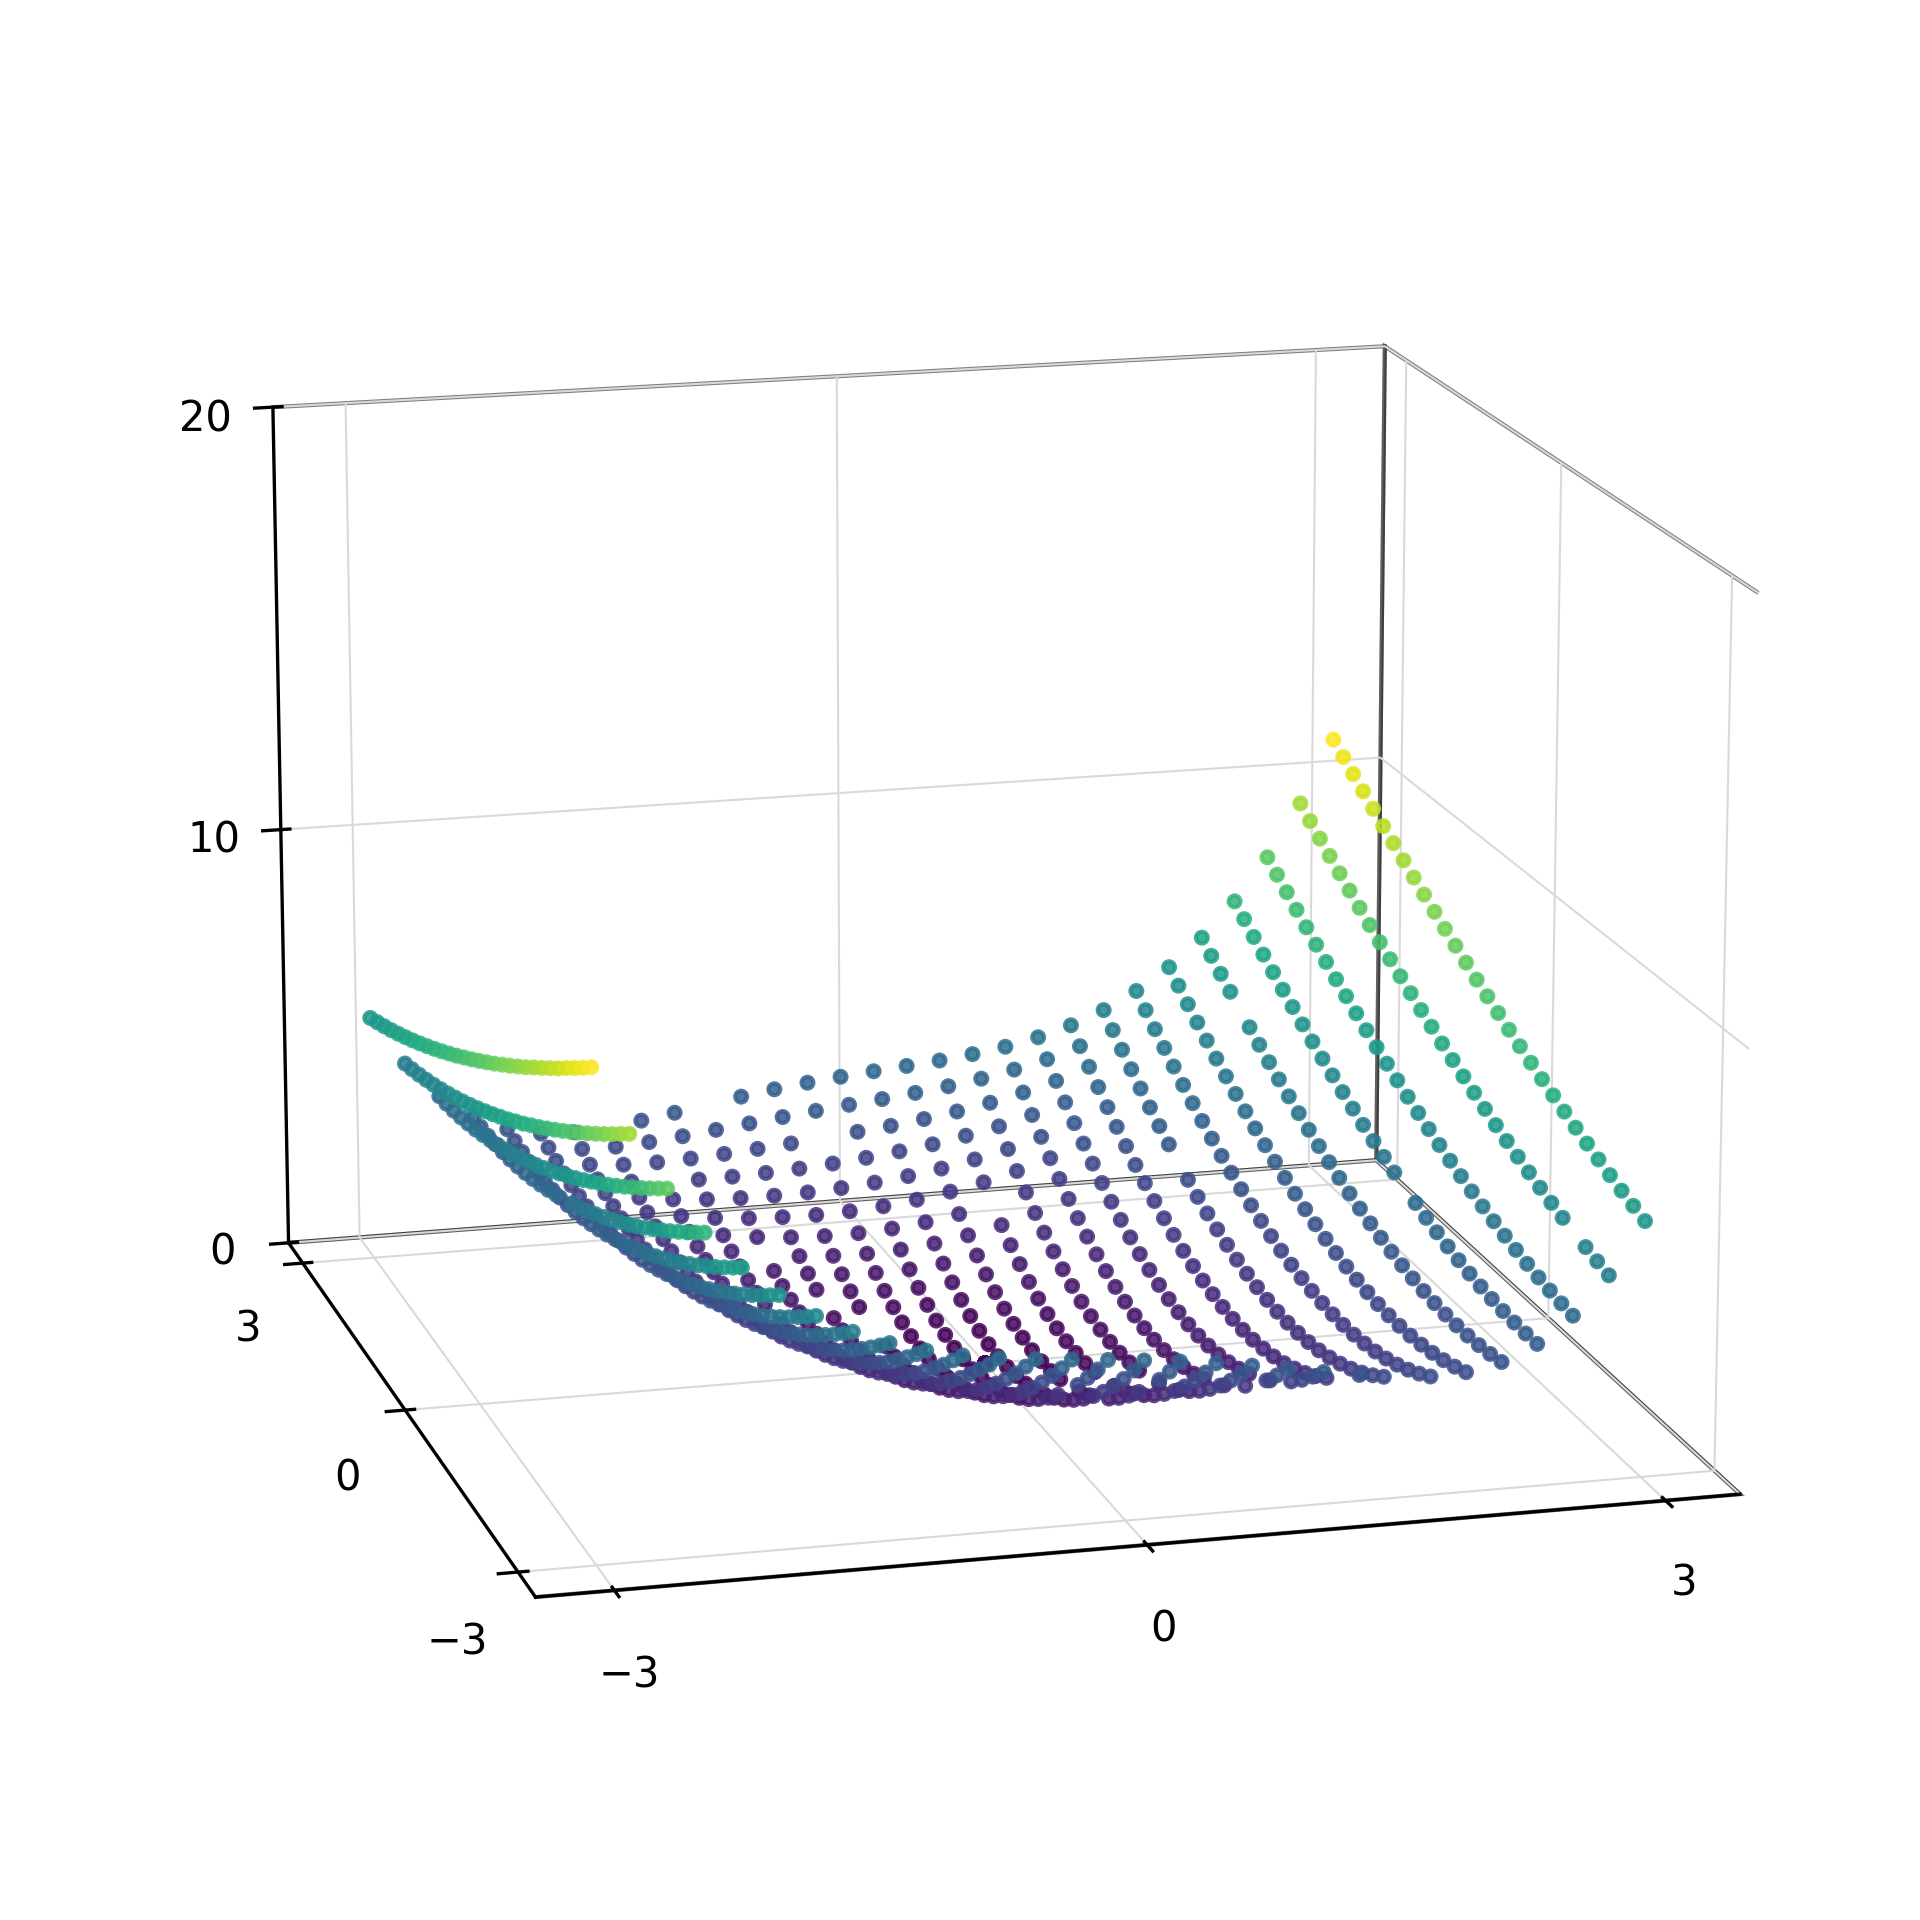
\includegraphics[width=0.48\textwidth]{plot/v.png}
\hfill
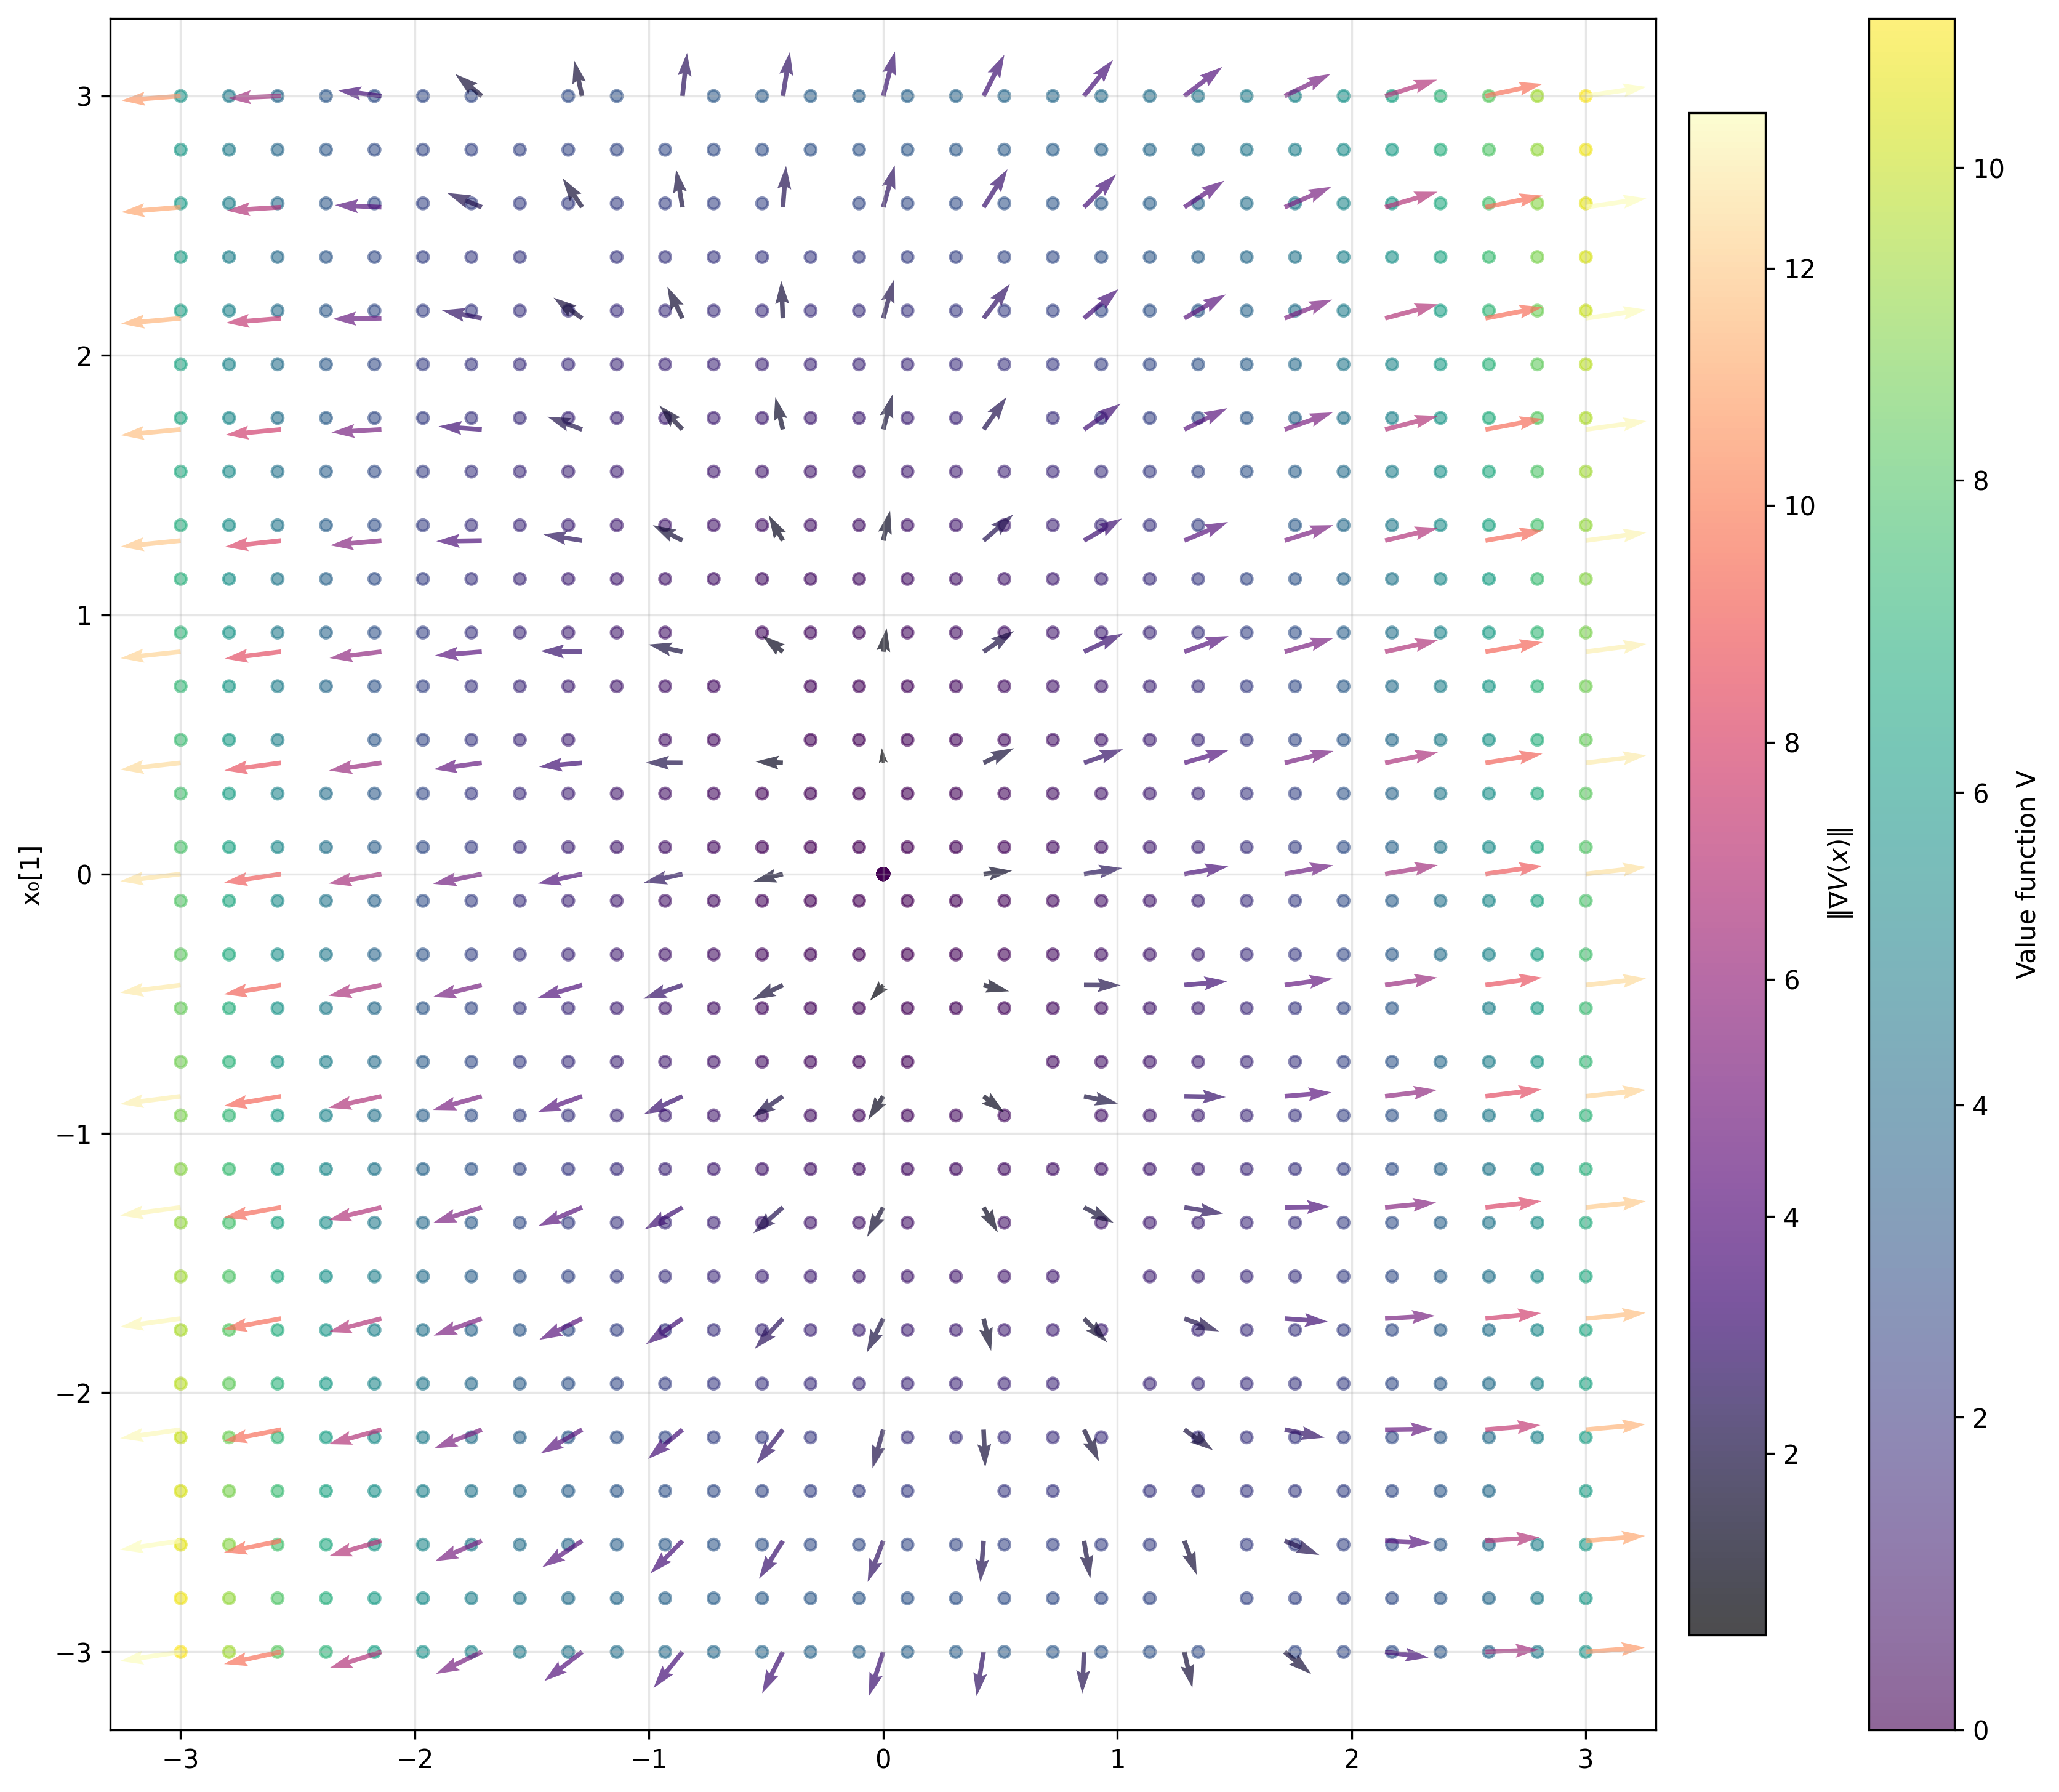
\includegraphics[width=0.48\textwidth]{plot/dv.png}
\caption{Left: value function $V(x)$ over $[-3,3]^2$. Right: $V(x)$ (dot
color) and costate labels $g^m$ (arrows); arrow color indicates $|g^m|$.}
\label{fig:vdp_data}
\end{figure}

All experiments use $T_{\mathrm{out}} = 150$ outer iterations and
$N_{\mathrm{trial}} = 50$ sampled candidate nodes per iteration. Each iteration
inserts the single selected candidate ($N_{\mathrm{ins}} = 1$), so the
one-candidate decrease statement applies. Corollary~\ref{cor:certificate-rate}
remains conditional on the selected
candidate being an exact global maximizer and is not claimed for the multistart
search. The loop terminates when no candidate clears the insertion threshold.

\subsubsection{Effect of the moment order \texorpdfstring{$p$}{p}}
\label{sec:effect-of-p}

The moment order enters the objective through the weight
$w_p(\omega)=1+|\omega|^p$ inside the scalar penalty: an atom at
$\omega$ is charged $\phi_\gamma\bigl(w_p(\omega)|c|\bigr)$ rather than
$\phi_\gamma(|c|)$, so a fixed coefficient becomes more expensive the further
the atom sits from the origin. The exponent $p$ is therefore an active
parameter of the objective, not a device that acts only through a separate
coefficient.

\paragraph{\textbf{Observed support radius.}}
For a finite atomic $\mu$ write
\begin{equation*}
	R_{\max}(\mu):=\max\{|\omega| : \omega\in\atom\mu\}
\end{equation*}
for the radius of its support. Lemma~\ref{lem:support-bound} places that
support in a compact superlevel set of $|\bar P_p|$, so $R_{\max}$ is finite;
the lemma does not itself supply a numerical radius, and the values below are
measured. We use Algorithm~\ref{alg:log} with
$\gamma=1$, equal value and gradient weights, and seed $42$, for softplus,
$\tanh$, the Gaussian and $\mathrm{GELU}^2$, over
\begin{equation*}
	\alpha\in\{10^{-4},10^{-5}\},
	\qquad
	p\in\{2.01,2.5,3,4\},
\end{equation*}
on both benchmarks. Figure~\ref{fig:p_study} shows the resulting sixteen
(problem, activation, $\alpha$) families. In every family $R_{\max}$ decreases
monotonically over the tested orders. The largest contraction is for
$\mathrm{GELU}^2$ on the pendulum at $\alpha=10^{-5}$, from $148.06$ at
$p=2.01$ to $6.77$ at $p=4$; across all families the largest radius at $p=4$
is $11.99$.

We also record the radius $R_{0.95}$, defined for a discrete
measure $\mu=\sum_jc_j\delta_{\omega_j}$ by
\begin{equation*}
	R_{0.95}(\mu):=\inf\left\{R\ge0:
	|\mu|(B_R)\ge0.95\,|\mu|(\Omega)\right\},
\end{equation*}
and the support size $N$. Unlike $R_{\max}$, both depend on the fitted
coefficient distribution. Each decreases monotonically in twelve of the
sixteen families, rather than all sixteen, so their behavior is reported
separately rather than inferred from the support theorem.

\begin{figure}[htbp]
\centering
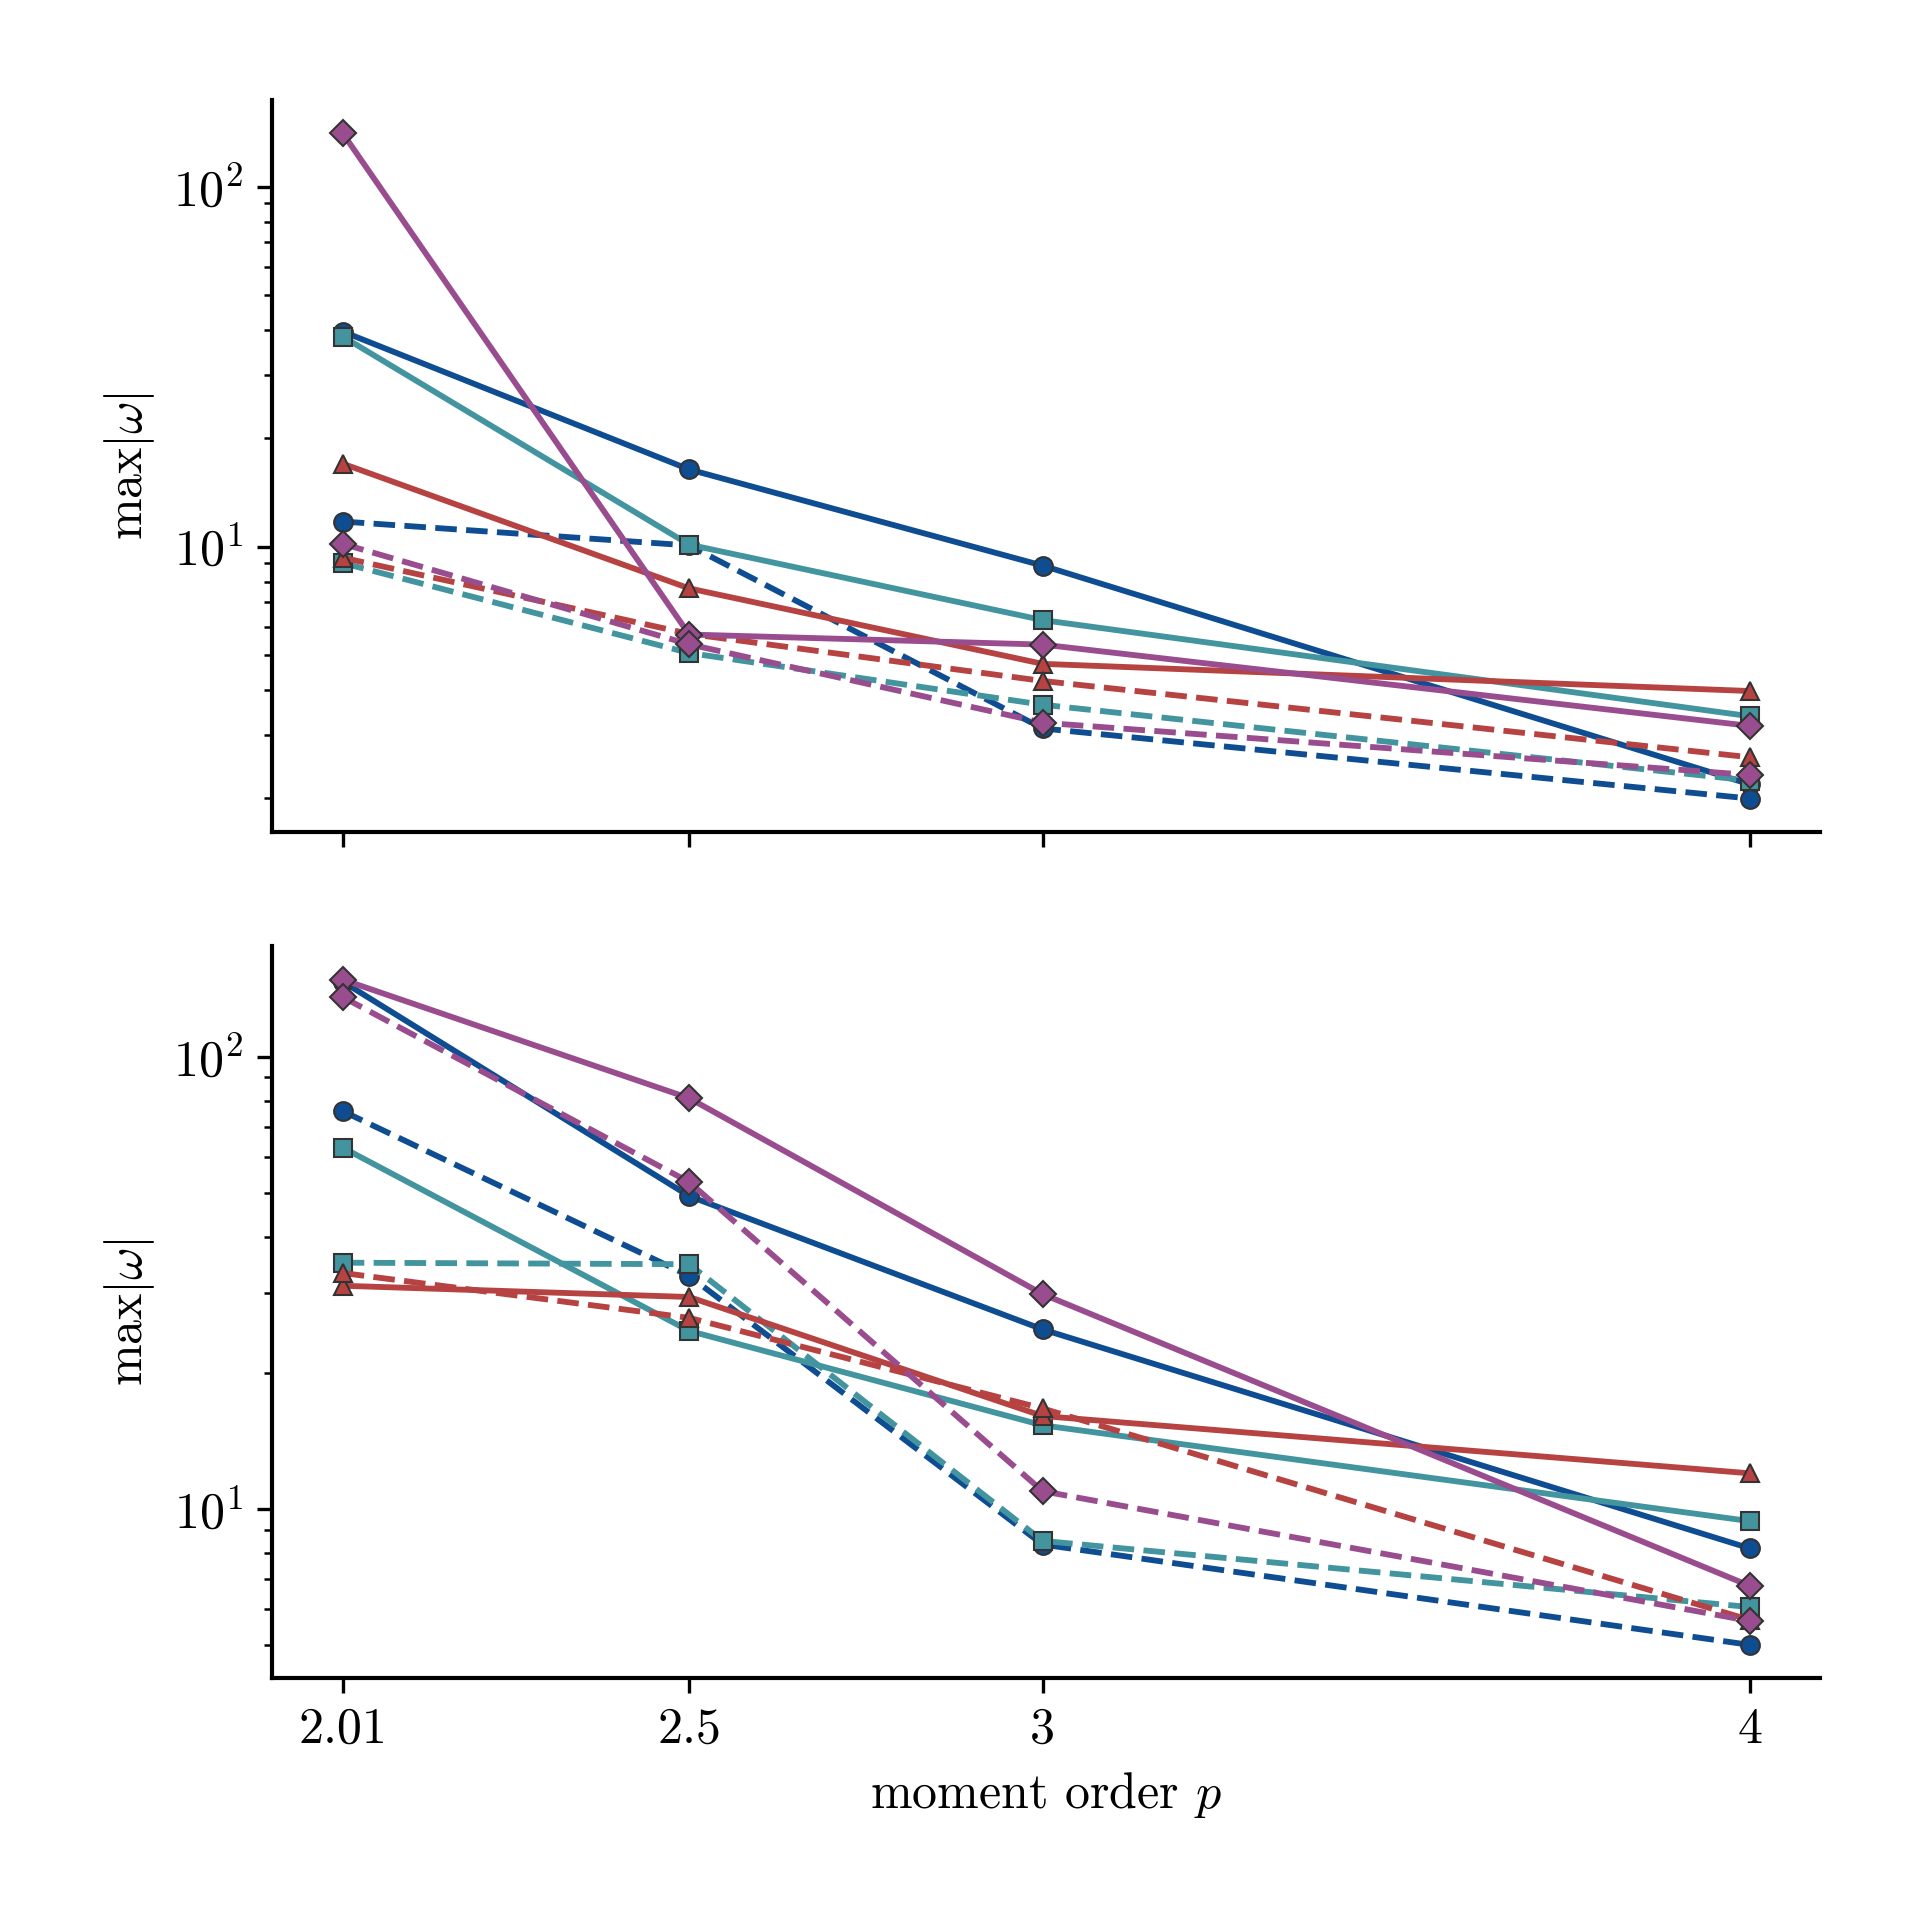
\includegraphics[width=0.8\textwidth]{../experiments/01_vdp/paper_log_penalty/figures/p_study.png}
\caption{Support radius $R_{\max}$ against the moment order $p$, for softplus,
$\tanh$, the Gaussian and $\mathrm{GELU}^2$ at $\alpha=10^{-4}$ and
$\alpha=10^{-5}$; upper panel Van der Pol, lower panel pendulum swing-up.
Colour identifies the activation and line style the value of $\alpha$. All
sixteen support-radius curves decrease monotonically; all use seed $42$.}
\label{fig:p_study}
\end{figure}

\paragraph{\textbf{The computable search radius.}}
Theorem~\ref{thm:quantitative-insertion} supplies the radius
\eqref{eq:explicit-certificate-radius} outside which no candidate can satisfy
the insertion condition. Its constants are available before the fit: the
growth exponents $s_0,s_1$ and the constant $C_\rho$ of
Assumption~\ref{ass:value-growth} are properties of the activation, and the
remaining factor follows from the sample extent, so
$C=C_\rho\bigl(A_M^{s_0}+A_M^{s_1-1}\bigr)$ with
$A_M=\max\{1,\max_m\sqrt{1+|x^m|^2}\}$. Nothing is calibrated from the fit.

On the Van der Pol data ($A_M=\sqrt3$, hence $C=2.73$ for softplus) the radius
is $56.5$ at $p=4$, $\alpha=10^{-4}$ and $121.7$ at $p=4$, $\alpha=10^{-5}$,
while for $p\le3$ it exceeds the implementation's own bound $\lambda\le e^5$.
The radius is therefore informative only at the largest tested $p$, and only
for the activations with $s_1=1$; for $\mathrm{GELU}^2$, where $s_1=2$, the
exponent $1/(p-s_1)$ never becomes small enough on this grid.

The fixed-versus-theorem ablation shows a small but nonzero effect. Among the
thirty-two paired sequential-insertion Van der Pol runs, eight change when
$\min\{R(\mu_t),e^5\}$ replaces the fixed $e^5$ search filter: two at $p=3$
and six at $p=4$. The relative $H^1$ differences are at most
$2.8\times10^{-3}$, and their sign is mixed. Because the radius determines
both the distribution of random starts and the admissible final candidates,
the change does not require a retained atom to sit on the boundary. The
computable radius becomes operational only at the largest moment orders on
this grid; it does not systematically improve or degrade the fit.

\subsubsection{Algorithm~\ref{alg:log}: the log penalty on the normalized measure}

We investigate the effect of including gradient data for softplus, $\tanh$,
and the Gaussian. Table~\ref{tab:alg1_gradient} compares fitting the values
alone with fitting both values and gradients.

\begin{table}[htbp]
\centering
\caption{Effect of gradient-augmented fitting with
$\alpha=10^{-4}$, $\gamma=10$, $p=2.01$, seed $42$. The same parameters are
used for all three activations, so the comparison is not confounded with
per-activation tuning.}
\label{tab:alg1_gradient}
\begin{subtable}{0.48\textwidth}
\centering
\setlength{\tabcolsep}{9pt}
\renewcommand{\arraystretch}{1.25}
\begin{tabular}{lcc}
\toprule
Activation & $L^2$ trained & $H^1$ trained \\
\midrule
softplus & $1.04 \times 10^{-1}$ & $4.24 \times 10^{-1}$ \\
tanh & $9.58 \times 10^{-2}$ & $4.17 \times 10^{-1}$ \\
Gaussian & $7.16 \times 10^{-2}$ & $4.17 \times 10^{-1}$ \\
\bottomrule
\end{tabular}
\caption{Effect of gradient training on $\mathrm{Err}_{L^2}$ }
\label{tab:alg1_gradient_errl2}
\end{subtable}
\hfill
\begin{subtable}{0.48\textwidth}
\centering
\setlength{\tabcolsep}{9pt}
\renewcommand{\arraystretch}{1.25}
\begin{tabular}{lcc}
\toprule
Activation & $L^2$ trained & $H^1$ trained \\
\midrule
softplus & $5.82 \times 10^{-1}$ & $1.03 \times 10^{-1}$ \\
tanh & $5.97 \times 10^{-1}$ & $1.01 \times 10^{-1}$ \\
Gaussian & $5.37 \times 10^{-1}$ & $9.83 \times 10^{-2}$ \\
\bottomrule
\end{tabular}
\caption{Effect of gradient training on $\mathrm{Err}_{H^1}$}
\label{tab:alg1_gradient_errh1}
\end{subtable}
\end{table}

\paragraph{\textbf{Choice of activation function in gradient training.}}
We compare softplus, $\tanh$, and the Gaussian. Because the
gradient-augmented loss contains both the value and gradient errors,
$K(\omega)$ contributes to the approximation of $V$ and
$\nabla K(\omega)$ contributes to the approximation of $\nabla V$.
Figure~\ref{fig:activation_shapes} contrasts the three activations through
their value, first derivative, and second derivative.
The softplus derivative increases from $0$ to $1$, the derivative of $\tanh$
tends to zero at both ends of the real line, and the Gaussian derivative is
localized and changes sign. These derivatives generate different columns
$a\,\rho'(a\cdot x+b)$ in the gradient fitting problem.

\begin{figure}[htbp]
\centering
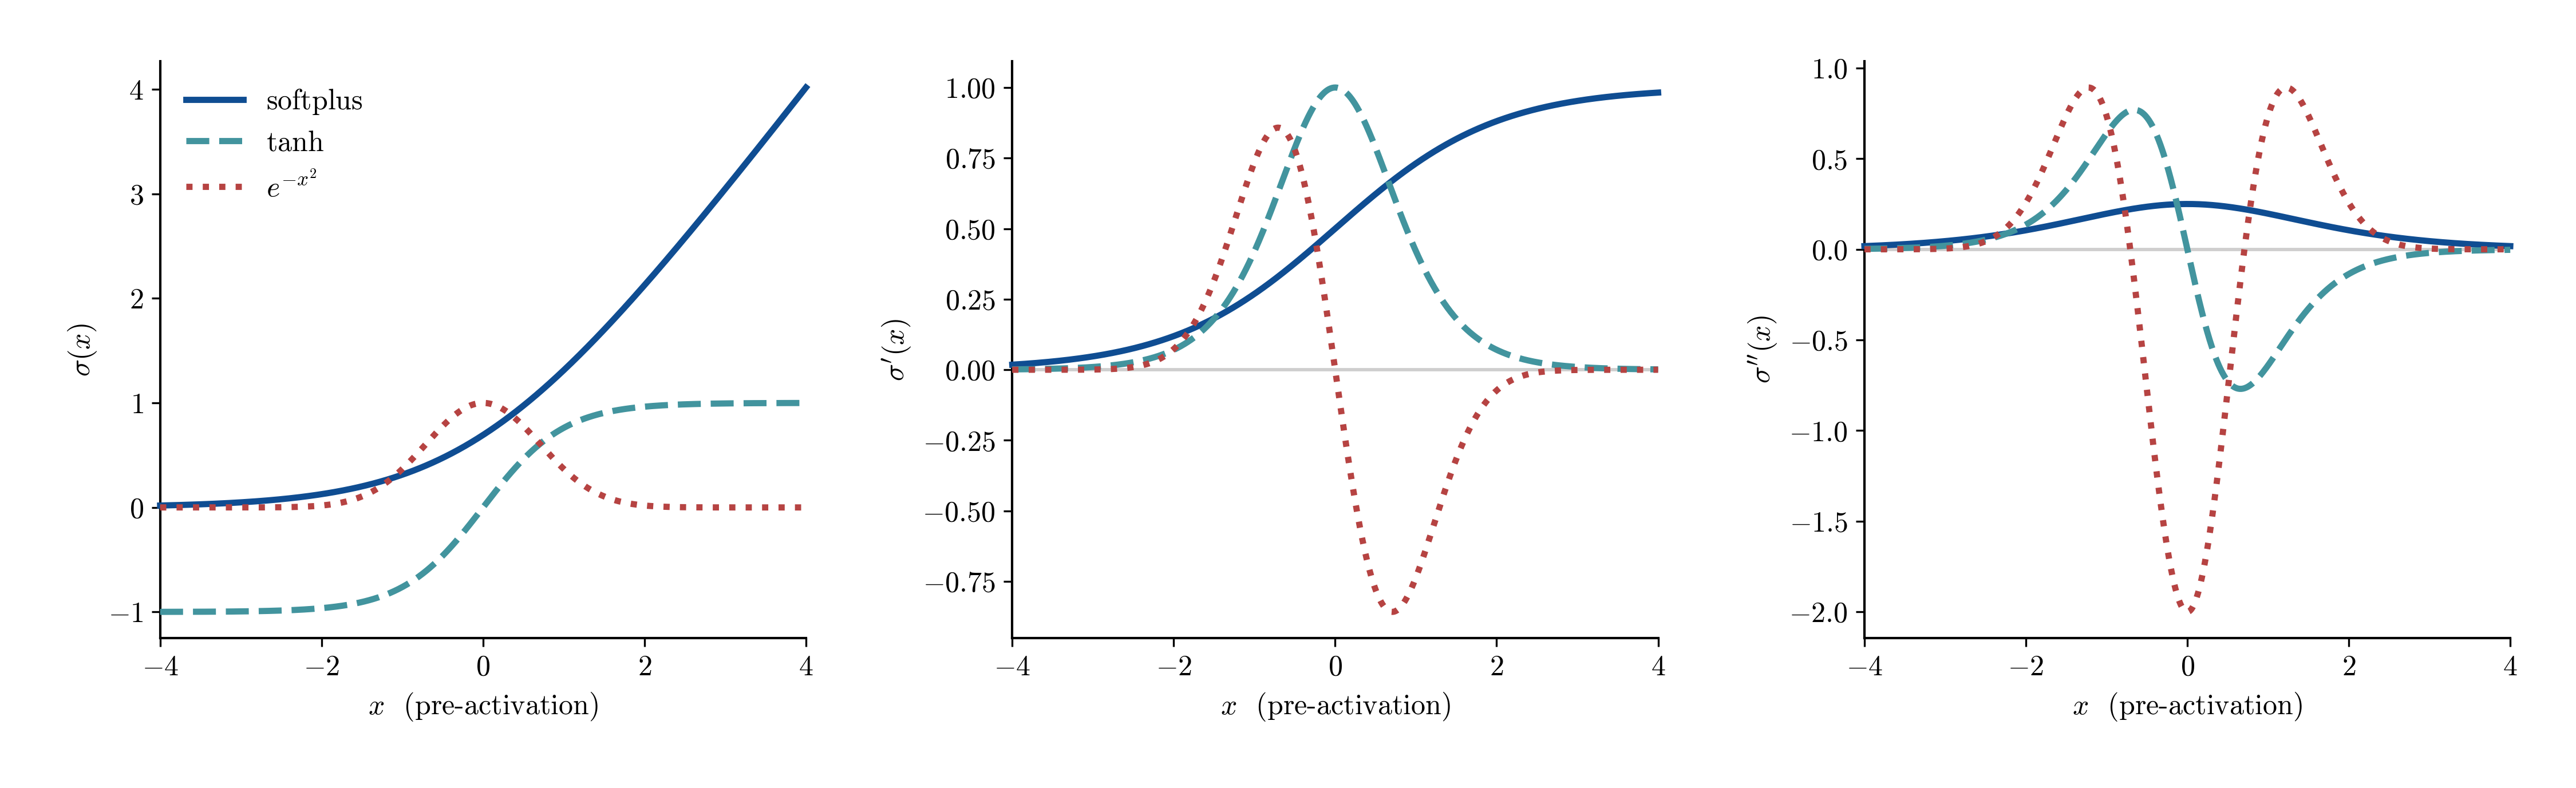
\includegraphics[width=\textwidth]{../experiments/01_vdp/paper_log_penalty/figures/shape_softplus_tanh_gaussian.png}
\caption{The three smooth profiles used by Algorithm~\ref{alg:log} --- softplus,
$\tanh$, and the Gaussian $e^{-z^2}$ --- shown as $\rho$, $\rho'$, and
$\rho''$. Under the gradient-augmented loss,
the first derivative is the basis that reconstructs $\nabla V$.}
\label{fig:activation_shapes}
\end{figure}

For the tested parameters, the Gaussian has the smallest relative $H^1$ error.
All three approximate the smooth value function, with different support sizes.

\begin{figure}[htbp]
\centering
\captionsetup[subfigure]{justification=centering}
\begin{subfigure}[t]{0.32\textwidth}
\centering
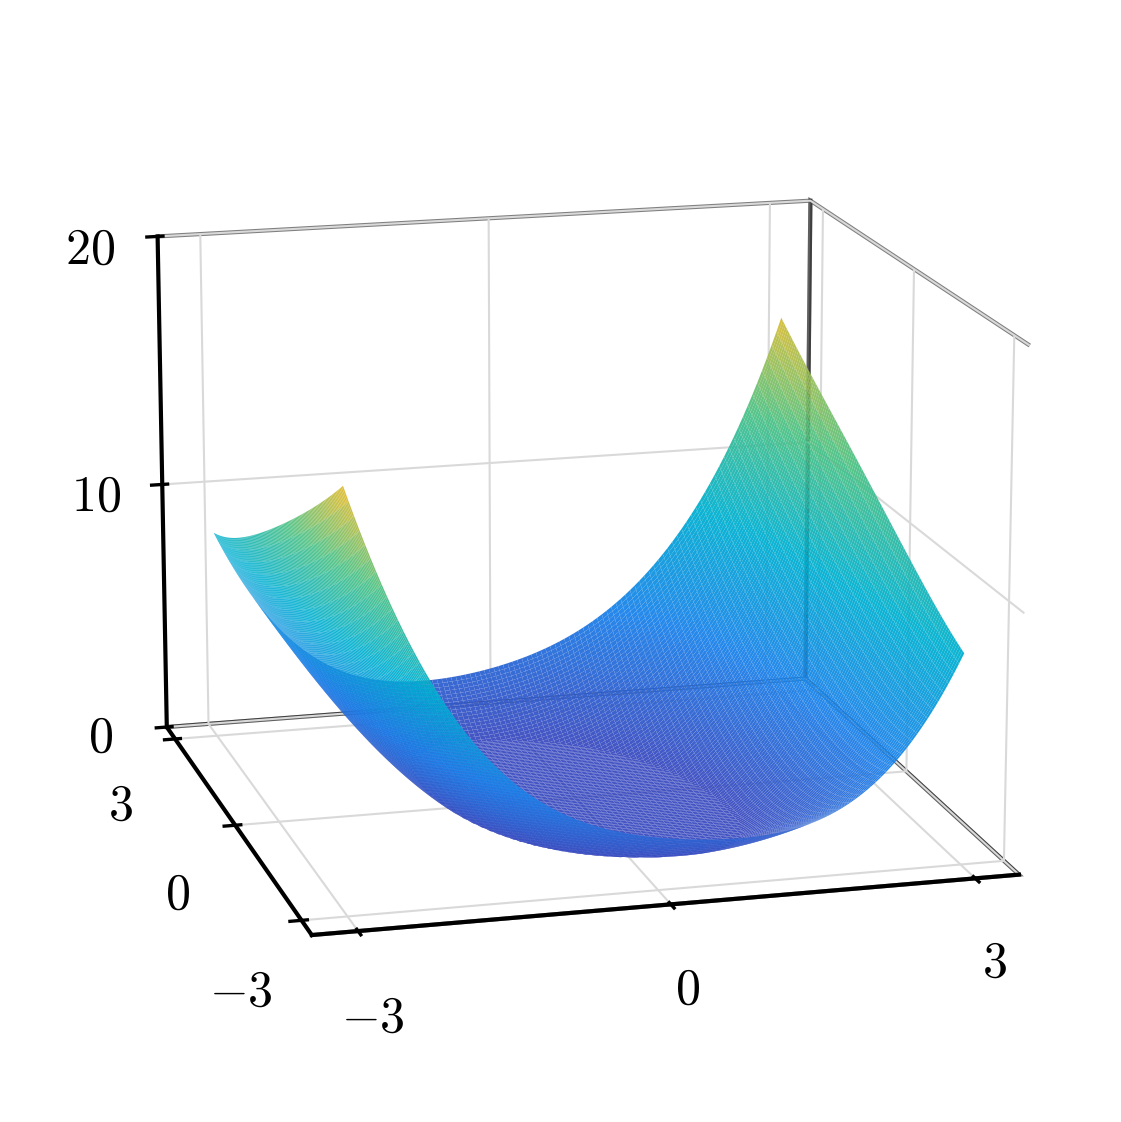
\includegraphics[width=\textwidth]{../experiments/01_vdp/paper_log_penalty/figures/value_surface_softplus.png}
\caption{softplus\\ ($N=16$, $\mathrm{Err}_{H^1} = 0.103$).}
\label{fig:h1_activation_softplus}
\end{subfigure}
\hfill
\begin{subfigure}[t]{0.32\textwidth}
\centering
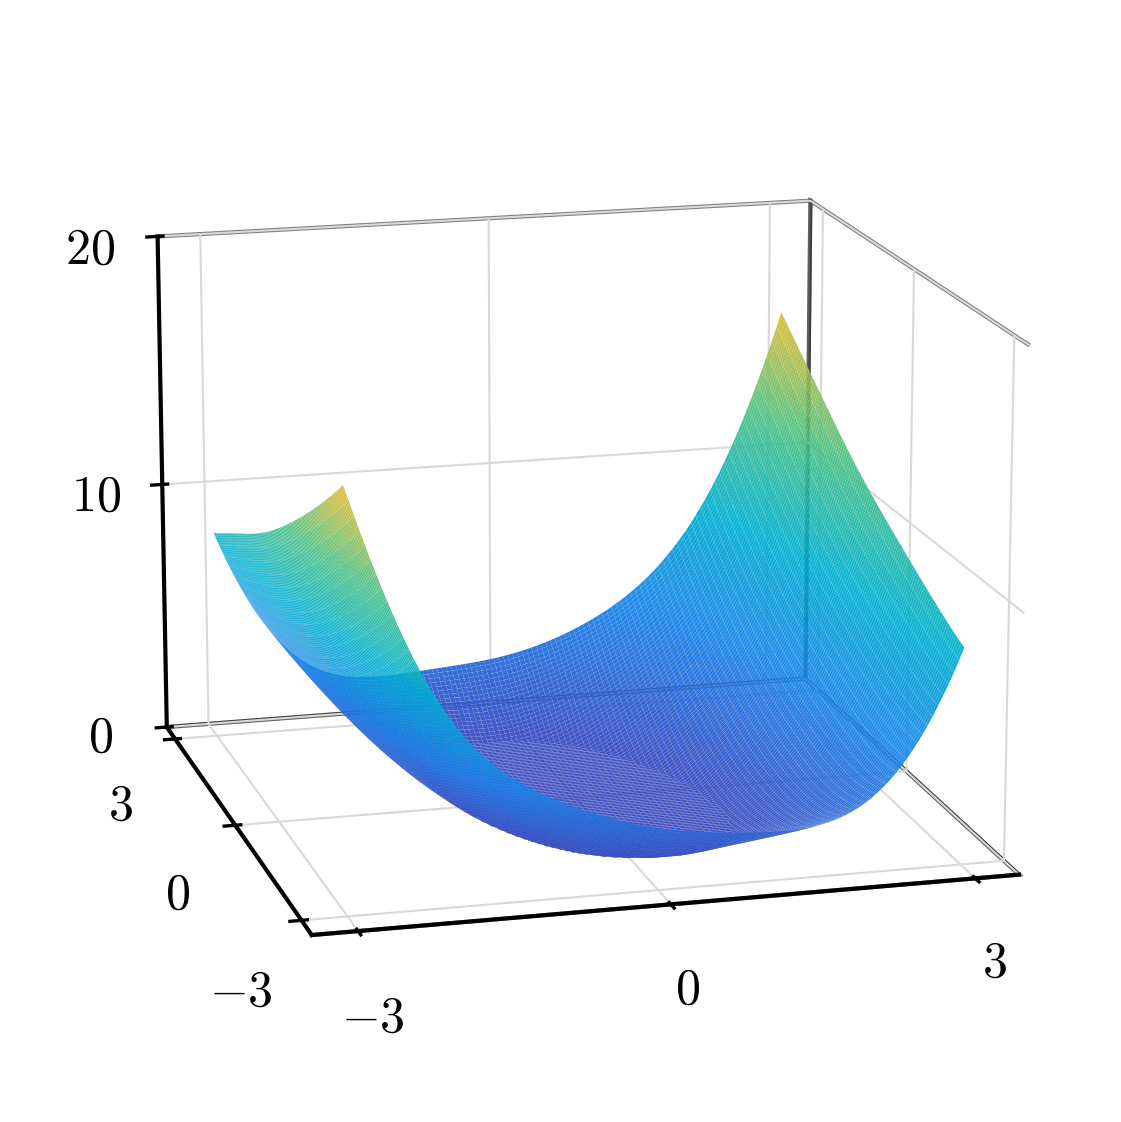
\includegraphics[width=\textwidth]{../experiments/01_vdp/paper_log_penalty/figures/value_surface_tanh.png}
\caption{$\tanh$\\ ($N=38$, $\mathrm{Err}_{H^1} = 0.101$).}
\label{fig:h1_activation_tanh}
\end{subfigure}
\hfill
\begin{subfigure}[t]{0.32\textwidth}
\centering
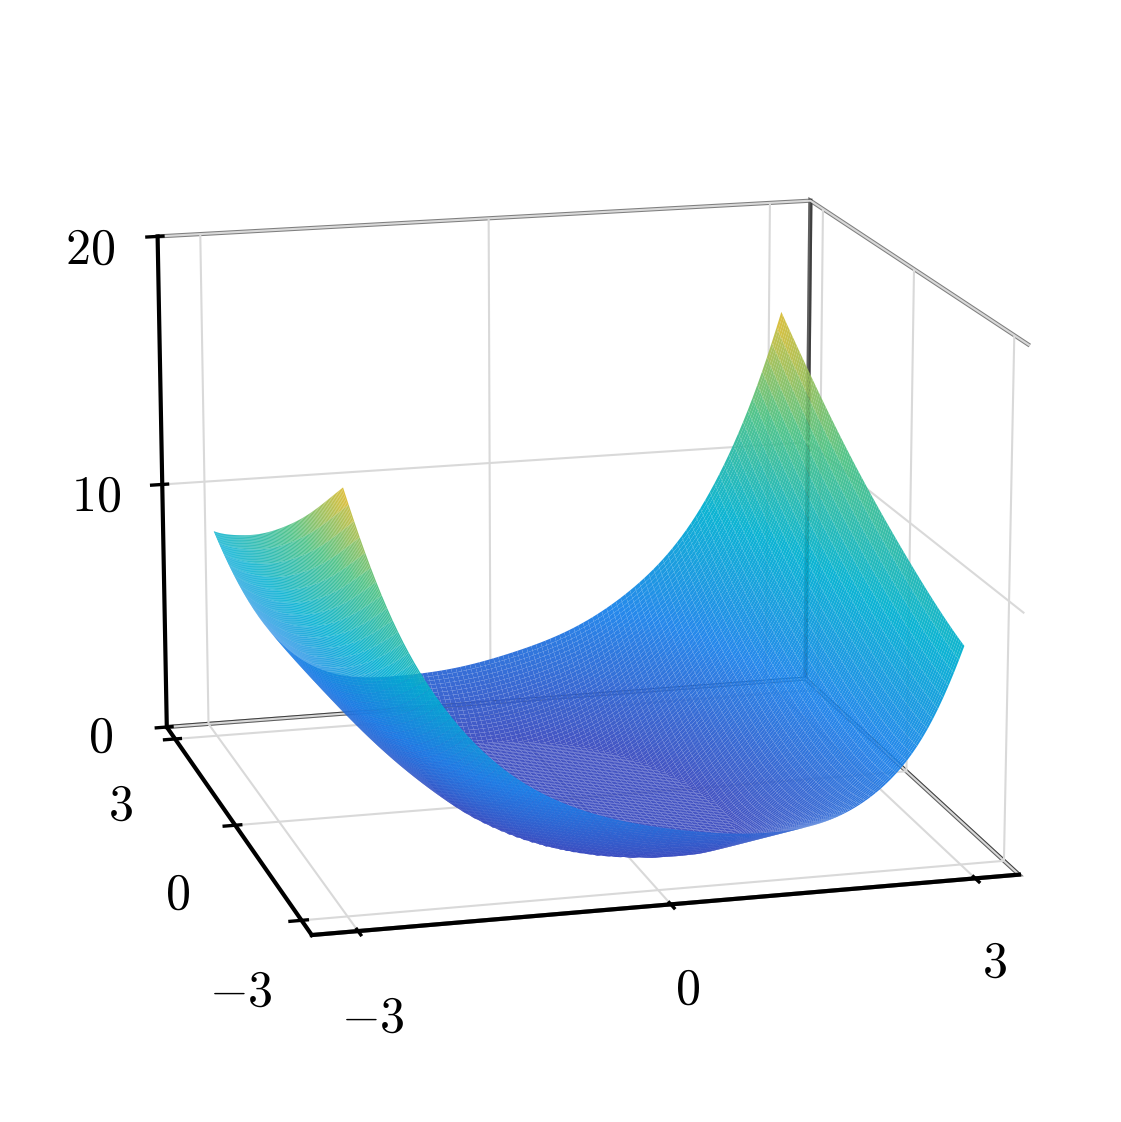
\includegraphics[width=\textwidth]{../experiments/01_vdp/paper_log_penalty/figures/value_surface_gaussian.png}
\caption{Gaussian\\ ($N=34$, $\mathrm{Err}_{H^1} = 0.098$).}
\label{fig:h1_activation_gaussian}
\end{subfigure}
\caption{Learned value functions under the $H^1$ loss using the parameter
values in Table~\ref{tab:alg1_gradient}. All three
approximate the smooth value surface; they differ in support size and
accuracy.}
\label{fig:h1_activation}
\end{figure}

\begin{table}[htbp]
\centering
\caption{Support size and validation error for the parameter values in
Table~\ref{tab:alg1_gradient}.}
\label{tab:alg1_sparsity}
\begin{subtable}{0.48\textwidth}
\centering
\setlength{\tabcolsep}{12pt}
\renewcommand{\arraystretch}{1.25}
\begin{tabular}{lcc}
\toprule
Activation & $N$ & $\mathrm{Err}_{L^2}$ \\
\midrule
softplus & 6 & $1.04 \times 10^{-1}$ \\
tanh & 10 & $9.58 \times 10^{-2}$ \\
Gaussian & 10 & $7.16 \times 10^{-2}$ \\
\bottomrule
\end{tabular}
\caption{$L^2$ trained}
\label{tab:alg1_sparsity_l2}
\end{subtable}
\hfill
\begin{subtable}{0.48\textwidth}
\centering
\setlength{\tabcolsep}{12pt}
\renewcommand{\arraystretch}{1.25}
\begin{tabular}{lcc}
\toprule
Activation & $N$ & $\mathrm{Err}_{H^1}$ \\
\midrule
softplus & 16 & $1.03 \times 10^{-1}$ \\
tanh & 38 & $1.01 \times 10^{-1}$ \\
Gaussian & 34 & $9.83 \times 10^{-2}$ \\
\bottomrule
\end{tabular}
\caption{$H^1$ trained}
\label{tab:alg1_sparsity_h1}
\end{subtable}
\end{table}

With the $H^1$ loss, all three gradient errors fall substantially: from
$5.96\times10^{-1}$ to $4.36\times10^{-2}$ for softplus, from
$6.12\times10^{-1}$ to $4.22\times10^{-2}$ for $\tanh$, and from
$5.51\times10^{-1}$ to $3.57\times10^{-2}$ for the Gaussian. Fitting values
alone leaves the gradient essentially unapproximated, and the resulting
feedback law would be unusable.

The Gaussian is most accurate ($9.83\times10^{-2}$) and uses $34$ atoms;
$\tanh$ reaches $1.01\times10^{-1}$ with $38$, and softplus
$1.03\times10^{-1}$ with only $16$. The three are separated by less in
accuracy than in support size, so the ordering by
$\mathrm{Err}_{H^1}$ alone understates the difference between them.

\subsubsection{Algorithm~\ref{alg:q}: $|c|^q$-penalty with $\reluk$ activation}

Algorithm~\ref{alg:q} uses the profile
$\rho(z)=\mathrm{ReLU}(z)^k$ with the penalty $\psi_k$, namely
$\alpha \sum_i |c_i|^q$ with $q = 2/(k+1)$.
The swept parameter is the power $k$; all fits below use
$\alpha = 10^{-5}$.


\begin{figure}[htbp]
\centering
\captionsetup[subfigure]{justification=centering}
\begin{subfigure}[t]{0.48\textwidth}
\centering
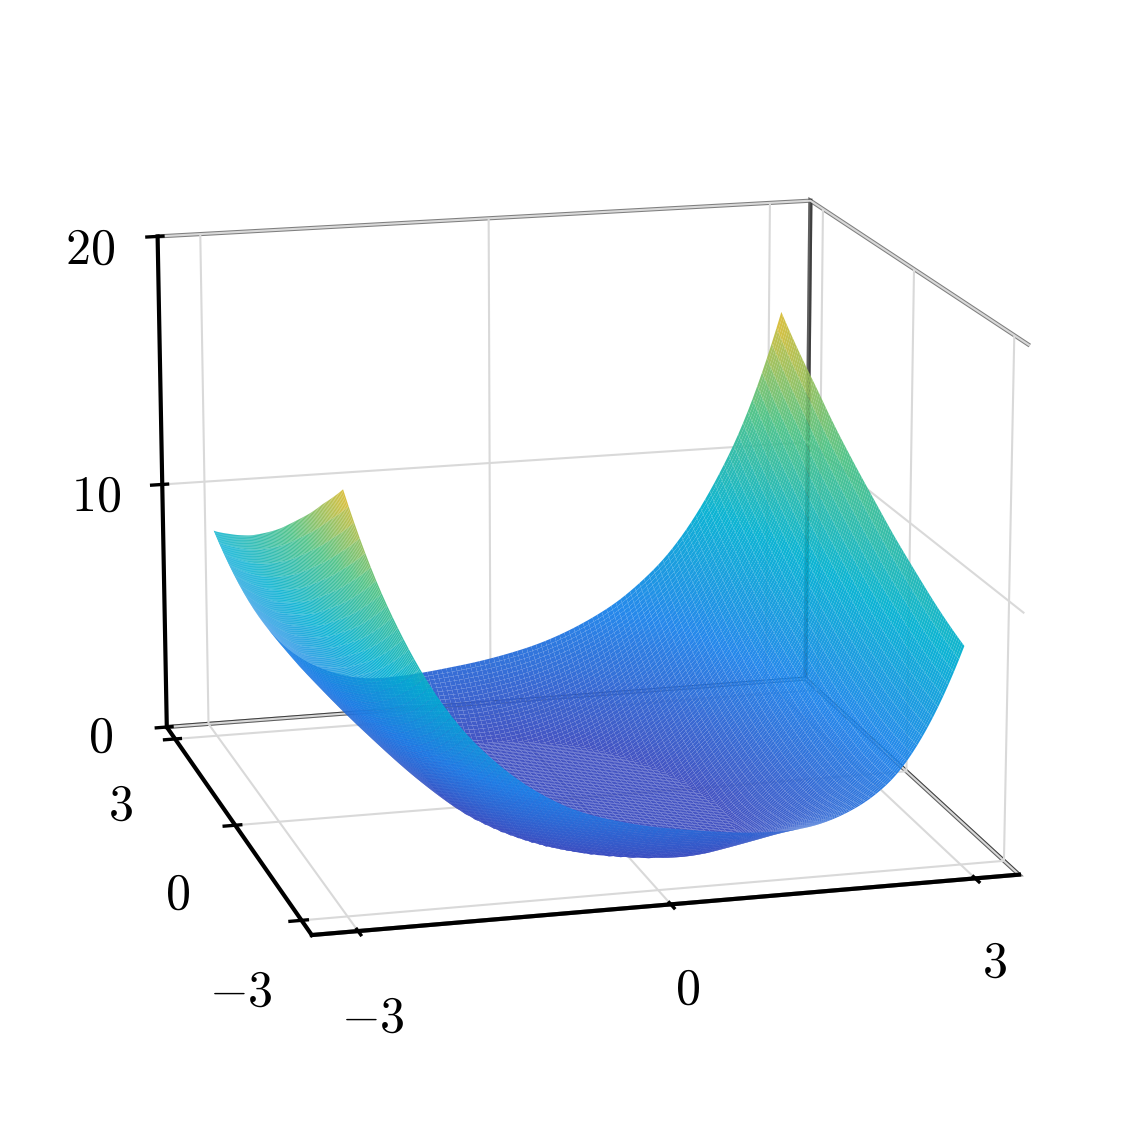
\includegraphics[width=\textwidth]{../experiments/01_vdp/paper_frac_exp_penalty/figures/value_surface_p2.png}
\caption{$k=2$\\ ($N=45$, $\mathrm{Err}_{H^1} = 0.099$).}
\label{fig:H1_power_p2}
\end{subfigure}
\hfill
\begin{subfigure}[t]{0.48\textwidth}
\centering
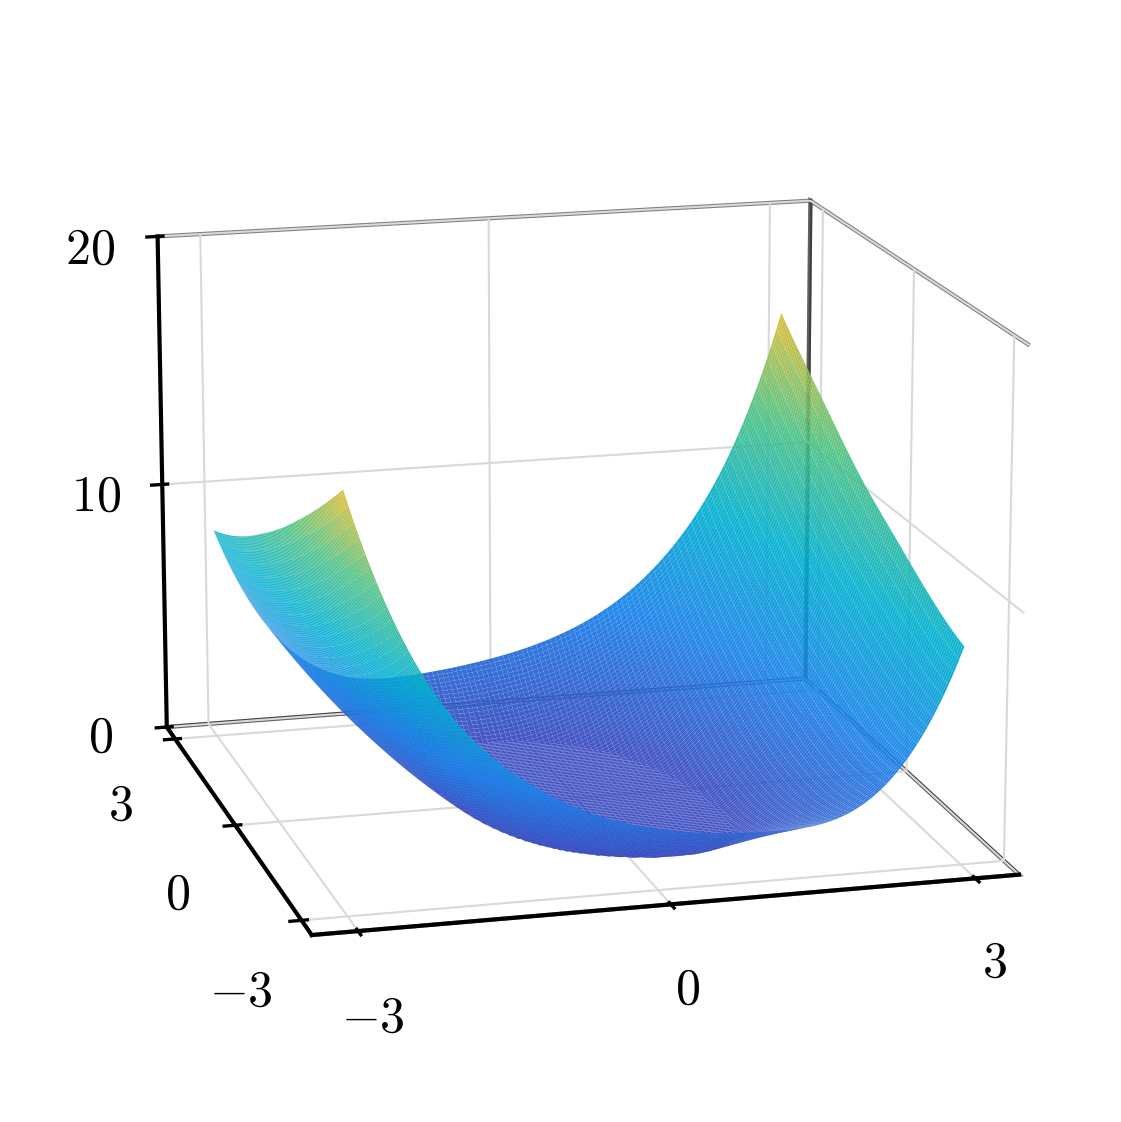
\includegraphics[width=\textwidth]{../experiments/01_vdp/paper_frac_exp_penalty/figures/value_surface_p3.png}
\caption{$k=3$\\ ($N=28$, $\mathrm{Err}_{H^1} = 0.099$).}
\label{fig:H1_power_p3}
\end{subfigure}
\caption{$H^1$-trained networks with $\alpha = 10^{-5}$ for
$k \in \{2,3\}$.}
\label{fig:H1_power}
\end{figure}

Under the $L^2$ loss the gradient error stays large for both powers
($\mathrm{Err}_{H^1} \approx 4$--$5 \times 10^{-1}$): the value-only fit
ignores $\nabla V$, so the atoms are placed without regard to the gradient
field. The $H^1$ loss drives the gradient error down to
$\approx 1.0 \times 10^{-1}$ for both powers
(Table~\ref{tab:alg2_gradient}).

\begin{table}[htbp]
\centering
\caption{Algorithm~2: network size and validation error vs.\ the atom power $k$ ($\alpha = 10^{-5}$).}
\label{tab:alg2_gradient}
\begin{subtable}{0.48\textwidth}
\centering
\setlength{\tabcolsep}{6pt}
\renewcommand{\arraystretch}{1.25}
\begin{tabular}{lccc}
\toprule
Power & $N$ & $\mathrm{Err}_{L^2}$ & $\mathrm{Err}_{H^1}$ \\
\midrule
$k = 2$ & 13 & $2.78 \times 10^{-2}$ & $4.09 \times 10^{-1}$ \\
$k = 3$ & 13 & $2.61 \times 10^{-2}$ & $4.18 \times 10^{-1}$ \\
\bottomrule
\end{tabular}
\caption{$L^2$ trained}
\label{tab:alg2_gradient_l2}
\end{subtable}
\hfill
\begin{subtable}{0.48\textwidth}
\centering
\setlength{\tabcolsep}{6pt}
\renewcommand{\arraystretch}{1.25}
\begin{tabular}{lccc}
\toprule
Power & $N$ & $\mathrm{Err}_{L^2}$ & $\mathrm{Err}_{H^1}$ \\
\midrule
$k = 2$ & 45 & $4.17 \times 10^{-1}$ & $9.85 \times 10^{-2}$ \\
$k = 3$ & 28 & $4.15 \times 10^{-1}$ & $9.86 \times 10^{-2}$ \\
\bottomrule
\end{tabular}
\caption{$H^1$ trained}
\label{tab:alg2_gradient_h1}
\end{subtable}
\end{table}

Changing $k$ changes both the activation and the induced exponent
$q=2/(k+1)$. At the same $H^1$ error scale, the $k=3$ fit uses $28$ atoms
instead of $45$ for $k=2$.
Under the $L^2$ loss both fits use $13$ atoms and have
$\mathrm{Err}_{H^1} \approx 4.1$--$4.2 \times 10^{-1}$
(Table~\ref{tab:alg2_gradient}\,(a)).

\subsubsection{Summary}

Figure~\ref{fig:summary_frontier} plots the running best relative $H^1$ error
along the selected fits. At the shared Algorithm~1 operating point, softplus
uses $16$ atoms at error $1.03\times10^{-1}$ and the Gaussian uses $34$ at
$9.83\times10^{-2}$. The lowest-error Algorithm~2 checkpoints use $91$ atoms
at $9.83\times10^{-2}$ for $\mathrm{ReLU}^2$ and $37$ atoms at
$9.72\times10^{-2}$ for $\mathrm{ReLU}^3$. Thus all four reach the same
accuracy scale, with different support sizes.
\begin{figure}[htbp]
\centering
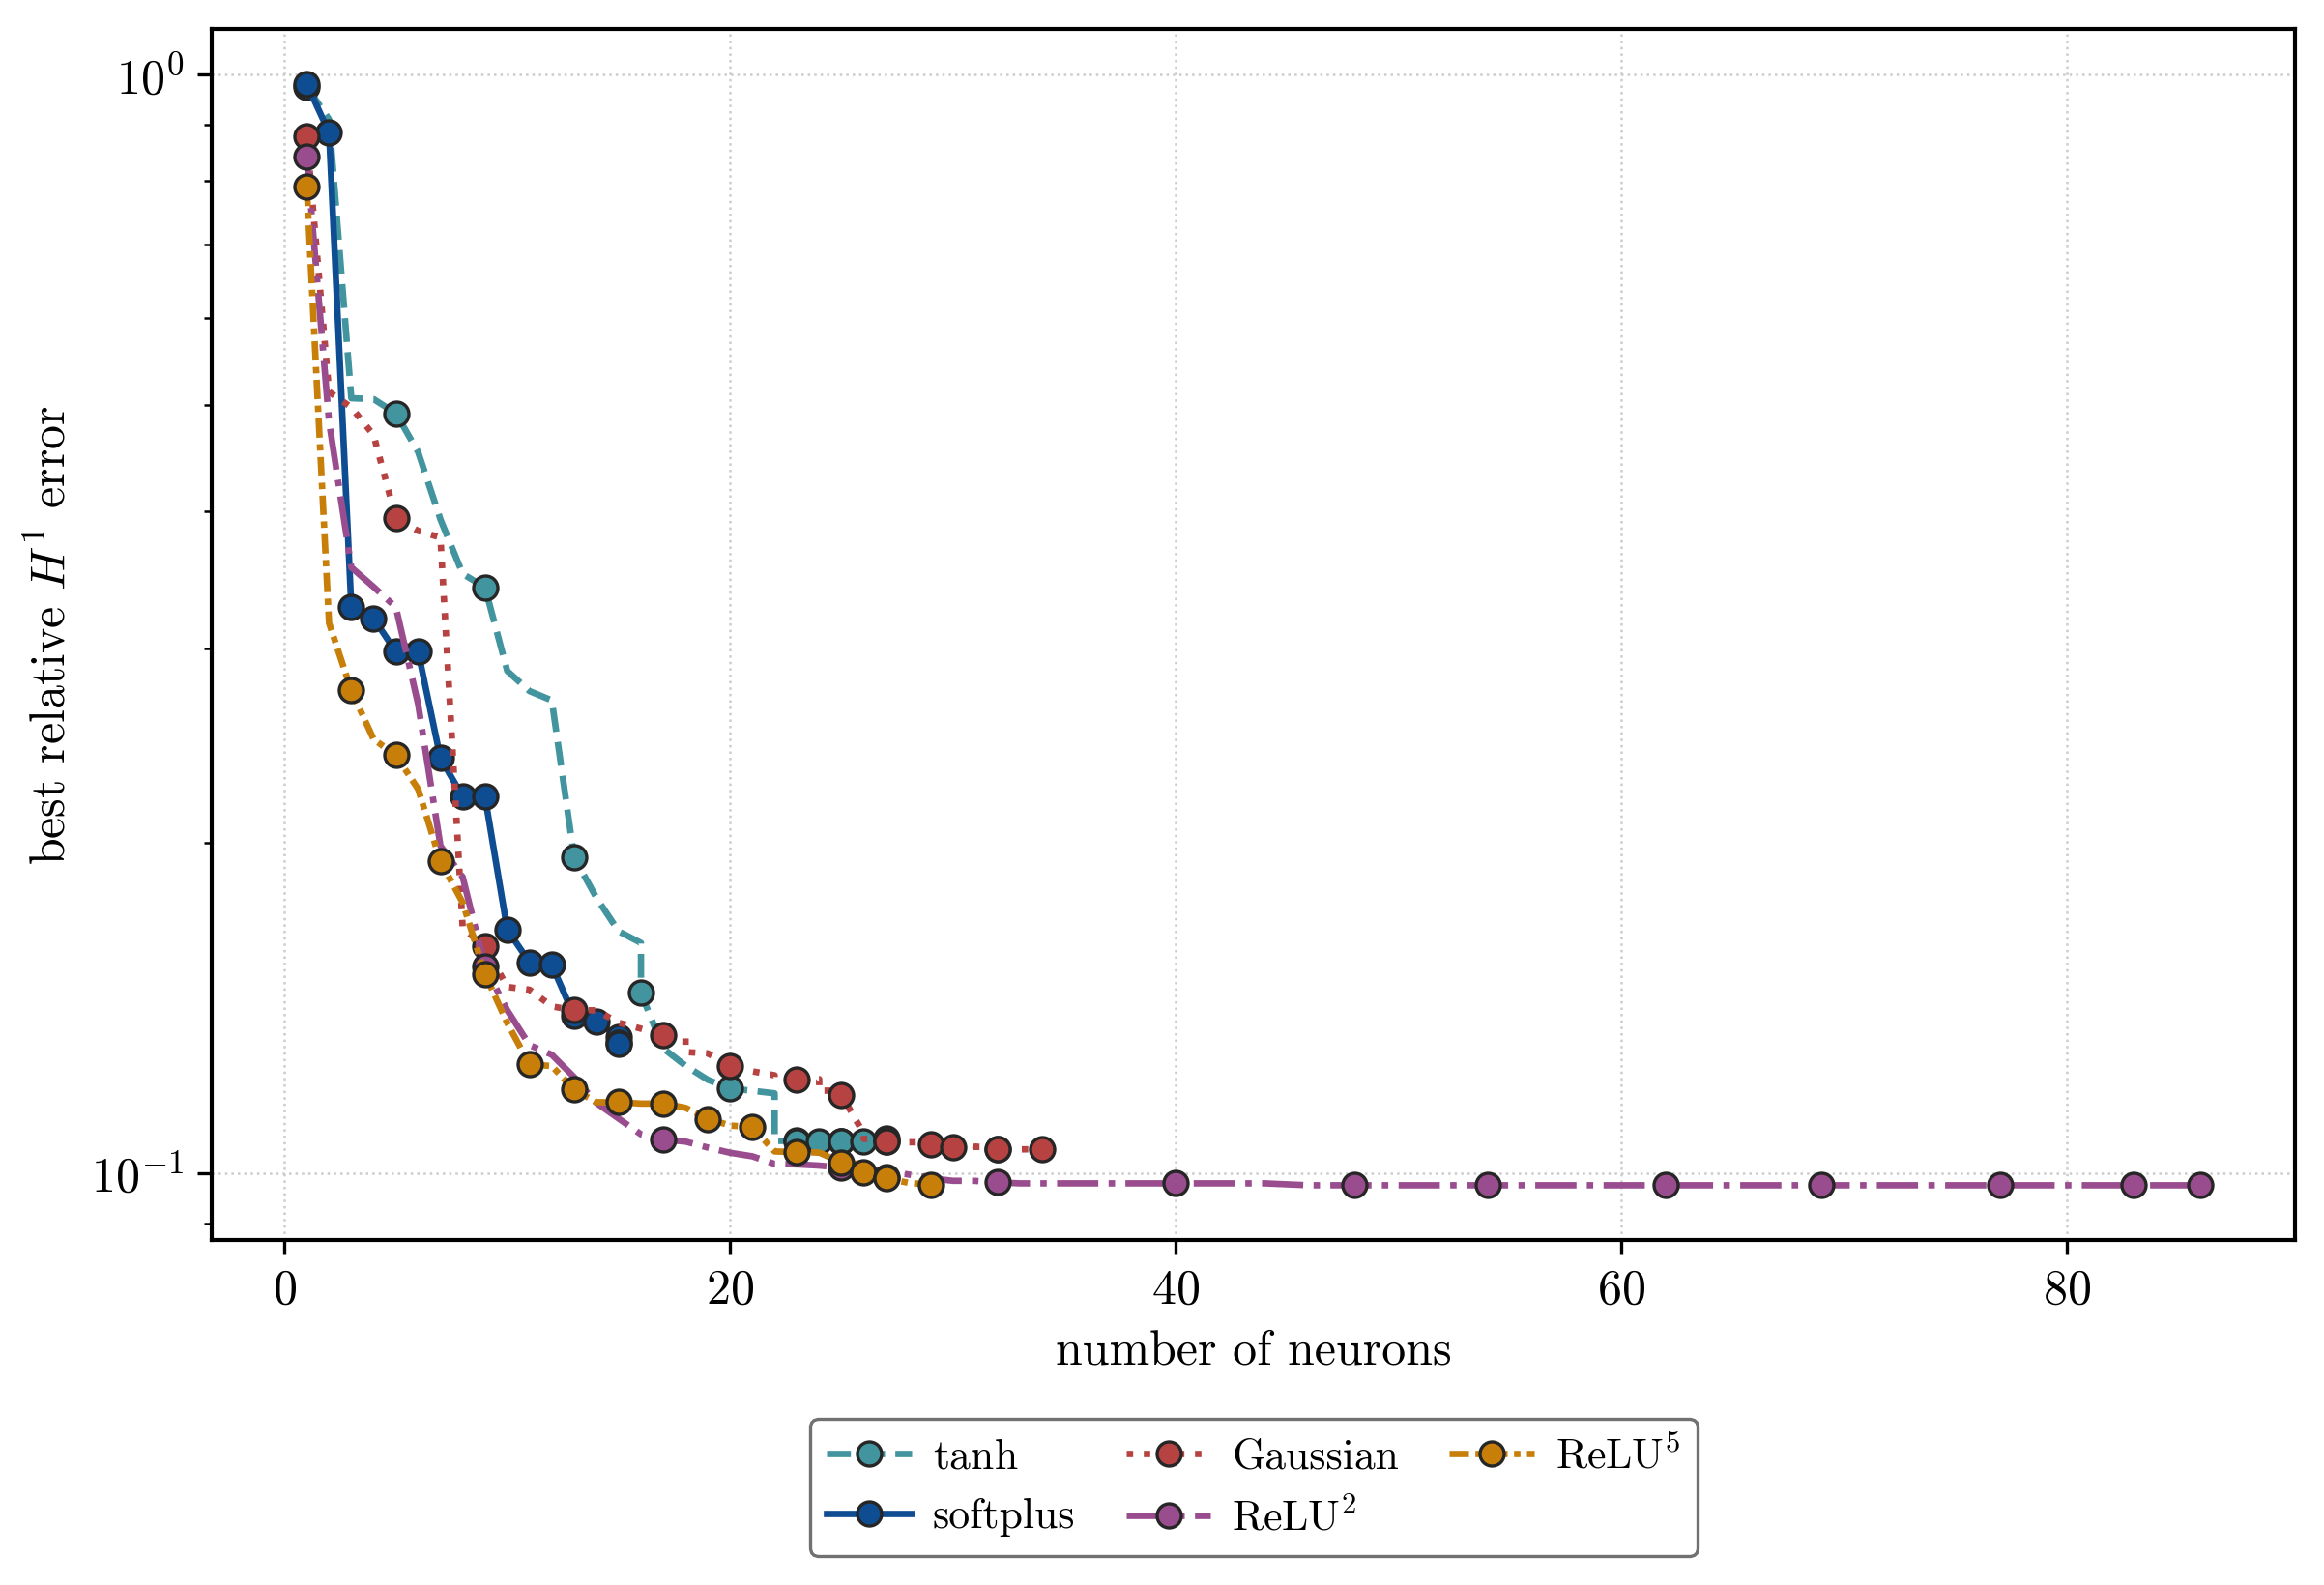
\includegraphics[width=0.8\textwidth]{../experiments/01_vdp/paper_log_penalty/figures/frontier.png}
\caption{Running best relative $H^1$ validation error against support size.
Nonhomogeneous profiles use the parameter values stated in
Table~\ref{tab:alg1_gradient}; homogeneous profiles use $\alpha\psi_k$ at
$\alpha=10^{-6}$ for both $k=2$ and $k=3$.}
\label{fig:summary_frontier}
\end{figure}

We synthesize feedback laws from $y_0 = (2, 1)$ and roll them out over the horizon $T = 12$ with fixed-step RK4, zero-order-hold controls clipped to $|u| \le 50$ as a numerical guard.
The reference law interpolates the time-zero costate component of the dataset
with a $C^1$ Clough--Tocher interpolant and applies it as a stationary
feedback. The finite-horizon optimal feedback is time-dependent and the
rollout horizon exceeds the data horizon $T=3$. Therefore its rollout cost
$6.48$ is not $V(0,y_0)$, and the comparison is not a test of finite-horizon
optimality.
Figure~\ref{fig:summary_feedback} shows $\|y(t)\|$ and $|u(t)|$ for softplus, the Gaussian, and $\reluk$ ($k = 3$), beside this reference. All three drive the state to the origin and track the reference control, at essentially its closed-loop cost ($6.48$, $6.50$, $6.49$ vs.\ $6.48$).
\begin{figure}[htbp]
\centering
\captionsetup[subfigure]{justification=centering}
\begin{subfigure}[t]{0.48\textwidth}
\centering
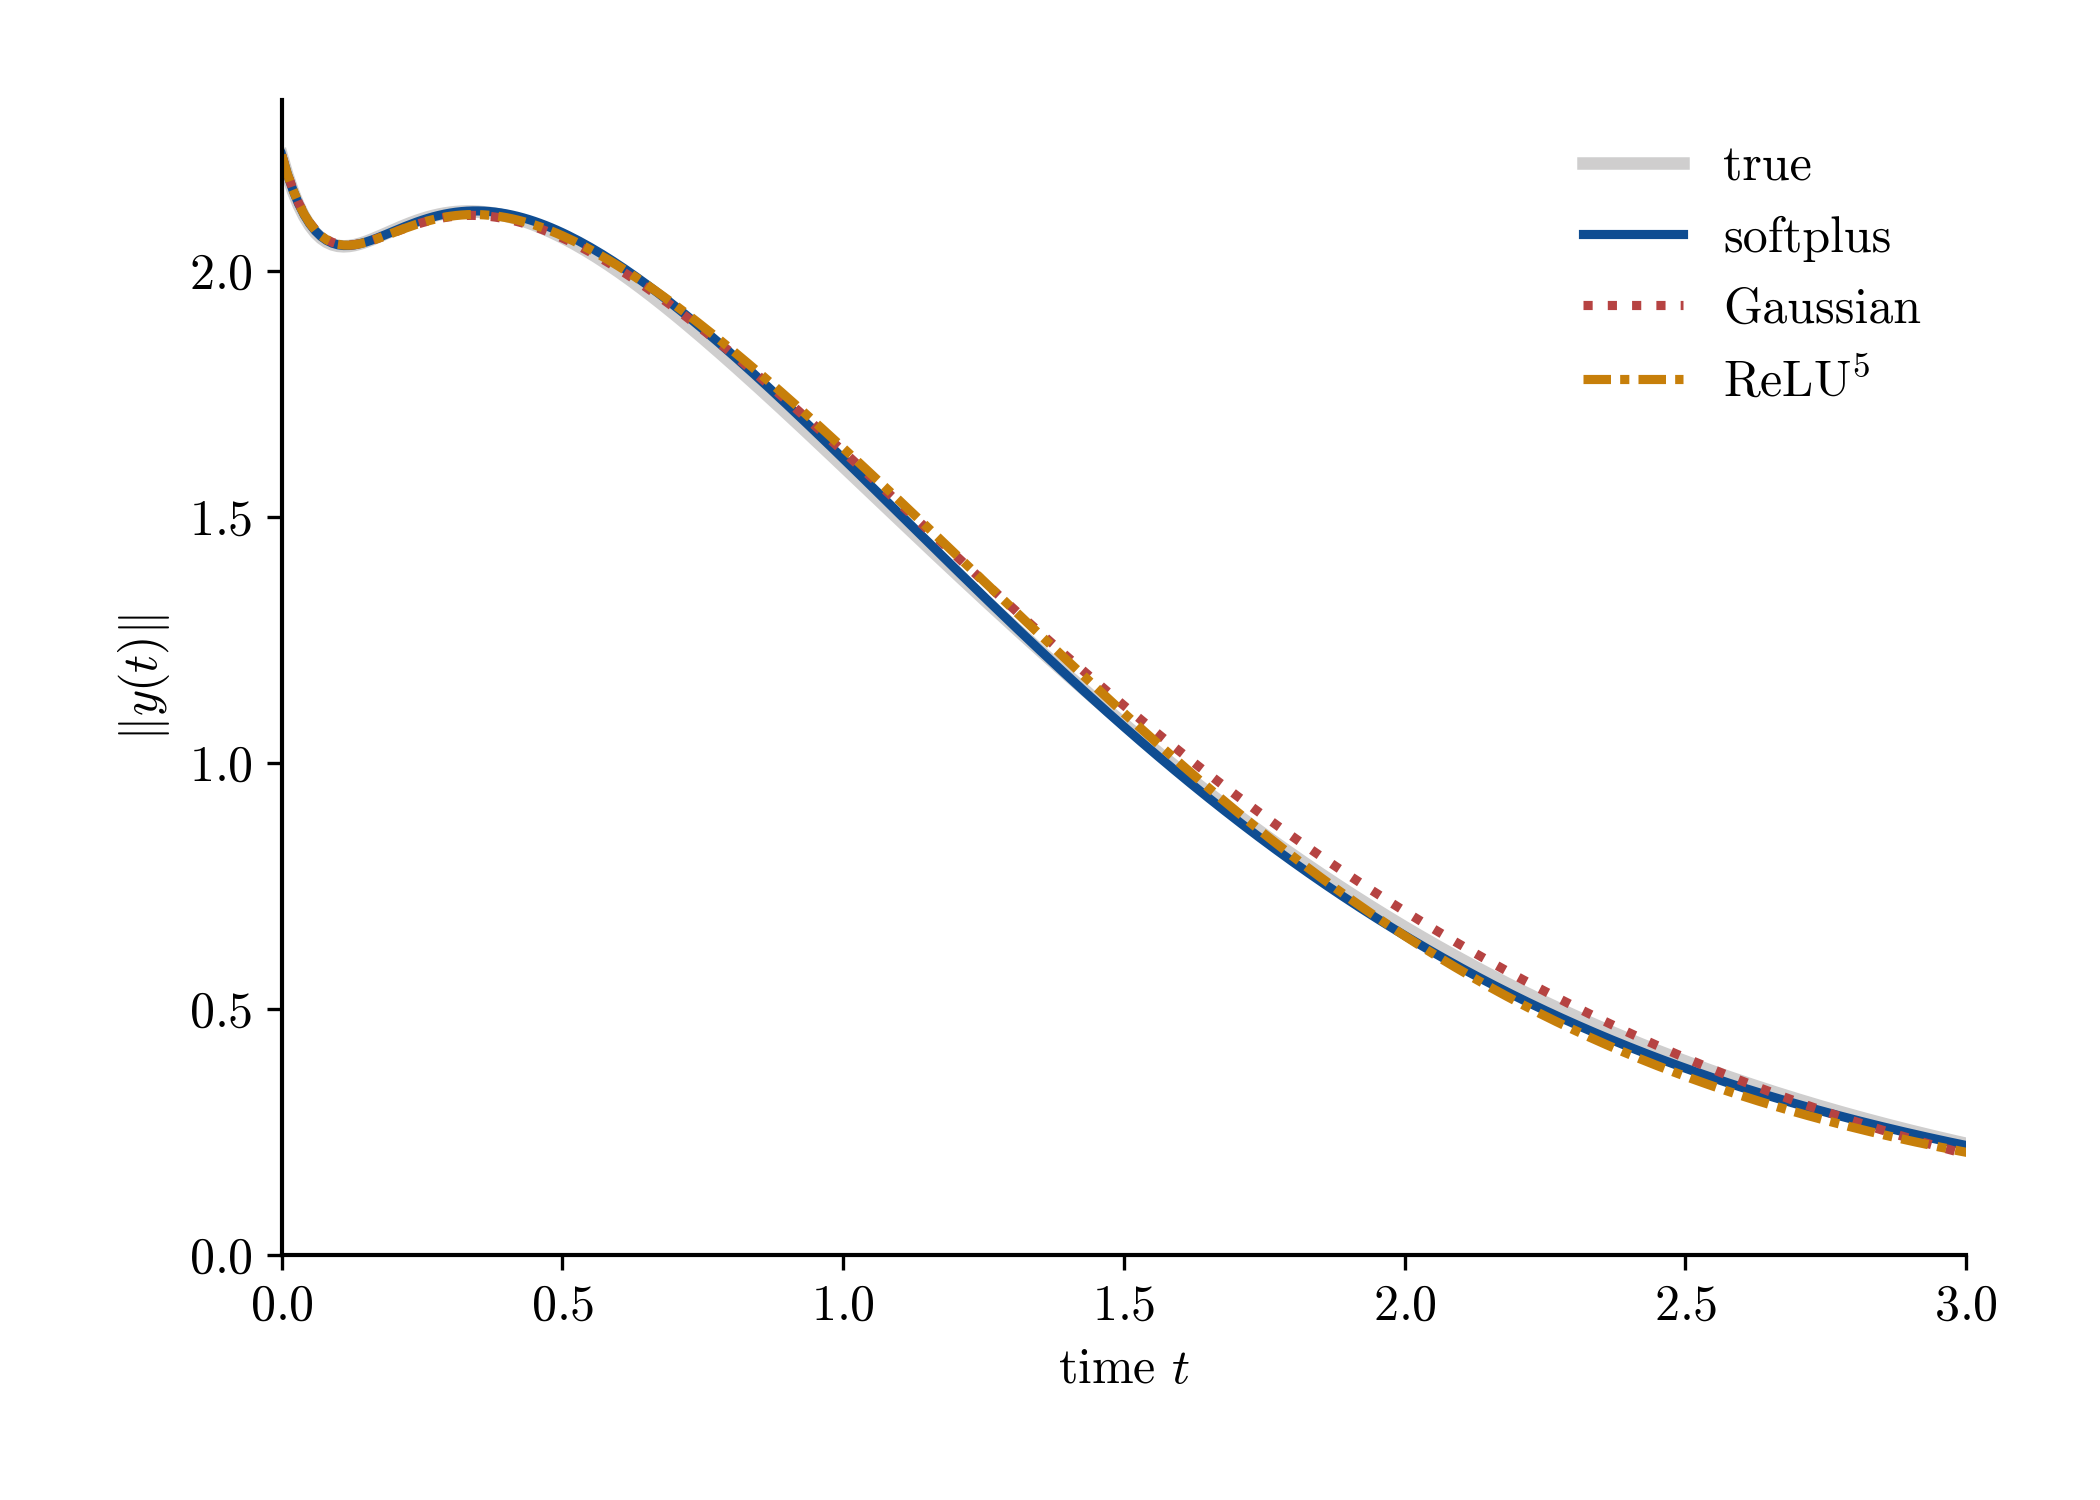
\includegraphics[width=\textwidth]{../experiments/01_vdp/paper_log_penalty/figures/feedback_state.png}
\caption{State norm $\|y(t)\|$.}
\label{fig:summary_feedback_state}
\end{subfigure}
\hfill
\begin{subfigure}[t]{0.48\textwidth}
\centering
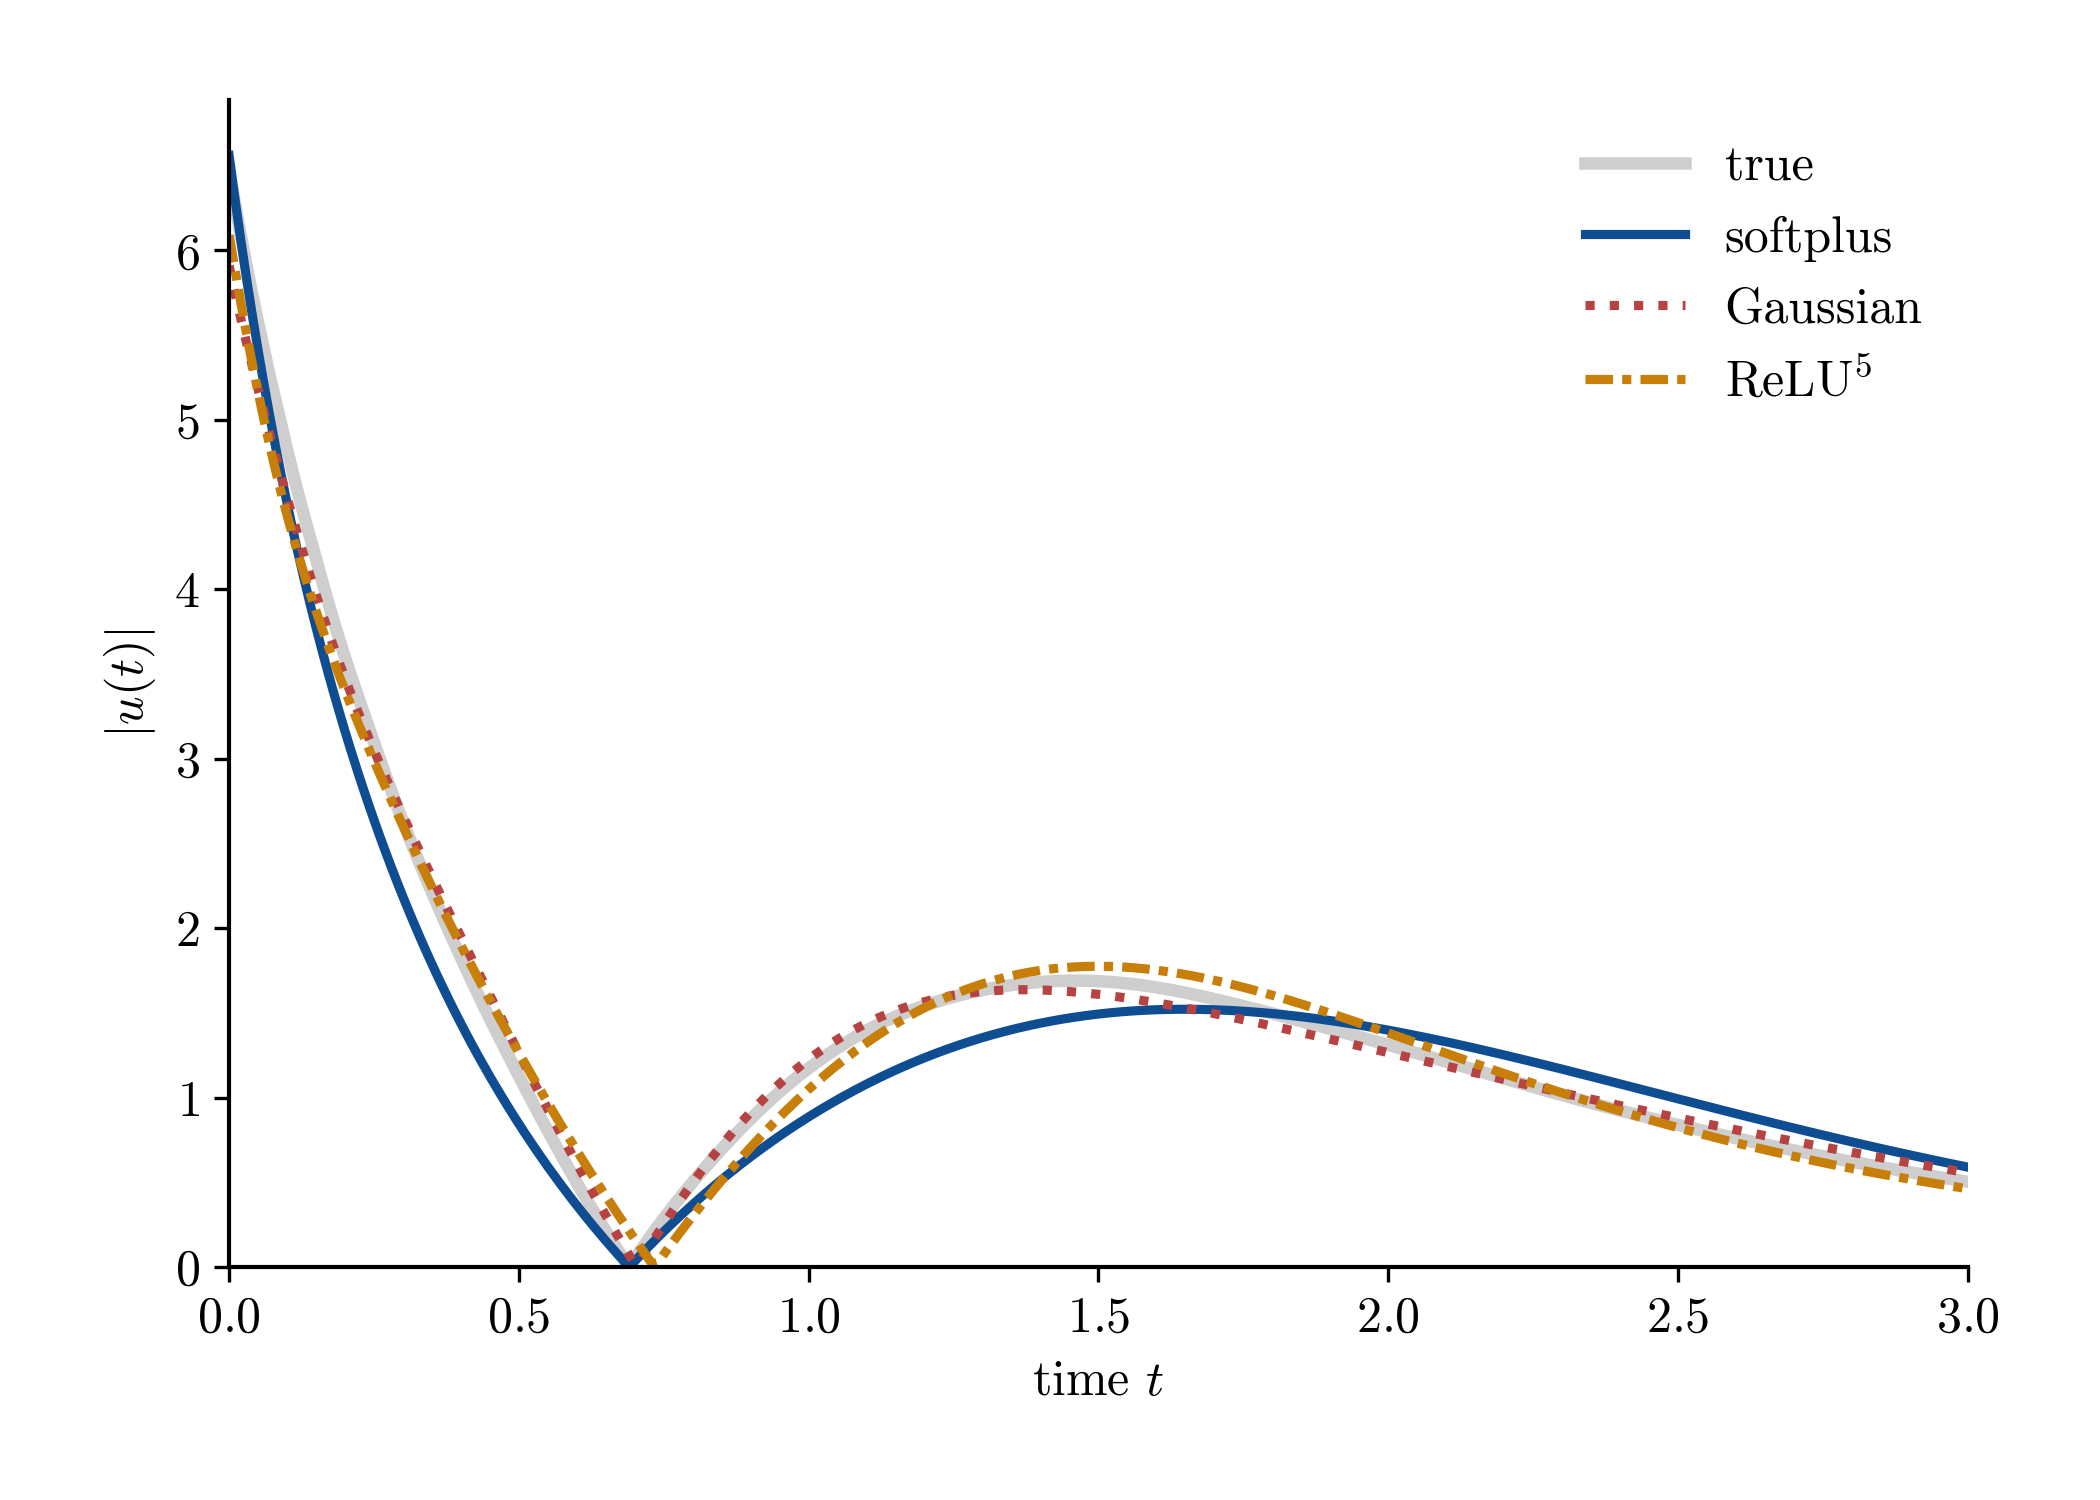
\includegraphics[width=\textwidth]{../experiments/01_vdp/paper_log_penalty/figures/feedback_control.png}
\caption{Control $|u(t)|$.}
\label{fig:summary_feedback_control}
\end{subfigure}
\caption{Evolution of the state and control from $y_0=(2,1)$ under the
feedback synthesized from each fitted value function and under the stationary
reference law obtained from the time-zero costates.}
\label{fig:summary_feedback}
\end{figure}

Figure~\ref{fig:summary_weights_raw} shows the inner parameters for the
Gaussian, softplus, and $\reluk$ ($k = 3$).
The two algorithms produce structurally different representations: Algorithm~2 constrains its atoms to the unit sphere $\mathbb{S}^2$, while Algorithm~1 leaves them free --- the Gaussian atoms in particular span a wide range of norms.
\begin{figure}[htbp]
\centering
\captionsetup[subfigure]{justification=centering}
\begin{subfigure}[t]{0.32\textwidth}
\centering
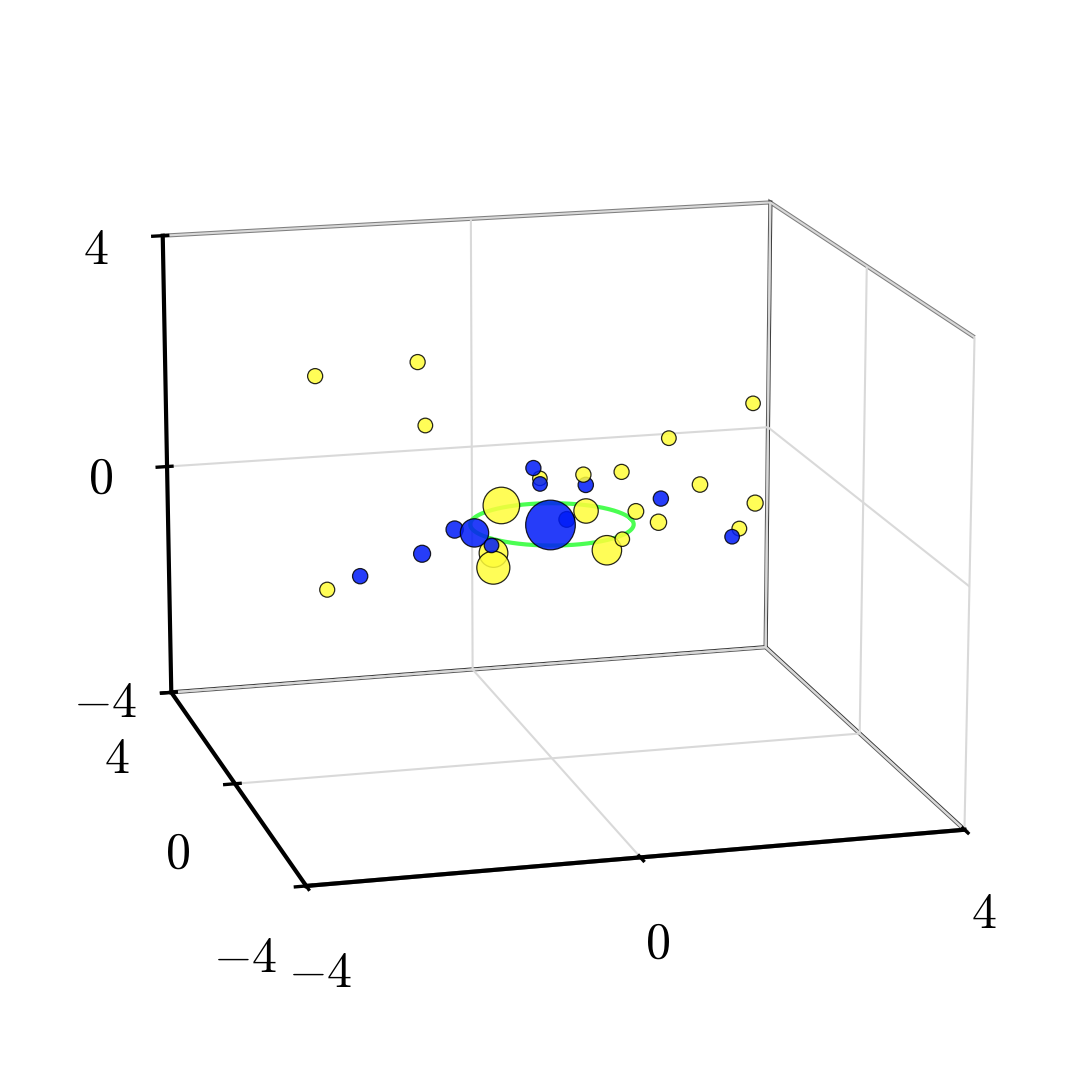
\includegraphics[width=\textwidth]{../experiments/01_vdp/paper_log_penalty/figures/weights_raw3d_gaussian.png}
\caption{Gaussian.}
\end{subfigure}
\hfill
\begin{subfigure}[t]{0.32\textwidth}
\centering
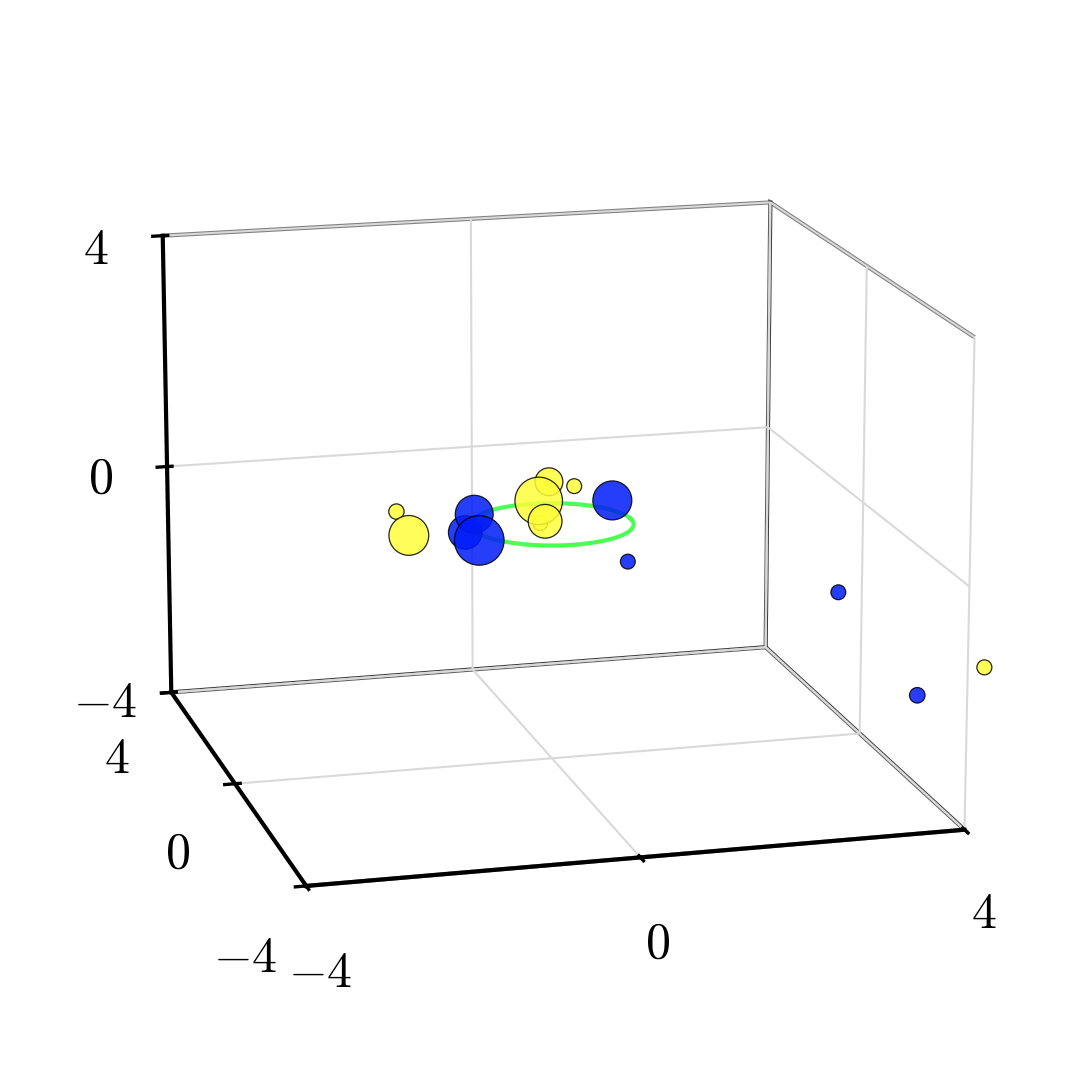
\includegraphics[width=\textwidth]{../experiments/01_vdp/paper_log_penalty/figures/weights_raw3d_softplus.png}
\caption{softplus.}
\end{subfigure}
\hfill
\begin{subfigure}[t]{0.32\textwidth}
\centering
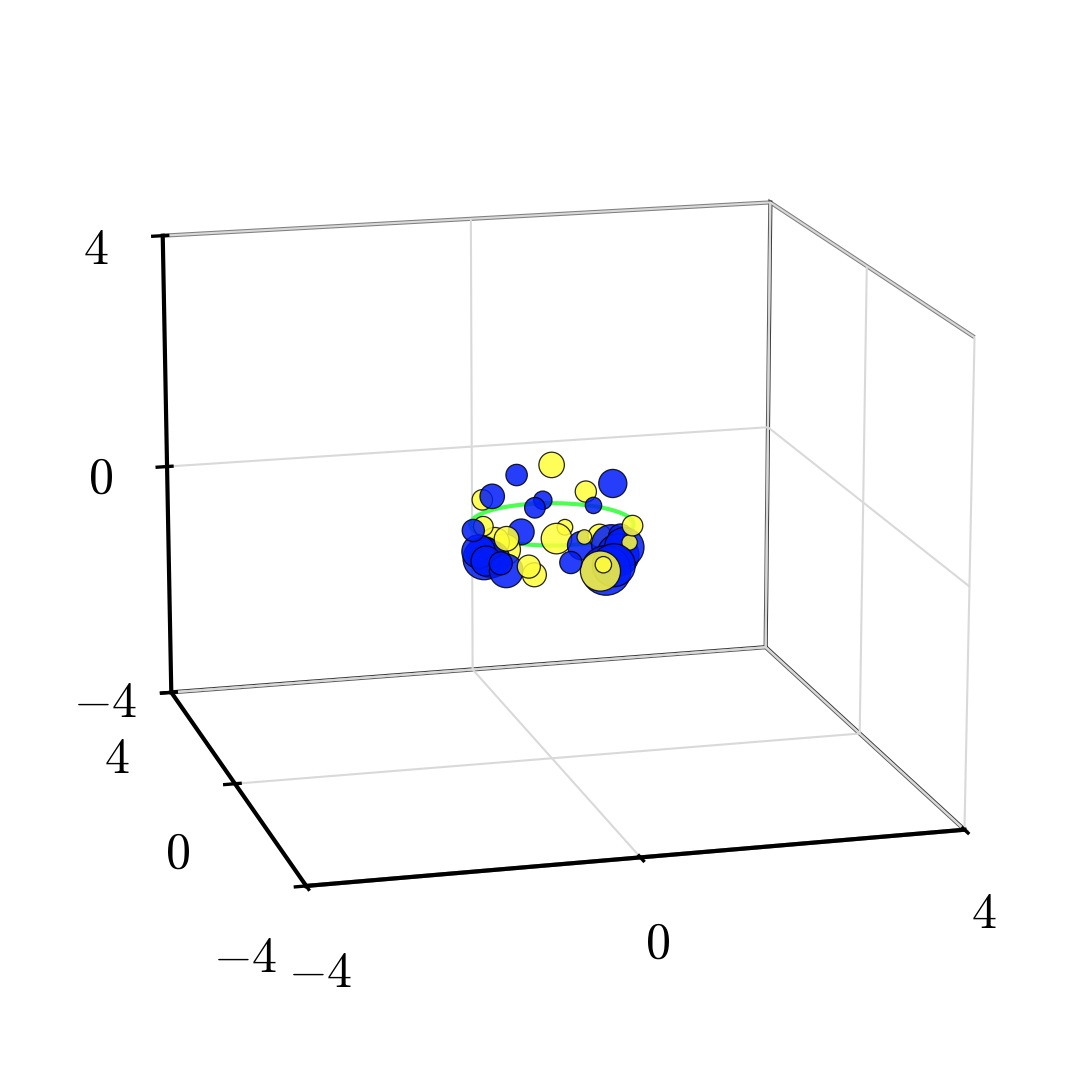
\includegraphics[width=\textwidth]{../experiments/01_vdp/paper_log_penalty/figures/weights_raw3d_relu3.png}
\caption{$\mathrm{ReLU}^3 + \alpha\,\psi_3$.}
\end{subfigure}
\caption{Inner parameters $(a_1,a_2,b)$, with the unit circle in the plane
$b=0$ shown in light green. The two nonhomogeneous fits use
$\alpha=10^{-4}$, $\gamma=10$, $p=2.01$; dot color gives the
sign and dot size the magnitude of the outer weight.}
\label{fig:summary_weights_raw}
\end{figure}



\subsection{Pendulum Swing-Up}
The question in this example is how a sparse gradient-trained network
approximates a continuous value function whose gradient jumps across a
switching set. A finite network with a continuously differentiable activation
has a continuous gradient and therefore cannot reproduce the jump exactly.

The example we consider follows from \cite{han2024nonsmooth}.
We write the state as
\begin{equation*}
	x = (x_1,x_2)^\top = (\theta,\dot{\theta})^\top,
\end{equation*}
the pendulum angle and angular velocity. (The letter $\omega$ remains reserved
for the network parameters.)
We consider the optimal control problem
\begin{equation*}
\min_{u \in L^2(0,\infty;\mathbb{R})}\mathcal C(u;0,x)
=\int_0^\infty \big(
\sin^2\theta(t)+(\cos\theta(t)-1)^2+\dot{\theta}^2(t)+\eta u^2(t)
\big)\,dt
\end{equation*}
subject to
\begin{equation*}
\begin{cases}
	m\ell^2\,\ddot{\theta} = -b\dot{\theta} + mg\ell\sin\theta + u,\\
	(\theta(0),\dot{\theta}(0))=(x_1,x_2).
\end{cases}
\end{equation*}
The target equilibria are
$x_{U,j}:=(2j\pi,0)$, $j\in\mathbb Z$; for a selected target we write
$x_U=x_{U,j}$.

In this setting the state dimension is $d=2$ and the control is scalar.
The physical and cost parameters are $m = \ell = 1$, $b = 0.1$, $g = 9.8$,
and $\eta = 1$.
To initialize the backward integration, we use the local linear-quadratic regulator (LQR) approximation near $x_U$.
Let $\widetilde x=x-x_U$ be the local coordinate around the upright equilibrium.
Linearizing the dynamics at $(x_U,0)$ gives
\begin{equation*}
	\dot{\widetilde x}=A\widetilde x+Bu,\quad
	A=\begin{pmatrix}0&1\\ \frac{g}{\ell}&-\frac{b}{m\ell^2}\end{pmatrix},
	\quad
	B=\begin{pmatrix}0\\ \frac{1}{m\ell^2}\end{pmatrix}.
\end{equation*}
The running cost is locally approximated by
\begin{equation*}
	|\widetilde x|^2+\eta u^2.
\end{equation*}
The local infinite-horizon LQR value function is
\begin{equation*}
	V^\infty(\widetilde x)=\widetilde x^\top P\widetilde x,
\end{equation*}
where $P$ is the positive definite solution of the algebraic Riccati equation
\begin{equation*}
	A^\top P+PA-\frac{1}{\eta}PBB^\top P+I_2=0.
\end{equation*}
The superscript $\infty$ refers to the infinite-horizon LQR problem.
For $\varepsilon>0$, we define the local LQR sublevel set and boundary by
\begin{equation*}
	\mathcal E_\varepsilon
	=\{\widetilde x:V^\infty(\widetilde x)\leq \varepsilon\},
	\qquad
	\partial\mathcal E_\varepsilon
	=\{\widetilde x:V^\infty(\widetilde x)=\varepsilon\}.
\end{equation*}
The corresponding state-costate system becomes
\begin{equation}
\label{TPBVP_pendulum}
\left\{
\begin{aligned}
	& m\ell^2\,\ddot{\theta}^* = -b\dot{\theta}^* + mg\ell\sin\theta^* + u^*,\\
	& -\dot{p}_1^* = 2\sin\theta^* + \frac{g}{\ell}\cos\theta^*\,p_2^*,\\
	& -\dot{p}_2^* = 2\dot{\theta}^* + p_1^* - \frac{b}{m\ell^2}p_2^*,\\
	& x^*(0)=x,\quad x^*(T_x)-x_U\in\partial\mathcal E_\varepsilon,
	\quad p^*(T_x)=\nabla V^\infty(x^*(T_x)-x_U).
\end{aligned}
\right.
\end{equation}
In the experiment we use $\varepsilon=2\times 10^{-4}$, and on
$\partial\mathcal E_\varepsilon$ the terminal costate is
\begin{equation*}
	p^*(T_x)=\nabla V^\infty(\widetilde x^*(T_x))
	=2P\widetilde x^*(T_x).
\end{equation*}
For the data generation, we integrate $2000$ PMP paths backward from the local
LQR boundary $\partial\mathcal E_\varepsilon$. Along each path, the accumulated
running cost plus the boundary value $\varepsilon$ gives $V(x)$, and the
costate gives the label $g=p$. At differentiability points, $g=\nabla V(x)$.
The backward integration stops when the
accumulated value reaches $100$; the training samples are restricted to
values below $50$.
This yields the dataset
\begin{equation*}
\{x^m,V(x^m),g^m\}_{m=1}^M.
\end{equation*}

The construction provides samples on both sides of the gradient
discontinuity. For $j\in\mathbb Z$, let $V_{2j\pi}(x)$ be the fixed-target
value obtained by minimizing over paths that reach the local LQR
neighbourhood of $(2j\pi,0)$. The stationary value is
\begin{equation*}
	V(x)=\min_{j\in\mathbb Z}V_{2j\pi}(x).
\end{equation*}
In the region where the targets $(0,0)$ and $(2\pi,0)$ are minimizing, this
reduces to $V(x)=\min\{V_0(x),V_{2\pi}(x)\}$. Define the representative
switching set between these adjacent targets by
\begin{equation*}
	S_{0,2\pi}:=\{x\in\mathbb R^2:V_0(x)=V_{2\pi}(x)=V(x)\}.
\end{equation*}
On the numerical domain $D=[-8,8]^2$, the periodic switching set and its
closed $\delta$-neighbourhood are
\begin{equation*}
	S:=D\cap\bigcup_{j\in\mathbb Z}
	\bigl(S_{0,2\pi}+(2j\pi,0)\bigr),
	\qquad
	S_\delta:=\{x\in D:\operatorname{dist}(x,S)\le\delta\},
	\qquad \delta>0.
\end{equation*}
The regional errors below use $\delta=0.3$.
At points of $S$, two adjacent fixed-target values agree while their gradients
may differ; the sampled PMP costates provide the corresponding one-sided
gradients, without asserting a classical gradient on $S$.

To reconstruct $S_{0,2\pi}$, fix a value level $\ell$ and interpolate one
state with value $\ell$ on each raw PMP path. Ordering these states by their
terminal-boundary angle gives a polygonal approximation of
$\{x:V_0(x)=\ell\}$. By periodicity, translating this contour by
$(2\pi,0)$ gives the corresponding approximation of
$\{x:V_{2\pi}(x)=\ell\}$. Every intersection of the two contours therefore
satisfies $V_0(x)=V_{2\pi}(x)=\ell$. Repeating the construction over the
sampled value levels and tracking the four intersections nearest $(\pi,0)$
produces the four arms of $S_{0,2\pi}$; their $2\pi$-translates give $S$ in
$D$.

After reconstructing $S$, we augment the dataset with samples from both value
branches. By periodicity, translating a raw PMP path by $\pm2\pi$ in $\theta$
produces a path associated with an adjacent upright. Not every translated
state belongs to the optimal branch, so we keep only states within distance
$0.5$ of $S$ for which a local first-order comparison identifies the branch as
strictly cheaper than its competitor.
Together with the $3{,}000$ original PMP samples, the final dataset contains
$3{,}900$ samples and costate labels from both sides of the gradient
discontinuity. Figure~\ref{fig:pendulum_data} shows the resulting dataset.
\begin{figure}[htbp]
\centering
\captionsetup[subfigure]{justification=centering}
\begin{subfigure}[b]{0.32\textwidth}
\centering

\includegraphics[width=\textwidth]{plot/pendulum_value_scatter.png}
\caption{value samples $\{x^m, V(x^m)\}$.}
\label{fig:pendulum_data_scatter}
\end{subfigure}
\hfill
\begin{subfigure}[b]{0.32\textwidth}
\centering
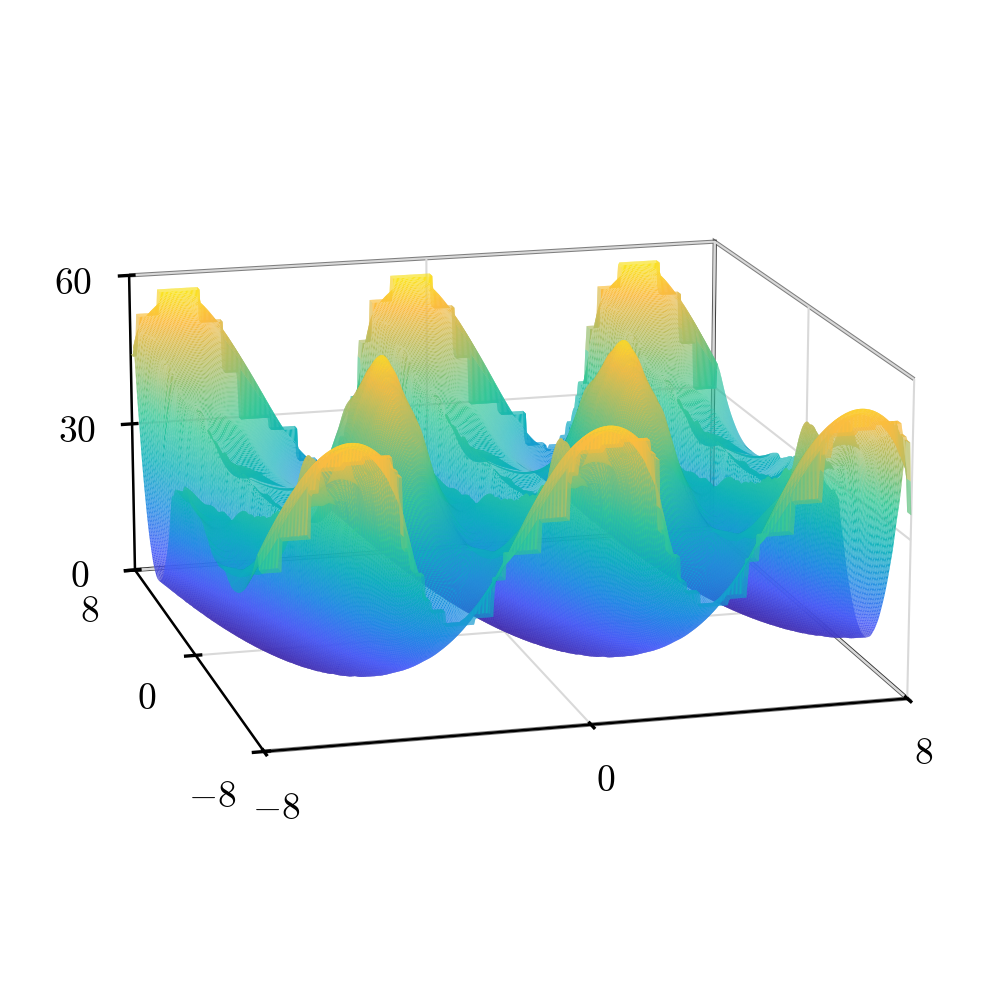
\includegraphics[width=\textwidth]{plot/pendulum_value_surface.png}
\caption{value surface $V(x)$.}
\label{fig:pendulum_data_surface}
\end{subfigure}
\hfill
\begin{subfigure}[b]{0.32\textwidth}
\centering

\includegraphics[width=\textwidth]{plot/pendulum_regions.png}
\caption{regions associated with the periodic targets.}
\label{fig:pendulum_data_regions}
\end{subfigure}
\caption{Optimal value function $V(x)$ over the $(\theta, \dot\theta)$ plane,
$2\pi$-periodic in $\theta$. (a) The raw $(x, V)$ samples produced by the PMP
generator. (b) The reconstructed value surface. (c) Regions where $V_0$ or
another periodic fixed-target value is minimal; their boundaries form $S$,
across which $\nabla V$ may be discontinuous.}
\label{fig:pendulum_data}
\end{figure}

\subsubsection{Approximation near the switching set}
Figure~\ref{fig:rs_surfaces} shows the fitted surfaces on the same physical
window and value range as the value function in
Figure~\ref{fig:pendulum_data_surface}. The cross-section below compares the
approximations near $S$.

\begin{figure}[htbp]
\centering
\captionsetup[subfigure]{justification=centering}
\begin{subfigure}[b]{0.19\textwidth}
\centering
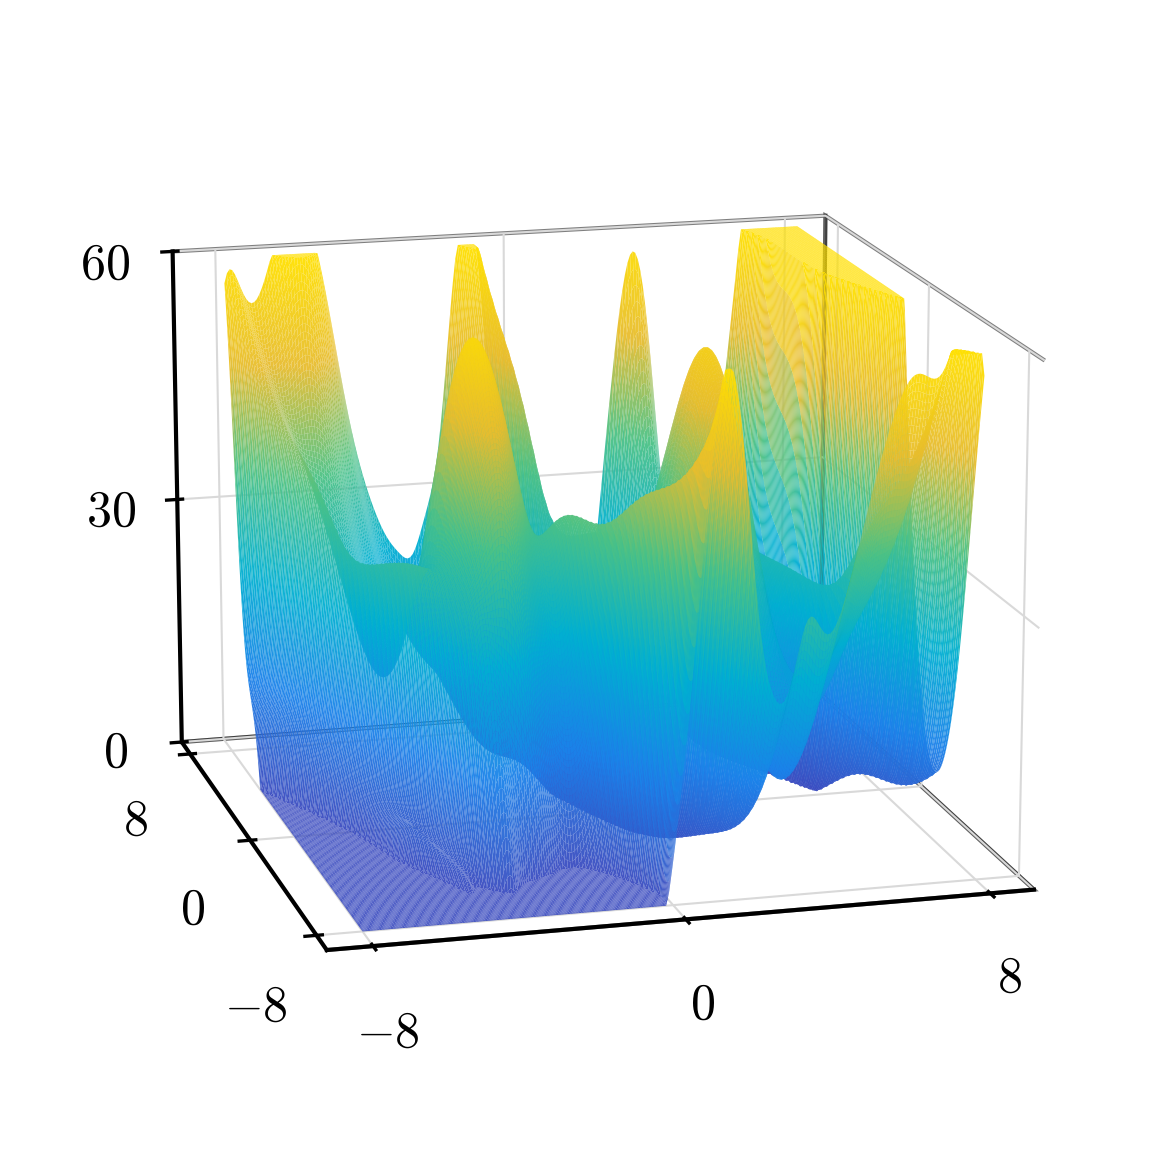
\includegraphics[width=\textwidth]{../experiments/02_pendulum/paper_log_penalty/figures/surface_gaussian.png}
\caption{Gaussian}
\label{fig:rs_surface_gaussian}
\end{subfigure}
\hfill
\begin{subfigure}[b]{0.19\textwidth}
\centering
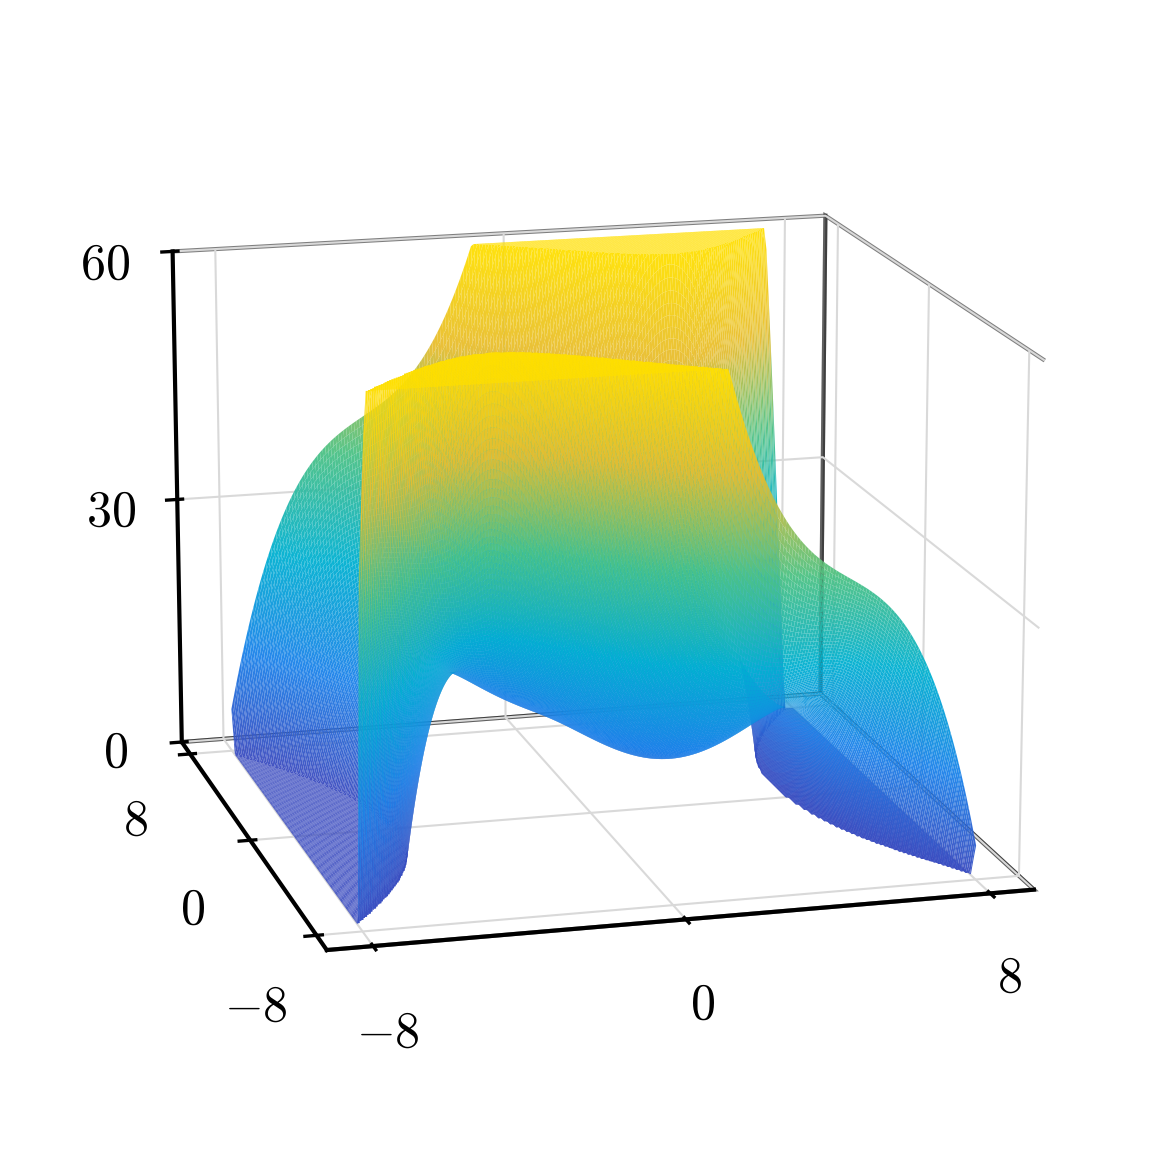
\includegraphics[width=\textwidth]{../experiments/02_pendulum/paper_log_penalty/figures/surface_softplus.png}
\caption{softplus}
\label{fig:rs_surface_softplus}
\end{subfigure}
\hfill
\begin{subfigure}[b]{0.19\textwidth}
\centering
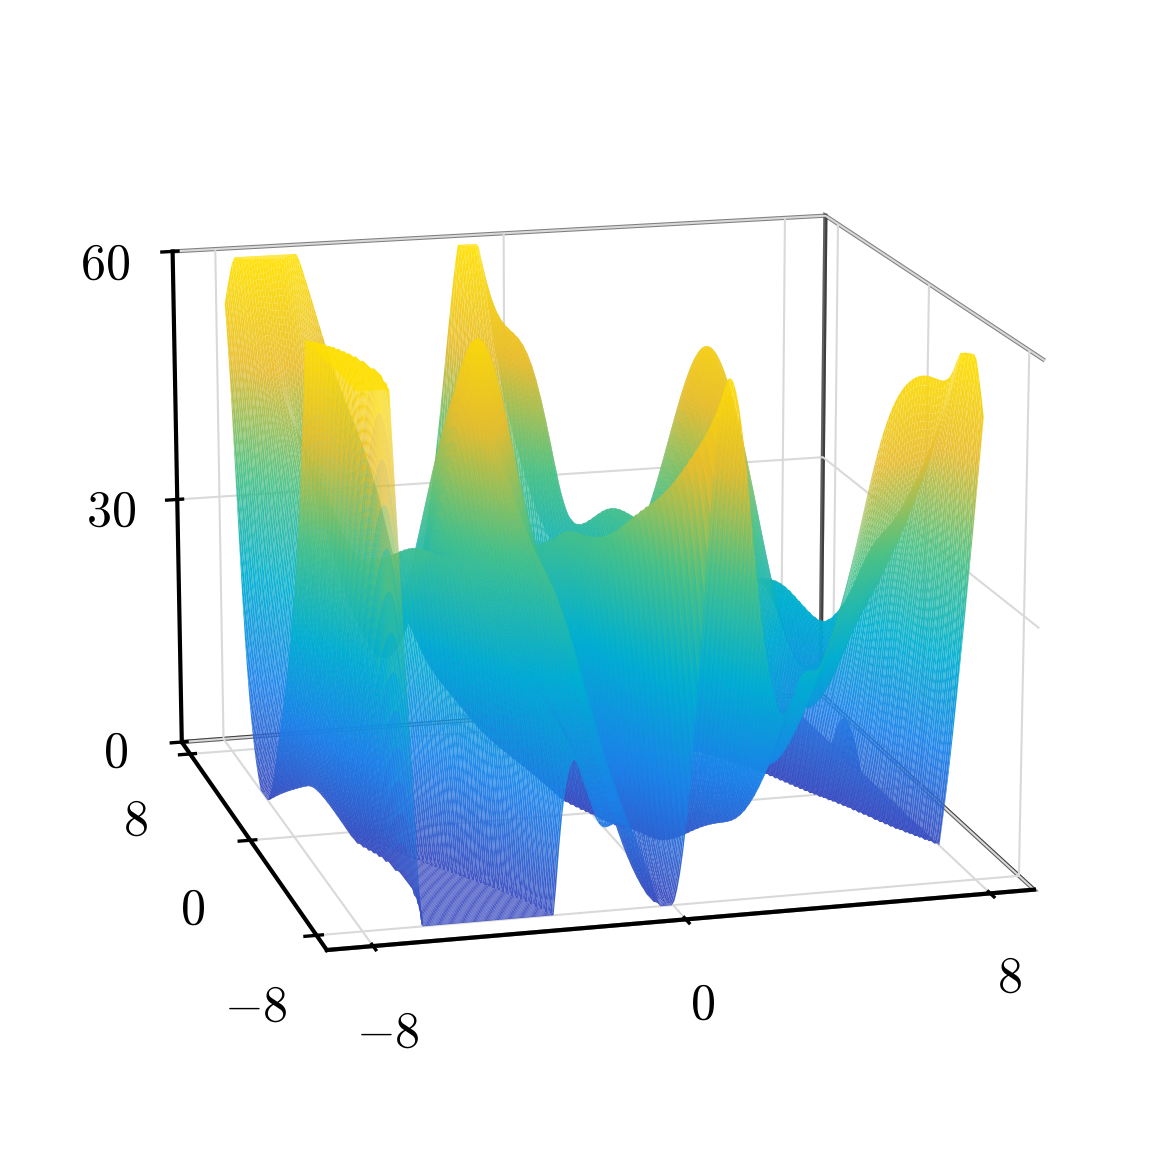
\includegraphics[width=\textwidth]{../experiments/02_pendulum/paper_log_penalty/figures/surface_tanh.png}
\caption{$\tanh$}
\label{fig:rs_surface_tanh}
\end{subfigure}
\hfill
\begin{subfigure}[b]{0.19\textwidth}
\centering
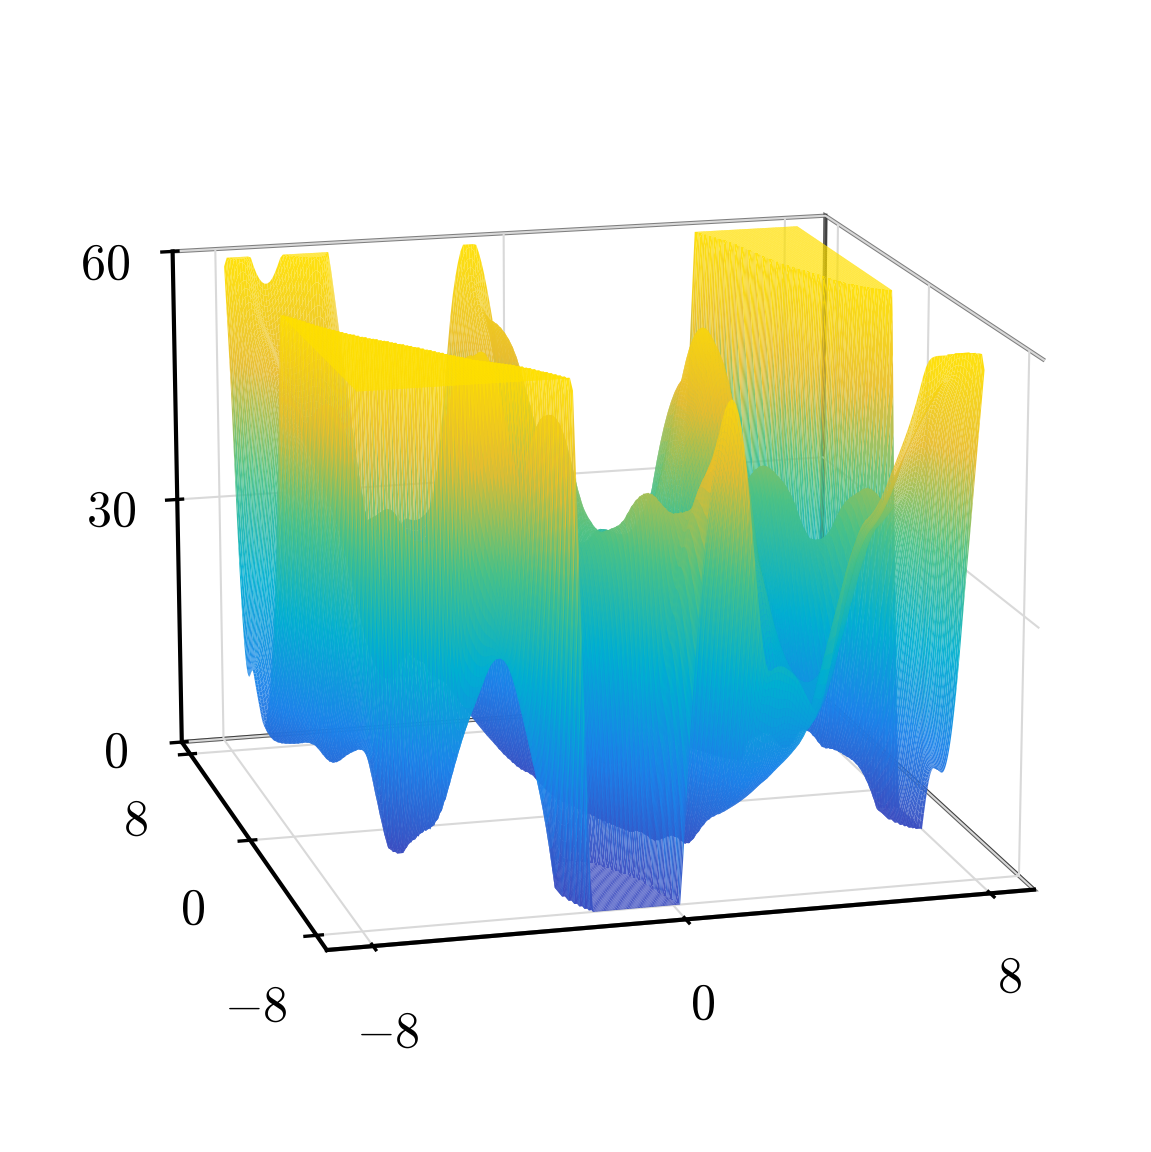
\includegraphics[width=\textwidth]{../experiments/02_pendulum/paper_log_penalty/figures/surface_relu2.png}
\caption{$\mathrm{ReLU}^{2}$}
\label{fig:rs_surface_relu2}
\end{subfigure}
\hfill
\begin{subfigure}[b]{0.19\textwidth}
\centering
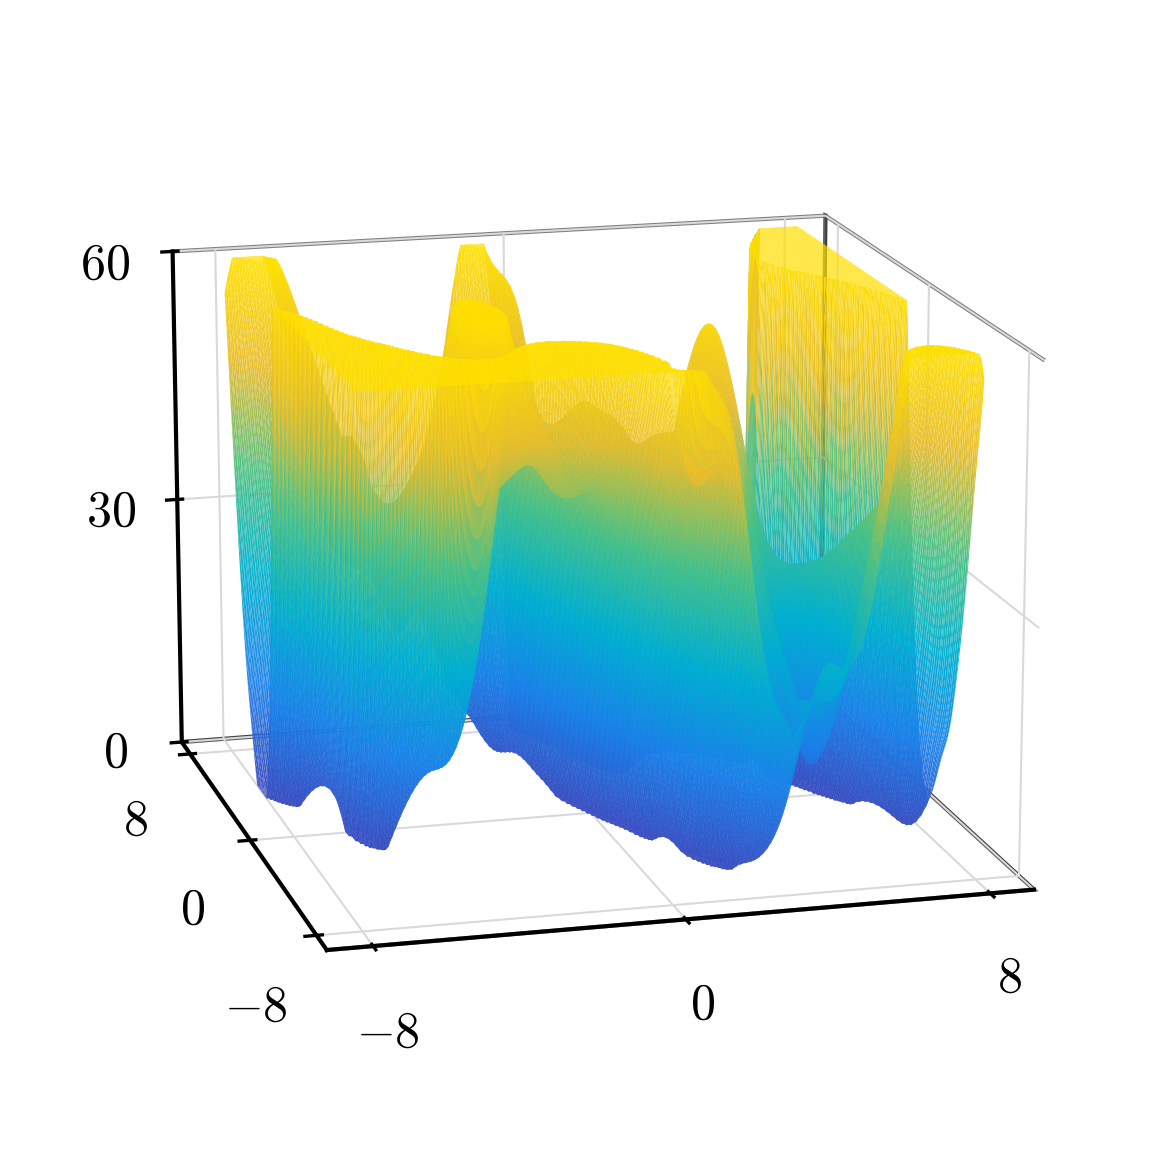
\includegraphics[width=\textwidth]{../experiments/02_pendulum/paper_log_penalty/figures/surface_relu3.png}
\caption{$\mathrm{ReLU}^{3}$}
\label{fig:rs_surface_relu3}
\end{subfigure}
\caption{Learned value surfaces $\widehat V(x)$ over the $(\theta,\dot\theta)$
window $[-8,8]^{2}$, displayed on the common range $\widehat V\in[0,60]$.
The $\reluk$ models are trained with the fractional-exponent penalty $\psi_k$,
and the nonhomogeneous models with \eqref{eq:empirical-log-objective} using the
parameter values reported in
Figure~\ref{fig:neuron_h1_frontier}\subref{fig:feedback_cost_a}.}
\label{fig:rs_surfaces}
\end{figure}

Let $x_S$ be the selected regular point of $S$ in the region,
and let $n$ be a unit normal to $S$ at $x_S$.
Figure~\ref{fig:rs_transect} shows the cross-section
$x(s)=x_S+sn$. Along this section,
$V=\min\{V_0,V_{2\pi}\}$. It has a kink at $s=0$, and the normal gradient
$n\cdot\nabla V$ jumps there.
No fitted model reproduces the magnitude of the jump: all undershoot the steep
gradient on the side $s<0$. Among the rectified powers,
$\mathrm{ReLU}^{2}$ has the smaller error on $S_{0.3}$ and develops the
sharpest change of slope near $s=0$; the smooth Gaussian, softplus, and $\tanh$
fits interpolate through the discontinuity.
The higher rectified powers remain smooth enough in their first derivative to
miss the jump.

\begin{figure}[htbp]
\centering
\captionsetup[subfigure]{justification=centering}
\begin{subfigure}[b]{0.48\textwidth}
\centering
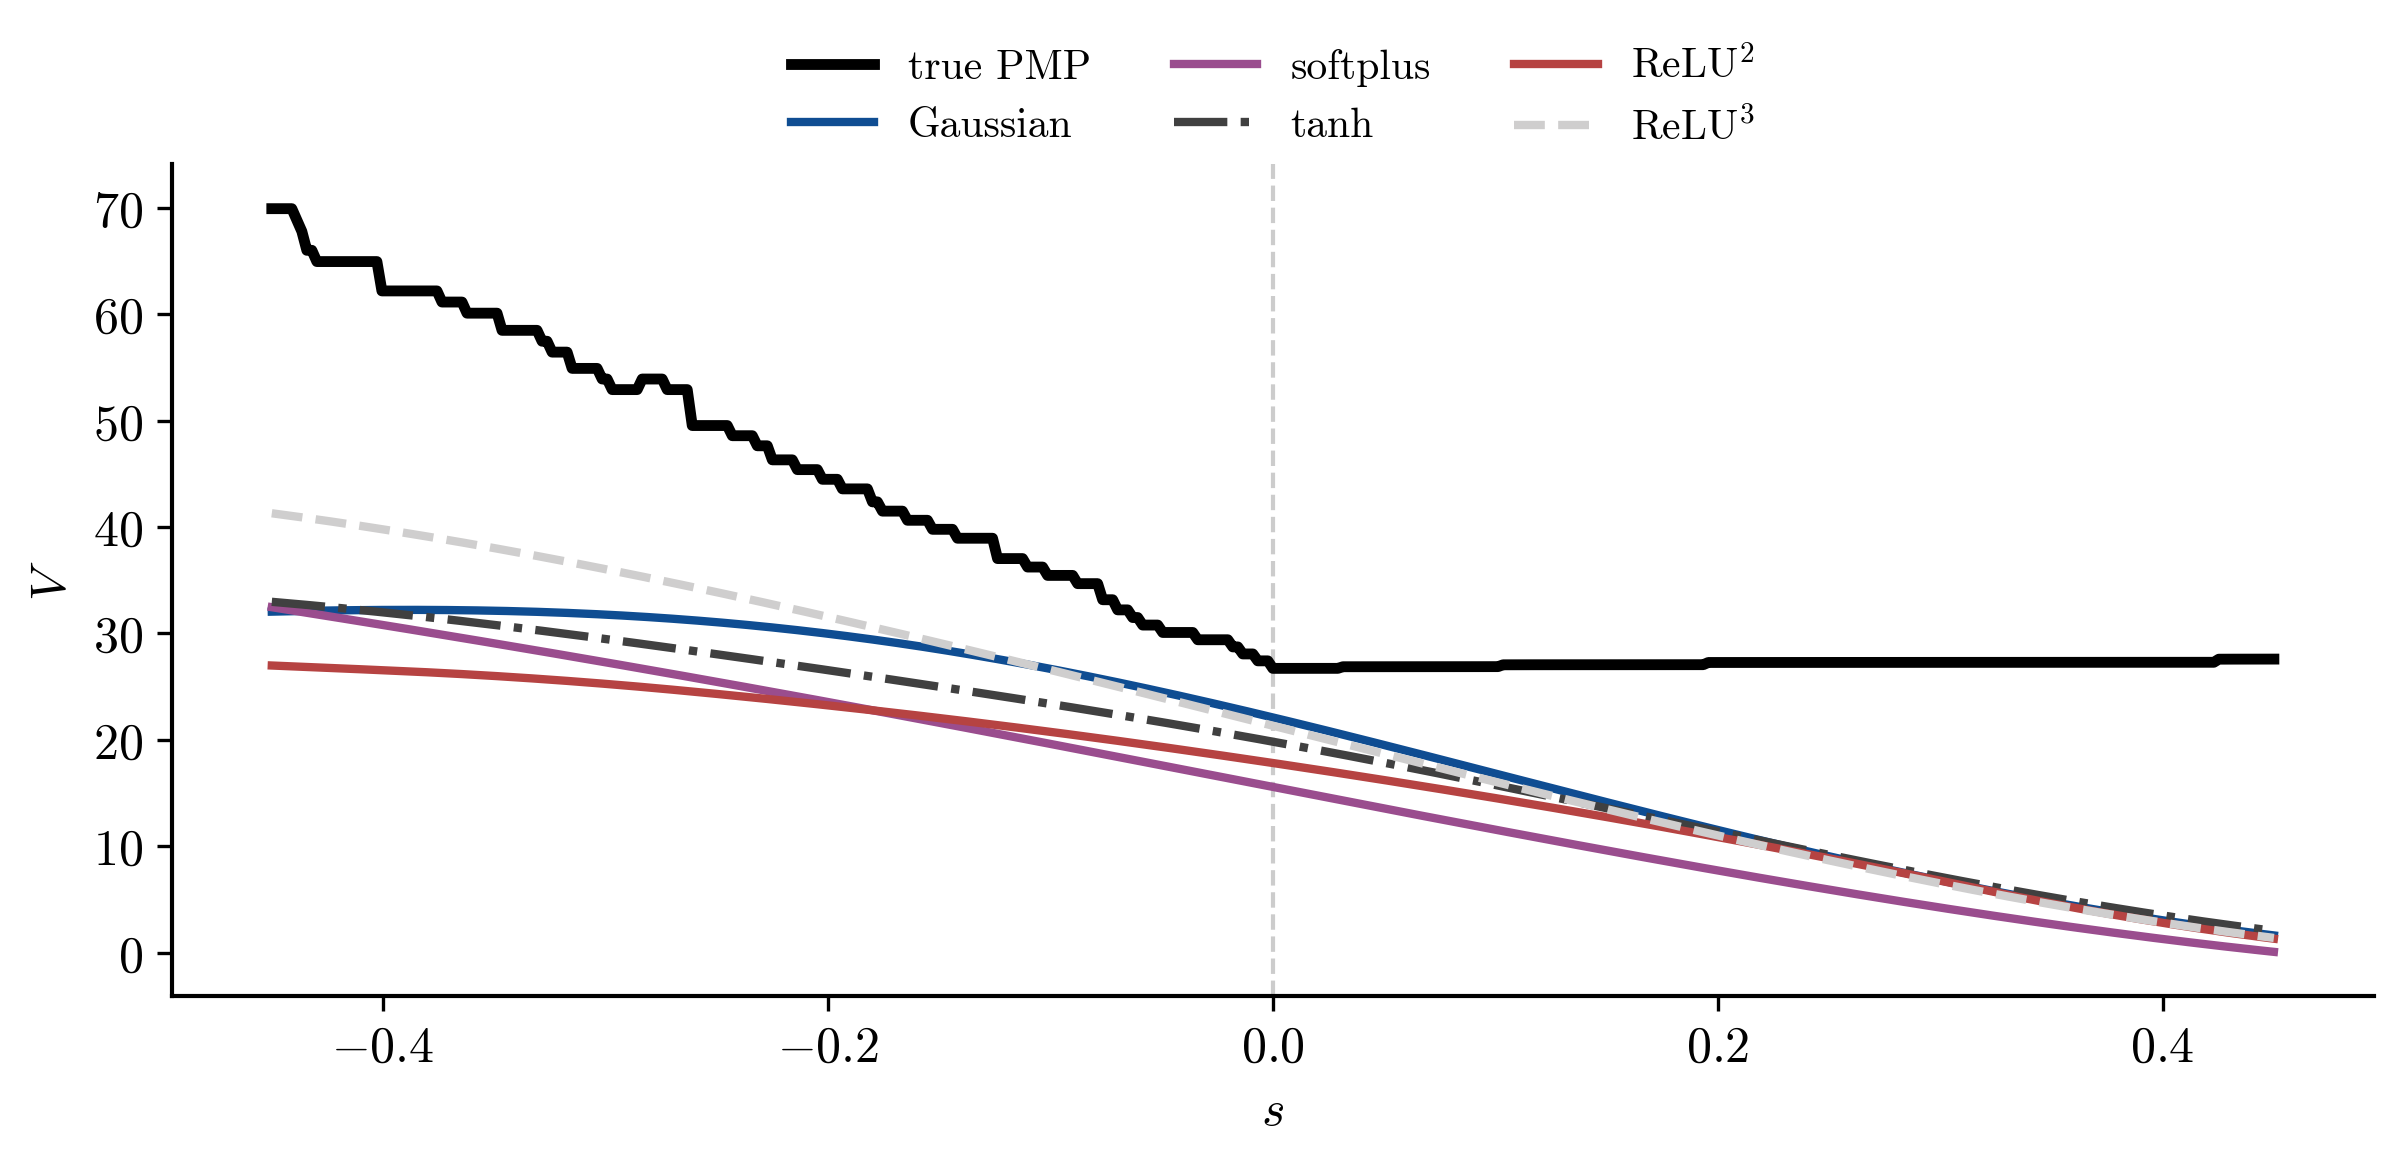
\includegraphics[width=\textwidth]{../experiments/02_pendulum/paper_log_penalty/figures/transect_value.png}
\caption{value $V$ along the normal.}
\label{fig:rs_transect_value}
\end{subfigure}
\hfill
\begin{subfigure}[b]{0.48\textwidth}
\centering
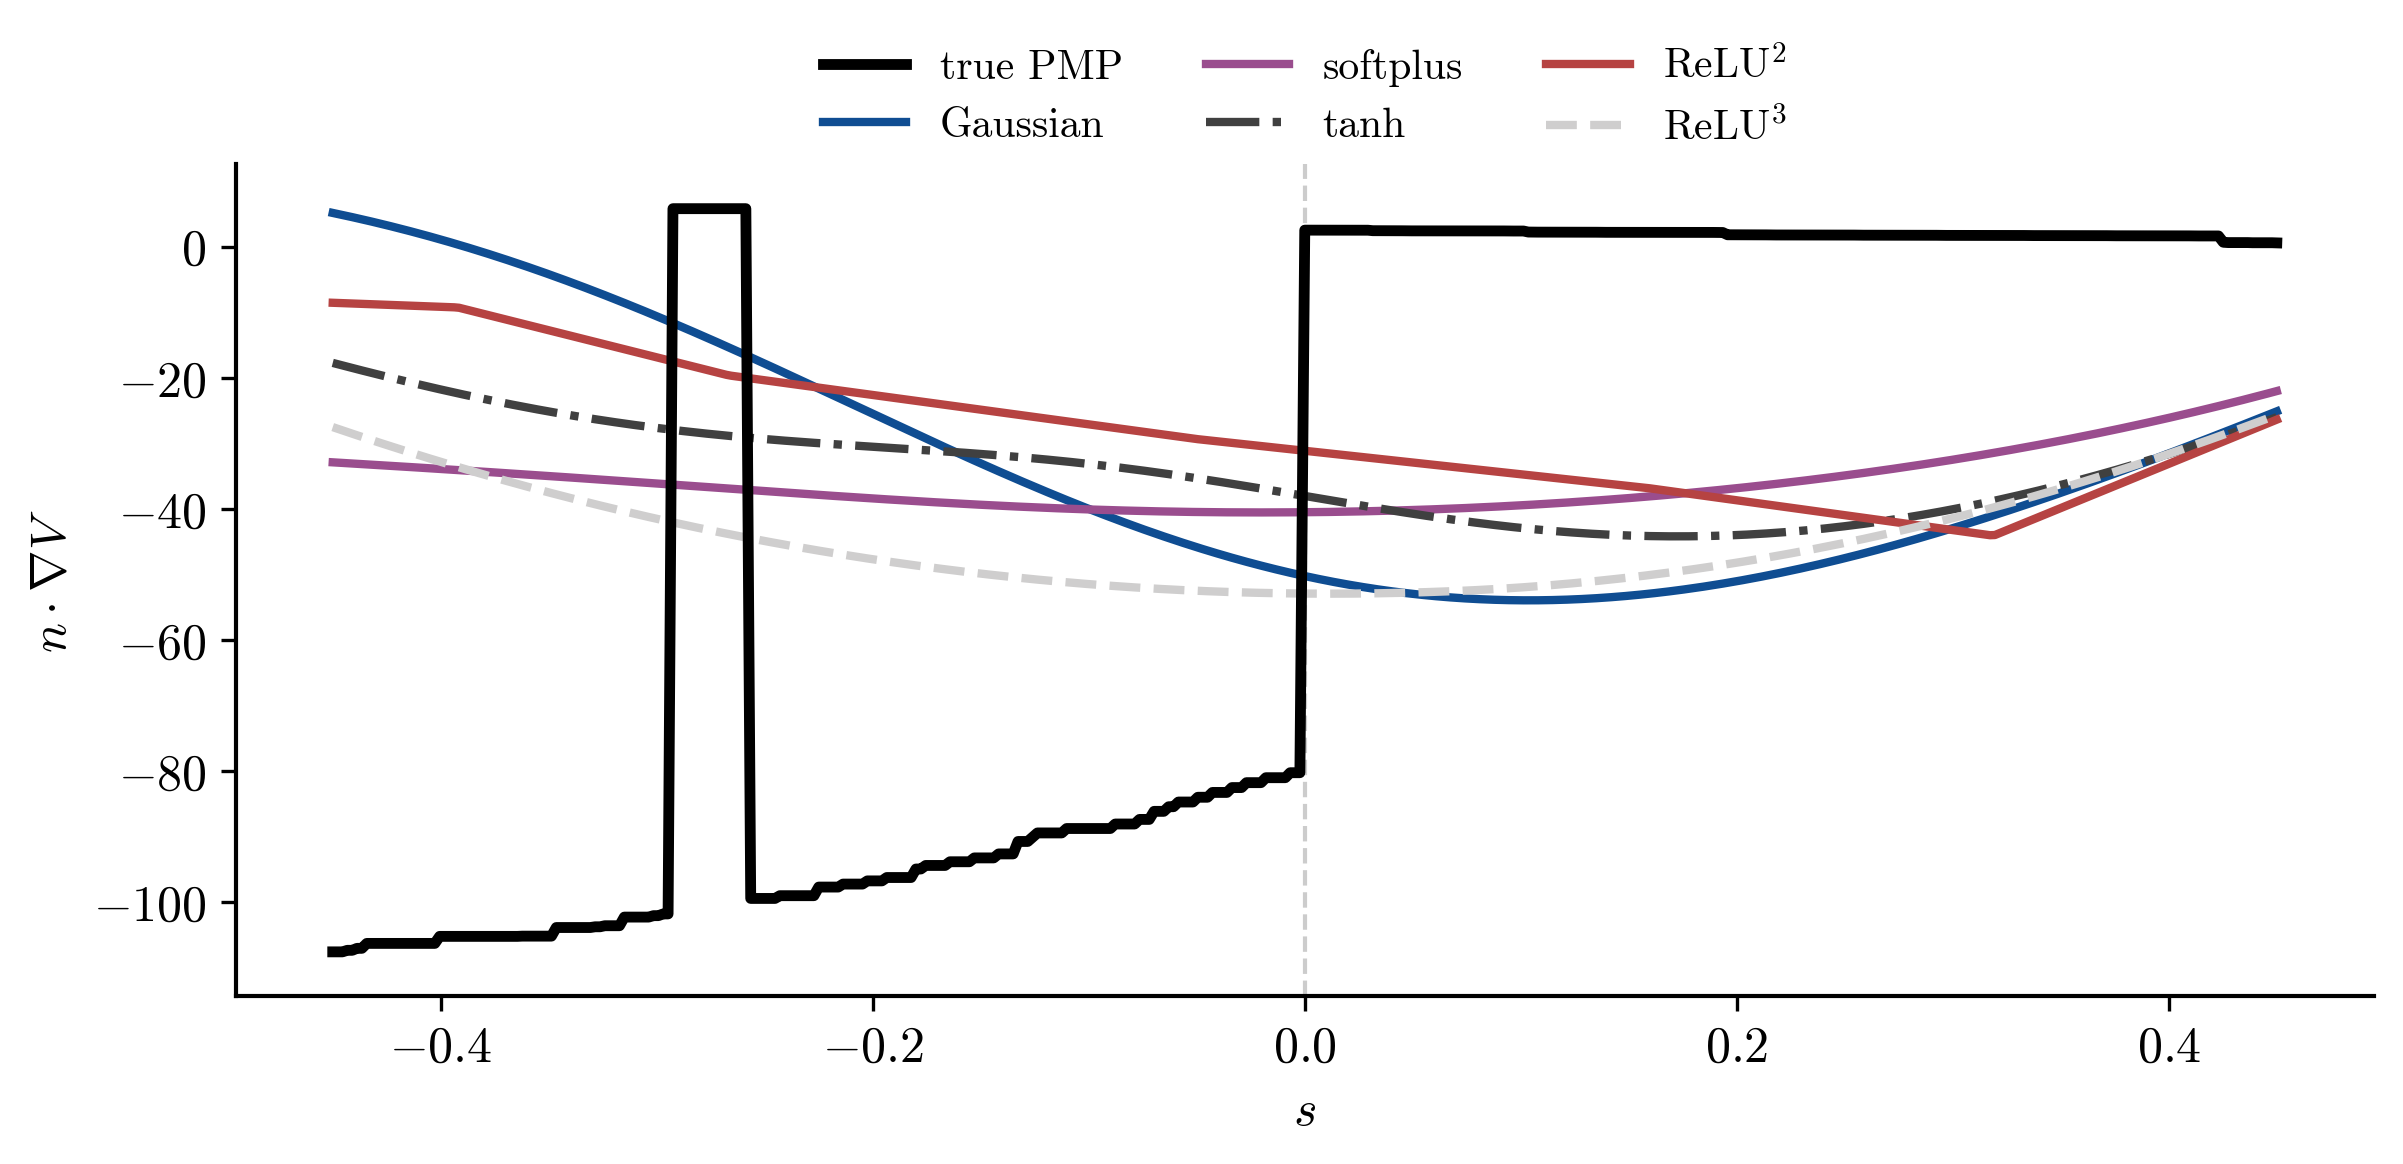
\includegraphics[width=\textwidth]{../experiments/02_pendulum/paper_log_penalty/figures/transect_normal_gradient.png}
\caption{normal gradient $n\cdot\nabla V$ along the normal.}
\label{fig:rs_transect_gradient}
\end{subfigure}
\caption{Normal cross-section of the switching curve, parametrized by the normal
distance $s$. Left: the true value (dashed)
is $\min\{V_0,V_{2\pi}\}$ on this cross-section and has a kink at $s=0$.
Right: the true normal
gradient jumps at $s=0$; $\mathrm{ReLU}^{2}$ develops the sharpest fitted
change of slope, while the smooth models interpolate through the
discontinuity. The rectangular
excursion of the reference curve near $s\approx-0.3$ is a nearest-neighbor
artifact in the evaluation of $\min\{V_0,V_{2\pi}\}$, not a feature of $V$.}
\label{fig:rs_transect}
\end{figure}


We next ask whether adding samples near $S$ reduces the error on $S_{0.3}$.
We compare $6{,}000$-sample sets containing $23\%$, $40\%$, or $60\%$ of
their samples near $S$ with a set obtained by adding $2{,}000$ such samples
to the first set. The Gaussian and $\mathrm{ReLU}^2$ networks are evaluated
on the same disjoint set of approximately $9.4\times10^5$ points.

\begin{table}[htbp]
\centering
\setlength{\tabcolsep}{12pt}
\renewcommand{\arraystretch}{1.25}
\begin{tabular}{llcc}
\toprule
Model & Training set & $S_{0.3}$ & $D\setminus S_{0.3}$ \\
\midrule
Gaussian & 6k, $23\%$ near $S$ & $2.78 \times 10^{-1}$ & $1.36 \times 10^{-1}$ \\
 & 6k, $40\%$ near $S$ & $2.76 \times 10^{-1}$ & $1.58 \times 10^{-1}$ \\
 & 6k, $60\%$ near $S$ & $2.99 \times 10^{-1}$ & $1.79 \times 10^{-1}$ \\
 & 6k $+$ 2k near $S$ & $2.96 \times 10^{-1}$ & $1.65 \times 10^{-1}$ \\
\midrule
$\mathrm{ReLU}^{2}$ & 6k, $23\%$ near $S$ & $2.70 \times 10^{-1}$ & $1.62 \times 10^{-1}$ \\
 & 6k, $40\%$ near $S$ & $2.84 \times 10^{-1}$ & $1.50 \times 10^{-1}$ \\
 & 6k, $60\%$ near $S$ & $3.22 \times 10^{-1}$ & $2.66 \times 10^{-1}$ \\
 & 6k $+$ 2k near $S$ & $3.00 \times 10^{-1}$ & $1.78 \times 10^{-1}$ \\
\bottomrule
\end{tabular}
\caption{Relative $H^1$ error on $S_{0.3}$ and $D\setminus S_{0.3}$. For each
model and training set, the table reports the result with the smallest error on
$S_{0.3}$ among the three tested values of $\alpha$, with every entry in that
row taken from the same run. The Gaussian uses $(\gamma,p)=(0,2.01)$ and
$\alpha\in\{10^{-3},10^{-4},10^{-5}\}$; $\mathrm{ReLU}^2$ uses $\psi_2$ and
$\alpha\in\{10^{-4},10^{-5},10^{-6}\}$. Errors are computed after
un-normalizing, so the two blocks share one definition.}
\label{tab:rs_oversampling}
\end{table}

For the tested sets, increasing the proportion of samples near $S$ produces no
systematic or material reduction in the error on $S_{0.3}$
(Table~\ref{tab:rs_oversampling}). Thus the observed difficulty is not resolved
by additional local samples.

\subsubsection{Validation and regional errors}
\label{sec:switching-comparison}

Figure~\ref{fig:rs_frontier}
tracks the best relative $H^{1}$ validation error reached as neurons are
inserted, for each activation paired with its penalty. The three
nonhomogeneous activations use the parameter values in
Figure~\ref{fig:neuron_h1_frontier}\subref{fig:feedback_cost_a};
the rectified powers use $\psi_k$ with $\alpha=10^{-6}$ for both $k=2$ and
$k=3$. The $k=2$ fit reaches the smallest validation error, approximately
$3.13\times10^{-1}$, followed by the Gaussian at $3.61\times10^{-1}$,
$\mathrm{ReLU}^{3}$ at $4.03\times10^{-1}$, $\tanh$ at
$4.06\times10^{-1}$, and softplus at $5.31\times10^{-1}$.

\begin{figure}[htbp]
\centering
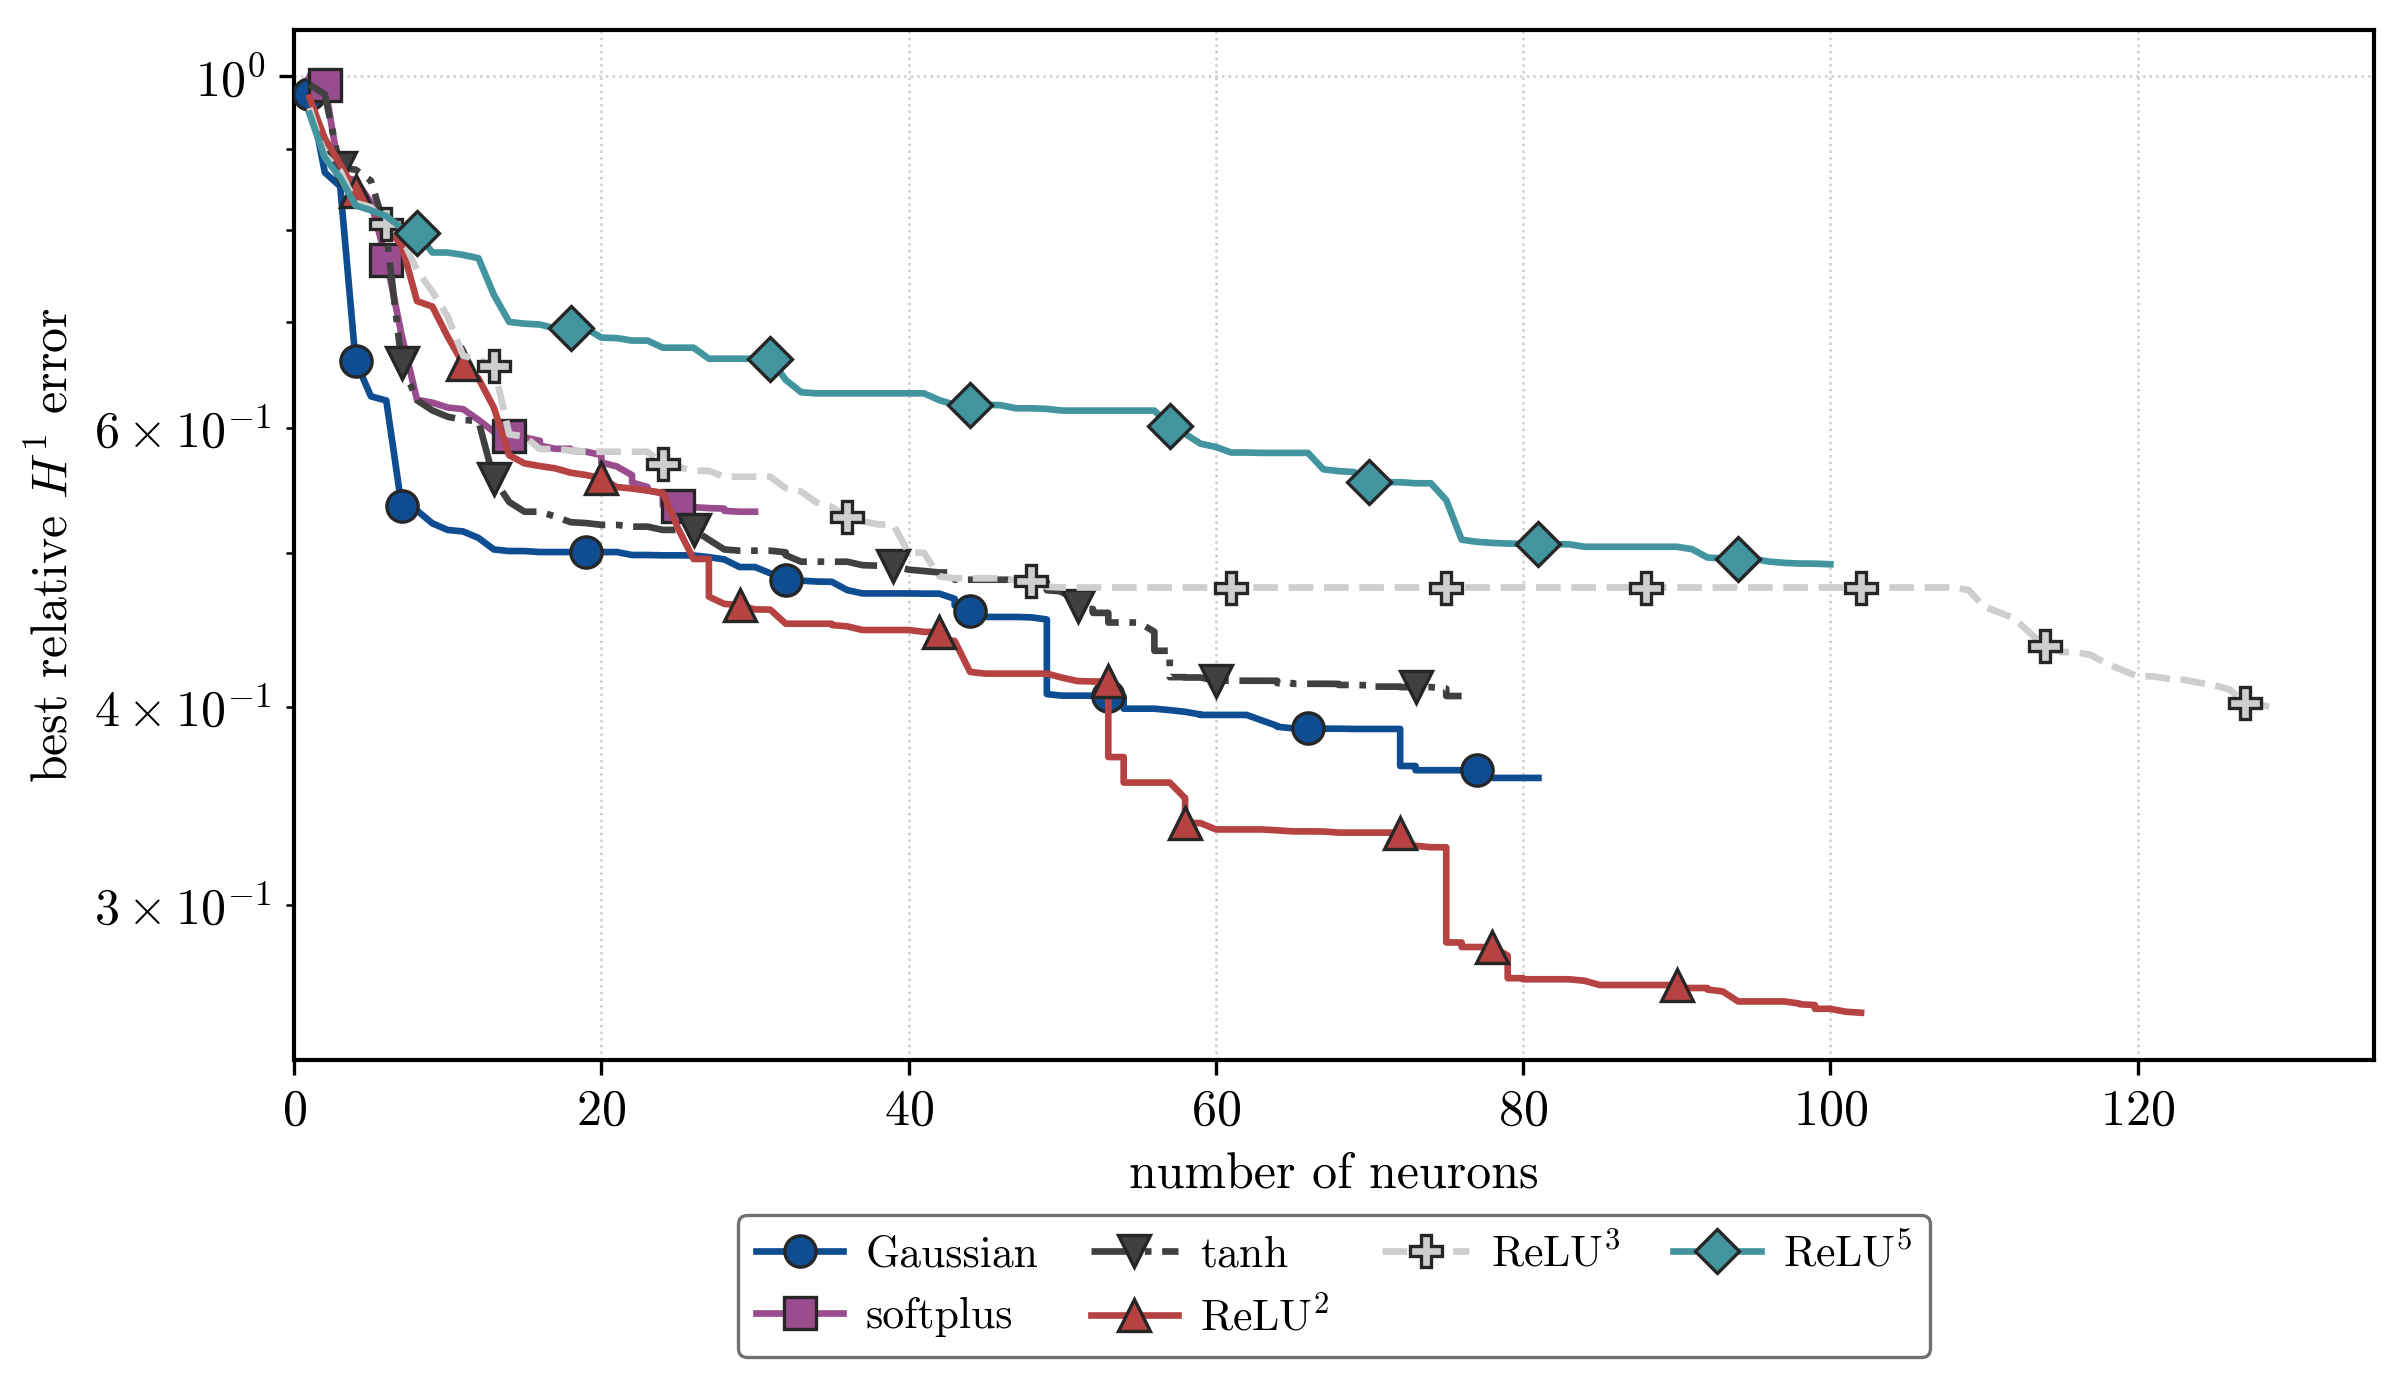
\includegraphics[width=0.7\textwidth]{../experiments/02_pendulum/paper_log_penalty/figures/frontier.png}
\caption{Best relative $H^{1}$ validation error against
neuron count. The nonhomogeneous activations use
\eqref{eq:empirical-log-objective}; the homogeneous activations use
$J^M_{\psi_k}$ with $\alpha=10^{-6}$ for both $k=2$ and $k=3$.}
\label{fig:rs_frontier}
\end{figure}

Figure~\ref{fig:rs_dumbbell} reports
the relative $H^{1}$ error on a separate evaluation set of approximately
$9.6\times10^{5}$ points. Training rows are excluded, and for each run we use
the recorded iterate with the smallest training objective. Errors are reported
on $S_{0.3}$ and $D\setminus S_{0.3}$. The $\mathrm{ReLU}^{2}$ fit has the
smallest errors in both regions ($0.293$ and $0.175$). The corresponding
values are $0.304$ and $0.191$ for the Gaussian, $0.332$ and $0.449$ for
$\mathrm{ReLU}^{3}$, $0.358$ and $0.197$ for $\tanh$, and $0.501$ and
$0.417$ for softplus.

\begin{figure}[htbp]
\centering
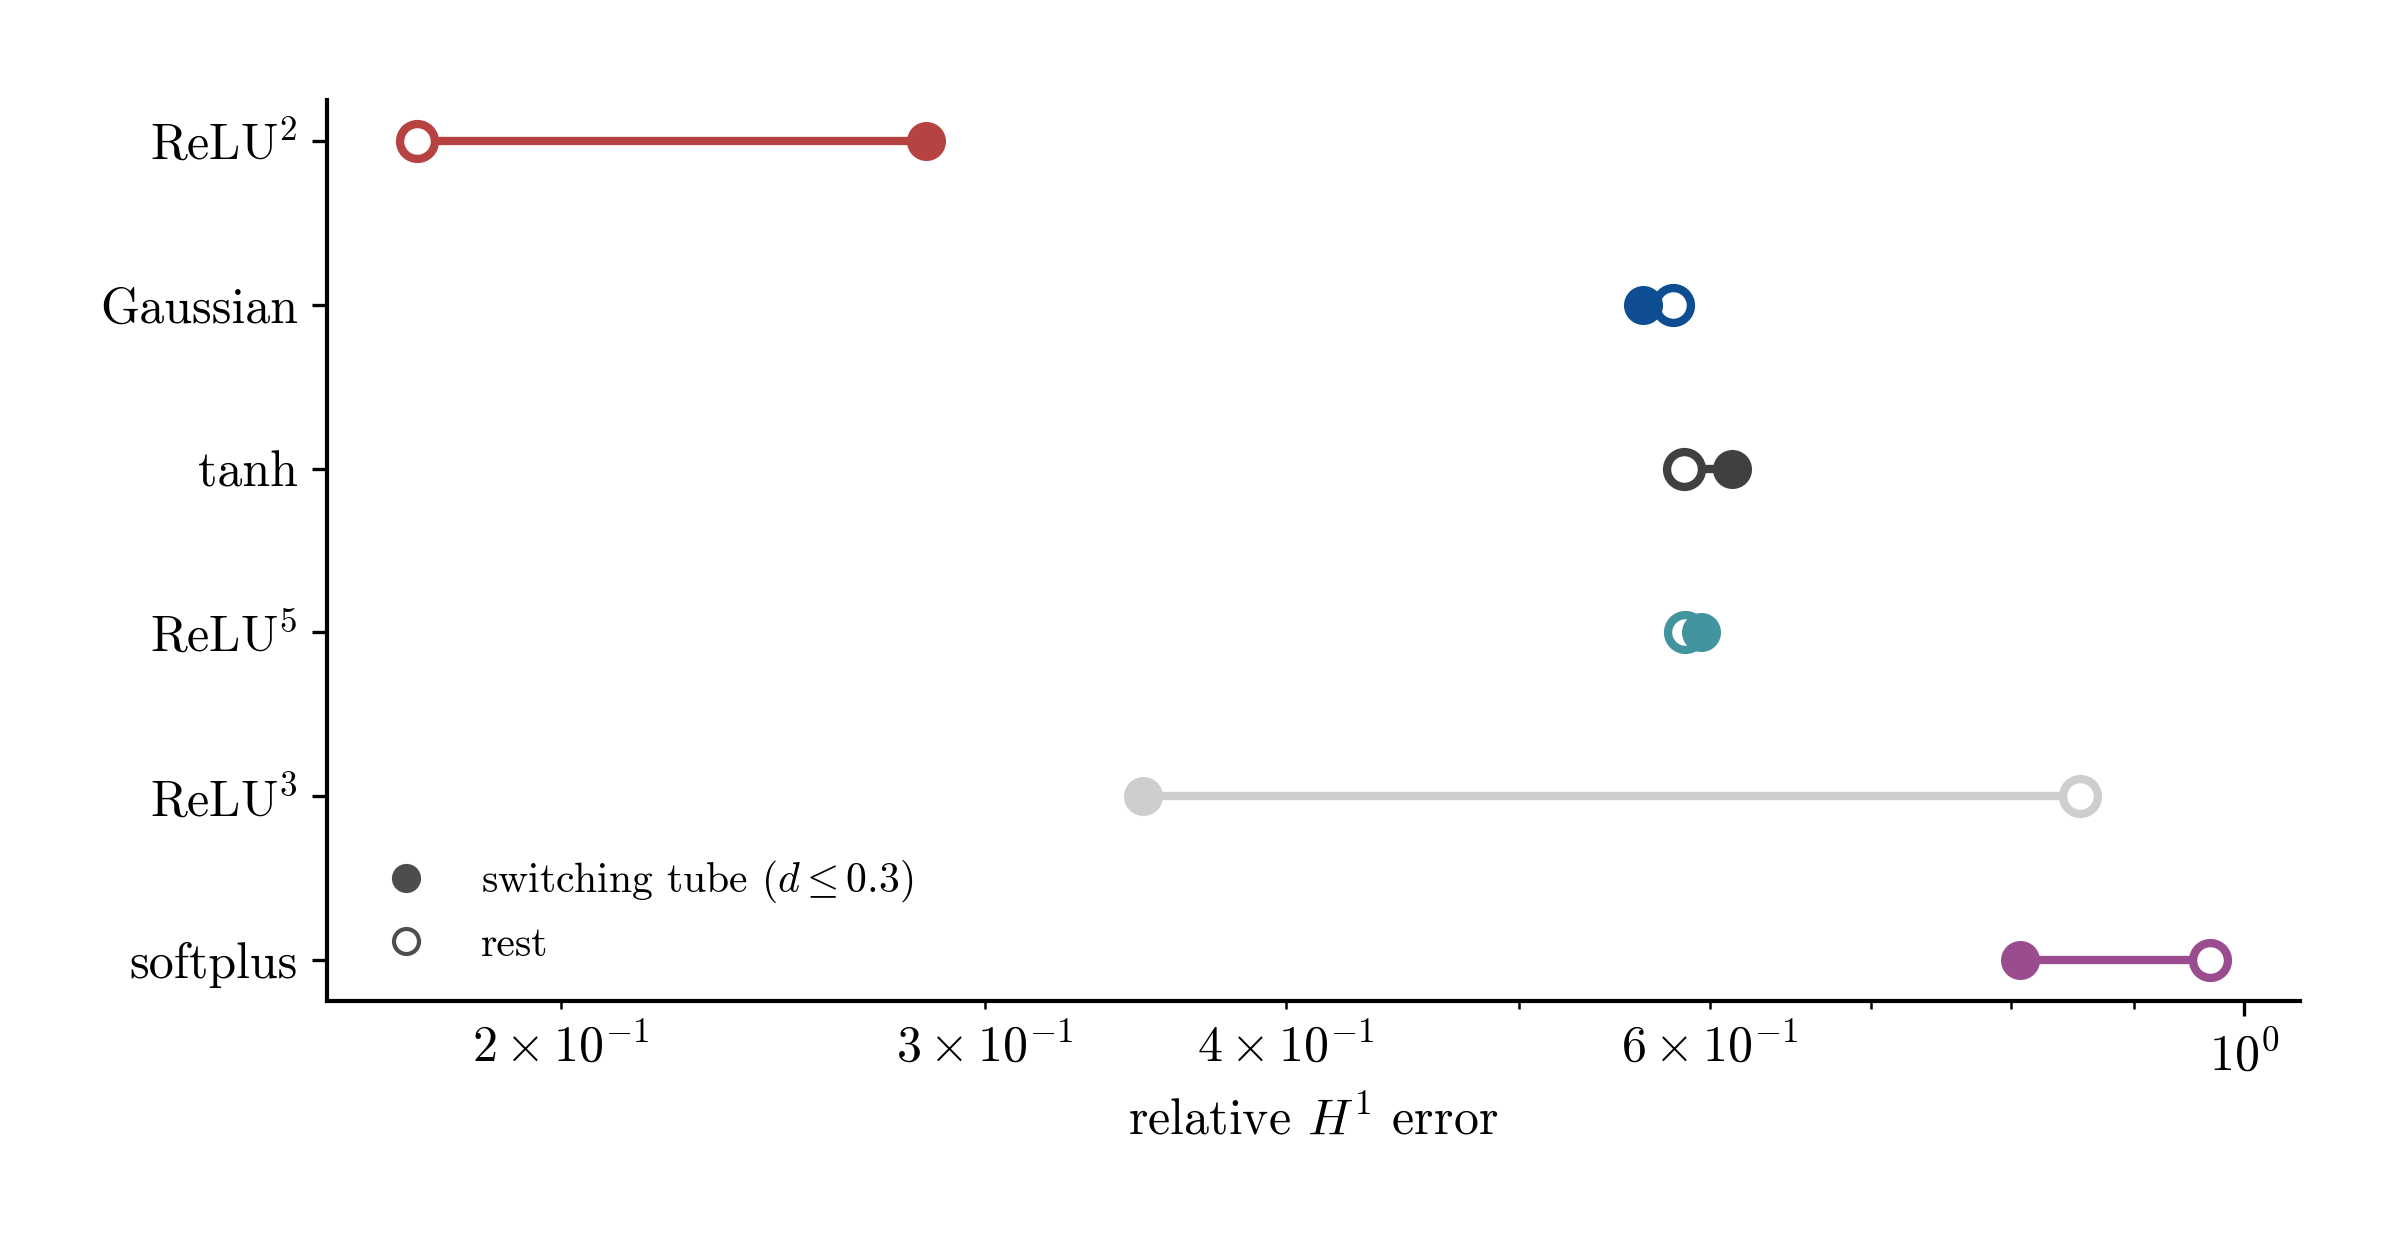
\includegraphics[width=0.8\textwidth]{../experiments/02_pendulum/paper_log_penalty/figures/near_far_dumbbell.png}
\caption{Relative $H^{1}$ error on $S_{0.3}$ (filled markers) and
$D\setminus S_{0.3}$ (open markers), with rows ordered by the latter error.}
\label{fig:rs_dumbbell}
\end{figure}



\subsubsection{Feedback synthesis across the switching set}
Minimizing the Hamiltonian in $u$ gives the optimal control in feedback form,
\begin{equation*}
u(x) = -\frac{1}{2\,\eta\,m\ell^{2}}\,\partial_{\dot{\theta}}V(x);
\end{equation*}
replacing $V$ by a fitted $\widehat V$ yields a candidate feedback law. We test
each law in closed loop from two initial states placed on either side of the
switching curve, $A=(0.71,\,0.68)$ and $B=(0.23,\,0.53)$, integrating the
dynamics over the horizon $T=10$ with fixed-step RK4 ($\Delta t = 5\times10^{-3}$),
zero-order-hold controls, and the numerical bound $|u|\le30$ (the OCP itself
is unconstrained). The optimal paths from the two starts are different. From
$A$, the optimal law swings the pendulum over the top to the
upright at $\theta=2\pi$, while from $B$ it brakes directly to the upright at
$\theta=0$. Thus it must select the path associated with $V_{2\pi}$ at
$A$ and the path associated with $V_0$ at $B$. The reference law uses
the $40$ nearest raw PMP samples to compare $V_0$ and $V_{2\pi}$ and applies
the feedback formula using the costate associated with the smaller value.

\begin{figure}[htbp]
\centering
\captionsetup[subfigure]{justification=centering}
\begin{subfigure}[b]{0.32\textwidth}
\centering
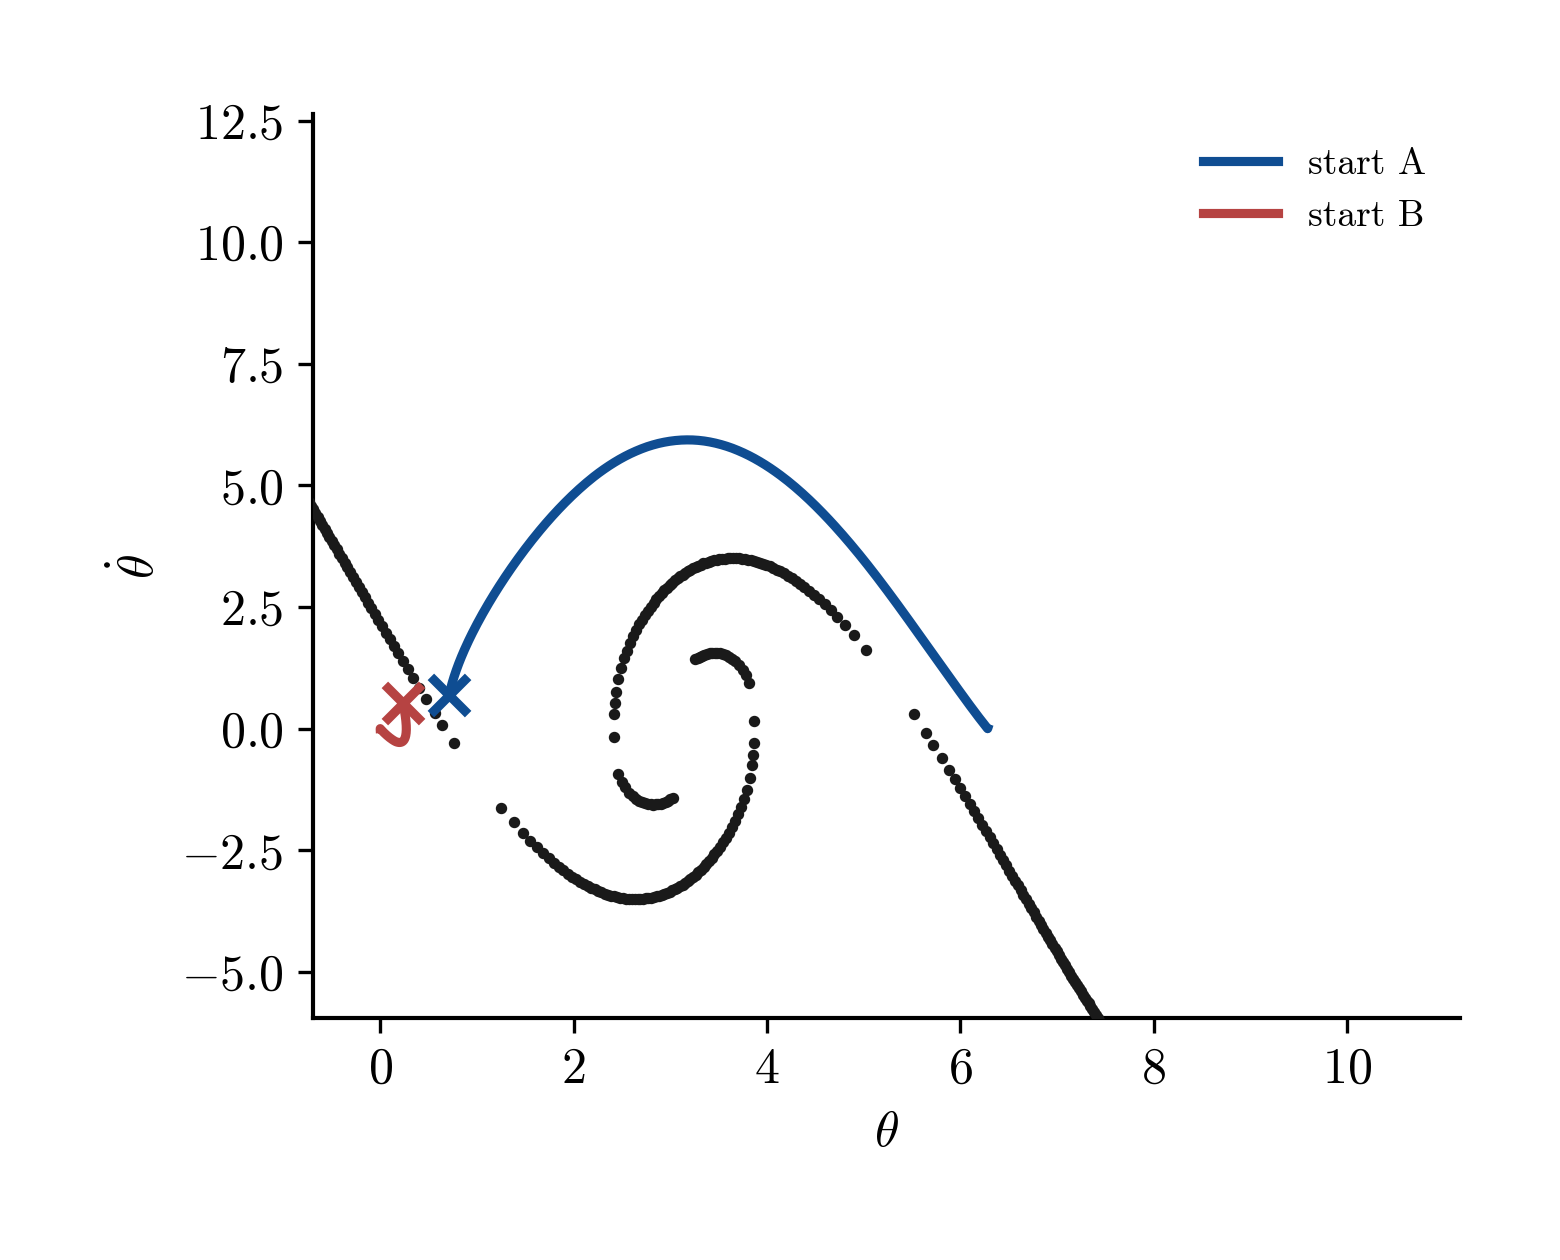
\includegraphics[width=\textwidth]{../experiments/02_pendulum/paper_log_penalty/figures/feedback_true_pmp.png}
\caption{reference (PMP)}
\label{fig:rs_feedback_true}
\end{subfigure}
\hfill
\begin{subfigure}[b]{0.32\textwidth}
\centering
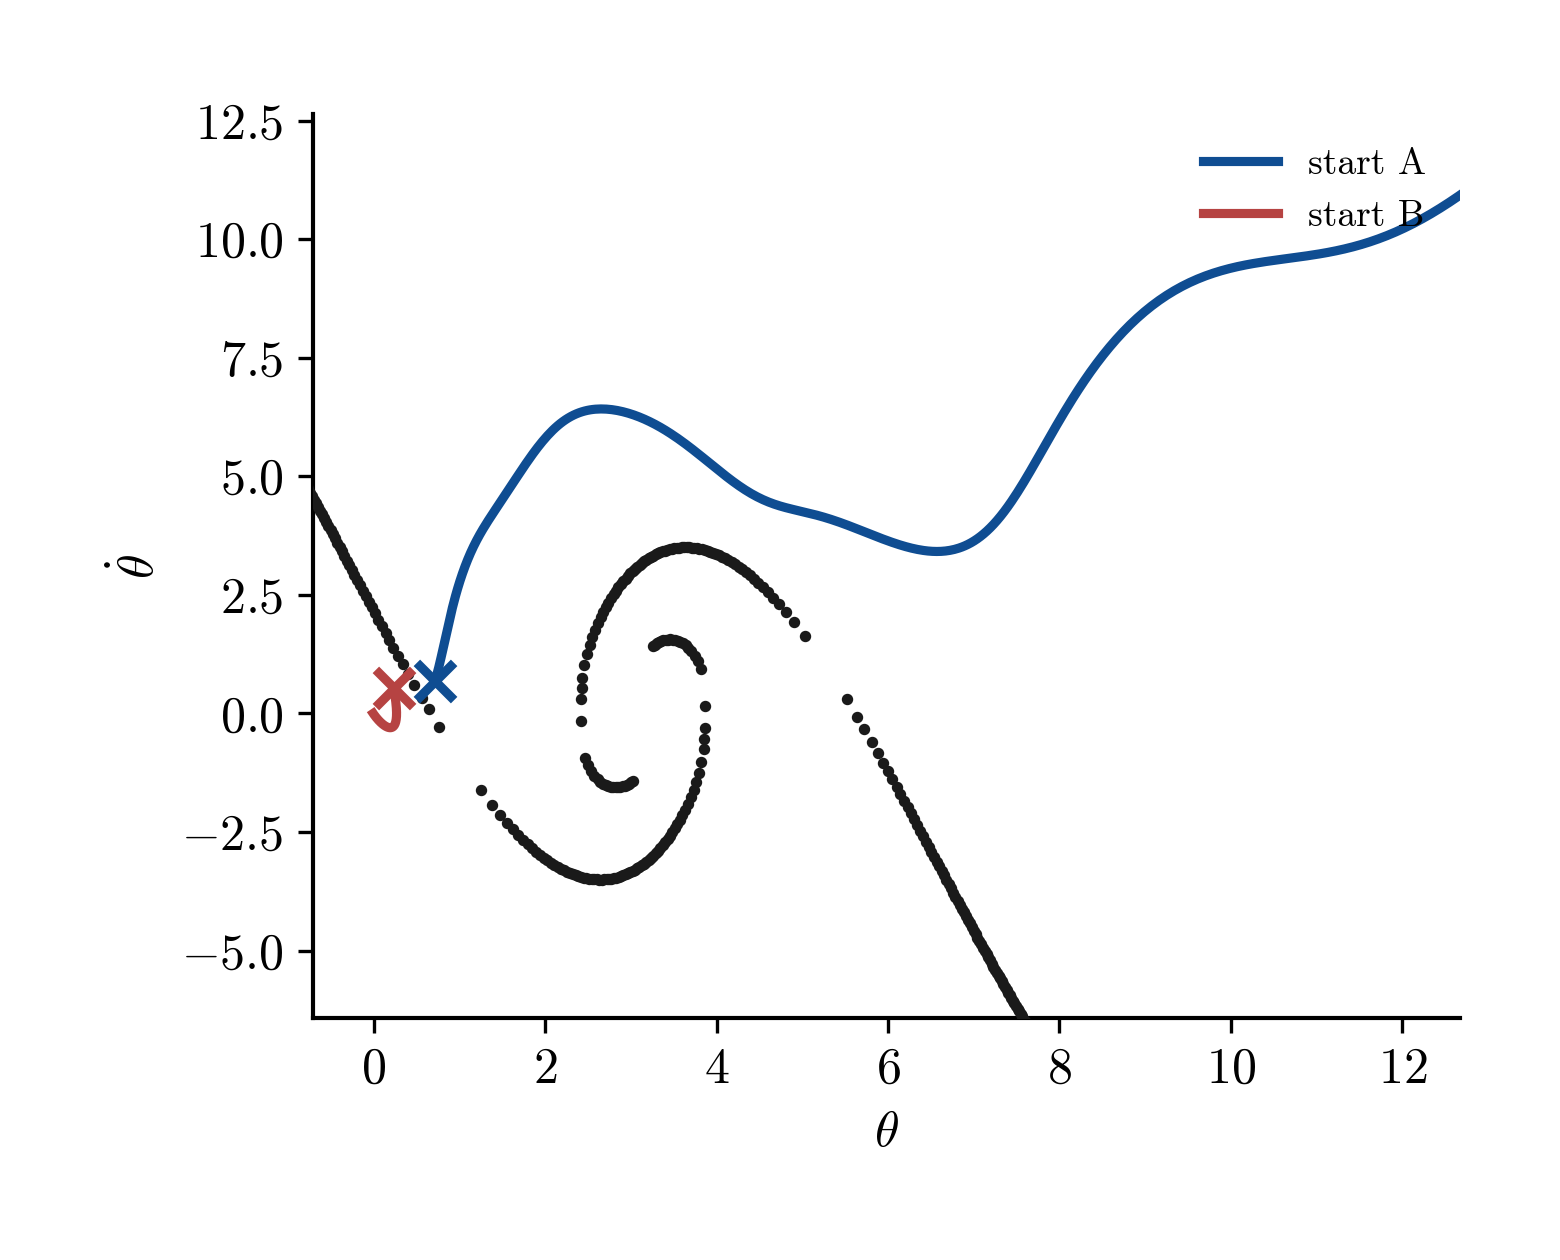
\includegraphics[width=\textwidth]{../experiments/02_pendulum/paper_log_penalty/figures/feedback_gaussian.png}
\caption{Gaussian}
\label{fig:rs_feedback_gaussian}
\end{subfigure}
\hfill
\begin{subfigure}[b]{0.32\textwidth}
\centering
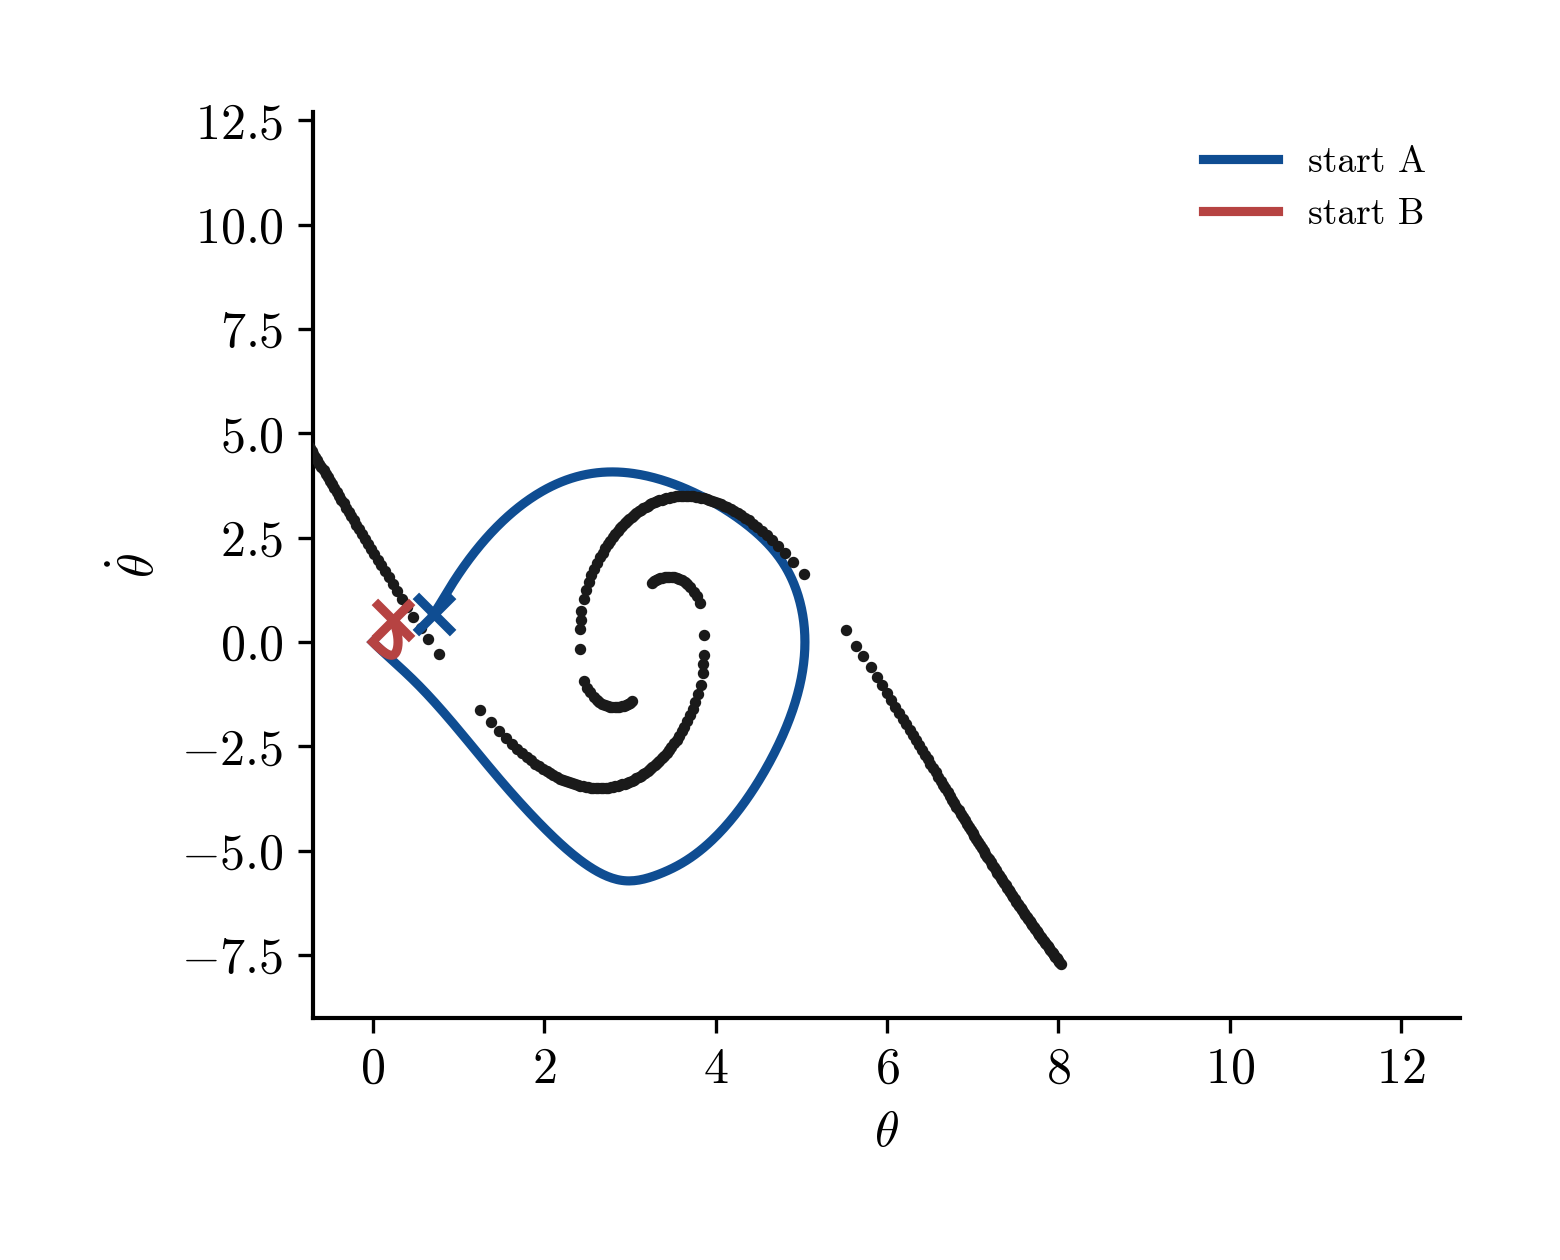
\includegraphics[width=\textwidth]{../experiments/02_pendulum/paper_log_penalty/figures/feedback_softplus.png}
\caption{softplus}
\label{fig:rs_feedback_softplus}
\end{subfigure}
\vspace{0.6em}
\begin{subfigure}[b]{0.32\textwidth}
\centering
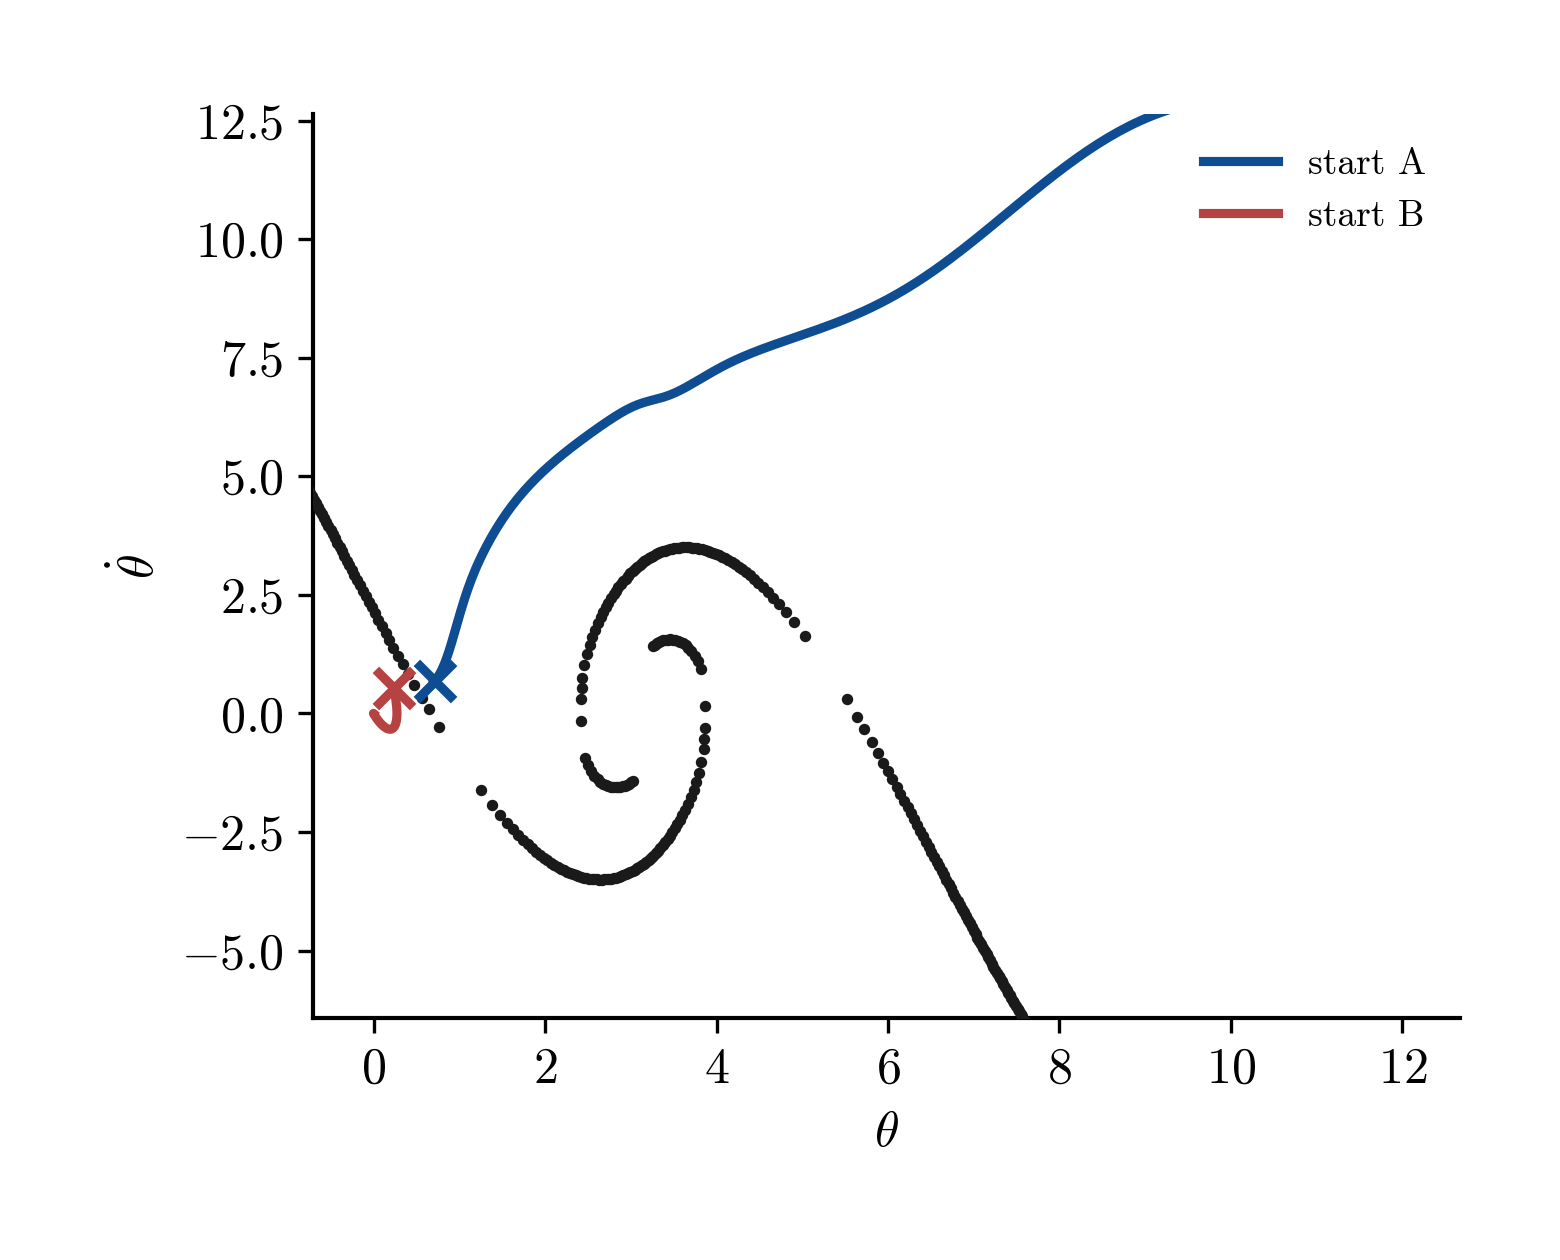
\includegraphics[width=\textwidth]{../experiments/02_pendulum/paper_log_penalty/figures/feedback_tanh.png}
\caption{$\tanh$}
\label{fig:rs_feedback_tanh}
\end{subfigure}
\hfill
\begin{subfigure}[b]{0.32\textwidth}
\centering
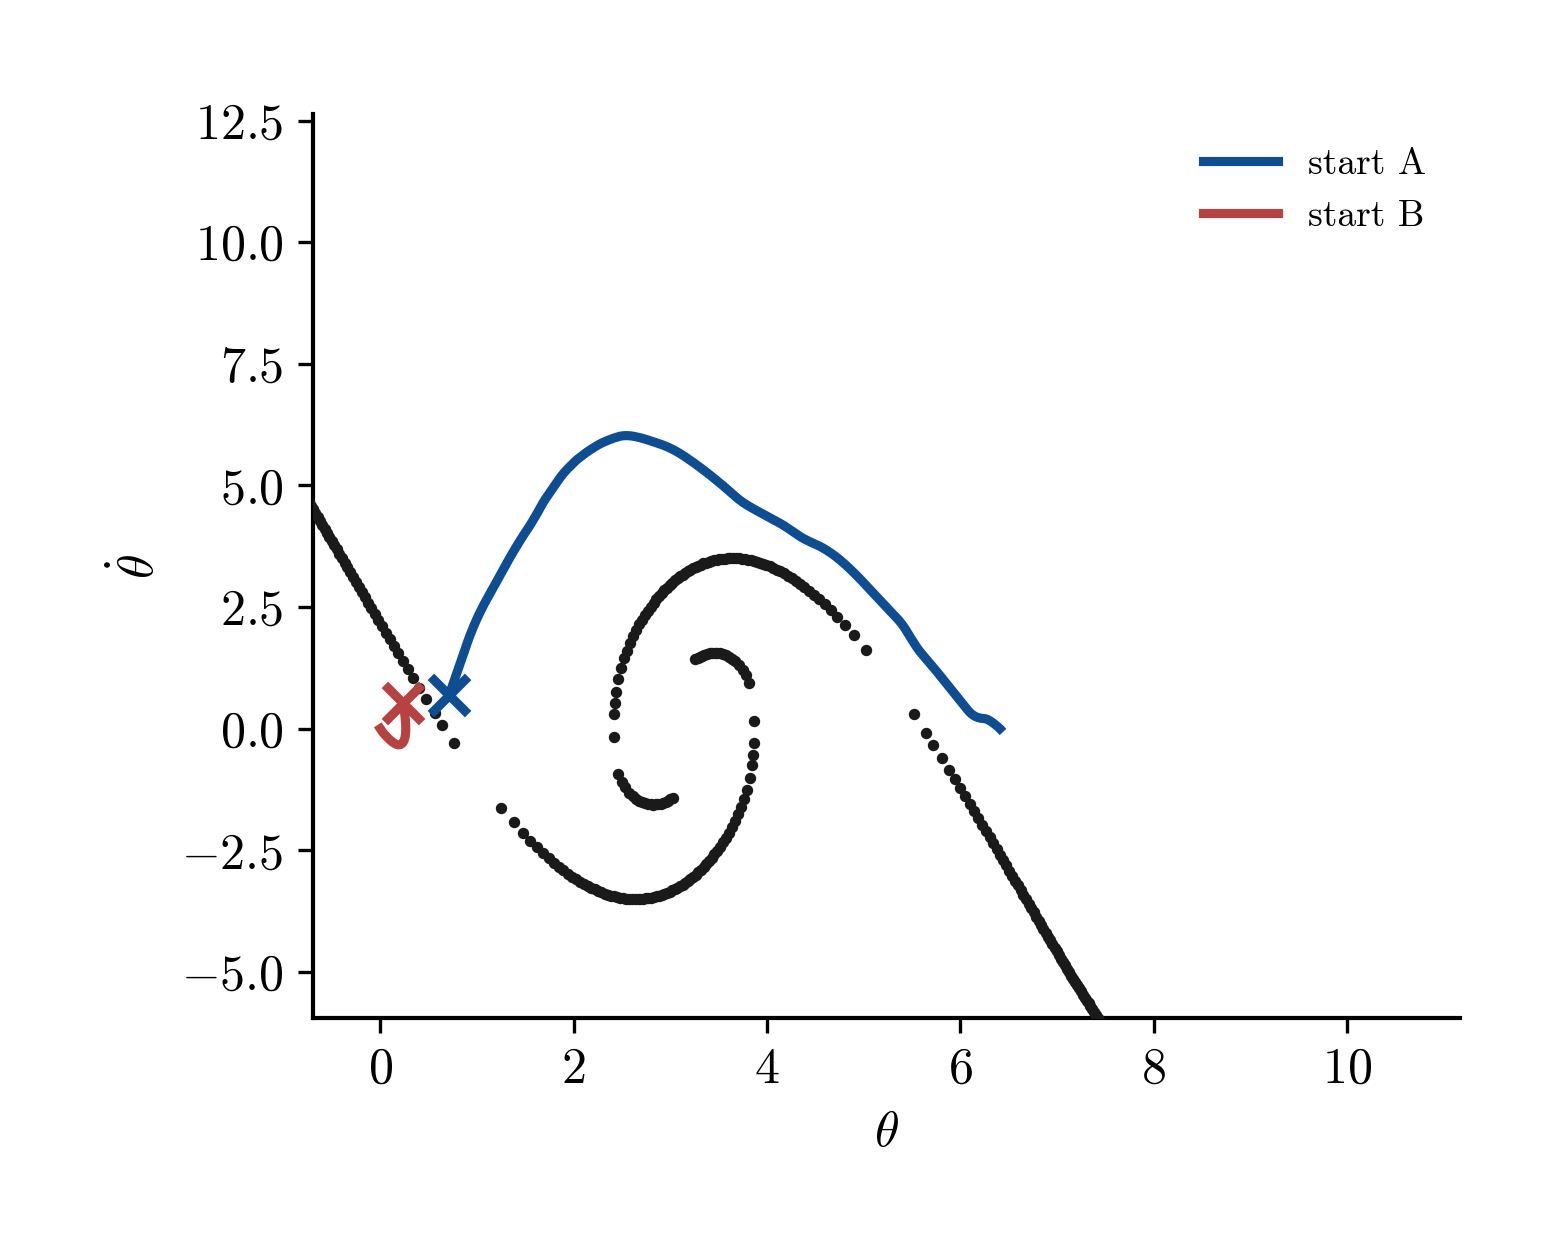
\includegraphics[width=\textwidth]{../experiments/02_pendulum/paper_log_penalty/figures/feedback_relu2.png}
\caption{$\mathrm{ReLU}^{2}$ + $\psi_{2}$}
\label{fig:rs_feedback_relu2}
\end{subfigure}
\hfill
\begin{subfigure}[b]{0.32\textwidth}
\centering
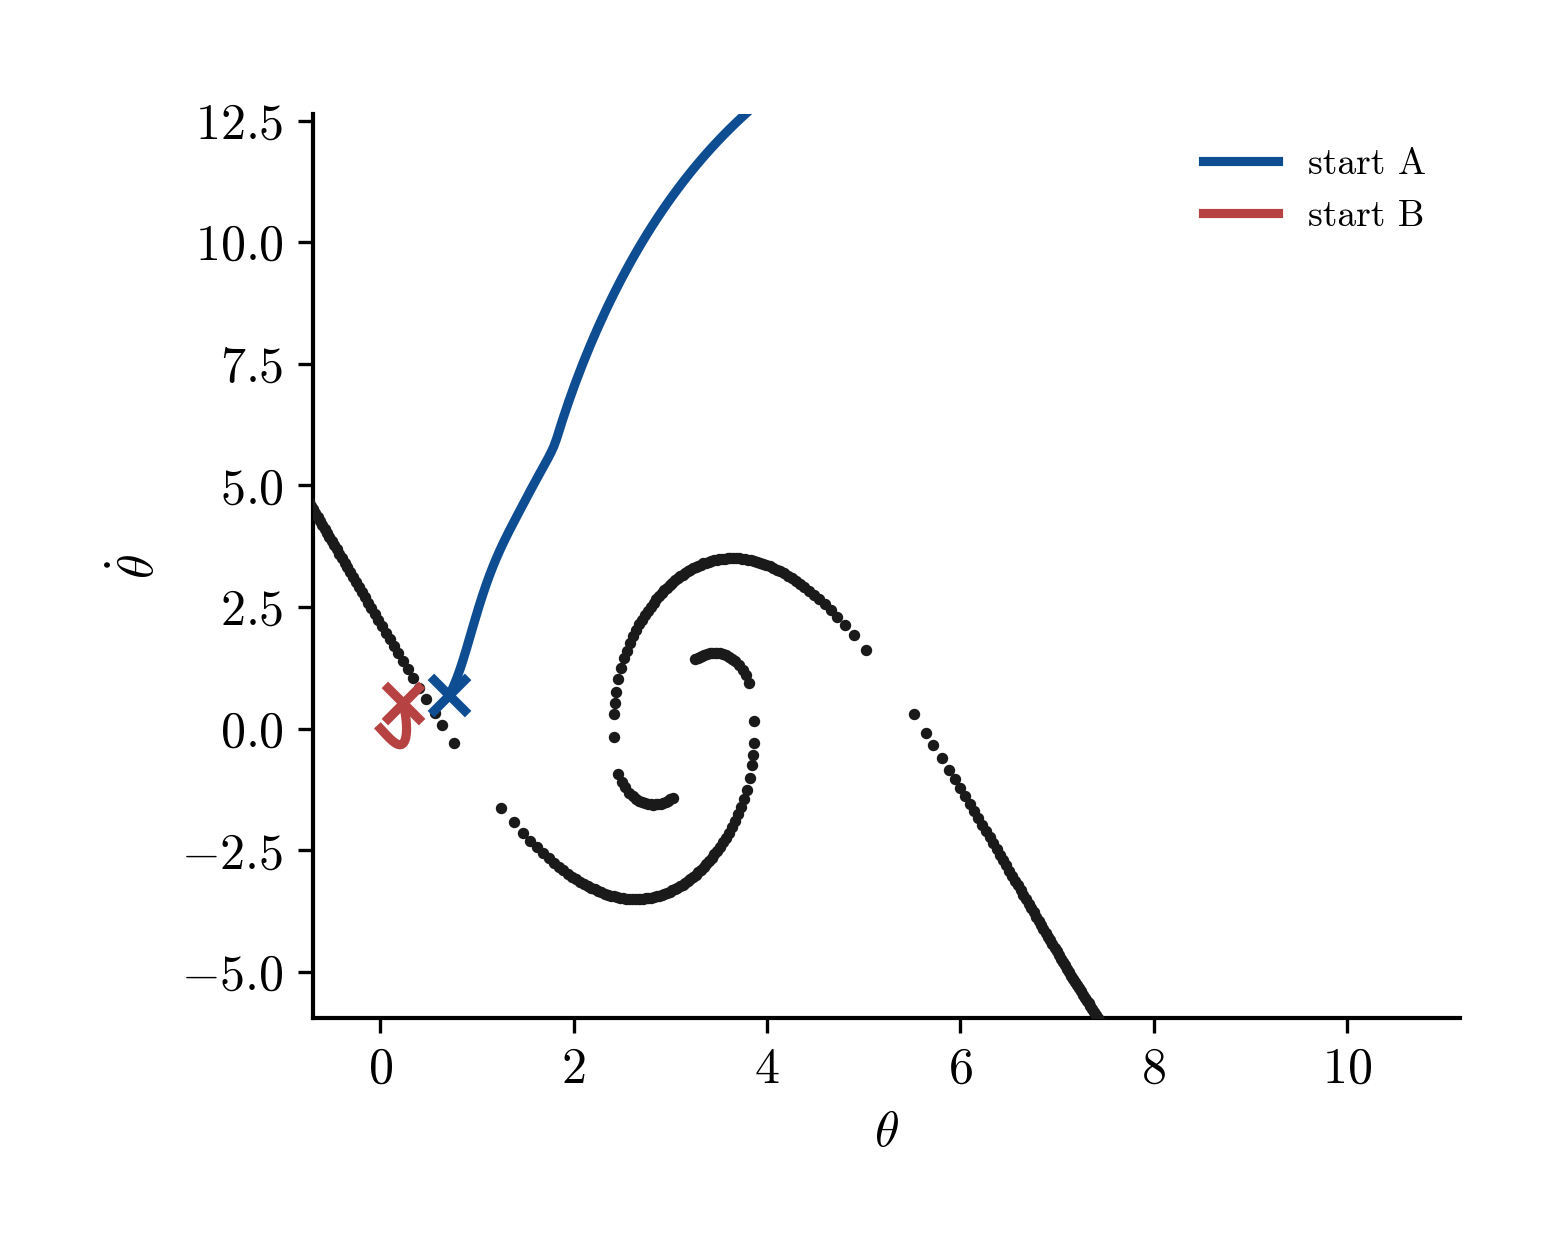
\includegraphics[width=\textwidth]{../experiments/02_pendulum/paper_log_penalty/figures/feedback_relu3.png}
\caption{$\mathrm{ReLU}^{3}$ + $\psi_{3}$}
\label{fig:rs_feedback_relu3}
\end{subfigure}
\caption{Closed-loop paths in the $(\theta,\dot\theta)$ plane from the
two starts $A$ (blue) and $B$ (red) on either side of the switching curve
(black), one panel per feedback law; all panels share the same axes. The
reference law swings over the top from $A$ and brakes to $\theta=0$ from $B$.
Softplus, $\mathrm{ReLU}^{2}$, and $\mathrm{ReLU}^{3}$ reach an upright
neighbourhood from both starts; the Gaussian and $\tanh$ reach one only from
$B$.}
\label{fig:rs_feedback}
\end{figure}

From the harder start $A$, softplus, $\mathrm{ReLU}^{2}$, and
$\mathrm{ReLU}^{3}$ reach the upright neighbourhood, at costs $69.8$, $60.4$,
and $103.2$, respectively
(Figure~\ref{fig:neuron_h1_frontier}\subref{fig:feedback_cost_a}). The
Gaussian, $\tanh$, and ReLU--$\ell^1$ laws do not satisfy the terminal
criterion from this start.
Figure~\ref{fig:rs_feedback_control} shows the control signal from $A$.
The reference starts with a control close to zero, whereas every fitted law
starts with a substantially larger negative control and consequently follows
a different closed-loop trajectory.

\begin{figure}[htbp]
\centering
\captionsetup[subfigure]{justification=centering}
\begin{subfigure}[b]{0.48\textwidth}
\centering
\includegraphics[width=\textwidth]{../experiments/02_pendulum/paper_log_penalty/figures/feedback_control_a_log_penalty.png}
\caption{Algorithm~\ref{alg:log}.}
\label{fig:rs_feedback_control_log}
\end{subfigure}
\hfill
\begin{subfigure}[b]{0.48\textwidth}
\centering
\includegraphics[width=\textwidth]{../experiments/02_pendulum/paper_log_penalty/figures/feedback_control_a_relu.png}
\caption{$\mathrm{ReLU}^{k}$ models.}
\label{fig:rs_feedback_control_relu}
\end{subfigure}
\caption{Feedback control $u(t)$ from start $A$, per law, beside the reference
(black). The reference initially applies almost no control and selects the
$2\pi$ swing-up branch. Every fitted law instead starts with a much larger
negative control. After the trajectories separate, values at the same time
are evaluated at different states and are therefore not pointwise feedback
errors at a common state.}
\label{fig:rs_feedback_control}
\end{figure}

In summary, $\mathrm{ReLU}^{2}$ gives the smallest validation and regional
errors and reaches the upright from both starts. Softplus and
$\mathrm{ReLU}^{3}$ also reach it from both; their costs from $A$ are $69.8$
and $103.2$, respectively, compared with $60.4$ for $\mathrm{ReLU}^{2}$ and
$26.2$ for the reference. The Gaussian and $\tanh$ succeed only from $B$.

The regional approximation error and the binary terminal outcome contain
different information. The Gaussian and $\tanh$ fits are more accurate than
softplus on both reported regions, yet softplus makes the correct branch
decision from $A$ while they do not. Thus the switching-set error diagnoses
the difficulty of approximating the discontinuous gradient, but a reliable
feedback assessment still requires a closed-loop test.


\FloatBarrier

\section{Conclusion and outlook}

We developed a measure-theoretic framework for sparse, gradient-augmented
recovery of HJB value functions from PMP data. Its main contribution is a
variational route from infinitely wide dictionaries to finite shallow
networks for two activation classes that require different compactness
arguments. For nonhomogeneous activations, simultaneous normalization of the
measure and dictionary controls escape on the unbounded parameter domain and,
together with the concave penalty, yields existence, finite support,
separation and width bounds, and a quantitative decay rate for the excess
above the insertion threshold. For positively $k$-homogeneous activations,
radial optimization instead reduces the problem to the unit sphere and
induces a fractional-power penalty; the resulting formulation likewise admits
global minimizers and explicit finite-width conclusions. These results give a
rigorous foundation for constructing sparse networks that approximate both a
value function and its gradient.

The numerical studies illustrate the role and the boundary of this framework.
On the smooth Van der Pol problem, the proposed formulations produce sparse
approximants whose gradients define stabilizing feedback laws. On the
pendulum problem, they remain effective in the presence of a switching set,
but the experiments also show that regional $H^1$ error alone does not
determine the closed-loop branch decision. Thus gradient-augmented fitting is
a useful bridge from PMP data to feedback synthesis, while feedback
performance must still be assessed directly when the value gradient is
discontinuous.

The most immediate extension concerns the insertion step: the rate analysis
assumes exact global candidate maximization, whereas the implementation uses a
multistart local search. Developing certified or more reliable candidate
searches would therefore bring the algorithm closer to the theoretical
guarantee. A second direction is to complement the present approximation
criteria with feedback-aware training or validation near switching sets, and
then to examine the resulting methods in higher-dimensional control problems.

\newpage
\bibliographystyle{plain}
\bibliography{ref}
\end{document}
